\documentclass[twoside]{book}

% Packages required by doxygen
\usepackage{fixltx2e}
\usepackage{calc}
\usepackage{doxygen}
\usepackage[export]{adjustbox} % also loads graphicx
\usepackage{graphicx}
\usepackage[utf8]{inputenc}
\usepackage{makeidx}
\usepackage{multicol}
\usepackage{multirow}
\PassOptionsToPackage{warn}{textcomp}
\usepackage{textcomp}
\usepackage[nointegrals]{wasysym}
\usepackage[table]{xcolor}

% NLS support packages
\usepackage[spanish]{babel}
% Font selection
\usepackage[T1]{fontenc}
\usepackage[scaled=.90]{helvet}
\usepackage{courier}
\usepackage{amssymb}
\usepackage{sectsty}
\renewcommand{\familydefault}{\sfdefault}
\allsectionsfont{%
  \fontseries{bc}\selectfont%
  \color{darkgray}%
}
\renewcommand{\DoxyLabelFont}{%
  \fontseries{bc}\selectfont%
  \color{darkgray}%
}
\newcommand{\+}{\discretionary{\mbox{\scriptsize$\hookleftarrow$}}{}{}}

% Page & text layout
\usepackage{geometry}
\geometry{%
  a4paper,%
  top=2.5cm,%
  bottom=2.5cm,%
  left=2.5cm,%
  right=2.5cm%
}
\tolerance=750
\hfuzz=15pt
\hbadness=750
\setlength{\emergencystretch}{15pt}
\setlength{\parindent}{0cm}
\setlength{\parskip}{3ex plus 2ex minus 2ex}
\makeatletter
\renewcommand{\paragraph}{%
  \@startsection{paragraph}{4}{0ex}{-1.0ex}{1.0ex}{%
    \normalfont\normalsize\bfseries\SS@parafont%
  }%
}
\renewcommand{\subparagraph}{%
  \@startsection{subparagraph}{5}{0ex}{-1.0ex}{1.0ex}{%
    \normalfont\normalsize\bfseries\SS@subparafont%
  }%
}
\makeatother

% Headers & footers
\usepackage{fancyhdr}
\pagestyle{fancyplain}
\fancyhead[LE]{\fancyplain{}{\bfseries\thepage}}
\fancyhead[CE]{\fancyplain{}{}}
\fancyhead[RE]{\fancyplain{}{\bfseries\leftmark}}
\fancyhead[LO]{\fancyplain{}{\bfseries\rightmark}}
\fancyhead[CO]{\fancyplain{}{}}
\fancyhead[RO]{\fancyplain{}{\bfseries\thepage}}
\fancyfoot[LE]{\fancyplain{}{}}
\fancyfoot[CE]{\fancyplain{}{}}
\fancyfoot[RE]{\fancyplain{}{\bfseries\scriptsize Generado por Doxygen }}
\fancyfoot[LO]{\fancyplain{}{\bfseries\scriptsize Generado por Doxygen }}
\fancyfoot[CO]{\fancyplain{}{}}
\fancyfoot[RO]{\fancyplain{}{}}
\renewcommand{\footrulewidth}{0.4pt}
\renewcommand{\chaptermark}[1]{%
  \markboth{#1}{}%
}
\renewcommand{\sectionmark}[1]{%
  \markright{\thesection\ #1}%
}

% Indices & bibliography
\usepackage{natbib}
\usepackage[titles]{tocloft}
\setcounter{tocdepth}{3}
\setcounter{secnumdepth}{5}
\makeindex

% Hyperlinks (required, but should be loaded last)
\usepackage{ifpdf}
\ifpdf
  \usepackage[pdftex,pagebackref=true]{hyperref}
\else
  \usepackage[ps2pdf,pagebackref=true]{hyperref}
\fi
\hypersetup{%
  colorlinks=true,%
  linkcolor=blue,%
  citecolor=blue,%
  unicode%
}

% Custom commands
\newcommand{\clearemptydoublepage}{%
  \newpage{\pagestyle{empty}\cleardoublepage}%
}

\usepackage{caption}
\captionsetup{labelsep=space,justification=centering,font={bf},singlelinecheck=off,skip=4pt,position=top}

%===== C O N T E N T S =====

\begin{document}

% Titlepage & ToC
\hypersetup{pageanchor=false,
             bookmarksnumbered=true,
             pdfencoding=unicode
            }
\pagenumbering{alph}
\begin{titlepage}
\vspace*{7cm}
\begin{center}%
{\Large Sistema de Identificacion Biometrica para las O\+B\+PP. Version Webservice \\[1ex]\large 1.\+0 }\\
\vspace*{1cm}
{\large Generado por Doxygen 1.8.12}\\
\end{center}
\end{titlepage}
\clearemptydoublepage
\pagenumbering{roman}
\tableofcontents
\clearemptydoublepage
\pagenumbering{arabic}
\hypersetup{pageanchor=true}

%--- Begin generated contents ---
\chapter{Sistema de Identificación Biométrica para las O\+B\+PP}
\label{index}\hypertarget{index}{}\begin{DoxyAuthor}{Autor}
Asociación Cooperativa Simón Rodríguez para el Conocimiento Libre, R.\+S. 
\end{DoxyAuthor}
\hypertarget{index_intro_sec}{}\section{Introducción}\label{index_intro_sec}
Esta documentación fue realizada para el proyecto de Sistema de Identificación Biométrica para las O\+B\+PP.

Documentación realizada por Asociación Cooperativa Simón Rodríguez para el Conocimiento Libre, R.\+S.

El Sistema Automatizado de Identificación Biométrica es un medio electrónico para verificar y autenticar a las personas representantes de las Organizaciones del Poder Popular (O\+B\+PP) en los trámites ante el Consejo Federal de Gobierno. Dentro de él intervienen varios factores, entre ellos se encuentra usted como la parte humana dentro de este sistema, por tanto, debe seguir las instrucciones siguientes para garantizar el logro de los objetivos que la institución desea alcanzar.\hypertarget{index_install_sec}{}\section{Instalación}\label{index_install_sec}
Para instalar, correr el archivo \hyperlink{instalar_8sh}{instalar.\+sh}\+:

sh \hyperlink{instalar_8sh}{instalar.\+sh}\hypertarget{index_compile_sec}{}\section{Compilar}\label{index_compile_sec}
Para compilar, correr el archivo \hyperlink{compilar_8sh}{compilar.\+sh}\+:

sh \hyperlink{compilar_8sh}{compilar.\+sh} 
\chapter{Índice de clases}
\section{Lista de clases}
Lista de las clases, estructuras, uniones e interfaces con una breve descripción\+:\begin{DoxyCompactList}
\item\contentsline{section}{\hyperlink{classestado__proyecto}{estado\+\_\+proyecto} \\*Clase para manipular el \hyperlink{classestado__proyecto}{estado\+\_\+proyecto} (status) }{\pageref{classestado__proyecto}}{}
\item\contentsline{section}{\hyperlink{classFingerprint}{Fingerprint} \\*Clase que permite realizar la interacción con el Webservice con Open\+E\+RP }{\pageref{classFingerprint}}{}
\item\contentsline{section}{\hyperlink{classFirmaDigital}{Firma\+Digital} \\*Clase que permite realizar Firma Digital }{\pageref{classFirmaDigital}}{}
\item\contentsline{section}{\hyperlink{classGuiWsOpenErp}{Gui\+Ws\+Open\+Erp} \\*Clase que permite realizar la interacción con el Webservice con Open\+E\+RP. (No están en uso actualmente.) }{\pageref{classGuiWsOpenErp}}{}
\item\contentsline{section}{\hyperlink{classImagen}{Imagen} \\*Clase \hyperlink{classImagen}{Imagen}\+: Almacena las imágenes y variables }{\pageref{classImagen}}{}
\item\contentsline{section}{\hyperlink{classMD5}{M\+D5} \\*Clase de la comunidad\+: Se encarga de generar un hash alfanumérico de un tamaño predeterminado, no importa cuál sea la entrada que le suministren. Es igual al que se usa para comparar dos archivos, o en encriptación. Se incluye en la compilación para evitar que un cambio de versión en el sistema de operación de una máquina pudiese afectar la comunicación. (Recibe la información de \hyperlink{FirmaDigital_8cpp}{Firma\+Digital.\+cpp} y crea los hash correspondientes para encriptarlo en \hyperlink{sha512_8cpp}{sha512.\+cpp}) }{\pageref{classMD5}}{}
\item\contentsline{section}{\hyperlink{classSHA512}{S\+H\+A512} \\*Clase de la comunidad\+: Se incluyó para estabilizar \hyperlink{md5_8cpp}{md5.\+cpp} para evitar que, si el cliente tiene una versión diferente de las bibliotecas de \hyperlink{classMD5}{M\+D5} o de \hyperlink{classSHA512}{S\+H\+A512} que el servidor, no choquen }{\pageref{classSHA512}}{}
\item\contentsline{section}{\hyperlink{classTemplateAFIS__webservice}{Template\+A\+F\+I\+S\+\_\+webservice} }{\pageref{classTemplateAFIS__webservice}}{}
\end{DoxyCompactList}

\chapter{Indice de archivos}
\section{Lista de archivos}
Lista de todos los archivos con descripciones breves\+:\begin{DoxyCompactList}
\item\contentsline{section}{\hyperlink{compilar_8sh}{compilar.\+sh} }{\pageref{compilar_8sh}}{}
\item\contentsline{section}{\hyperlink{instalar_8sh}{instalar.\+sh} }{\pageref{instalar_8sh}}{}
\item\contentsline{section}{\hyperlink{mainPage_8h}{main\+Page.\+h} }{\pageref{mainPage_8h}}{}
\item\contentsline{section}{Template\+A\+F\+I\+S\+\_\+webservice\+\_\+lib/\+Conexion\+\_\+webservice/\hyperlink{Fingerprint_8cpp}{Fingerprint.\+cpp} \\*Clase que permite realizar la interacción con el Webservice con Open\+E\+RP }{\pageref{Fingerprint_8cpp}}{}
\item\contentsline{section}{Template\+A\+F\+I\+S\+\_\+webservice\+\_\+lib/\+Conexion\+\_\+webservice/\hyperlink{GuiWsOpenErp_8cpp}{Gui\+Ws\+Open\+Erp.\+cpp} \\*Archivo de cabecera de las clases \hyperlink{classGuiWsOpenErp}{Gui\+Ws\+Open\+Erp} }{\pageref{GuiWsOpenErp_8cpp}}{}
\item\contentsline{section}{Template\+A\+F\+I\+S\+\_\+webservice\+\_\+lib/\+Conexion\+\_\+webservice/\hyperlink{Variables__Webservice__OpenERP_8cpp}{Variables\+\_\+\+Webservice\+\_\+\+Open\+E\+R\+P.\+cpp} \\*Archivo de puente entre \hyperlink{classTemplateAFIS__webservice}{Template\+A\+F\+I\+S\+\_\+webservice} y, \hyperlink{classFingerprint}{Fingerprint} y Gui\+Ws\+Open\+E\+RP. Conexión del Webservice con Odoo. Se especifican los parámetros de conexión }{\pageref{Variables__Webservice__OpenERP_8cpp}}{}
\item\contentsline{section}{Template\+A\+F\+I\+S\+\_\+webservice\+\_\+lib/firma\+\_\+digital/\hyperlink{FirmaDigital_8cpp}{Firma\+Digital.\+cpp} \\*Se definen los métodos para generar la clave que será la firma de cada paquete X\+M\+L-\/\+R\+PC }{\pageref{FirmaDigital_8cpp}}{}
\item\contentsline{section}{Template\+A\+F\+I\+S\+\_\+webservice\+\_\+lib/firma\+\_\+digital/\hyperlink{FirmaDigital_8h}{Firma\+Digital.\+h} \\*Archivo de cabecera de las clases \hyperlink{classFirmaDigital}{Firma\+Digital} }{\pageref{FirmaDigital_8h}}{}
\item\contentsline{section}{Template\+A\+F\+I\+S\+\_\+webservice\+\_\+lib/firma\+\_\+digital/\hyperlink{md5_8cpp}{md5.\+cpp} \\*Clase que se encarga de generar un hash alfanumérico de un tamaño predeterminado }{\pageref{md5_8cpp}}{}
\item\contentsline{section}{Template\+A\+F\+I\+S\+\_\+webservice\+\_\+lib/firma\+\_\+digital/\hyperlink{md5_8h}{md5.\+h} \\*Clase cabecera que se encarga de generar un hash alfanumérico de un tamaño predeterminado }{\pageref{md5_8h}}{}
\item\contentsline{section}{Template\+A\+F\+I\+S\+\_\+webservice\+\_\+lib/firma\+\_\+digital/\hyperlink{sha512_8cpp}{sha512.\+cpp} \\*Clase cabecera para estabilizar la clase \hyperlink{md5_8cpp}{md5.\+cpp} por versiones diferentes de las bibliotecas de \hyperlink{classMD5}{M\+D5} o de \hyperlink{classSHA512}{S\+H\+A512} en el servidor }{\pageref{sha512_8cpp}}{}
\item\contentsline{section}{Template\+A\+F\+I\+S\+\_\+webservice\+\_\+lib/firma\+\_\+digital/\hyperlink{sha512_8h}{sha512.\+h} \\*Clase cabecera para estabilizar la clase \hyperlink{md5_8cpp}{md5.\+cpp} por versiones diferentes de las bibliotecas de \hyperlink{classMD5}{M\+D5} o de \hyperlink{classSHA512}{S\+H\+A512} en el servidor }{\pageref{sha512_8h}}{}
\item\contentsline{section}{Template\+A\+F\+I\+S\+\_\+webservice\+\_\+lib/include/\hyperlink{librawjpeg_8cpp}{librawjpeg.\+cpp} \\*Métodos que permiten convertir de imágenes en formato R\+AW (crudo o nativo) a J\+PG. Incluye unos archivos de cabecera que se deben descargar para cada sistema de operación (jpeglib.\+h). El captahuellas Suprema captura en formatos en R\+AW y W\+SQ (formato del F\+BI). Se usa J\+PG para mostrarlo en la web }{\pageref{librawjpeg_8cpp}}{}
\item\contentsline{section}{Template\+A\+F\+I\+S\+\_\+webservice\+\_\+lib/include/\hyperlink{TemplateAFIS_8cpp}{Template\+A\+F\+I\+S.\+cpp} \\*Clases para manejar las funcionalidades comparar y guardar huella }{\pageref{TemplateAFIS_8cpp}}{}
\item\contentsline{section}{Template\+A\+F\+I\+S\+\_\+webservice\+\_\+lib/include/\hyperlink{TemplateAFIS_8h}{Template\+A\+F\+I\+S.\+h} \\*Es el archivo de cabecera (header) para \hyperlink{classTemplateAFIS__webservice}{Template\+A\+F\+I\+S\+\_\+webservice}. Conecta llos archivos de las carpetas de firma\+\_\+digital, Conexion\+\_\+webservice, y otras cabeceras .h del include }{\pageref{TemplateAFIS_8h}}{}
\item\contentsline{section}{Template\+A\+F\+I\+S\+\_\+webservice\+\_\+lib/include/\hyperlink{UFMatcher_8h}{U\+F\+Matcher.\+h} }{\pageref{UFMatcher_8h}}{}
\item\contentsline{section}{Template\+A\+F\+I\+S\+\_\+webservice\+\_\+lib/include/\hyperlink{UFScanner_8h}{U\+F\+Scanner.\+h} }{\pageref{UFScanner_8h}}{}
\item\contentsline{section}{Template\+A\+F\+I\+S\+\_\+webservice\+\_\+lib/include/\hyperlink{ws_8cpp}{ws.\+cpp} \\*Archivo de los métodos del estado proyecto }{\pageref{ws_8cpp}}{}
\item\contentsline{section}{Template\+A\+F\+I\+S\+\_\+webservice\+\_\+lib/include/\hyperlink{ws_8h}{ws.\+h} \\*Archivo de cabecera de las clases estado proyecto }{\pageref{ws_8h}}{}
\end{DoxyCompactList}

\chapter{Documentación de las clases}
\hypertarget{classestado__proyecto}{}\section{Referencia de la Clase estado\+\_\+proyecto}
\label{classestado__proyecto}\index{estado\+\_\+proyecto@{estado\+\_\+proyecto}}


Clase para manipular el \hyperlink{classestado__proyecto}{estado\+\_\+proyecto} (status)  




{\ttfamily \#include $<$ws.\+h$>$}

\subsection*{Métodos públicos}
\begin{DoxyCompactItemize}
\item 
\hyperlink{classestado__proyecto_a4a6b71e81903d4b3b729acbfc5b4eef8}{estado\+\_\+proyecto} ()
\begin{DoxyCompactList}\small\item\em Constructor de la clase \hyperlink{classestado__proyecto_a4a6b71e81903d4b3b729acbfc5b4eef8}{estado\+\_\+proyecto()} \end{DoxyCompactList}\item 
\hyperlink{classestado__proyecto_afd91dfa4205c3c3af3f7af6e6744c711}{$\sim$estado\+\_\+proyecto} ()
\begin{DoxyCompactList}\small\item\em Destructor de la clase \hyperlink{classestado__proyecto_a4a6b71e81903d4b3b729acbfc5b4eef8}{estado\+\_\+proyecto()} \end{DoxyCompactList}\item 
void \hyperlink{classestado__proyecto_a275a1af5b6d1251c68a11bf2b01d66e3}{set\+\_\+variables} (string \hyperlink{classestado__proyecto_ad68c2876b60b2507510f01291b6a351e}{dbname}, string \hyperlink{classestado__proyecto_a44126a25c5181e9f06b0c831aa4cc2ce}{user}, string \hyperlink{classestado__proyecto_a1dd02106c2ec6c2bba1146e0a4871423}{pwd}, string \hyperlink{classestado__proyecto_aeadf1825e0dafa90f3c33e88e17d3d1c}{U\+RL}, string \hyperlink{classestado__proyecto_af4cd30e97fc087097e738d2ef1d958c9}{U\+R\+L2})
\begin{DoxyCompactList}\small\item\em Método set\+\_\+variables\+: Se usan para «loguearse» en el webservice de Odoo. Con eso se establece la comunicación entre ambos webservices (captahuellas y Odoo). \end{DoxyCompactList}\item 
int \hyperlink{classestado__proyecto_a823dcbf923e91074f2f7dd4501d578e9}{inicializar} ()
\begin{DoxyCompactList}\small\item\em Método inicializar\+: Se define para establecer la conexión entre ambos webservices (Servidor del captahuellas y webservice de Odoo). \end{DoxyCompactList}\item 
int \hyperlink{classestado__proyecto_a9e5d463c32524544b33ac2f069d8eb13}{buscar\+\_\+id\+\_\+obpp} (string cedula)
\begin{DoxyCompactList}\small\item\em Método buscar\+\_\+id\+\_\+obpp\+: Permite ubicar el proyecto a partir de la cédula de la persona a quien le vas a capturar la huella, primero se debe buscar la persona en una tabla que relaciona personas con O\+B\+PP. Se toma el ID de la tabla de O\+B\+PP a la cual pertenece la persona, con un R\+E\+AD en lugar de un B\+R\+O\+W\+SE. Esas funciones son necesarias para la consulta hay que hacer una matriz X\+M\+L-\/\+R\+PC para pasársela a Odoo. \end{DoxyCompactList}\item 
string \hyperlink{classestado__proyecto_a888654e845012a36987ae8b1956f2841}{buscar\+\_\+estado\+\_\+proyecto} (int id\+\_\+proyecto)
\begin{DoxyCompactList}\small\item\em buscar\+\_\+estado\+\_\+proyecto (estatus)\+: Odoo deberá informar el status es si está en «por ir a la cita». La cita es cuando los voceros asisten y se les captan las huellas. Se reliza la búsqueda del proyecto que se arma en las líneas anteriores. Se hace el R\+E\+AD (en lugar de B\+R\+O\+W\+SE) para sacar el estatus del proyecto. Lo que está comentado es una lógica que se aplicó al principio (cuando una B\+PP tenía más de un proyecto), pero eso se eliminó. Se retorna el estatus y cierra el método. Se extrae el estatus del resultado de la consulta \end{DoxyCompactList}\item 
int \hyperlink{classestado__proyecto_a8033814539c3d61e0bddd29254b07355}{validacion\+\_\+del\+\_\+estado\+\_\+del\+\_\+proyecto} (string cedula, string mano, int dedo, int id\+\_\+proyecto)
\begin{DoxyCompactList}\small\item\em Método validacion\+\_\+del\+\_\+estado\+\_\+del\+\_\+proyecto\+: Devuelve un estatus del proyecto al obtener la cédula del vocero, mano, dedo e id del proyecto. Busca los estatus en S\+I\+N\+CO. \end{DoxyCompactList}\item 
void \hyperlink{classestado__proyecto_a9bb10a2ce0824b9f63b72736012285bf}{set\+\_\+id\+\_\+de\+\_\+res\+\_\+partner\+\_\+fingerprint} (string mano, int \hyperlink{classestado__proyecto_a1545134dd661b72333b06cfc9c11ae49}{id\+\_\+la\+\_\+tabla\+\_\+res\+\_\+partner}, int dedo)
\begin{DoxyCompactList}\small\item\em Método set\+\_\+id\+\_\+de\+\_\+res\+\_\+partner\+\_\+fingerprint\+: Permite identificar la huela en base a la persona (partner), el dedo y la mano especificados. \end{DoxyCompactList}\item 
int \hyperlink{classestado__proyecto_a1fe9a0efbba448d2480c9b58b38463c9}{write\+\_\+res\+\_\+partner\+\_\+fingerprint\+\_\+verification} (int fingerprint\+\_\+id, int project\+\_\+id, int accountability\+\_\+id)
\begin{DoxyCompactList}\small\item\em Método write\+\_\+res\+\_\+partner\+\_\+fingerprint\+\_\+verification\+: Escribe cuando se hace la verificación de huella. Sirve para llevar la cuenta y poder auditar las validaciones que se hacen con las huellas. Esas verificaciones siempre se relacionan con el proyecto y/o con una rendición de cuentas. if(accountability\+\_\+id $>$ 0)\+: El write permite validar la carga del proyecto, o para validar la rendición de cuentas de ese proyecto. \end{DoxyCompactList}\item 
bool \hyperlink{classestado__proyecto_a74f54f504416b6febb66b9a8fac7c4a7}{validacion\+\_\+verificacion} (int fingerprint\+\_\+id, int project\+\_\+id, string estatus\+\_\+proyecto, int accountability\+\_\+id)
\begin{DoxyCompactList}\small\item\em Método validacion\+\_\+verificacion\+: Realiza la búsqueda de la huella, en res.\+partner.\+fingerprint.\+verification donde se registran las veces que se validaron las huellas (luego de haber sido registradas). \end{DoxyCompactList}\item 
int \hyperlink{classestado__proyecto_a3029c517ed772189246c0469e58f6012}{buscar\+\_\+accountability} (int id\+\_\+proyecto)
\begin{DoxyCompactList}\small\item\em Método buscar\+\_\+accountability\+: Busca las rendiciones de cuentas (los eventos de rendición de cuenta o los documentos que se entregan para rendir cuentas). Se capturan huellas al momento de rendir cuentas. Es una forma de que no puedan repudiar el reporte del uso de los fondos. La huellas capturadas se requieren cuando van a la cita a solicitar el proyecto y para certificar al usuario que reportó el uso de los fondos. Es la «no repudiabilidad». \end{DoxyCompactList}\item 
int \hyperlink{classestado__proyecto_a6785dec0403ee8c1ed4c659f7fbf7109}{write\+\_\+res\+\_\+partner\+\_\+fingerprint\+\_\+verification\+\_\+incidence} (long int fingerprint\+\_\+id, long int project\+\_\+id, string state, string incidence\+\_\+state)
\item 
bool \hyperlink{classestado__proyecto_a01259da662364a21bbc7f485025af9ad}{validacion\+\_\+incidencia} (long int fingerprint\+\_\+id, long int project\+\_\+id, string state, string incidence\+\_\+state)
\begin{DoxyCompactList}\small\item\em Método validacion\+\_\+incidencia\+: La incidencia es un booleano que se activa cuando ocurre algo en la validación. Si hay una incidencia se muestra en error X\+M\+L-\/\+R\+PC Luego se cierra la comunicación con el cliente. \end{DoxyCompactList}\item 
int \hyperlink{classestado__proyecto_a80aae285a18e7e7b1e97ee14dcc5c366}{validacion\+\_\+incidencias\+\_\+huella} (string cedula, string mano, int dedo, long int id\+\_\+proy)
\begin{DoxyCompactList}\small\item\em Método validacion\+\_\+incidencias\+\_\+huella\+: Es un método para detectar la falla a nivel de red\+: Si la falla es a nivel del webservice se atrapa con el Odoo, sino la falla es de a nivel de la red y se verifica si se realizó un registro adecuado en la base de datos. Este método llama al método write cuando se da cuenta que hubo una falla en la validación y luego verifica si se escribió en el registro, sino se escribió nada se corta al cliente. \end{DoxyCompactList}\end{DoxyCompactItemize}
\subsection*{Atributos públicos}
\begin{DoxyCompactItemize}
\item 
string \hyperlink{classestado__proyecto_ad68c2876b60b2507510f01291b6a351e}{dbname}
\begin{DoxyCompactList}\small\item\em dbname \end{DoxyCompactList}\item 
string \hyperlink{classestado__proyecto_a44126a25c5181e9f06b0c831aa4cc2ce}{user}
\begin{DoxyCompactList}\small\item\em user \end{DoxyCompactList}\item 
string \hyperlink{classestado__proyecto_a1dd02106c2ec6c2bba1146e0a4871423}{pwd}
\begin{DoxyCompactList}\small\item\em pwd \end{DoxyCompactList}\item 
string \hyperlink{classestado__proyecto_af1c6ec6fe4c01a1faeab40a61e7e21d4}{model}
\begin{DoxyCompactList}\small\item\em model \end{DoxyCompactList}\item 
string \hyperlink{classestado__proyecto_aeadf1825e0dafa90f3c33e88e17d3d1c}{U\+RL}
\begin{DoxyCompactList}\small\item\em U\+RL. \end{DoxyCompactList}\item 
string \hyperlink{classestado__proyecto_af4cd30e97fc087097e738d2ef1d958c9}{U\+R\+L2}
\begin{DoxyCompactList}\small\item\em U\+R\+L2. \end{DoxyCompactList}\item 
int \hyperlink{classestado__proyecto_a4dfe6545f55e5b6ac0077ad0f1d7e3c9}{parent\+\_\+id}
\begin{DoxyCompactList}\small\item\em parent\+\_\+id \end{DoxyCompactList}\item 
int \hyperlink{classestado__proyecto_a1545134dd661b72333b06cfc9c11ae49}{id\+\_\+la\+\_\+tabla\+\_\+res\+\_\+partner}
\begin{DoxyCompactList}\small\item\em id\+\_\+la\+\_\+tabla\+\_\+res\+\_\+partner \end{DoxyCompactList}\item 
int \hyperlink{classestado__proyecto_afae9b5a359fb7c20ef16050a6cf0cbf7}{id\+\_\+res\+\_\+partner\+\_\+fingerprint}
\begin{DoxyCompactList}\small\item\em id\+\_\+res\+\_\+partner\+\_\+fingerprint \end{DoxyCompactList}\item 
int \hyperlink{classestado__proyecto_af82165bfe4a2b094605bed0955da6b46}{id\+\_\+del\+\_\+proyecto}
\begin{DoxyCompactList}\small\item\em id\+\_\+del\+\_\+proyecto \end{DoxyCompactList}\item 
Xml\+Rpc\+Value\+::int32 \hyperlink{classestado__proyecto_adc11a194fc56d3dffdd269dcd090c762}{uid}
\begin{DoxyCompactList}\small\item\em uid \end{DoxyCompactList}\end{DoxyCompactItemize}


\subsection{Descripción detallada}
Clase para manipular el \hyperlink{classestado__proyecto}{estado\+\_\+proyecto} (status) 

Definición en la línea 40 del archivo ws.\+h.



\subsection{Documentación del constructor y destructor}
\hypertarget{classestado__proyecto_a4a6b71e81903d4b3b729acbfc5b4eef8}{}\label{classestado__proyecto_a4a6b71e81903d4b3b729acbfc5b4eef8} 
\index{estado\+\_\+proyecto@{estado\+\_\+proyecto}!estado\+\_\+proyecto@{estado\+\_\+proyecto}}
\index{estado\+\_\+proyecto@{estado\+\_\+proyecto}!estado\+\_\+proyecto@{estado\+\_\+proyecto}}
\subsubsection{\texorpdfstring{estado\+\_\+proyecto()}{estado\_proyecto()}}
{\footnotesize\ttfamily estado\+\_\+proyecto\+::estado\+\_\+proyecto (\begin{DoxyParamCaption}{ }\end{DoxyParamCaption})}



Constructor de la clase \hyperlink{classestado__proyecto_a4a6b71e81903d4b3b729acbfc5b4eef8}{estado\+\_\+proyecto()} 



Definición en la línea 30 del archivo ws.\+cpp.

\hypertarget{classestado__proyecto_afd91dfa4205c3c3af3f7af6e6744c711}{}\label{classestado__proyecto_afd91dfa4205c3c3af3f7af6e6744c711} 
\index{estado\+\_\+proyecto@{estado\+\_\+proyecto}!````~estado\+\_\+proyecto@{$\sim$estado\+\_\+proyecto}}
\index{````~estado\+\_\+proyecto@{$\sim$estado\+\_\+proyecto}!estado\+\_\+proyecto@{estado\+\_\+proyecto}}
\subsubsection{\texorpdfstring{$\sim$estado\+\_\+proyecto()}{~estado\_proyecto()}}
{\footnotesize\ttfamily estado\+\_\+proyecto\+::$\sim$estado\+\_\+proyecto (\begin{DoxyParamCaption}{ }\end{DoxyParamCaption})}



Destructor de la clase \hyperlink{classestado__proyecto_a4a6b71e81903d4b3b729acbfc5b4eef8}{estado\+\_\+proyecto()} 



Definición en la línea 34 del archivo ws.\+cpp.



\subsection{Documentación de las funciones miembro}
\hypertarget{classestado__proyecto_a3029c517ed772189246c0469e58f6012}{}\label{classestado__proyecto_a3029c517ed772189246c0469e58f6012} 
\index{estado\+\_\+proyecto@{estado\+\_\+proyecto}!buscar\+\_\+accountability@{buscar\+\_\+accountability}}
\index{buscar\+\_\+accountability@{buscar\+\_\+accountability}!estado\+\_\+proyecto@{estado\+\_\+proyecto}}
\subsubsection{\texorpdfstring{buscar\+\_\+accountability()}{buscar\_accountability()}}
{\footnotesize\ttfamily int estado\+\_\+proyecto\+::buscar\+\_\+accountability (\begin{DoxyParamCaption}\item[{int}]{id\+\_\+proyecto }\end{DoxyParamCaption})}



Método buscar\+\_\+accountability\+: Busca las rendiciones de cuentas (los eventos de rendición de cuenta o los documentos que se entregan para rendir cuentas). Se capturan huellas al momento de rendir cuentas. Es una forma de que no puedan repudiar el reporte del uso de los fondos. La huellas capturadas se requieren cuando van a la cita a solicitar el proyecto y para certificar al usuario que reportó el uso de los fondos. Es la «no repudiabilidad». 

O\+P\+T\+I\+M\+I\+Z\+A\+C\+IÓN\+: Usar el B\+R\+O\+W\+SE y especificar qué datos son necesarios. Actualmente trae todos los datos. Usa mucha memoria


\begin{DoxyParams}{Parámetros}
{\em id\+\_\+proyecto} & Identificador del proyecto \\
\hline
\end{DoxyParams}
\begin{DoxyReturn}{Devuelve}
Resultado 
\end{DoxyReturn}


Definición en la línea 234 del archivo ws.\+cpp.

\hypertarget{classestado__proyecto_a888654e845012a36987ae8b1956f2841}{}\label{classestado__proyecto_a888654e845012a36987ae8b1956f2841} 
\index{estado\+\_\+proyecto@{estado\+\_\+proyecto}!buscar\+\_\+estado\+\_\+proyecto@{buscar\+\_\+estado\+\_\+proyecto}}
\index{buscar\+\_\+estado\+\_\+proyecto@{buscar\+\_\+estado\+\_\+proyecto}!estado\+\_\+proyecto@{estado\+\_\+proyecto}}
\subsubsection{\texorpdfstring{buscar\+\_\+estado\+\_\+proyecto()}{buscar\_estado\_proyecto()}}
{\footnotesize\ttfamily string estado\+\_\+proyecto\+::buscar\+\_\+estado\+\_\+proyecto (\begin{DoxyParamCaption}\item[{int}]{id\+\_\+proyecto }\end{DoxyParamCaption})}



buscar\+\_\+estado\+\_\+proyecto (estatus)\+: Odoo deberá informar el status es si está en «por ir a la cita». La cita es cuando los voceros asisten y se les captan las huellas. Se reliza la búsqueda del proyecto que se arma en las líneas anteriores. Se hace el R\+E\+AD (en lugar de B\+R\+O\+W\+SE) para sacar el estatus del proyecto. Lo que está comentado es una lógica que se aplicó al principio (cuando una B\+PP tenía más de un proyecto), pero eso se eliminó. Se retorna el estatus y cierra el método. Se extrae el estatus del resultado de la consulta 

string \hyperlink{classestado__proyecto_a888654e845012a36987ae8b1956f2841}{buscar\+\_\+estado\+\_\+proyecto(int id\+\_\+obpp)}.

Optimizar\+: El comentado es el codigo “legacy” que ya no se utiliza. Se debe cambiar el nombre de la función de estado a estatus 
\begin{DoxyParams}{Parámetros}
{\em id\+\_\+proyecto} & Identificador del Proyecto \\
\hline
\end{DoxyParams}
\begin{DoxyReturn}{Devuelve}
Resultado 
\end{DoxyReturn}


Definición en la línea 110 del archivo ws.\+cpp.

\hypertarget{classestado__proyecto_a9e5d463c32524544b33ac2f069d8eb13}{}\label{classestado__proyecto_a9e5d463c32524544b33ac2f069d8eb13} 
\index{estado\+\_\+proyecto@{estado\+\_\+proyecto}!buscar\+\_\+id\+\_\+obpp@{buscar\+\_\+id\+\_\+obpp}}
\index{buscar\+\_\+id\+\_\+obpp@{buscar\+\_\+id\+\_\+obpp}!estado\+\_\+proyecto@{estado\+\_\+proyecto}}
\subsubsection{\texorpdfstring{buscar\+\_\+id\+\_\+obpp()}{buscar\_id\_obpp()}}
{\footnotesize\ttfamily int estado\+\_\+proyecto\+::buscar\+\_\+id\+\_\+obpp (\begin{DoxyParamCaption}\item[{string}]{cedula }\end{DoxyParamCaption})}



Método buscar\+\_\+id\+\_\+obpp\+: Permite ubicar el proyecto a partir de la cédula de la persona a quien le vas a capturar la huella, primero se debe buscar la persona en una tabla que relaciona personas con O\+B\+PP. Se toma el ID de la tabla de O\+B\+PP a la cual pertenece la persona, con un R\+E\+AD en lugar de un B\+R\+O\+W\+SE. Esas funciones son necesarias para la consulta hay que hacer una matriz X\+M\+L-\/\+R\+PC para pasársela a Odoo. 

O\+P\+T\+I\+M\+I\+Z\+AR\+: método 
\begin{DoxyParams}{Parámetros}
{\em cedula} & Número de Cédula \\
\hline
\end{DoxyParams}
\begin{DoxyReturn}{Devuelve}
Resultado 
\end{DoxyReturn}


Definición en la línea 61 del archivo ws.\+cpp.

\hypertarget{classestado__proyecto_a823dcbf923e91074f2f7dd4501d578e9}{}\label{classestado__proyecto_a823dcbf923e91074f2f7dd4501d578e9} 
\index{estado\+\_\+proyecto@{estado\+\_\+proyecto}!inicializar@{inicializar}}
\index{inicializar@{inicializar}!estado\+\_\+proyecto@{estado\+\_\+proyecto}}
\subsubsection{\texorpdfstring{inicializar()}{inicializar()}}
{\footnotesize\ttfamily int estado\+\_\+proyecto\+::inicializar (\begin{DoxyParamCaption}{ }\end{DoxyParamCaption})}



Método inicializar\+: Se define para establecer la conexión entre ambos webservices (Servidor del captahuellas y webservice de Odoo). 


\begin{DoxyParams}{Parámetros}
{\em dbname} & Nombre de la base de datos \\
\hline
{\em user} & Nombre del usuario \\
\hline
{\em pwd} & Contraseña \\
\hline
{\em U\+RL} & U\+RL \\
\hline
{\em U\+R\+L2} & U\+R\+L2 \\
\hline
\end{DoxyParams}
\begin{DoxyReturn}{Devuelve}
Resultado 
\end{DoxyReturn}


Definición en la línea 47 del archivo ws.\+cpp.



Hace referencia a N\+A\+ME y V\+E\+R\+S\+I\+ON.

\hypertarget{classestado__proyecto_a9bb10a2ce0824b9f63b72736012285bf}{}\label{classestado__proyecto_a9bb10a2ce0824b9f63b72736012285bf} 
\index{estado\+\_\+proyecto@{estado\+\_\+proyecto}!set\+\_\+id\+\_\+de\+\_\+res\+\_\+partner\+\_\+fingerprint@{set\+\_\+id\+\_\+de\+\_\+res\+\_\+partner\+\_\+fingerprint}}
\index{set\+\_\+id\+\_\+de\+\_\+res\+\_\+partner\+\_\+fingerprint@{set\+\_\+id\+\_\+de\+\_\+res\+\_\+partner\+\_\+fingerprint}!estado\+\_\+proyecto@{estado\+\_\+proyecto}}
\subsubsection{\texorpdfstring{set\+\_\+id\+\_\+de\+\_\+res\+\_\+partner\+\_\+fingerprint()}{set\_id\_de\_res\_partner\_fingerprint()}}
{\footnotesize\ttfamily void estado\+\_\+proyecto\+::set\+\_\+id\+\_\+de\+\_\+res\+\_\+partner\+\_\+fingerprint (\begin{DoxyParamCaption}\item[{string}]{mano,  }\item[{int}]{id\+\_\+la\+\_\+tabla\+\_\+res\+\_\+partner,  }\item[{int}]{dedo }\end{DoxyParamCaption})}



Método set\+\_\+id\+\_\+de\+\_\+res\+\_\+partner\+\_\+fingerprint\+: Permite identificar la huela en base a la persona (partner), el dedo y la mano especificados. 


\begin{DoxyParams}{Parámetros}
{\em mano} & Nombre de Mano \\
\hline
{\em id\+\_\+la\+\_\+tabla\+\_\+res\+\_\+partner} & Identificador de la tabla res\+\_\+partner \\
\hline
{\em dedo} & Número de Dedo \\
\hline
\end{DoxyParams}


Definición en la línea 302 del archivo ws.\+cpp.

\hypertarget{classestado__proyecto_a275a1af5b6d1251c68a11bf2b01d66e3}{}\label{classestado__proyecto_a275a1af5b6d1251c68a11bf2b01d66e3} 
\index{estado\+\_\+proyecto@{estado\+\_\+proyecto}!set\+\_\+variables@{set\+\_\+variables}}
\index{set\+\_\+variables@{set\+\_\+variables}!estado\+\_\+proyecto@{estado\+\_\+proyecto}}
\subsubsection{\texorpdfstring{set\+\_\+variables()}{set\_variables()}}
{\footnotesize\ttfamily void estado\+\_\+proyecto\+::set\+\_\+variables (\begin{DoxyParamCaption}\item[{string}]{dbname,  }\item[{string}]{user,  }\item[{string}]{pwd,  }\item[{string}]{U\+RL,  }\item[{string}]{U\+R\+L2 }\end{DoxyParamCaption})}



Método set\+\_\+variables\+: Se usan para «loguearse» en el webservice de Odoo. Con eso se establece la comunicación entre ambos webservices (captahuellas y Odoo). 


\begin{DoxyParams}{Parámetros}
{\em dbname} & nombre de la base de datos \\
\hline
{\em user} & Nombre de usuario \\
\hline
{\em pwd} & Contraseña \\
\hline
{\em U\+RL} & U\+RL \\
\hline
{\em U\+R\+L2} & U\+R\+L2 \\
\hline
\end{DoxyParams}


Definición en la línea 38 del archivo ws.\+cpp.



Referenciado por Template\+A\+F\+I\+S\+\_\+webservice\+::guardar\+Incidencia().

\hypertarget{classestado__proyecto_a8033814539c3d61e0bddd29254b07355}{}\label{classestado__proyecto_a8033814539c3d61e0bddd29254b07355} 
\index{estado\+\_\+proyecto@{estado\+\_\+proyecto}!validacion\+\_\+del\+\_\+estado\+\_\+del\+\_\+proyecto@{validacion\+\_\+del\+\_\+estado\+\_\+del\+\_\+proyecto}}
\index{validacion\+\_\+del\+\_\+estado\+\_\+del\+\_\+proyecto@{validacion\+\_\+del\+\_\+estado\+\_\+del\+\_\+proyecto}!estado\+\_\+proyecto@{estado\+\_\+proyecto}}
\subsubsection{\texorpdfstring{validacion\+\_\+del\+\_\+estado\+\_\+del\+\_\+proyecto()}{validacion\_del\_estado\_del\_proyecto()}}
{\footnotesize\ttfamily int estado\+\_\+proyecto\+::validacion\+\_\+del\+\_\+estado\+\_\+del\+\_\+proyecto (\begin{DoxyParamCaption}\item[{string}]{cedula,  }\item[{string}]{mano,  }\item[{int}]{dedo,  }\item[{int}]{id\+\_\+proyecto }\end{DoxyParamCaption})}



Método validacion\+\_\+del\+\_\+estado\+\_\+del\+\_\+proyecto\+: Devuelve un estatus del proyecto al obtener la cédula del vocero, mano, dedo e id del proyecto. Busca los estatus en S\+I\+N\+CO. 


\begin{DoxyParams}{Parámetros}
{\em cedula} & Número de Cédula \\
\hline
{\em mano} & Nombre de la Mano \\
\hline
{\em dedo} & Número de Dedo \\
\hline
{\em id\+\_\+proyecto} & Identificador del Proyecto \\
\hline
\end{DoxyParams}
\begin{DoxyReturn}{Devuelve}
Resultado 
\end{DoxyReturn}


Definición en la línea 472 del archivo ws.\+cpp.

\hypertarget{classestado__proyecto_a01259da662364a21bbc7f485025af9ad}{}\label{classestado__proyecto_a01259da662364a21bbc7f485025af9ad} 
\index{estado\+\_\+proyecto@{estado\+\_\+proyecto}!validacion\+\_\+incidencia@{validacion\+\_\+incidencia}}
\index{validacion\+\_\+incidencia@{validacion\+\_\+incidencia}!estado\+\_\+proyecto@{estado\+\_\+proyecto}}
\subsubsection{\texorpdfstring{validacion\+\_\+incidencia()}{validacion\_incidencia()}}
{\footnotesize\ttfamily bool estado\+\_\+proyecto\+::validacion\+\_\+incidencia (\begin{DoxyParamCaption}\item[{long int}]{fingerprint\+\_\+id,  }\item[{long int}]{project\+\_\+id,  }\item[{string}]{state,  }\item[{string}]{incidence\+\_\+state }\end{DoxyParamCaption})}



Método validacion\+\_\+incidencia\+: La incidencia es un booleano que se activa cuando ocurre algo en la validación. Si hay una incidencia se muestra en error X\+M\+L-\/\+R\+PC Luego se cierra la comunicación con el cliente. 


\begin{DoxyParams}{Parámetros}
{\em fingerprint\+\_\+id} & Identificador-\/fingerprint \\
\hline
{\em project\+\_\+id} & Identificador del proyecto \\
\hline
{\em state} & Estado(estatus) del proyecto \\
\hline
{\em incidence\+\_\+state} & Estatus de incidencia del proyecto \\
\hline
\end{DoxyParams}


Definición en la línea 562 del archivo ws.\+cpp.



Hace referencia a N\+A\+ME y V\+E\+R\+S\+I\+ON.

\hypertarget{classestado__proyecto_a80aae285a18e7e7b1e97ee14dcc5c366}{}\label{classestado__proyecto_a80aae285a18e7e7b1e97ee14dcc5c366} 
\index{estado\+\_\+proyecto@{estado\+\_\+proyecto}!validacion\+\_\+incidencias\+\_\+huella@{validacion\+\_\+incidencias\+\_\+huella}}
\index{validacion\+\_\+incidencias\+\_\+huella@{validacion\+\_\+incidencias\+\_\+huella}!estado\+\_\+proyecto@{estado\+\_\+proyecto}}
\subsubsection{\texorpdfstring{validacion\+\_\+incidencias\+\_\+huella()}{validacion\_incidencias\_huella()}}
{\footnotesize\ttfamily int estado\+\_\+proyecto\+::validacion\+\_\+incidencias\+\_\+huella (\begin{DoxyParamCaption}\item[{string}]{cedula,  }\item[{string}]{mano,  }\item[{int}]{dedo,  }\item[{long int}]{id\+\_\+proy }\end{DoxyParamCaption})}



Método validacion\+\_\+incidencias\+\_\+huella\+: Es un método para detectar la falla a nivel de red\+: Si la falla es a nivel del webservice se atrapa con el Odoo, sino la falla es de a nivel de la red y se verifica si se realizó un registro adecuado en la base de datos. Este método llama al método write cuando se da cuenta que hubo una falla en la validación y luego verifica si se escribió en el registro, sino se escribió nada se corta al cliente. 


\begin{DoxyParams}{Parámetros}
{\em cedula} & Cédula \\
\hline
{\em mano} & Nombre de la mano \\
\hline
{\em dedo} & Número del dedo \\
\hline
{\em id\+\_\+proy} & Identificador del proyecto \\
\hline
\end{DoxyParams}


Definición en la línea 708 del archivo ws.\+cpp.



Referenciado por Template\+A\+F\+I\+S\+\_\+webservice\+::guardar\+Incidencia().

\hypertarget{classestado__proyecto_a74f54f504416b6febb66b9a8fac7c4a7}{}\label{classestado__proyecto_a74f54f504416b6febb66b9a8fac7c4a7} 
\index{estado\+\_\+proyecto@{estado\+\_\+proyecto}!validacion\+\_\+verificacion@{validacion\+\_\+verificacion}}
\index{validacion\+\_\+verificacion@{validacion\+\_\+verificacion}!estado\+\_\+proyecto@{estado\+\_\+proyecto}}
\subsubsection{\texorpdfstring{validacion\+\_\+verificacion()}{validacion\_verificacion()}}
{\footnotesize\ttfamily bool estado\+\_\+proyecto\+::validacion\+\_\+verificacion (\begin{DoxyParamCaption}\item[{int}]{fingerprint\+\_\+id,  }\item[{int}]{project\+\_\+id,  }\item[{string}]{estatus\+\_\+proyecto,  }\item[{int}]{accountability\+\_\+id = {\ttfamily 0} }\end{DoxyParamCaption})}



Método validacion\+\_\+verificacion\+: Realiza la búsqueda de la huella, en res.\+partner.\+fingerprint.\+verification donde se registran las veces que se validaron las huellas (luego de haber sido registradas). 

Proceso para la validacion\+\_\+verificación\+:
\begin{DoxyEnumerate}
\item Se realiza una busqueda en el método \hyperlink{classestado__proyecto}{estado\+\_\+proyecto} y se ubica el ID de la rendición de cuentas
\item La variable accountability\+\_\+id se pasa de argumento este metodo validación\+\_\+verificación
\item Se ubica el proyecto que tiene esa rendción de cuenta para saber si hay verificaciones duplicadas
\item Es para auditar las veces que la gente va a la U\+RE.
\item El metodo validacion\+\_\+verificacion verifica si se hizo la rendicion de cuenta del proyecto
\item La huella evita el repudio de la rendición de cuentas.
\end{DoxyEnumerate}


\begin{DoxyParams}{Parámetros}
{\em fingerprint\+\_\+id} & Identificador-\/\+Fingerprint \\
\hline
{\em project\+\_\+id} & Identificador del Proyecto \\
\hline
{\em accountability\+\_\+id} & Identificador Accountability \\
\hline
\end{DoxyParams}
\begin{DoxyReturn}{Devuelve}
Resultado 
\end{DoxyReturn}


Definición en la línea 364 del archivo ws.\+cpp.

\hypertarget{classestado__proyecto_a1fe9a0efbba448d2480c9b58b38463c9}{}\label{classestado__proyecto_a1fe9a0efbba448d2480c9b58b38463c9} 
\index{estado\+\_\+proyecto@{estado\+\_\+proyecto}!write\+\_\+res\+\_\+partner\+\_\+fingerprint\+\_\+verification@{write\+\_\+res\+\_\+partner\+\_\+fingerprint\+\_\+verification}}
\index{write\+\_\+res\+\_\+partner\+\_\+fingerprint\+\_\+verification@{write\+\_\+res\+\_\+partner\+\_\+fingerprint\+\_\+verification}!estado\+\_\+proyecto@{estado\+\_\+proyecto}}
\subsubsection{\texorpdfstring{write\+\_\+res\+\_\+partner\+\_\+fingerprint\+\_\+verification()}{write\_res\_partner\_fingerprint\_verification()}}
{\footnotesize\ttfamily int estado\+\_\+proyecto\+::write\+\_\+res\+\_\+partner\+\_\+fingerprint\+\_\+verification (\begin{DoxyParamCaption}\item[{int}]{fingerprint\+\_\+id,  }\item[{int}]{project\+\_\+id,  }\item[{int}]{accountability\+\_\+id = {\ttfamily 0} }\end{DoxyParamCaption})}



Método write\+\_\+res\+\_\+partner\+\_\+fingerprint\+\_\+verification\+: Escribe cuando se hace la verificación de huella. Sirve para llevar la cuenta y poder auditar las validaciones que se hacen con las huellas. Esas verificaciones siempre se relacionan con el proyecto y/o con una rendición de cuentas. if(accountability\+\_\+id $>$ 0)\+: El write permite validar la carga del proyecto, o para validar la rendición de cuentas de ese proyecto. 


\begin{DoxyParams}{Parámetros}
{\em fingerprint\+\_\+id} & Identificador-\/\+Fingerprint \\
\hline
{\em project\+\_\+id} & Identificador del Proyecto \\
\hline
{\em accountability\+\_\+id} & Identificador Accountability \\
\hline
\end{DoxyParams}
\begin{DoxyReturn}{Devuelve}
Resultado 
\end{DoxyReturn}


Definición en la línea 441 del archivo ws.\+cpp.

\hypertarget{classestado__proyecto_a6785dec0403ee8c1ed4c659f7fbf7109}{}\label{classestado__proyecto_a6785dec0403ee8c1ed4c659f7fbf7109} 
\index{estado\+\_\+proyecto@{estado\+\_\+proyecto}!write\+\_\+res\+\_\+partner\+\_\+fingerprint\+\_\+verification\+\_\+incidence@{write\+\_\+res\+\_\+partner\+\_\+fingerprint\+\_\+verification\+\_\+incidence}}
\index{write\+\_\+res\+\_\+partner\+\_\+fingerprint\+\_\+verification\+\_\+incidence@{write\+\_\+res\+\_\+partner\+\_\+fingerprint\+\_\+verification\+\_\+incidence}!estado\+\_\+proyecto@{estado\+\_\+proyecto}}
\subsubsection{\texorpdfstring{write\+\_\+res\+\_\+partner\+\_\+fingerprint\+\_\+verification\+\_\+incidence()}{write\_res\_partner\_fingerprint\_verification\_incidence()}}
{\footnotesize\ttfamily int estado\+\_\+proyecto\+::write\+\_\+res\+\_\+partner\+\_\+fingerprint\+\_\+verification\+\_\+incidence (\begin{DoxyParamCaption}\item[{long int}]{fingerprint\+\_\+id,  }\item[{long int}]{project\+\_\+id,  }\item[{string}]{state,  }\item[{string}]{incidence\+\_\+state }\end{DoxyParamCaption})}



Definición en la línea 641 del archivo ws.\+cpp.



Hace referencia a N\+A\+ME y V\+E\+R\+S\+I\+ON.



\subsection{Documentación de los datos miembro}
\hypertarget{classestado__proyecto_ad68c2876b60b2507510f01291b6a351e}{}\label{classestado__proyecto_ad68c2876b60b2507510f01291b6a351e} 
\index{estado\+\_\+proyecto@{estado\+\_\+proyecto}!dbname@{dbname}}
\index{dbname@{dbname}!estado\+\_\+proyecto@{estado\+\_\+proyecto}}
\subsubsection{\texorpdfstring{dbname}{dbname}}
{\footnotesize\ttfamily string estado\+\_\+proyecto\+::dbname}



dbname 



Definición en la línea 48 del archivo ws.\+h.

\hypertarget{classestado__proyecto_af82165bfe4a2b094605bed0955da6b46}{}\label{classestado__proyecto_af82165bfe4a2b094605bed0955da6b46} 
\index{estado\+\_\+proyecto@{estado\+\_\+proyecto}!id\+\_\+del\+\_\+proyecto@{id\+\_\+del\+\_\+proyecto}}
\index{id\+\_\+del\+\_\+proyecto@{id\+\_\+del\+\_\+proyecto}!estado\+\_\+proyecto@{estado\+\_\+proyecto}}
\subsubsection{\texorpdfstring{id\+\_\+del\+\_\+proyecto}{id\_del\_proyecto}}
{\footnotesize\ttfamily int estado\+\_\+proyecto\+::id\+\_\+del\+\_\+proyecto}



id\+\_\+del\+\_\+proyecto 



Definición en la línea 87 del archivo ws.\+h.

\hypertarget{classestado__proyecto_a1545134dd661b72333b06cfc9c11ae49}{}\label{classestado__proyecto_a1545134dd661b72333b06cfc9c11ae49} 
\index{estado\+\_\+proyecto@{estado\+\_\+proyecto}!id\+\_\+la\+\_\+tabla\+\_\+res\+\_\+partner@{id\+\_\+la\+\_\+tabla\+\_\+res\+\_\+partner}}
\index{id\+\_\+la\+\_\+tabla\+\_\+res\+\_\+partner@{id\+\_\+la\+\_\+tabla\+\_\+res\+\_\+partner}!estado\+\_\+proyecto@{estado\+\_\+proyecto}}
\subsubsection{\texorpdfstring{id\+\_\+la\+\_\+tabla\+\_\+res\+\_\+partner}{id\_la\_tabla\_res\_partner}}
{\footnotesize\ttfamily int estado\+\_\+proyecto\+::id\+\_\+la\+\_\+tabla\+\_\+res\+\_\+partner}



id\+\_\+la\+\_\+tabla\+\_\+res\+\_\+partner 



Definición en la línea 77 del archivo ws.\+h.

\hypertarget{classestado__proyecto_afae9b5a359fb7c20ef16050a6cf0cbf7}{}\label{classestado__proyecto_afae9b5a359fb7c20ef16050a6cf0cbf7} 
\index{estado\+\_\+proyecto@{estado\+\_\+proyecto}!id\+\_\+res\+\_\+partner\+\_\+fingerprint@{id\+\_\+res\+\_\+partner\+\_\+fingerprint}}
\index{id\+\_\+res\+\_\+partner\+\_\+fingerprint@{id\+\_\+res\+\_\+partner\+\_\+fingerprint}!estado\+\_\+proyecto@{estado\+\_\+proyecto}}
\subsubsection{\texorpdfstring{id\+\_\+res\+\_\+partner\+\_\+fingerprint}{id\_res\_partner\_fingerprint}}
{\footnotesize\ttfamily int estado\+\_\+proyecto\+::id\+\_\+res\+\_\+partner\+\_\+fingerprint}



id\+\_\+res\+\_\+partner\+\_\+fingerprint 



Definición en la línea 83 del archivo ws.\+h.

\hypertarget{classestado__proyecto_af1c6ec6fe4c01a1faeab40a61e7e21d4}{}\label{classestado__proyecto_af1c6ec6fe4c01a1faeab40a61e7e21d4} 
\index{estado\+\_\+proyecto@{estado\+\_\+proyecto}!model@{model}}
\index{model@{model}!estado\+\_\+proyecto@{estado\+\_\+proyecto}}
\subsubsection{\texorpdfstring{model}{model}}
{\footnotesize\ttfamily string estado\+\_\+proyecto\+::model}



model 



Definición en la línea 60 del archivo ws.\+h.

\hypertarget{classestado__proyecto_a4dfe6545f55e5b6ac0077ad0f1d7e3c9}{}\label{classestado__proyecto_a4dfe6545f55e5b6ac0077ad0f1d7e3c9} 
\index{estado\+\_\+proyecto@{estado\+\_\+proyecto}!parent\+\_\+id@{parent\+\_\+id}}
\index{parent\+\_\+id@{parent\+\_\+id}!estado\+\_\+proyecto@{estado\+\_\+proyecto}}
\subsubsection{\texorpdfstring{parent\+\_\+id}{parent\_id}}
{\footnotesize\ttfamily int estado\+\_\+proyecto\+::parent\+\_\+id}



parent\+\_\+id 



Definición en la línea 73 del archivo ws.\+h.

\hypertarget{classestado__proyecto_a1dd02106c2ec6c2bba1146e0a4871423}{}\label{classestado__proyecto_a1dd02106c2ec6c2bba1146e0a4871423} 
\index{estado\+\_\+proyecto@{estado\+\_\+proyecto}!pwd@{pwd}}
\index{pwd@{pwd}!estado\+\_\+proyecto@{estado\+\_\+proyecto}}
\subsubsection{\texorpdfstring{pwd}{pwd}}
{\footnotesize\ttfamily string estado\+\_\+proyecto\+::pwd}



pwd 



Definición en la línea 56 del archivo ws.\+h.

\hypertarget{classestado__proyecto_adc11a194fc56d3dffdd269dcd090c762}{}\label{classestado__proyecto_adc11a194fc56d3dffdd269dcd090c762} 
\index{estado\+\_\+proyecto@{estado\+\_\+proyecto}!uid@{uid}}
\index{uid@{uid}!estado\+\_\+proyecto@{estado\+\_\+proyecto}}
\subsubsection{\texorpdfstring{uid}{uid}}
{\footnotesize\ttfamily Xml\+Rpc\+Value\+::int32 estado\+\_\+proyecto\+::uid}



uid 



Definición en la línea 92 del archivo ws.\+h.

\hypertarget{classestado__proyecto_aeadf1825e0dafa90f3c33e88e17d3d1c}{}\label{classestado__proyecto_aeadf1825e0dafa90f3c33e88e17d3d1c} 
\index{estado\+\_\+proyecto@{estado\+\_\+proyecto}!U\+RL@{U\+RL}}
\index{U\+RL@{U\+RL}!estado\+\_\+proyecto@{estado\+\_\+proyecto}}
\subsubsection{\texorpdfstring{U\+RL}{URL}}
{\footnotesize\ttfamily string estado\+\_\+proyecto\+::\+U\+RL}



U\+RL. 



Definición en la línea 64 del archivo ws.\+h.

\hypertarget{classestado__proyecto_af4cd30e97fc087097e738d2ef1d958c9}{}\label{classestado__proyecto_af4cd30e97fc087097e738d2ef1d958c9} 
\index{estado\+\_\+proyecto@{estado\+\_\+proyecto}!U\+R\+L2@{U\+R\+L2}}
\index{U\+R\+L2@{U\+R\+L2}!estado\+\_\+proyecto@{estado\+\_\+proyecto}}
\subsubsection{\texorpdfstring{U\+R\+L2}{URL2}}
{\footnotesize\ttfamily string estado\+\_\+proyecto\+::\+U\+R\+L2}



U\+R\+L2. 



Definición en la línea 68 del archivo ws.\+h.

\hypertarget{classestado__proyecto_a44126a25c5181e9f06b0c831aa4cc2ce}{}\label{classestado__proyecto_a44126a25c5181e9f06b0c831aa4cc2ce} 
\index{estado\+\_\+proyecto@{estado\+\_\+proyecto}!user@{user}}
\index{user@{user}!estado\+\_\+proyecto@{estado\+\_\+proyecto}}
\subsubsection{\texorpdfstring{user}{user}}
{\footnotesize\ttfamily string estado\+\_\+proyecto\+::user}



user 



Definición en la línea 52 del archivo ws.\+h.



La documentación para esta clase fue generada a partir de los siguientes ficheros\+:\begin{DoxyCompactItemize}
\item 
Template\+A\+F\+I\+S\+\_\+webservice\+\_\+lib/include/\hyperlink{ws_8h}{ws.\+h}\item 
Template\+A\+F\+I\+S\+\_\+webservice\+\_\+lib/include/\hyperlink{ws_8cpp}{ws.\+cpp}\end{DoxyCompactItemize}

\hypertarget{classFingerprint}{}\section{Referencia de la Clase Fingerprint}
\label{classFingerprint}\index{Fingerprint@{Fingerprint}}


Clase que permite realizar la interacción con el Webservice con Open\+E\+RP.  


\subsection*{Métodos públicos}
\begin{DoxyCompactItemize}
\item 
\hyperlink{classFingerprint_a49a71ef02669dc397c509304fa465714}{Fingerprint} (string \hyperlink{classFingerprint_a673ea9e701f981e8d47873da6c018959}{dbname}, string \hyperlink{classFingerprint_a23d9e08e3e34d64fcf0771a1c2590a4e}{user}, string \hyperlink{classFingerprint_a1e4d2c44581328219f378933b30c9828}{pwd}, string \hyperlink{classFingerprint_a3e3626c36b44fa9d7d522196e2d121ff}{U\+RL})
\begin{DoxyCompactList}\small\item\em Constructor de la clase \hyperlink{classFingerprint}{Fingerprint}. \end{DoxyCompactList}\item 
long int \hyperlink{classFingerprint_ac96e54eb5987d3cd64bcdef3ea5107d8}{get\+U\+ID} ()
\begin{DoxyCompactList}\small\item\em Get U\+ID\+: Realiza login. Se crea la matriz (array) con cada parámetro que Odoo necesita para loguear al usuario (chequea la base de datos, usuario y clave para el logueo). Todos los valores son procesados por Xml\+Rpc\+Value. \end{DoxyCompactList}\item 
bool \hyperlink{classFingerprint_a162821c388965772022ac5aeaf52be63}{is\+U\+RE} (Xml\+Rpc\+Client server\+\_\+search)
\begin{DoxyCompactList}\small\item\em Is U\+RE\+: Pregunta si un usuario es U\+RE. Se buscan la huella y la plantilla a partir de una cédula u otro identificador del vocero. \end{DoxyCompactList}\item 
Xml\+Rpc\+Value \hyperlink{classFingerprint_ae1db425a60d85686567fc95ec23fb497}{search\+Persona} (Xml\+Rpc\+Client server\+\_\+search, string cedula=\char`\"{}\char`\"{}, long int partner\+\_\+id=0)
\begin{DoxyCompactList}\small\item\em Search Persona\+: Busca una persona por cédula o partner\+\_\+id. O\+P\+T\+I\+M\+I\+Z\+AR\+: Cambiar todos los search posibles por browse. \end{DoxyCompactList}\item 
Xml\+Rpc\+Value \hyperlink{classFingerprint_a83bbd80ab7157b66a568c8a354f86f02}{read\+Vat\+Persona} (Xml\+Rpc\+Client server\+\_\+search, Xml\+Rpc\+Value partner\+\_\+id)
\begin{DoxyCompactList}\small\item\em Read Vat Persona\+: Ubica las huellas de la persona en base a su por partner\+\_\+id. \end{DoxyCompactList}\item 
Xml\+Rpc\+Value \hyperlink{classFingerprint_a35437b95c59d90bb3719f3d90f5f300b}{search\+Fingerprint} (Xml\+Rpc\+Client server\+\_\+search, int finger=0, string hand=\char`\"{}\char`\"{}, long int partner\+\_\+id=0)
\begin{DoxyCompactList}\small\item\em Search \hyperlink{classFingerprint}{Fingerprint}\+: Busca una huella específica por dedo, mano e Id partner. \end{DoxyCompactList}\item 
Xml\+Rpc\+Value \hyperlink{classFingerprint_a0aec9bd56a3983b0f5662c82258c32e2}{read\+Fingerprint\+Image\+Id} (Xml\+Rpc\+Client server\+\_\+search, Xml\+Rpc\+Value fingerprint\+\_\+id)
\begin{DoxyCompactList}\small\item\em Método read\+Fingerprint\+Image\+Id\+: Obtiene el campo image\+\_\+id de la tabla. \end{DoxyCompactList}\item 
Xml\+Rpc\+Value \hyperlink{classFingerprint_af2bb2ab8e1a31d1b7e41d39b728d1bb5}{read\+Fingerprint} (Xml\+Rpc\+Client server\+\_\+search, int finger=0, string hand=\char`\"{}\char`\"{}, long int partner\+\_\+id=0)
\begin{DoxyCompactList}\small\item\em Método read\+Fingerprint\+: Es una función polimorfa. \end{DoxyCompactList}\item 
Xml\+Rpc\+Value \hyperlink{classFingerprint_a62325335130ebc1a65263ce5cf18ddf8}{read\+Fingerprint} (Xml\+Rpc\+Client server\+\_\+search, Xml\+Rpc\+Value fingerprint\+\_\+id)
\begin{DoxyCompactList}\small\item\em Método read\+Fingerprint\+: Es una función polimorfa. Recibe los parámetros Xml\+Rpc\+Client server\+\_\+search, Xml\+Rpc\+Value fingerprint\+\_\+id. \end{DoxyCompactList}\item 
Xml\+Rpc\+Value \hyperlink{classFingerprint_a1060a55c0807ddea7c8ce3235f3bab49}{read\+Fingerprint\+Image} (Xml\+Rpc\+Client server\+\_\+search, int finger=0, string hand=\char`\"{}\char`\"{}, long int partner\+\_\+id=0)
\begin{DoxyCompactList}\small\item\em Método read\+Fingerprint\+Image\+: Obtiene todos los campos de la tabla res.\+partner.\+fingerprint.\+image. \end{DoxyCompactList}\item 
Xml\+Rpc\+Value \hyperlink{classFingerprint_adbf6af7ab3485df438e8525b4089e28a}{search\+Fingerprint\+Image} (Xml\+Rpc\+Client server\+\_\+search, long int fingerprint\+\_\+id=0)
\begin{DoxyCompactList}\small\item\em Método search\+Fingerprint\+Image\+: Obtiene el ID de la tabla\+: res.\+partner.\+fingerprint.\+image. \end{DoxyCompactList}\item 
int \hyperlink{classFingerprint_ad21765e70cee5626ca35007dc115e1e3}{insertar\+Fingerprint\+Img} (unsigned char $\ast$buffer\+\_\+template, string hash, int finger, string hand, long int partner\+\_\+id, int template\+\_\+size, int image\+\_\+height, int image\+\_\+width, unsigned char $\ast$image, long int image\+\_\+size)
\begin{DoxyCompactList}\small\item\em Método insertar\+Fingerprint\+Img\+: Inserta los campos en las tablas\+: res.\+partner.\+fingerprint.\+image y res.\+partner.\+fingerprint. \end{DoxyCompactList}\item 
char $\ast$ \hyperlink{classFingerprint_a2d4e78e328f46d57aff25a40f69a6064}{base64} (unsigned char $\ast$\&input, long int length)
\begin{DoxyCompactList}\small\item\em Método base64\+: Convierte de unsigned char $\ast$ a Base64. \end{DoxyCompactList}\item 
unsigned char $\ast$ \hyperlink{classFingerprint_a4f4c8a3a0e248d18f69c6057562b8031}{base64\+\_\+decodestring} (std\+::string text)
\begin{DoxyCompactList}\small\item\em Método base64\+\_\+decodestring\+: Decodifica un string Base64 a un unsigned char $\ast$. \end{DoxyCompactList}\item 
char $\ast$ \hyperlink{classFingerprint_aefb69bba57960202c3763d61416be5d7}{str2md5} (const char $\ast$str, int length)
\begin{DoxyCompactList}\small\item\em Método str2md5\+: Codifica un string a \hyperlink{classMD5}{M\+D5}. \end{DoxyCompactList}\item 
int \hyperlink{classFingerprint_a049f81227a4f59f459c2f52627f12d76}{insertar\+Fingerprint\+Web\+Service} (unsigned char $\ast$\&buffer\+\_\+template, string hash, int finger, string hand, long int partner\+\_\+id, int template\+\_\+size, int image\+\_\+height, int image\+\_\+width, unsigned char $\ast$\&image, long int image\+\_\+size)
\begin{DoxyCompactList}\small\item\em Método insertar\+Fingerprint\+Web\+Service\+: Inserta los campos en las tablas\+: res.\+partner.\+fingerprint.\+image y res.\+partner.\+fingerprint. \end{DoxyCompactList}\item 
bool \hyperlink{classFingerprint_a5194ba2b4266c2d030ac2a7d41778aad}{actualizar\+Fingerprint\+Img} (unsigned char $\ast$buffer\+\_\+template, string hash, int finger, string hand, long int partner\+\_\+id, int template\+\_\+size, int image\+\_\+height, int image\+\_\+width, unsigned char $\ast$image, long int image\+\_\+size)
\begin{DoxyCompactList}\small\item\em Método actualizar\+Fingerprint\+Img\+: Actualiza un registro en la tabla res.\+partner.\+fingerprint.\+image. Es la función para actualizar huellas. Para actualizar primero se ubica (search\+Fingerprint) y con ese ID se sobreescribe. \end{DoxyCompactList}\item 
bool \hyperlink{classFingerprint_abbe118d1fdaaba8d64c6e17320c7c835}{actualizar\+Fingerprint\+Web\+Service} (unsigned char $\ast$\&buffer\+\_\+template, string hash, int finger, string hand, long int partner\+\_\+id, int template\+\_\+size, int image\+\_\+height, int image\+\_\+width, unsigned char $\ast$\&image, long int image\+\_\+size)
\begin{DoxyCompactList}\small\item\em Método actualizar\+Fingerprint\+Web\+Service\+: Actualiza un registro en la tabla\+: res.\+partner.\+fingerprint. \end{DoxyCompactList}\item 
int \hyperlink{classFingerprint_a991f8682bd5fb908804eb35e2c584d17}{borrar\+Fingerprint\+Img} (int finger, string hand, long int partner\+\_\+id)
\begin{DoxyCompactList}\small\item\em Método borrar\+Fingerprint\+Img\+: Borrar un registro de la tabla\+: res.\+partner.\+fingerprint.\+image. Función para eliminar huellas. \end{DoxyCompactList}\end{DoxyCompactItemize}
\subsection*{Atributos públicos}
\begin{DoxyCompactItemize}
\item 
string \hyperlink{classFingerprint_a673ea9e701f981e8d47873da6c018959}{dbname}
\begin{DoxyCompactList}\small\item\em dbname \end{DoxyCompactList}\item 
string \hyperlink{classFingerprint_a23d9e08e3e34d64fcf0771a1c2590a4e}{user}
\begin{DoxyCompactList}\small\item\em user \end{DoxyCompactList}\item 
string \hyperlink{classFingerprint_a1e4d2c44581328219f378933b30c9828}{pwd}
\begin{DoxyCompactList}\small\item\em pwd \end{DoxyCompactList}\item 
string \hyperlink{classFingerprint_a3e3626c36b44fa9d7d522196e2d121ff}{U\+RL}
\begin{DoxyCompactList}\small\item\em U\+RL. \end{DoxyCompactList}\end{DoxyCompactItemize}


\subsection{Descripción detallada}
Clase que permite realizar la interacción con el Webservice con Open\+E\+RP. 

Definición en la línea 43 del archivo Fingerprint.\+cpp.



\subsection{Documentación del constructor y destructor}
\hypertarget{classFingerprint_a49a71ef02669dc397c509304fa465714}{}\label{classFingerprint_a49a71ef02669dc397c509304fa465714} 
\index{Fingerprint@{Fingerprint}!Fingerprint@{Fingerprint}}
\index{Fingerprint@{Fingerprint}!Fingerprint@{Fingerprint}}
\subsubsection{\texorpdfstring{Fingerprint()}{Fingerprint()}}
{\footnotesize\ttfamily Fingerprint\+::\+Fingerprint (\begin{DoxyParamCaption}\item[{string}]{dbname,  }\item[{string}]{user,  }\item[{string}]{pwd,  }\item[{string}]{U\+RL }\end{DoxyParamCaption})\hspace{0.3cm}{\ttfamily [inline]}}



Constructor de la clase \hyperlink{classFingerprint}{Fingerprint}. 



Definición en la línea 67 del archivo Fingerprint.\+cpp.



\subsection{Documentación de las funciones miembro}
\hypertarget{classFingerprint_a5194ba2b4266c2d030ac2a7d41778aad}{}\label{classFingerprint_a5194ba2b4266c2d030ac2a7d41778aad} 
\index{Fingerprint@{Fingerprint}!actualizar\+Fingerprint\+Img@{actualizar\+Fingerprint\+Img}}
\index{actualizar\+Fingerprint\+Img@{actualizar\+Fingerprint\+Img}!Fingerprint@{Fingerprint}}
\subsubsection{\texorpdfstring{actualizar\+Fingerprint\+Img()}{actualizarFingerprintImg()}}
{\footnotesize\ttfamily bool Fingerprint\+::actualizar\+Fingerprint\+Img (\begin{DoxyParamCaption}\item[{unsigned char $\ast$}]{buffer\+\_\+template,  }\item[{string}]{hash,  }\item[{int}]{finger,  }\item[{string}]{hand,  }\item[{long int}]{partner\+\_\+id,  }\item[{int}]{template\+\_\+size,  }\item[{int}]{image\+\_\+height,  }\item[{int}]{image\+\_\+width,  }\item[{unsigned char $\ast$}]{image,  }\item[{long int}]{image\+\_\+size }\end{DoxyParamCaption})\hspace{0.3cm}{\ttfamily [inline]}}



Método actualizar\+Fingerprint\+Img\+: Actualiza un registro en la tabla res.\+partner.\+fingerprint.\+image. Es la función para actualizar huellas. Para actualizar primero se ubica (search\+Fingerprint) y con ese ID se sobreescribe. 

O\+P\+T\+I\+M\+I\+Z\+AR\+: $\ast$ No está activa en esta versión Se sustituyó por la bool \hyperlink{classFingerprint_a5194ba2b4266c2d030ac2a7d41778aad}{actualizar\+Fingerprint\+Img(unsigned char $\ast$buffer\+\_\+template, string hash, int finger, string hand, long int partner\+\_\+id, int template\+\_\+size, int image\+\_\+height, int image\+\_\+width, unsigned char $\ast$ image, long int image\+\_\+size)} 
\begin{DoxyParams}{Parámetros}
{\em buffer\+\_\+template} & Huella \\
\hline
{\em hash} & Hash \\
\hline
{\em finger} & Dedo \\
\hline
{\em hand} & Mano \\
\hline
{\em partner\+\_\+id} & Id Partner \\
\hline
{\em template\+\_\+size} & Tamaño Huella \\
\hline
{\em image\+\_\+height} & Alto imagen \\
\hline
{\em image\+\_\+width} & Ancho imagen \\
\hline
{\em image} & \hyperlink{classImagen}{Imagen} \\
\hline
{\em image\+\_\+size} & Tamaño imagen \\
\hline
\end{DoxyParams}
\begin{DoxyReturn}{Devuelve}
Retorna Estado de actualización 
\end{DoxyReturn}


Definición en la línea 775 del archivo Fingerprint.\+cpp.

\hypertarget{classFingerprint_abbe118d1fdaaba8d64c6e17320c7c835}{}\label{classFingerprint_abbe118d1fdaaba8d64c6e17320c7c835} 
\index{Fingerprint@{Fingerprint}!actualizar\+Fingerprint\+Web\+Service@{actualizar\+Fingerprint\+Web\+Service}}
\index{actualizar\+Fingerprint\+Web\+Service@{actualizar\+Fingerprint\+Web\+Service}!Fingerprint@{Fingerprint}}
\subsubsection{\texorpdfstring{actualizar\+Fingerprint\+Web\+Service()}{actualizarFingerprintWebService()}}
{\footnotesize\ttfamily bool Fingerprint\+::actualizar\+Fingerprint\+Web\+Service (\begin{DoxyParamCaption}\item[{unsigned char $\ast$\&}]{buffer\+\_\+template,  }\item[{string}]{hash,  }\item[{int}]{finger,  }\item[{string}]{hand,  }\item[{long int}]{partner\+\_\+id,  }\item[{int}]{template\+\_\+size,  }\item[{int}]{image\+\_\+height,  }\item[{int}]{image\+\_\+width,  }\item[{unsigned char $\ast$\&}]{image,  }\item[{long int}]{image\+\_\+size }\end{DoxyParamCaption})\hspace{0.3cm}{\ttfamily [inline]}}



Método actualizar\+Fingerprint\+Web\+Service\+: Actualiza un registro en la tabla\+: res.\+partner.\+fingerprint. 

Función actual para actualizar huellas usa el browse / read / search 
\begin{DoxyParams}{Parámetros}
{\em buffer\+\_\+template} & Huella \\
\hline
{\em hash} & Hash \\
\hline
{\em finger} & Dedo \\
\hline
{\em hand} & Mano \\
\hline
{\em partner\+\_\+id} & Id Partner \\
\hline
{\em template\+\_\+size} & Tamaño Huella \\
\hline
{\em image\+\_\+height} & Alto imagen \\
\hline
{\em image\+\_\+width} & Ancho imagen \\
\hline
{\em image} & \hyperlink{classImagen}{Imagen} \\
\hline
{\em image\+\_\+size} & Tamaño imagen \\
\hline
\end{DoxyParams}
\begin{DoxyReturn}{Devuelve}
Retorna Estado de actualización 
\end{DoxyReturn}


Definición en la línea 861 del archivo Fingerprint.\+cpp.



Referenciado por Template\+A\+F\+I\+S\+\_\+webservice\+::\+On\+Enroll().

\hypertarget{classFingerprint_a2d4e78e328f46d57aff25a40f69a6064}{}\label{classFingerprint_a2d4e78e328f46d57aff25a40f69a6064} 
\index{Fingerprint@{Fingerprint}!base64@{base64}}
\index{base64@{base64}!Fingerprint@{Fingerprint}}
\subsubsection{\texorpdfstring{base64()}{base64()}}
{\footnotesize\ttfamily char$\ast$ Fingerprint\+::base64 (\begin{DoxyParamCaption}\item[{unsigned char $\ast$\&}]{input,  }\item[{long int}]{length }\end{DoxyParamCaption})\hspace{0.3cm}{\ttfamily [inline]}}



Método base64\+: Convierte de unsigned char $\ast$ a Base64. 

Sirve para convertir texto en U\+U\+C\+O\+DE de base 64, que se usa para «desbinarizar» la plantilla binaria. Se desbinariza por compatibilidad con los tipos de datos de X\+ML R\+PC. Las imágenes binarias en internet se movían como texto U\+U\+Encoded. X\+ML R\+PC sólo acepta datos en matrices no-\/binarias. Si el argumento de la petición es un template, debemos codificarla a texto. Odoo admite peticiones a su webservice en X\+ML. 
\begin{DoxyParams}{Parámetros}
{\em input} & Raw \\
\hline
{\em length} & Tamaño Raw \\
\hline
\end{DoxyParams}
\begin{DoxyReturn}{Devuelve}
Texto en base64 
\end{DoxyReturn}


Definición en la línea 605 del archivo Fingerprint.\+cpp.

\hypertarget{classFingerprint_a4f4c8a3a0e248d18f69c6057562b8031}{}\label{classFingerprint_a4f4c8a3a0e248d18f69c6057562b8031} 
\index{Fingerprint@{Fingerprint}!base64\+\_\+decodestring@{base64\+\_\+decodestring}}
\index{base64\+\_\+decodestring@{base64\+\_\+decodestring}!Fingerprint@{Fingerprint}}
\subsubsection{\texorpdfstring{base64\+\_\+decodestring()}{base64\_decodestring()}}
{\footnotesize\ttfamily unsigned char$\ast$ Fingerprint\+::base64\+\_\+decodestring (\begin{DoxyParamCaption}\item[{std\+::string}]{text }\end{DoxyParamCaption})\hspace{0.3cm}{\ttfamily [inline]}}



Método base64\+\_\+decodestring\+: Decodifica un string Base64 a un unsigned char $\ast$. 


\begin{DoxyParams}{Parámetros}
{\em text} & Texto Base64 \\
\hline
\end{DoxyParams}
\begin{DoxyReturn}{Devuelve}
Raw 
\end{DoxyReturn}


Definición en la línea 632 del archivo Fingerprint.\+cpp.

\hypertarget{classFingerprint_a991f8682bd5fb908804eb35e2c584d17}{}\label{classFingerprint_a991f8682bd5fb908804eb35e2c584d17} 
\index{Fingerprint@{Fingerprint}!borrar\+Fingerprint\+Img@{borrar\+Fingerprint\+Img}}
\index{borrar\+Fingerprint\+Img@{borrar\+Fingerprint\+Img}!Fingerprint@{Fingerprint}}
\subsubsection{\texorpdfstring{borrar\+Fingerprint\+Img()}{borrarFingerprintImg()}}
{\footnotesize\ttfamily int Fingerprint\+::borrar\+Fingerprint\+Img (\begin{DoxyParamCaption}\item[{int}]{finger,  }\item[{string}]{hand,  }\item[{long int}]{partner\+\_\+id }\end{DoxyParamCaption})\hspace{0.3cm}{\ttfamily [inline]}}



Método borrar\+Fingerprint\+Img\+: Borrar un registro de la tabla\+: res.\+partner.\+fingerprint.\+image. Función para eliminar huellas. 

O\+P\+T\+I\+M\+I\+Z\+AR\+: Puede que no se use porque usa usa res.\+partner.\+fingerprint.\+image en lugar de webservice.\+methods. 
\begin{DoxyParams}{Parámetros}
{\em finger} & Dedo \\
\hline
{\em hand} & Mano \\
\hline
{\em partner\+\_\+id} & Id Partner \\
\hline
\end{DoxyParams}
\begin{DoxyReturn}{Devuelve}
Retorna Estado de borrado 
\end{DoxyReturn}


Definición en la línea 928 del archivo Fingerprint.\+cpp.



Referenciado por Template\+A\+F\+I\+S\+\_\+webservice\+::borrar\+Huella().

\hypertarget{classFingerprint_ac96e54eb5987d3cd64bcdef3ea5107d8}{}\label{classFingerprint_ac96e54eb5987d3cd64bcdef3ea5107d8} 
\index{Fingerprint@{Fingerprint}!get\+U\+ID@{get\+U\+ID}}
\index{get\+U\+ID@{get\+U\+ID}!Fingerprint@{Fingerprint}}
\subsubsection{\texorpdfstring{get\+U\+I\+D()}{getUID()}}
{\footnotesize\ttfamily long int Fingerprint\+::get\+U\+ID (\begin{DoxyParamCaption}{ }\end{DoxyParamCaption})\hspace{0.3cm}{\ttfamily [inline]}}



Get U\+ID\+: Realiza login. Se crea la matriz (array) con cada parámetro que Odoo necesita para loguear al usuario (chequea la base de datos, usuario y clave para el logueo). Todos los valores son procesados por Xml\+Rpc\+Value. 

\begin{DoxyReturn}{Devuelve}
Retorna U\+ID de Usuario U\+R\+E.\+Si es 0 devuelve error (credenciales erradas). Sólo los usuarios con permisos de U\+RE (Coordinadores de las Unidades Receptoras Estadales) pueden usar el sistema de huellas. 
\end{DoxyReturn}


Definición en la línea 84 del archivo Fingerprint.\+cpp.

\hypertarget{classFingerprint_ad21765e70cee5626ca35007dc115e1e3}{}\label{classFingerprint_ad21765e70cee5626ca35007dc115e1e3} 
\index{Fingerprint@{Fingerprint}!insertar\+Fingerprint\+Img@{insertar\+Fingerprint\+Img}}
\index{insertar\+Fingerprint\+Img@{insertar\+Fingerprint\+Img}!Fingerprint@{Fingerprint}}
\subsubsection{\texorpdfstring{insertar\+Fingerprint\+Img()}{insertarFingerprintImg()}}
{\footnotesize\ttfamily int Fingerprint\+::insertar\+Fingerprint\+Img (\begin{DoxyParamCaption}\item[{unsigned char $\ast$}]{buffer\+\_\+template,  }\item[{string}]{hash,  }\item[{int}]{finger,  }\item[{string}]{hand,  }\item[{long int}]{partner\+\_\+id,  }\item[{int}]{template\+\_\+size,  }\item[{int}]{image\+\_\+height,  }\item[{int}]{image\+\_\+width,  }\item[{unsigned char $\ast$}]{image,  }\item[{long int}]{image\+\_\+size }\end{DoxyParamCaption})\hspace{0.3cm}{\ttfamily [inline]}}



Método insertar\+Fingerprint\+Img\+: Inserta los campos en las tablas\+: res.\+partner.\+fingerprint.\+image y res.\+partner.\+fingerprint. 

O\+P\+T\+I\+M\+I\+Z\+AR\+: No se usa en esta versión. Actualmente usa el modelo webservice.\+methods

Se sustituyó por el método\+: int \hyperlink{classFingerprint_a049f81227a4f59f459c2f52627f12d76}{insertar\+Fingerprint\+Web\+Service(unsigned char $\ast$ \&buffer\+\_\+template, string hash, int finger, string hand, long int partner\+\_\+id, int template\+\_\+size, int image\+\_\+height, int image\+\_\+width, unsigned char $\ast$ \&image, long int image\+\_\+size)}


\begin{DoxyParams}{Parámetros}
{\em buffer\+\_\+template} & Huella \\
\hline
{\em hash} & Hash \\
\hline
{\em finger} & Dedo \\
\hline
{\em hand} & Mano \\
\hline
{\em partner\+\_\+id} & Id Partner \\
\hline
{\em template\+\_\+size} & Tamaño Huella \\
\hline
{\em image\+\_\+height} & Alto imagen \\
\hline
{\em image\+\_\+width} & Ancho imagen \\
\hline
{\em image} & \hyperlink{classImagen}{Imagen} \\
\hline
{\em image\+\_\+size} & Tamaño imagen \\
\hline
\end{DoxyParams}
\begin{DoxyReturn}{Devuelve}
Retorna Estado de inserción 
\end{DoxyReturn}


Definición en la línea 538 del archivo Fingerprint.\+cpp.

\hypertarget{classFingerprint_a049f81227a4f59f459c2f52627f12d76}{}\label{classFingerprint_a049f81227a4f59f459c2f52627f12d76} 
\index{Fingerprint@{Fingerprint}!insertar\+Fingerprint\+Web\+Service@{insertar\+Fingerprint\+Web\+Service}}
\index{insertar\+Fingerprint\+Web\+Service@{insertar\+Fingerprint\+Web\+Service}!Fingerprint@{Fingerprint}}
\subsubsection{\texorpdfstring{insertar\+Fingerprint\+Web\+Service()}{insertarFingerprintWebService()}}
{\footnotesize\ttfamily int Fingerprint\+::insertar\+Fingerprint\+Web\+Service (\begin{DoxyParamCaption}\item[{unsigned char $\ast$\&}]{buffer\+\_\+template,  }\item[{string}]{hash,  }\item[{int}]{finger,  }\item[{string}]{hand,  }\item[{long int}]{partner\+\_\+id,  }\item[{int}]{template\+\_\+size,  }\item[{int}]{image\+\_\+height,  }\item[{int}]{image\+\_\+width,  }\item[{unsigned char $\ast$\&}]{image,  }\item[{long int}]{image\+\_\+size }\end{DoxyParamCaption})\hspace{0.3cm}{\ttfamily [inline]}}



Método insertar\+Fingerprint\+Web\+Service\+: Inserta los campos en las tablas\+: res.\+partner.\+fingerprint.\+image y res.\+partner.\+fingerprint. 

Es una función para insertar las huellas a Odoo. Toma los datos del cliente, los arma en una matriz (array) que X\+ML R\+PC pueda interpretar, e invoca el método correspondiente en el webservice de Odoo. Convierte la imagen de binario a texto y de texto a cadena X\+ML R\+PC. webservice.\+methods es el modelo de Odoo que instancia el webservice de Odoo. Odoo tiene su propio cliente web, y se relaciona con la base de datos mediante ese webservice «interno». 
\begin{DoxyParams}{Parámetros}
{\em buffer\+\_\+template} & Huella \\
\hline
{\em hash} & Hash \\
\hline
{\em finger} & Dedo \\
\hline
{\em hand} & Mano \\
\hline
{\em partner\+\_\+id} & Id Partner \\
\hline
{\em template\+\_\+size} & Tamaño Huella \\
\hline
{\em image\+\_\+height} & Alto imagen \\
\hline
{\em image\+\_\+width} & Ancho imagen \\
\hline
{\em image} & \hyperlink{classImagen}{Imagen} \\
\hline
{\em image\+\_\+size} & Tamaño imagen \\
\hline
\end{DoxyParams}
\begin{DoxyReturn}{Devuelve}
Retorna Estado de inserción 
\end{DoxyReturn}


Definición en la línea 710 del archivo Fingerprint.\+cpp.



Referenciado por Template\+A\+F\+I\+S\+\_\+webservice\+::\+On\+Enroll().

\hypertarget{classFingerprint_a162821c388965772022ac5aeaf52be63}{}\label{classFingerprint_a162821c388965772022ac5aeaf52be63} 
\index{Fingerprint@{Fingerprint}!is\+U\+RE@{is\+U\+RE}}
\index{is\+U\+RE@{is\+U\+RE}!Fingerprint@{Fingerprint}}
\subsubsection{\texorpdfstring{is\+U\+R\+E()}{isURE()}}
{\footnotesize\ttfamily bool Fingerprint\+::is\+U\+RE (\begin{DoxyParamCaption}\item[{Xml\+Rpc\+Client}]{server\+\_\+search }\end{DoxyParamCaption})\hspace{0.3cm}{\ttfamily [inline]}}



Is U\+RE\+: Pregunta si un usuario es U\+RE. Se buscan la huella y la plantilla a partir de una cédula u otro identificador del vocero. 


\begin{DoxyParams}{Parámetros}
{\em server\+\_\+search} & Servidor X\+M\+L\+\_\+\+R\+PC \\
\hline
{\em model} & es el modelo (tablas de la base de datos) de Odoo. \\
\hline
\end{DoxyParams}
\begin{DoxyReturn}{Devuelve}
Retorna si es U\+RE o no es U\+RE. Esta función devuelve los I\+Ds de las huellas que tenga la persona. 
\end{DoxyReturn}


Definición en la línea 136 del archivo Fingerprint.\+cpp.



Referenciado por Template\+A\+F\+I\+S\+\_\+webservice\+::comprobar().

\hypertarget{classFingerprint_af2bb2ab8e1a31d1b7e41d39b728d1bb5}{}\label{classFingerprint_af2bb2ab8e1a31d1b7e41d39b728d1bb5} 
\index{Fingerprint@{Fingerprint}!read\+Fingerprint@{read\+Fingerprint}}
\index{read\+Fingerprint@{read\+Fingerprint}!Fingerprint@{Fingerprint}}
\subsubsection{\texorpdfstring{read\+Fingerprint()}{readFingerprint()}\hspace{0.1cm}{\footnotesize\ttfamily [1/2]}}
{\footnotesize\ttfamily Xml\+Rpc\+Value Fingerprint\+::read\+Fingerprint (\begin{DoxyParamCaption}\item[{Xml\+Rpc\+Client}]{server\+\_\+search,  }\item[{int}]{finger = {\ttfamily 0},  }\item[{string}]{hand = {\ttfamily \char`\"{}\char`\"{}},  }\item[{long int}]{partner\+\_\+id = {\ttfamily 0} }\end{DoxyParamCaption})\hspace{0.3cm}{\ttfamily [inline]}}



Método read\+Fingerprint\+: Es una función polimorfa. 

Es una función de búsqueda general. Dependiendo del input, hace diferentes búsquedas. Recibe los parámetros int finger = 0, string hand = \char`\"{}\char`\"{}, long int partner\+\_\+id = 0. Obtiene todos los campos de la tabla\+: res.\+partner.\+fingerprint.

O\+P\+T\+I\+M\+I\+Z\+AR\+: No es seguro que se use actualmente. Es posible que se elimine en la revisión. 
\begin{DoxyParams}{Parámetros}
{\em server\+\_\+search} & Servidor X\+M\+L\+\_\+\+R\+PC \\
\hline
{\em finger} & Dedo \\
\hline
{\em hand} & Mano \\
\hline
{\em partner\+\_\+id} & Id Partner \\
\hline
\end{DoxyParams}
\begin{DoxyReturn}{Devuelve}
Retorna Xml\+Rpc\+Value resultante 
\end{DoxyReturn}


Definición en la línea 353 del archivo Fingerprint.\+cpp.



Referenciado por Template\+A\+F\+I\+S\+\_\+webservice\+::get\+Datos\+Id\+Imagen(), Template\+A\+F\+I\+S\+\_\+webservice\+::\+On\+Identify(), Template\+A\+F\+I\+S\+\_\+webservice\+::\+On\+Identify\+On\+Verify() y Template\+A\+F\+I\+S\+\_\+webservice\+::\+On\+Verify().

\hypertarget{classFingerprint_a62325335130ebc1a65263ce5cf18ddf8}{}\label{classFingerprint_a62325335130ebc1a65263ce5cf18ddf8} 
\index{Fingerprint@{Fingerprint}!read\+Fingerprint@{read\+Fingerprint}}
\index{read\+Fingerprint@{read\+Fingerprint}!Fingerprint@{Fingerprint}}
\subsubsection{\texorpdfstring{read\+Fingerprint()}{readFingerprint()}\hspace{0.1cm}{\footnotesize\ttfamily [2/2]}}
{\footnotesize\ttfamily Xml\+Rpc\+Value Fingerprint\+::read\+Fingerprint (\begin{DoxyParamCaption}\item[{Xml\+Rpc\+Client}]{server\+\_\+search,  }\item[{Xml\+Rpc\+Value}]{fingerprint\+\_\+id }\end{DoxyParamCaption})\hspace{0.3cm}{\ttfamily [inline]}}



Método read\+Fingerprint\+: Es una función polimorfa. Recibe los parámetros Xml\+Rpc\+Client server\+\_\+search, Xml\+Rpc\+Value fingerprint\+\_\+id. 

Obtiene todos los campos de la tabla\+: res.\+partner.\+fingerprint. 
\begin{DoxyParams}{Parámetros}
{\em server\+\_\+search} & Servidor X\+M\+L\+\_\+\+R\+PC \\
\hline
{\em fingerprint\+\_\+id} & Id \hyperlink{classFingerprint}{Fingerprint} \\
\hline
\end{DoxyParams}
\begin{DoxyReturn}{Devuelve}
Retorna Xml\+Rpc\+Value resultante 
\end{DoxyReturn}


Definición en la línea 380 del archivo Fingerprint.\+cpp.

\hypertarget{classFingerprint_a1060a55c0807ddea7c8ce3235f3bab49}{}\label{classFingerprint_a1060a55c0807ddea7c8ce3235f3bab49} 
\index{Fingerprint@{Fingerprint}!read\+Fingerprint\+Image@{read\+Fingerprint\+Image}}
\index{read\+Fingerprint\+Image@{read\+Fingerprint\+Image}!Fingerprint@{Fingerprint}}
\subsubsection{\texorpdfstring{read\+Fingerprint\+Image()}{readFingerprintImage()}}
{\footnotesize\ttfamily Xml\+Rpc\+Value Fingerprint\+::read\+Fingerprint\+Image (\begin{DoxyParamCaption}\item[{Xml\+Rpc\+Client}]{server\+\_\+search,  }\item[{int}]{finger = {\ttfamily 0},  }\item[{string}]{hand = {\ttfamily \char`\"{}\char`\"{}},  }\item[{long int}]{partner\+\_\+id = {\ttfamily 0} }\end{DoxyParamCaption})\hspace{0.3cm}{\ttfamily [inline]}}



Método read\+Fingerprint\+Image\+: Obtiene todos los campos de la tabla res.\+partner.\+fingerprint.\+image. 

Es una función de consulta general, pero en base a dedo, mano y el ID de la persona.

O\+P\+T\+I\+M\+I\+Z\+AR\+: No se esta usando 
\begin{DoxyParams}{Parámetros}
{\em server\+\_\+search} & Servidor X\+M\+L\+\_\+\+R\+PC \\
\hline
{\em finger} & Finger \\
\hline
{\em hand} & Mano \\
\hline
{\em partner\+\_\+id} & Id Partner \\
\hline
\end{DoxyParams}
\begin{DoxyReturn}{Devuelve}
Retorna Xml\+Rpc\+Value resultante 
\end{DoxyReturn}


Definición en la línea 423 del archivo Fingerprint.\+cpp.



Referenciado por Template\+A\+F\+I\+S\+\_\+webservice\+::salvar\+J\+P\+E\+G().

\hypertarget{classFingerprint_a0aec9bd56a3983b0f5662c82258c32e2}{}\label{classFingerprint_a0aec9bd56a3983b0f5662c82258c32e2} 
\index{Fingerprint@{Fingerprint}!read\+Fingerprint\+Image\+Id@{read\+Fingerprint\+Image\+Id}}
\index{read\+Fingerprint\+Image\+Id@{read\+Fingerprint\+Image\+Id}!Fingerprint@{Fingerprint}}
\subsubsection{\texorpdfstring{read\+Fingerprint\+Image\+Id()}{readFingerprintImageId()}}
{\footnotesize\ttfamily Xml\+Rpc\+Value Fingerprint\+::read\+Fingerprint\+Image\+Id (\begin{DoxyParamCaption}\item[{Xml\+Rpc\+Client}]{server\+\_\+search,  }\item[{Xml\+Rpc\+Value}]{fingerprint\+\_\+id }\end{DoxyParamCaption})\hspace{0.3cm}{\ttfamily [inline]}}



Método read\+Fingerprint\+Image\+Id\+: Obtiene el campo image\+\_\+id de la tabla. 

Sirve para ubicar la imagen que se muestra para cada huella. De la imagen podemos obtener la plantilla (template que tiene la información geométrica de las minucias.), pero en realidad se guarda para mostrarla. Se hacen las comparaciones en base a las plantillas que genera automáticamente el captahuellas.

El captahuellas escanea la huella y mejora brillo y contraste automáticamente. Almacena un mapa de bits. El mismo captahuellas procesa la imagen y extrae las minucias según los conceptos de la imagen (islas, bifurcaciones, deltas, vacíos, etc.) Esas minucias se guardan en un archivo binario de unos 200 -\/ 300 bytes. Y el mapa de bits también se almacena. Con ese último método, se busca la imagen de la huella. La comparación en base a las planillas es usada para saber si una huella pertenece a una persona (verificación) o a qué persona pertenece una huella (identificación), se comparan plantillas, no imágenes. Es para mostrarla en el cliente.

res.\+partner.\+fingerprint fingerprint\+\_\+id, que es el id de la tabla\+: res.\+partner.\+fingerprint. 
\begin{DoxyParams}{Parámetros}
{\em server\+\_\+search} & Servidor X\+M\+L\+\_\+\+R\+PC \\
\hline
{\em fingerprint\+\_\+id} & Id tabla res\+\_\+partner\+\_\+fingerprint \\
\hline
\end{DoxyParams}
\begin{DoxyReturn}{Devuelve}
Retorna Xml\+Rpc\+Value resultante 
\end{DoxyReturn}


Definición en la línea 317 del archivo Fingerprint.\+cpp.

\hypertarget{classFingerprint_a83bbd80ab7157b66a568c8a354f86f02}{}\label{classFingerprint_a83bbd80ab7157b66a568c8a354f86f02} 
\index{Fingerprint@{Fingerprint}!read\+Vat\+Persona@{read\+Vat\+Persona}}
\index{read\+Vat\+Persona@{read\+Vat\+Persona}!Fingerprint@{Fingerprint}}
\subsubsection{\texorpdfstring{read\+Vat\+Persona()}{readVatPersona()}}
{\footnotesize\ttfamily Xml\+Rpc\+Value Fingerprint\+::read\+Vat\+Persona (\begin{DoxyParamCaption}\item[{Xml\+Rpc\+Client}]{server\+\_\+search,  }\item[{Xml\+Rpc\+Value}]{partner\+\_\+id }\end{DoxyParamCaption})\hspace{0.3cm}{\ttfamily [inline]}}



Read Vat Persona\+: Ubica las huellas de la persona en base a su por partner\+\_\+id. 


\begin{DoxyParams}{Parámetros}
{\em server\+\_\+search} & Servidor X\+M\+L\+\_\+\+R\+PC \\
\hline
{\em partner\+\_\+id} & Id Partner \\
\hline
\end{DoxyParams}
\begin{DoxyReturn}{Devuelve}
Retorna Xml\+Rpc\+Value resultante 
\end{DoxyReturn}


Definición en la línea 213 del archivo Fingerprint.\+cpp.



Referenciado por Template\+A\+F\+I\+S\+\_\+webservice\+::\+On\+Identify() y Template\+A\+F\+I\+S\+\_\+webservice\+::\+On\+Identify\+On\+Verify().

\hypertarget{classFingerprint_a35437b95c59d90bb3719f3d90f5f300b}{}\label{classFingerprint_a35437b95c59d90bb3719f3d90f5f300b} 
\index{Fingerprint@{Fingerprint}!search\+Fingerprint@{search\+Fingerprint}}
\index{search\+Fingerprint@{search\+Fingerprint}!Fingerprint@{Fingerprint}}
\subsubsection{\texorpdfstring{search\+Fingerprint()}{searchFingerprint()}}
{\footnotesize\ttfamily Xml\+Rpc\+Value Fingerprint\+::search\+Fingerprint (\begin{DoxyParamCaption}\item[{Xml\+Rpc\+Client}]{server\+\_\+search,  }\item[{int}]{finger = {\ttfamily 0},  }\item[{string}]{hand = {\ttfamily \char`\"{}\char`\"{}},  }\item[{long int}]{partner\+\_\+id = {\ttfamily 0} }\end{DoxyParamCaption})\hspace{0.3cm}{\ttfamily [inline]}}



Search \hyperlink{classFingerprint}{Fingerprint}\+: Busca una huella específica por dedo, mano e Id partner. 

partner\+\_\+id\+: identifica el registro de la persona en la base de datos de Odoo. finger\+: es el dedo (0 a 4, pulgar, índice, medio, anular y meñique). hand\+: es la mano o pie (MD, MI, PD, PI). 
\begin{DoxyParams}{Parámetros}
{\em server\+\_\+search} & Servidor X\+M\+L\+\_\+\+R\+PC \\
\hline
{\em finger} & Dedo \\
\hline
{\em hand} & Mano \\
\hline
{\em partner\+\_\+id} & Id Partner \\
\hline
\end{DoxyParams}
\begin{DoxyReturn}{Devuelve}
Retorna Xml\+Rpc\+Value resultante 
\end{DoxyReturn}


Definición en la línea 251 del archivo Fingerprint.\+cpp.



Referenciado por Template\+A\+F\+I\+S\+\_\+webservice\+::\+On\+Enroll().

\hypertarget{classFingerprint_adbf6af7ab3485df438e8525b4089e28a}{}\label{classFingerprint_adbf6af7ab3485df438e8525b4089e28a} 
\index{Fingerprint@{Fingerprint}!search\+Fingerprint\+Image@{search\+Fingerprint\+Image}}
\index{search\+Fingerprint\+Image@{search\+Fingerprint\+Image}!Fingerprint@{Fingerprint}}
\subsubsection{\texorpdfstring{search\+Fingerprint\+Image()}{searchFingerprintImage()}}
{\footnotesize\ttfamily Xml\+Rpc\+Value Fingerprint\+::search\+Fingerprint\+Image (\begin{DoxyParamCaption}\item[{Xml\+Rpc\+Client}]{server\+\_\+search,  }\item[{long int}]{fingerprint\+\_\+id = {\ttfamily 0} }\end{DoxyParamCaption})\hspace{0.3cm}{\ttfamily [inline]}}



Método search\+Fingerprint\+Image\+: Obtiene el ID de la tabla\+: res.\+partner.\+fingerprint.\+image. 

O\+P\+T\+I\+M\+I\+Z\+AR\+: No se usa porque ya lo resuelve Odoo 
\begin{DoxyParams}{Parámetros}
{\em server\+\_\+search} & Servidor X\+M\+L\+\_\+\+R\+PC \\
\hline
{\em fingerprint\+\_\+id} & Id \hyperlink{classFingerprint}{Fingerprint} \\
\hline
\end{DoxyParams}
\begin{DoxyReturn}{Devuelve}
Retorna Xml\+Rpc\+Value resultante 
\end{DoxyReturn}


Definición en la línea 485 del archivo Fingerprint.\+cpp.

\hypertarget{classFingerprint_ae1db425a60d85686567fc95ec23fb497}{}\label{classFingerprint_ae1db425a60d85686567fc95ec23fb497} 
\index{Fingerprint@{Fingerprint}!search\+Persona@{search\+Persona}}
\index{search\+Persona@{search\+Persona}!Fingerprint@{Fingerprint}}
\subsubsection{\texorpdfstring{search\+Persona()}{searchPersona()}}
{\footnotesize\ttfamily Xml\+Rpc\+Value Fingerprint\+::search\+Persona (\begin{DoxyParamCaption}\item[{Xml\+Rpc\+Client}]{server\+\_\+search,  }\item[{string}]{cedula = {\ttfamily \char`\"{}\char`\"{}},  }\item[{long int}]{partner\+\_\+id = {\ttfamily 0} }\end{DoxyParamCaption})\hspace{0.3cm}{\ttfamily [inline]}}



Search Persona\+: Busca una persona por cédula o partner\+\_\+id. O\+P\+T\+I\+M\+I\+Z\+AR\+: Cambiar todos los search posibles por browse. 


\begin{DoxyParams}{Parámetros}
{\em server\+\_\+search} & Servidor X\+M\+L\+\_\+\+R\+PC \\
\hline
{\em cedula} & Cédula persona \\
\hline
{\em partner\+\_\+id} & Id Partner \\
\hline
\end{DoxyParams}
\begin{DoxyReturn}{Devuelve}
Retorna Xml\+Rpc\+Value resultante 
\end{DoxyReturn}


Definición en la línea 166 del archivo Fingerprint.\+cpp.



Referenciado por Template\+A\+F\+I\+S\+\_\+webservice\+::borrar\+Huella(), Template\+A\+F\+I\+S\+\_\+webservice\+::get\+Datos\+Id\+Imagen(), Template\+A\+F\+I\+S\+\_\+webservice\+::\+On\+Enroll(), Template\+A\+F\+I\+S\+\_\+webservice\+::\+On\+Identify(), Template\+A\+F\+I\+S\+\_\+webservice\+::\+On\+Identify\+On\+Verify(), Template\+A\+F\+I\+S\+\_\+webservice\+::\+On\+Verify() y Template\+A\+F\+I\+S\+\_\+webservice\+::salvar\+J\+P\+E\+G().

\hypertarget{classFingerprint_aefb69bba57960202c3763d61416be5d7}{}\label{classFingerprint_aefb69bba57960202c3763d61416be5d7} 
\index{Fingerprint@{Fingerprint}!str2md5@{str2md5}}
\index{str2md5@{str2md5}!Fingerprint@{Fingerprint}}
\subsubsection{\texorpdfstring{str2md5()}{str2md5()}}
{\footnotesize\ttfamily char$\ast$ Fingerprint\+::str2md5 (\begin{DoxyParamCaption}\item[{const char $\ast$}]{str,  }\item[{int}]{length }\end{DoxyParamCaption})\hspace{0.3cm}{\ttfamily [inline]}}



Método str2md5\+: Codifica un string a \hyperlink{classMD5}{M\+D5}. 

Sirve para convertir una cadena en \hyperlink{classMD5}{M\+D5}. Se usa para hashear la fecha, la hora y otras cosas, como una forma de crear una cookie para certificar cada conexión de un cliente con el servidor. Si la fecha y la hora del cliente están muy lejos de la del servidor, la conexión falla.


\begin{DoxyParams}{Parámetros}
{\em str} & Texto \\
\hline
{\em length} & Tamaño texto \\
\hline
\end{DoxyParams}
\begin{DoxyReturn}{Devuelve}
Texto en \hyperlink{classMD5}{M\+D5} 
\end{DoxyReturn}


Definición en la línea 661 del archivo Fingerprint.\+cpp.



\subsection{Documentación de los datos miembro}
\hypertarget{classFingerprint_a673ea9e701f981e8d47873da6c018959}{}\label{classFingerprint_a673ea9e701f981e8d47873da6c018959} 
\index{Fingerprint@{Fingerprint}!dbname@{dbname}}
\index{dbname@{dbname}!Fingerprint@{Fingerprint}}
\subsubsection{\texorpdfstring{dbname}{dbname}}
{\footnotesize\ttfamily string Fingerprint\+::dbname}



dbname 



Definición en la línea 50 del archivo Fingerprint.\+cpp.



Referenciado por Template\+A\+F\+I\+S\+\_\+webservice\+::guardar\+Incidencia().

\hypertarget{classFingerprint_a1e4d2c44581328219f378933b30c9828}{}\label{classFingerprint_a1e4d2c44581328219f378933b30c9828} 
\index{Fingerprint@{Fingerprint}!pwd@{pwd}}
\index{pwd@{pwd}!Fingerprint@{Fingerprint}}
\subsubsection{\texorpdfstring{pwd}{pwd}}
{\footnotesize\ttfamily string Fingerprint\+::pwd}



pwd 



Definición en la línea 58 del archivo Fingerprint.\+cpp.

\hypertarget{classFingerprint_a3e3626c36b44fa9d7d522196e2d121ff}{}\label{classFingerprint_a3e3626c36b44fa9d7d522196e2d121ff} 
\index{Fingerprint@{Fingerprint}!U\+RL@{U\+RL}}
\index{U\+RL@{U\+RL}!Fingerprint@{Fingerprint}}
\subsubsection{\texorpdfstring{U\+RL}{URL}}
{\footnotesize\ttfamily string Fingerprint\+::\+U\+RL}



U\+RL. 



Definición en la línea 62 del archivo Fingerprint.\+cpp.



Referenciado por Template\+A\+F\+I\+S\+\_\+webservice\+::borrar\+Huella(), Template\+A\+F\+I\+S\+\_\+webservice\+::comprobar(), Template\+A\+F\+I\+S\+\_\+webservice\+::get\+Datos\+Id\+Imagen(), Template\+A\+F\+I\+S\+\_\+webservice\+::guardar\+Incidencia(), Template\+A\+F\+I\+S\+\_\+webservice\+::\+On\+Enroll(), Template\+A\+F\+I\+S\+\_\+webservice\+::\+On\+Identify(), Template\+A\+F\+I\+S\+\_\+webservice\+::\+On\+Identify\+On\+Verify(), Template\+A\+F\+I\+S\+\_\+webservice\+::\+On\+Verify() y Template\+A\+F\+I\+S\+\_\+webservice\+::salvar\+J\+P\+E\+G().

\hypertarget{classFingerprint_a23d9e08e3e34d64fcf0771a1c2590a4e}{}\label{classFingerprint_a23d9e08e3e34d64fcf0771a1c2590a4e} 
\index{Fingerprint@{Fingerprint}!user@{user}}
\index{user@{user}!Fingerprint@{Fingerprint}}
\subsubsection{\texorpdfstring{user}{user}}
{\footnotesize\ttfamily string Fingerprint\+::user}



user 



Definición en la línea 54 del archivo Fingerprint.\+cpp.



La documentación para esta clase fue generada a partir del siguiente fichero\+:\begin{DoxyCompactItemize}
\item 
Template\+A\+F\+I\+S\+\_\+webservice\+\_\+lib/\+Conexion\+\_\+webservice/\hyperlink{Fingerprint_8cpp}{Fingerprint.\+cpp}\end{DoxyCompactItemize}

\hypertarget{classFirmaDigital}{}\section{Referencia de la Clase Firma\+Digital}
\label{classFirmaDigital}\index{Firma\+Digital@{Firma\+Digital}}


Clase que permite realizar Firma Digital.  




{\ttfamily \#include $<$Firma\+Digital.\+h$>$}

\subsection*{Métodos públicos}
\begin{DoxyCompactItemize}
\item 
\hyperlink{classFirmaDigital_a327b0fa8329a7e33cc04f8d4793652be}{Firma\+Digital} (string \hyperlink{classFirmaDigital_a912b493f793c1e2ca268b534e65a65a0}{clave\+\_\+privada})
\begin{DoxyCompactList}\small\item\em Constructor. \end{DoxyCompactList}\item 
string \hyperlink{classFirmaDigital_ac68550394f9f4e0b73e80dc050875325}{firma\+\_\+srcl} (string cadena)
\begin{DoxyCompactList}\small\item\em Constructor. \end{DoxyCompactList}\end{DoxyCompactItemize}
\subsection*{Atributos públicos}
\begin{DoxyCompactItemize}
\item 
string \hyperlink{classFirmaDigital_a912b493f793c1e2ca268b534e65a65a0}{clave\+\_\+privada}
\begin{DoxyCompactList}\small\item\em clave\+\_\+privada \end{DoxyCompactList}\end{DoxyCompactItemize}


\subsection{Descripción detallada}
Clase que permite realizar Firma Digital. 

Definición en la línea 24 del archivo Firma\+Digital.\+h.



\subsection{Documentación del constructor y destructor}
\hypertarget{classFirmaDigital_a327b0fa8329a7e33cc04f8d4793652be}{}\label{classFirmaDigital_a327b0fa8329a7e33cc04f8d4793652be} 
\index{Firma\+Digital@{Firma\+Digital}!Firma\+Digital@{Firma\+Digital}}
\index{Firma\+Digital@{Firma\+Digital}!Firma\+Digital@{Firma\+Digital}}
\subsubsection{\texorpdfstring{Firma\+Digital()}{FirmaDigital()}}
{\footnotesize\ttfamily Firma\+Digital\+::\+Firma\+Digital (\begin{DoxyParamCaption}\item[{string}]{clave\+\_\+privada }\end{DoxyParamCaption})}



Constructor. 


\begin{DoxyParams}{Parámetros}
{\em clave\+\_\+privada} & La clave privada para la firma\\
\hline
\end{DoxyParams}
Constructor de la clase \hyperlink{classFirmaDigital}{Firma\+Digital} 

Definición en la línea 28 del archivo Firma\+Digital.\+cpp.



\subsection{Documentación de las funciones miembro}
\hypertarget{classFirmaDigital_ac68550394f9f4e0b73e80dc050875325}{}\label{classFirmaDigital_ac68550394f9f4e0b73e80dc050875325} 
\index{Firma\+Digital@{Firma\+Digital}!firma\+\_\+srcl@{firma\+\_\+srcl}}
\index{firma\+\_\+srcl@{firma\+\_\+srcl}!Firma\+Digital@{Firma\+Digital}}
\subsubsection{\texorpdfstring{firma\+\_\+srcl()}{firma\_srcl()}}
{\footnotesize\ttfamily string Firma\+Digital\+::firma\+\_\+srcl (\begin{DoxyParamCaption}\item[{string}]{cadena }\end{DoxyParamCaption})}



Constructor. 

Método firma\+\_\+srcl\+: Recibe una cadena generadora y devuelve una clave Algoritmo usado\+: \hyperlink{classMD5}{M\+D5} Se crea una firma digital con una lista de palabras secretas. Se le adiciona la fecha y hora. La palabra secreta depende del día de la semana. Con la palabra secreta se hace un token o cookie para cada sesión cliente-\/servidor. Luego se le da formato y se calcula el hash \hyperlink{classMD5}{M\+D5}. La función del cliente es tomar la fecha y hora, seleccionar una de las palabras de la lista y hashear el resultado. Ese hash se pasa al servidor. En el lado del servidor se hace lo mismo en cada petición. Se comparan los haches y si son iguales, se procesa la petición (comparar, almacenar, borrar, etc.)


\begin{DoxyParams}{Parámetros}
{\em cadena} & La cadena a firmar \\
\hline
\end{DoxyParams}
\begin{DoxyReturn}{Devuelve}
Obtiene la cadena firmada 
\end{DoxyReturn}


Definición en la línea 46 del archivo Firma\+Digital.\+cpp.



Hace referencia a md5().

Gráfico de llamadas para esta función\+:\nopagebreak
\begin{figure}[H]
\begin{center}
\leavevmode
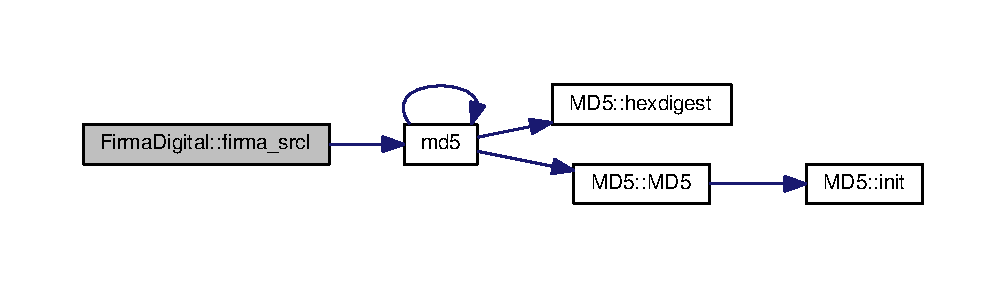
\includegraphics[width=350pt]{classFirmaDigital_ac68550394f9f4e0b73e80dc050875325_cgraph}
\end{center}
\end{figure}


\subsection{Documentación de los datos miembro}
\hypertarget{classFirmaDigital_a912b493f793c1e2ca268b534e65a65a0}{}\label{classFirmaDigital_a912b493f793c1e2ca268b534e65a65a0} 
\index{Firma\+Digital@{Firma\+Digital}!clave\+\_\+privada@{clave\+\_\+privada}}
\index{clave\+\_\+privada@{clave\+\_\+privada}!Firma\+Digital@{Firma\+Digital}}
\subsubsection{\texorpdfstring{clave\+\_\+privada}{clave\_privada}}
{\footnotesize\ttfamily string Firma\+Digital\+::clave\+\_\+privada}



clave\+\_\+privada 



Definición en la línea 30 del archivo Firma\+Digital.\+h.



La documentación para esta clase fue generada a partir de los siguientes ficheros\+:\begin{DoxyCompactItemize}
\item 
Template\+A\+F\+I\+S\+\_\+webservice\+\_\+lib/firma\+\_\+digital/\hyperlink{FirmaDigital_8h}{Firma\+Digital.\+h}\item 
Template\+A\+F\+I\+S\+\_\+webservice\+\_\+lib/firma\+\_\+digital/\hyperlink{FirmaDigital_8cpp}{Firma\+Digital.\+cpp}\end{DoxyCompactItemize}

\hypertarget{classGuiWsOpenErp}{}\section{Referencia de la Clase Gui\+Ws\+Open\+Erp}
\label{classGuiWsOpenErp}\index{Gui\+Ws\+Open\+Erp@{Gui\+Ws\+Open\+Erp}}


Clase que permite realizar la interacción con el Webservice con Open\+E\+RP. (No están en uso actualmente.)  


\subsection*{Métodos públicos}
\begin{DoxyCompactItemize}
\item 
\hyperlink{classGuiWsOpenErp_a468b3c76510469edce574ee3c2a86056}{Gui\+Ws\+Open\+Erp} (string \hyperlink{classGuiWsOpenErp_aa872d8ffb6c11032ec0dcfd8ee49e234}{dbname}, string \hyperlink{classGuiWsOpenErp_a34037b0900d58859cc4c42e77f170d82}{user}, string \hyperlink{classGuiWsOpenErp_ad82141631eb4a41cd62b1c8892424a92}{pwd}, string \hyperlink{classGuiWsOpenErp_a96c46b5aed53de6d0fca055f28862be5}{U\+RL})
\begin{DoxyCompactList}\small\item\em Constructor. \end{DoxyCompactList}\item 
\hyperlink{classGuiWsOpenErp_ac01e603d5d8486d9fef6f55b679cc8b6}{$\sim$\+Gui\+Ws\+Open\+Erp} ()
\begin{DoxyCompactList}\small\item\em Destructor. \end{DoxyCompactList}\item 
void \hyperlink{classGuiWsOpenErp_a72e93c46fcdf1317d7a554181f6e08e1}{Cargar\+Variables} (string \hyperlink{classGuiWsOpenErp_aa872d8ffb6c11032ec0dcfd8ee49e234}{dbname}, string \hyperlink{classGuiWsOpenErp_a34037b0900d58859cc4c42e77f170d82}{user}, string \hyperlink{classGuiWsOpenErp_ad82141631eb4a41cd62b1c8892424a92}{pwd}, string \hyperlink{classGuiWsOpenErp_a96c46b5aed53de6d0fca055f28862be5}{U\+RL})
\begin{DoxyCompactList}\small\item\em Cargar\+Variables Seteo de variables. \end{DoxyCompactList}\item 
long int \hyperlink{classGuiWsOpenErp_a48d629317e4b3be8b5471e5a14a60082}{Inicializar} ()
\begin{DoxyCompactList}\small\item\em Inicializar se encarga de la autentificacion contra el Open\+E\+RP. \end{DoxyCompactList}\item 
Xml\+Rpc\+Value \hyperlink{classGuiWsOpenErp_a417ed5728168fa74561efd022a42ae49}{Get\+Usuario} (string usuario)
\begin{DoxyCompactList}\small\item\em Get\+Usuario Este metodo se encarga de buscar en la tabla res.\+users parametrizado con la variable \char`\"{}usuario\char`\"{}. \end{DoxyCompactList}\item 
Xml\+Rpc\+Value \hyperlink{classGuiWsOpenErp_ae6d4fbf9fa54b3ab177f541dcb15b64f}{Get\+Dato\+Persona} (string cedula\+\_\+identidad)
\begin{DoxyCompactList}\small\item\em Get\+Dato\+Persona Este metodo se encarga de buscar en la tabla res.\+partner. \end{DoxyCompactList}\item 
Xml\+Rpc\+Value \hyperlink{classGuiWsOpenErp_aeb56055280e6dcceb9b3da722c20a5ce}{Get\+Persona\+By\+O\+B\+PP} (string situr\+\_\+code)
\begin{DoxyCompactList}\small\item\em Get\+Persona\+By\+O\+B\+PP Este metodo se encarga de buscar todas las personas a la cual pertene una obpp, para ello se parametriza la busquedad con el cdigo situr. \end{DoxyCompactList}\item 
Xml\+Rpc\+Value \hyperlink{classGuiWsOpenErp_ac8f72cfebf3c98364303d4851752fbf6}{Get\+Datoid\+Imagen} (long int partner\+\_\+id, string hand, string finger)
\begin{DoxyCompactList}\small\item\em Get\+Datoid\+Imagen Este metodo se encarga de obtener el id de un registro en la tabla res.\+partner.\+fingerprint para ello la busquedad es parametrizada con partner\+\_\+id, hand y finger. \end{DoxyCompactList}\item 
Xml\+Rpc\+Value \hyperlink{classGuiWsOpenErp_a128600b86f70773fb336c6b59c853b42}{get\+Dato\+Persona\+Verificacion} (string cedula)
\begin{DoxyCompactList}\small\item\em get\+Dato\+Persona\+Verificacion Este metodo se encarga de buscar los datos de la persona, a la cual se le verifica la huella. \end{DoxyCompactList}\item 
Xml\+Rpc\+Value \hyperlink{classGuiWsOpenErp_a331ff67a1bff59ac435a372fbd08b04b}{buscar\+Proyecto} (int id\+\_\+obpp)
\item 
Xml\+Rpc\+Value \hyperlink{classGuiWsOpenErp_a96d20089ae0aa7b9c262c23d66956274}{get\+Dato\+Huella} (string cedula, string \&mano, int \&dedo)
\begin{DoxyCompactList}\small\item\em get\+Dato\+Huella Este metodo se encarga de buscar las huellas que tiene registrado un integrante de la obpp, cuando se va a verificar. \end{DoxyCompactList}\end{DoxyCompactItemize}
\subsection*{Atributos privados}
\begin{DoxyCompactItemize}
\item 
string \hyperlink{classGuiWsOpenErp_aa872d8ffb6c11032ec0dcfd8ee49e234}{dbname}
\begin{DoxyCompactList}\small\item\em dbname \end{DoxyCompactList}\item 
string \hyperlink{classGuiWsOpenErp_a34037b0900d58859cc4c42e77f170d82}{user}
\begin{DoxyCompactList}\small\item\em user \end{DoxyCompactList}\item 
string \hyperlink{classGuiWsOpenErp_ad82141631eb4a41cd62b1c8892424a92}{pwd}
\begin{DoxyCompactList}\small\item\em pwd \end{DoxyCompactList}\item 
string \hyperlink{classGuiWsOpenErp_aa01da7bfce4fce442c869c6d1c988c4b}{model}
\begin{DoxyCompactList}\small\item\em U\+RL. \end{DoxyCompactList}\item 
string \hyperlink{classGuiWsOpenErp_a96c46b5aed53de6d0fca055f28862be5}{U\+RL}
\begin{DoxyCompactList}\small\item\em U\+RL. \end{DoxyCompactList}\item 
Xml\+Rpc\+Value\+::int32 \hyperlink{classGuiWsOpenErp_a791f1dd8b0b16f454ae7f1a2abe0a761}{uid}
\begin{DoxyCompactList}\small\item\em uid \end{DoxyCompactList}\end{DoxyCompactItemize}


\subsection{Descripción detallada}
Clase que permite realizar la interacción con el Webservice con Open\+E\+RP. (No están en uso actualmente.) 

Definición en la línea 39 del archivo Gui\+Ws\+Open\+Erp.\+cpp.



\subsection{Documentación del constructor y destructor}
\hypertarget{classGuiWsOpenErp_a468b3c76510469edce574ee3c2a86056}{}\label{classGuiWsOpenErp_a468b3c76510469edce574ee3c2a86056} 
\index{Gui\+Ws\+Open\+Erp@{Gui\+Ws\+Open\+Erp}!Gui\+Ws\+Open\+Erp@{Gui\+Ws\+Open\+Erp}}
\index{Gui\+Ws\+Open\+Erp@{Gui\+Ws\+Open\+Erp}!Gui\+Ws\+Open\+Erp@{Gui\+Ws\+Open\+Erp}}
\subsubsection{\texorpdfstring{Gui\+Ws\+Open\+Erp()}{GuiWsOpenErp()}}
{\footnotesize\ttfamily Gui\+Ws\+Open\+Erp\+::\+Gui\+Ws\+Open\+Erp (\begin{DoxyParamCaption}\item[{string}]{dbname,  }\item[{string}]{user,  }\item[{string}]{pwd,  }\item[{string}]{U\+RL }\end{DoxyParamCaption})\hspace{0.3cm}{\ttfamily [inline]}}



Constructor. 


\begin{DoxyParams}{Parámetros}
{\em dbname} & Nombre de la base de datos \\
\hline
{\em user} & Nombre de usuario \\
\hline
{\em pwd} & Contraseña de user \\
\hline
{\em U\+RL} & U\+RL \\
\hline
\end{DoxyParams}


Definición en la línea 73 del archivo Gui\+Ws\+Open\+Erp.\+cpp.

\hypertarget{classGuiWsOpenErp_ac01e603d5d8486d9fef6f55b679cc8b6}{}\label{classGuiWsOpenErp_ac01e603d5d8486d9fef6f55b679cc8b6} 
\index{Gui\+Ws\+Open\+Erp@{Gui\+Ws\+Open\+Erp}!````~Gui\+Ws\+Open\+Erp@{$\sim$\+Gui\+Ws\+Open\+Erp}}
\index{````~Gui\+Ws\+Open\+Erp@{$\sim$\+Gui\+Ws\+Open\+Erp}!Gui\+Ws\+Open\+Erp@{Gui\+Ws\+Open\+Erp}}
\subsubsection{\texorpdfstring{$\sim$\+Gui\+Ws\+Open\+Erp()}{~GuiWsOpenErp()}}
{\footnotesize\ttfamily Gui\+Ws\+Open\+Erp\+::$\sim$\+Gui\+Ws\+Open\+Erp (\begin{DoxyParamCaption}{ }\end{DoxyParamCaption})\hspace{0.3cm}{\ttfamily [inline]}}



Destructor. 



Definición en la línea 84 del archivo Gui\+Ws\+Open\+Erp.\+cpp.



\subsection{Documentación de las funciones miembro}
\hypertarget{classGuiWsOpenErp_a331ff67a1bff59ac435a372fbd08b04b}{}\label{classGuiWsOpenErp_a331ff67a1bff59ac435a372fbd08b04b} 
\index{Gui\+Ws\+Open\+Erp@{Gui\+Ws\+Open\+Erp}!buscar\+Proyecto@{buscar\+Proyecto}}
\index{buscar\+Proyecto@{buscar\+Proyecto}!Gui\+Ws\+Open\+Erp@{Gui\+Ws\+Open\+Erp}}
\subsubsection{\texorpdfstring{buscar\+Proyecto()}{buscarProyecto()}}
{\footnotesize\ttfamily Xml\+Rpc\+Value Gui\+Ws\+Open\+Erp\+::buscar\+Proyecto (\begin{DoxyParamCaption}\item[{int}]{id\+\_\+obpp }\end{DoxyParamCaption})\hspace{0.3cm}{\ttfamily [inline]}}



Definición en la línea 645 del archivo Gui\+Ws\+Open\+Erp.\+cpp.

\hypertarget{classGuiWsOpenErp_a72e93c46fcdf1317d7a554181f6e08e1}{}\label{classGuiWsOpenErp_a72e93c46fcdf1317d7a554181f6e08e1} 
\index{Gui\+Ws\+Open\+Erp@{Gui\+Ws\+Open\+Erp}!Cargar\+Variables@{Cargar\+Variables}}
\index{Cargar\+Variables@{Cargar\+Variables}!Gui\+Ws\+Open\+Erp@{Gui\+Ws\+Open\+Erp}}
\subsubsection{\texorpdfstring{Cargar\+Variables()}{CargarVariables()}}
{\footnotesize\ttfamily void Gui\+Ws\+Open\+Erp\+::\+Cargar\+Variables (\begin{DoxyParamCaption}\item[{string}]{dbname,  }\item[{string}]{user,  }\item[{string}]{pwd,  }\item[{string}]{U\+RL }\end{DoxyParamCaption})\hspace{0.3cm}{\ttfamily [inline]}}



Cargar\+Variables Seteo de variables. 


\begin{DoxyParams}{Parámetros}
{\em dbname} & \\
\hline
{\em user} & \\
\hline
{\em pwd} & \\
\hline
{\em U\+RL} & \\
\hline
\end{DoxyParams}


Definición en la línea 95 del archivo Gui\+Ws\+Open\+Erp.\+cpp.

\hypertarget{classGuiWsOpenErp_a96d20089ae0aa7b9c262c23d66956274}{}\label{classGuiWsOpenErp_a96d20089ae0aa7b9c262c23d66956274} 
\index{Gui\+Ws\+Open\+Erp@{Gui\+Ws\+Open\+Erp}!get\+Dato\+Huella@{get\+Dato\+Huella}}
\index{get\+Dato\+Huella@{get\+Dato\+Huella}!Gui\+Ws\+Open\+Erp@{Gui\+Ws\+Open\+Erp}}
\subsubsection{\texorpdfstring{get\+Dato\+Huella()}{getDatoHuella()}}
{\footnotesize\ttfamily Xml\+Rpc\+Value Gui\+Ws\+Open\+Erp\+::get\+Dato\+Huella (\begin{DoxyParamCaption}\item[{string}]{cedula,  }\item[{string \&}]{mano,  }\item[{int \&}]{dedo }\end{DoxyParamCaption})\hspace{0.3cm}{\ttfamily [inline]}}



get\+Dato\+Huella Este metodo se encarga de buscar las huellas que tiene registrado un integrante de la obpp, cuando se va a verificar. 


\begin{DoxyParams}{Parámetros}
{\em cedula} & \\
\hline
{\em mano} & \\
\hline
{\em dedo} & \\
\hline
\end{DoxyParams}
\begin{DoxyReturn}{Devuelve}
Retorna mano y dedo por referencia. Y datos de la Huella por Xml\+Rpc\+Value 
\end{DoxyReturn}


Definición en la línea 697 del archivo Gui\+Ws\+Open\+Erp.\+cpp.



Referenciado por Template\+A\+F\+I\+S\+\_\+webservice\+::get\+Datos\+Huella().

\hypertarget{classGuiWsOpenErp_ac8f72cfebf3c98364303d4851752fbf6}{}\label{classGuiWsOpenErp_ac8f72cfebf3c98364303d4851752fbf6} 
\index{Gui\+Ws\+Open\+Erp@{Gui\+Ws\+Open\+Erp}!Get\+Datoid\+Imagen@{Get\+Datoid\+Imagen}}
\index{Get\+Datoid\+Imagen@{Get\+Datoid\+Imagen}!Gui\+Ws\+Open\+Erp@{Gui\+Ws\+Open\+Erp}}
\subsubsection{\texorpdfstring{Get\+Datoid\+Imagen()}{GetDatoidImagen()}}
{\footnotesize\ttfamily Xml\+Rpc\+Value Gui\+Ws\+Open\+Erp\+::\+Get\+Datoid\+Imagen (\begin{DoxyParamCaption}\item[{long int}]{partner\+\_\+id,  }\item[{string}]{hand,  }\item[{string}]{finger }\end{DoxyParamCaption})\hspace{0.3cm}{\ttfamily [inline]}}



Get\+Datoid\+Imagen Este metodo se encarga de obtener el id de un registro en la tabla res.\+partner.\+fingerprint para ello la busquedad es parametrizada con partner\+\_\+id, hand y finger. 


\begin{DoxyParams}{Parámetros}
{\em partner\+\_\+id} & Viene de la G\+UI \\
\hline
{\em hand} & Viene de la G\+UI \\
\hline
{\em finger} & Viene de la G\+UI \\
\hline
\end{DoxyParams}
\begin{DoxyReturn}{Devuelve}
result\+\_\+read es un struct Xml\+Rpc\+Value 
\end{DoxyReturn}


Definición en la línea 398 del archivo Gui\+Ws\+Open\+Erp.\+cpp.

\hypertarget{classGuiWsOpenErp_ae6d4fbf9fa54b3ab177f541dcb15b64f}{}\label{classGuiWsOpenErp_ae6d4fbf9fa54b3ab177f541dcb15b64f} 
\index{Gui\+Ws\+Open\+Erp@{Gui\+Ws\+Open\+Erp}!Get\+Dato\+Persona@{Get\+Dato\+Persona}}
\index{Get\+Dato\+Persona@{Get\+Dato\+Persona}!Gui\+Ws\+Open\+Erp@{Gui\+Ws\+Open\+Erp}}
\subsubsection{\texorpdfstring{Get\+Dato\+Persona()}{GetDatoPersona()}}
{\footnotesize\ttfamily Xml\+Rpc\+Value Gui\+Ws\+Open\+Erp\+::\+Get\+Dato\+Persona (\begin{DoxyParamCaption}\item[{string}]{cedula\+\_\+identidad }\end{DoxyParamCaption})\hspace{0.3cm}{\ttfamily [inline]}}



Get\+Dato\+Persona Este metodo se encarga de buscar en la tabla res.\+partner. 


\begin{DoxyParams}{Parámetros}
{\em cedula\+\_\+identidad} & Viene de la G\+UI \\
\hline
\end{DoxyParams}
\begin{DoxyReturn}{Devuelve}
identification\+\_\+id \& name. 
\end{DoxyReturn}


Definición en la línea 189 del archivo Gui\+Ws\+Open\+Erp.\+cpp.



Referenciado por Template\+A\+F\+I\+S\+\_\+webservice\+::get\+Datos\+Persona().

\hypertarget{classGuiWsOpenErp_a128600b86f70773fb336c6b59c853b42}{}\label{classGuiWsOpenErp_a128600b86f70773fb336c6b59c853b42} 
\index{Gui\+Ws\+Open\+Erp@{Gui\+Ws\+Open\+Erp}!get\+Dato\+Persona\+Verificacion@{get\+Dato\+Persona\+Verificacion}}
\index{get\+Dato\+Persona\+Verificacion@{get\+Dato\+Persona\+Verificacion}!Gui\+Ws\+Open\+Erp@{Gui\+Ws\+Open\+Erp}}
\subsubsection{\texorpdfstring{get\+Dato\+Persona\+Verificacion()}{getDatoPersonaVerificacion()}}
{\footnotesize\ttfamily Xml\+Rpc\+Value Gui\+Ws\+Open\+Erp\+::get\+Dato\+Persona\+Verificacion (\begin{DoxyParamCaption}\item[{string}]{cedula }\end{DoxyParamCaption})\hspace{0.3cm}{\ttfamily [inline]}}



get\+Dato\+Persona\+Verificacion Este metodo se encarga de buscar los datos de la persona, a la cual se le verifica la huella. 


\begin{DoxyParams}{Parámetros}
{\em cedula} & Viene de la G\+UI \\
\hline
\end{DoxyParams}
\begin{DoxyReturn}{Devuelve}
Datos de verificación para una persona 
\end{DoxyReturn}


Definición en la línea 467 del archivo Gui\+Ws\+Open\+Erp.\+cpp.



Referenciado por Template\+A\+F\+I\+S\+\_\+webservice\+::get\+Datos\+Persona\+Verificacion().

\hypertarget{classGuiWsOpenErp_aeb56055280e6dcceb9b3da722c20a5ce}{}\label{classGuiWsOpenErp_aeb56055280e6dcceb9b3da722c20a5ce} 
\index{Gui\+Ws\+Open\+Erp@{Gui\+Ws\+Open\+Erp}!Get\+Persona\+By\+O\+B\+PP@{Get\+Persona\+By\+O\+B\+PP}}
\index{Get\+Persona\+By\+O\+B\+PP@{Get\+Persona\+By\+O\+B\+PP}!Gui\+Ws\+Open\+Erp@{Gui\+Ws\+Open\+Erp}}
\subsubsection{\texorpdfstring{Get\+Persona\+By\+O\+B\+P\+P()}{GetPersonaByOBPP()}}
{\footnotesize\ttfamily Xml\+Rpc\+Value Gui\+Ws\+Open\+Erp\+::\+Get\+Persona\+By\+O\+B\+PP (\begin{DoxyParamCaption}\item[{string}]{situr\+\_\+code }\end{DoxyParamCaption})\hspace{0.3cm}{\ttfamily [inline]}}



Get\+Persona\+By\+O\+B\+PP Este metodo se encarga de buscar todas las personas a la cual pertene una obpp, para ello se parametriza la busquedad con el cdigo situr. 


\begin{DoxyParams}{Parámetros}
{\em situr\+\_\+code} & Viene de la G\+UI \\
\hline
\end{DoxyParams}
\begin{DoxyReturn}{Devuelve}
Valores de la O\+B\+PP 
\end{DoxyReturn}


Definición en la línea 246 del archivo Gui\+Ws\+Open\+Erp.\+cpp.



Hace referencia a N\+A\+ME y V\+E\+R\+S\+I\+ON.



Referenciado por Template\+A\+F\+I\+S\+\_\+webservice\+::get\+Datos\+Persona\+O\+B\+P\+P().

\hypertarget{classGuiWsOpenErp_a417ed5728168fa74561efd022a42ae49}{}\label{classGuiWsOpenErp_a417ed5728168fa74561efd022a42ae49} 
\index{Gui\+Ws\+Open\+Erp@{Gui\+Ws\+Open\+Erp}!Get\+Usuario@{Get\+Usuario}}
\index{Get\+Usuario@{Get\+Usuario}!Gui\+Ws\+Open\+Erp@{Gui\+Ws\+Open\+Erp}}
\subsubsection{\texorpdfstring{Get\+Usuario()}{GetUsuario()}}
{\footnotesize\ttfamily Xml\+Rpc\+Value Gui\+Ws\+Open\+Erp\+::\+Get\+Usuario (\begin{DoxyParamCaption}\item[{string}]{usuario }\end{DoxyParamCaption})\hspace{0.3cm}{\ttfamily [inline]}}



Get\+Usuario Este metodo se encarga de buscar en la tabla res.\+users parametrizado con la variable \char`\"{}usuario\char`\"{}. 


\begin{DoxyParams}{Parámetros}
{\em usuario} & Viene de la G\+UI \\
\hline
\end{DoxyParams}
\begin{DoxyReturn}{Devuelve}
id \& login. 
\end{DoxyReturn}


Definición en la línea 131 del archivo Gui\+Ws\+Open\+Erp.\+cpp.

\hypertarget{classGuiWsOpenErp_a48d629317e4b3be8b5471e5a14a60082}{}\label{classGuiWsOpenErp_a48d629317e4b3be8b5471e5a14a60082} 
\index{Gui\+Ws\+Open\+Erp@{Gui\+Ws\+Open\+Erp}!Inicializar@{Inicializar}}
\index{Inicializar@{Inicializar}!Gui\+Ws\+Open\+Erp@{Gui\+Ws\+Open\+Erp}}
\subsubsection{\texorpdfstring{Inicializar()}{Inicializar()}}
{\footnotesize\ttfamily long int Gui\+Ws\+Open\+Erp\+::\+Inicializar (\begin{DoxyParamCaption}{ }\end{DoxyParamCaption})\hspace{0.3cm}{\ttfamily [inline]}}



Inicializar se encarga de la autentificacion contra el Open\+E\+RP. 

\begin{DoxyReturn}{Devuelve}
el id del usuario que se autentifica. 
\end{DoxyReturn}


Definición en la línea 107 del archivo Gui\+Ws\+Open\+Erp.\+cpp.



Hace referencia a N\+A\+ME y V\+E\+R\+S\+I\+ON.



Referenciado por Template\+A\+F\+I\+S\+\_\+webservice\+::comprobar(), Template\+A\+F\+I\+S\+\_\+webservice\+::get\+Datos\+Huella(), Template\+A\+F\+I\+S\+\_\+webservice\+::get\+Datos\+Persona(), Template\+A\+F\+I\+S\+\_\+webservice\+::get\+Datos\+Persona\+O\+B\+P\+P(), Template\+A\+F\+I\+S\+\_\+webservice\+::get\+Datos\+Persona\+Verificacion() y Template\+A\+F\+I\+S\+\_\+webservice\+::get\+Usuario().



\subsection{Documentación de los datos miembro}
\hypertarget{classGuiWsOpenErp_aa872d8ffb6c11032ec0dcfd8ee49e234}{}\label{classGuiWsOpenErp_aa872d8ffb6c11032ec0dcfd8ee49e234} 
\index{Gui\+Ws\+Open\+Erp@{Gui\+Ws\+Open\+Erp}!dbname@{dbname}}
\index{dbname@{dbname}!Gui\+Ws\+Open\+Erp@{Gui\+Ws\+Open\+Erp}}
\subsubsection{\texorpdfstring{dbname}{dbname}}
{\footnotesize\ttfamily string Gui\+Ws\+Open\+Erp\+::dbname\hspace{0.3cm}{\ttfamily [private]}}



dbname 



Definición en la línea 43 del archivo Gui\+Ws\+Open\+Erp.\+cpp.

\hypertarget{classGuiWsOpenErp_aa01da7bfce4fce442c869c6d1c988c4b}{}\label{classGuiWsOpenErp_aa01da7bfce4fce442c869c6d1c988c4b} 
\index{Gui\+Ws\+Open\+Erp@{Gui\+Ws\+Open\+Erp}!model@{model}}
\index{model@{model}!Gui\+Ws\+Open\+Erp@{Gui\+Ws\+Open\+Erp}}
\subsubsection{\texorpdfstring{model}{model}}
{\footnotesize\ttfamily string Gui\+Ws\+Open\+Erp\+::model\hspace{0.3cm}{\ttfamily [private]}}



U\+RL. 



Definición en la línea 55 del archivo Gui\+Ws\+Open\+Erp.\+cpp.

\hypertarget{classGuiWsOpenErp_ad82141631eb4a41cd62b1c8892424a92}{}\label{classGuiWsOpenErp_ad82141631eb4a41cd62b1c8892424a92} 
\index{Gui\+Ws\+Open\+Erp@{Gui\+Ws\+Open\+Erp}!pwd@{pwd}}
\index{pwd@{pwd}!Gui\+Ws\+Open\+Erp@{Gui\+Ws\+Open\+Erp}}
\subsubsection{\texorpdfstring{pwd}{pwd}}
{\footnotesize\ttfamily string Gui\+Ws\+Open\+Erp\+::pwd\hspace{0.3cm}{\ttfamily [private]}}



pwd 



Definición en la línea 51 del archivo Gui\+Ws\+Open\+Erp.\+cpp.

\hypertarget{classGuiWsOpenErp_a791f1dd8b0b16f454ae7f1a2abe0a761}{}\label{classGuiWsOpenErp_a791f1dd8b0b16f454ae7f1a2abe0a761} 
\index{Gui\+Ws\+Open\+Erp@{Gui\+Ws\+Open\+Erp}!uid@{uid}}
\index{uid@{uid}!Gui\+Ws\+Open\+Erp@{Gui\+Ws\+Open\+Erp}}
\subsubsection{\texorpdfstring{uid}{uid}}
{\footnotesize\ttfamily Xml\+Rpc\+Value\+::int32 Gui\+Ws\+Open\+Erp\+::uid\hspace{0.3cm}{\ttfamily [private]}}



uid 



Definición en la línea 63 del archivo Gui\+Ws\+Open\+Erp.\+cpp.

\hypertarget{classGuiWsOpenErp_a96c46b5aed53de6d0fca055f28862be5}{}\label{classGuiWsOpenErp_a96c46b5aed53de6d0fca055f28862be5} 
\index{Gui\+Ws\+Open\+Erp@{Gui\+Ws\+Open\+Erp}!U\+RL@{U\+RL}}
\index{U\+RL@{U\+RL}!Gui\+Ws\+Open\+Erp@{Gui\+Ws\+Open\+Erp}}
\subsubsection{\texorpdfstring{U\+RL}{URL}}
{\footnotesize\ttfamily string Gui\+Ws\+Open\+Erp\+::\+U\+RL\hspace{0.3cm}{\ttfamily [private]}}



U\+RL. 



Definición en la línea 59 del archivo Gui\+Ws\+Open\+Erp.\+cpp.

\hypertarget{classGuiWsOpenErp_a34037b0900d58859cc4c42e77f170d82}{}\label{classGuiWsOpenErp_a34037b0900d58859cc4c42e77f170d82} 
\index{Gui\+Ws\+Open\+Erp@{Gui\+Ws\+Open\+Erp}!user@{user}}
\index{user@{user}!Gui\+Ws\+Open\+Erp@{Gui\+Ws\+Open\+Erp}}
\subsubsection{\texorpdfstring{user}{user}}
{\footnotesize\ttfamily string Gui\+Ws\+Open\+Erp\+::user\hspace{0.3cm}{\ttfamily [private]}}



user 



Definición en la línea 47 del archivo Gui\+Ws\+Open\+Erp.\+cpp.



La documentación para esta clase fue generada a partir del siguiente fichero\+:\begin{DoxyCompactItemize}
\item 
Template\+A\+F\+I\+S\+\_\+webservice\+\_\+lib/\+Conexion\+\_\+webservice/\hyperlink{GuiWsOpenErp_8cpp}{Gui\+Ws\+Open\+Erp.\+cpp}\end{DoxyCompactItemize}

\hypertarget{classImagen}{}\section{Referencia de la Clase Imagen}
\label{classImagen}\index{Imagen@{Imagen}}


Clase \hyperlink{classImagen}{Imagen}\+: Almacena las imágenes y variables.  




{\ttfamily \#include $<$Template\+A\+F\+I\+S.\+h$>$}

\subsection*{Métodos públicos}
\begin{DoxyCompactItemize}
\item 
\hyperlink{classImagen_a806163aa3eaf4022030a49275ddf4d2b}{Imagen} (string \hyperlink{classImagen_a92940ae8127167d1a7041a365555a931}{id}, unsigned char $\ast$\hyperlink{classImagen_a8485fa6dd60a7f067e2d2066599314b0}{imagen}, int \hyperlink{classImagen_a7b9235e12e5cc50f29614e9c08d72c4f}{n\+Width}, int \hyperlink{classImagen_a92935096f7cbcc6ffe32dde43038288c}{n\+Height}, long int \hyperlink{classImagen_adb26157b4817c521f092f024d28b9435}{n\+Size}, string \hyperlink{classImagen_aef38d4f4f82b0f19b4b13b20d66e38ba}{id\+\_\+persona}, string \hyperlink{classImagen_abdf777e9a6d41cb3b6ee54e9702d0e52}{id\+\_\+dedo}, string \hyperlink{classImagen_a6ac88dc4f15daed005f1055235020821}{mano})
\begin{DoxyCompactList}\small\item\em Constructor. \end{DoxyCompactList}\item 
\hyperlink{classImagen_a03dd93c9cf920a9dc0b72f8bd34f2e8a}{$\sim$\+Imagen} ()
\begin{DoxyCompactList}\small\item\em Destructor. \end{DoxyCompactList}\item 
unsigned char $\ast$ \hyperlink{classImagen_a676804752c281116609460f738b74924}{get\+Imagen} (unsigned char $\ast$\&\hyperlink{classImagen_a8485fa6dd60a7f067e2d2066599314b0}{imagen})
\begin{DoxyCompactList}\small\item\em Get \hyperlink{classImagen}{Imagen}. \end{DoxyCompactList}\item 
int \hyperlink{classImagen_a4f973d4f8e63503c3e0b4649a95e0188}{get\+Width} ()
\begin{DoxyCompactList}\small\item\em Get Width. \end{DoxyCompactList}\item 
int \hyperlink{classImagen_a1f243282c3f962c9694b53bc9106215b}{get\+Height} ()
\begin{DoxyCompactList}\small\item\em Get Height. \end{DoxyCompactList}\item 
long int \hyperlink{classImagen_afa3177842fed7750c8c51eeeaf108adb}{get\+Size} ()
\begin{DoxyCompactList}\small\item\em Get Size. \end{DoxyCompactList}\item 
string \hyperlink{classImagen_a4cac81ed0243f264dcbaae552b936038}{get\+Id} ()
\begin{DoxyCompactList}\small\item\em Get Id. \end{DoxyCompactList}\item 
string \hyperlink{classImagen_a6fe8c566e03b1c6e2d6818b1886ad522}{get\+Id\+Persona} ()
\begin{DoxyCompactList}\small\item\em Get Id Persona. \end{DoxyCompactList}\item 
string \hyperlink{classImagen_af8f9c814f372583821f412e2475e9fda}{get\+Id\+Dedo} ()
\begin{DoxyCompactList}\small\item\em Get Id Persona. \end{DoxyCompactList}\item 
string \hyperlink{classImagen_a687160f46f2e80fee30dac0955268c39}{get\+Mano} ()
\begin{DoxyCompactList}\small\item\em Get Id Persona. \end{DoxyCompactList}\item 
long int \hyperlink{classImagen_afae009c9516b1d67bf7aca237f6ef403}{sizeof\+Object} ()
\begin{DoxyCompactList}\small\item\em Get Id Persona. \end{DoxyCompactList}\end{DoxyCompactItemize}
\subsection*{Atributos públicos}
\begin{DoxyCompactItemize}
\item 
unsigned char $\ast$ \hyperlink{classImagen_a8485fa6dd60a7f067e2d2066599314b0}{imagen}
\begin{DoxyCompactList}\small\item\em imagen \end{DoxyCompactList}\item 
int \hyperlink{classImagen_a7b9235e12e5cc50f29614e9c08d72c4f}{n\+Width}
\begin{DoxyCompactList}\small\item\em n\+Width \end{DoxyCompactList}\item 
int \hyperlink{classImagen_a92935096f7cbcc6ffe32dde43038288c}{n\+Height}
\begin{DoxyCompactList}\small\item\em n\+Height \end{DoxyCompactList}\item 
long int \hyperlink{classImagen_adb26157b4817c521f092f024d28b9435}{n\+Size}
\begin{DoxyCompactList}\small\item\em n\+Size \end{DoxyCompactList}\item 
string \hyperlink{classImagen_a92940ae8127167d1a7041a365555a931}{id}
\begin{DoxyCompactList}\small\item\em id \end{DoxyCompactList}\item 
string \hyperlink{classImagen_aef38d4f4f82b0f19b4b13b20d66e38ba}{id\+\_\+persona}
\begin{DoxyCompactList}\small\item\em id\+\_\+persona \end{DoxyCompactList}\item 
string \hyperlink{classImagen_abdf777e9a6d41cb3b6ee54e9702d0e52}{id\+\_\+dedo}
\begin{DoxyCompactList}\small\item\em id\+\_\+dedo \end{DoxyCompactList}\item 
string \hyperlink{classImagen_a6ac88dc4f15daed005f1055235020821}{mano}
\begin{DoxyCompactList}\small\item\em mano \end{DoxyCompactList}\end{DoxyCompactItemize}


\subsection{Descripción detallada}
Clase \hyperlink{classImagen}{Imagen}\+: Almacena las imágenes y variables. 

Definición en la línea 96 del archivo Template\+A\+F\+I\+S.\+h.



\subsection{Documentación del constructor y destructor}
\hypertarget{classImagen_a806163aa3eaf4022030a49275ddf4d2b}{}\label{classImagen_a806163aa3eaf4022030a49275ddf4d2b} 
\index{Imagen@{Imagen}!Imagen@{Imagen}}
\index{Imagen@{Imagen}!Imagen@{Imagen}}
\subsubsection{\texorpdfstring{Imagen()}{Imagen()}}
{\footnotesize\ttfamily Imagen\+::\+Imagen (\begin{DoxyParamCaption}\item[{string}]{id,  }\item[{unsigned char $\ast$}]{imagen,  }\item[{int}]{n\+Width,  }\item[{int}]{n\+Height,  }\item[{long int}]{n\+Size,  }\item[{string}]{id\+\_\+persona,  }\item[{string}]{id\+\_\+dedo,  }\item[{string}]{mano }\end{DoxyParamCaption})}



Constructor. 

Clase \hyperlink{classImagen}{Imagen}\+: Almacena las imágenes y variables. Almacena en memoria las imágenes para que puedan ser manipuladas por el webservice. 

Definición en la línea 20 del archivo Template\+A\+F\+I\+S.\+cpp.



Hace referencia a id, id\+\_\+dedo, id\+\_\+persona, imagen, mano, n\+Height, n\+Size y n\+Width.

\hypertarget{classImagen_a03dd93c9cf920a9dc0b72f8bd34f2e8a}{}\label{classImagen_a03dd93c9cf920a9dc0b72f8bd34f2e8a} 
\index{Imagen@{Imagen}!````~Imagen@{$\sim$\+Imagen}}
\index{````~Imagen@{$\sim$\+Imagen}!Imagen@{Imagen}}
\subsubsection{\texorpdfstring{$\sim$\+Imagen()}{~Imagen()}}
{\footnotesize\ttfamily Imagen\+::$\sim$\+Imagen (\begin{DoxyParamCaption}{ }\end{DoxyParamCaption})}



Destructor. 



Definición en la línea 33 del archivo Template\+A\+F\+I\+S.\+cpp.



\subsection{Documentación de las funciones miembro}
\hypertarget{classImagen_a1f243282c3f962c9694b53bc9106215b}{}\label{classImagen_a1f243282c3f962c9694b53bc9106215b} 
\index{Imagen@{Imagen}!get\+Height@{get\+Height}}
\index{get\+Height@{get\+Height}!Imagen@{Imagen}}
\subsubsection{\texorpdfstring{get\+Height()}{getHeight()}}
{\footnotesize\ttfamily int Imagen\+::get\+Height (\begin{DoxyParamCaption}{ }\end{DoxyParamCaption})}



Get Height. 

\begin{DoxyReturn}{Devuelve}
Obtiene alto de la imágen. 
\end{DoxyReturn}


Definición en la línea 47 del archivo Template\+A\+F\+I\+S.\+cpp.



Hace referencia a n\+Height.

\hypertarget{classImagen_a4cac81ed0243f264dcbaae552b936038}{}\label{classImagen_a4cac81ed0243f264dcbaae552b936038} 
\index{Imagen@{Imagen}!get\+Id@{get\+Id}}
\index{get\+Id@{get\+Id}!Imagen@{Imagen}}
\subsubsection{\texorpdfstring{get\+Id()}{getId()}}
{\footnotesize\ttfamily string Imagen\+::get\+Id (\begin{DoxyParamCaption}{ }\end{DoxyParamCaption})}



Get Id. 

\begin{DoxyReturn}{Devuelve}
Obtiene Id de la imágen en la Base de Datos. 
\end{DoxyReturn}


Definición en la línea 57 del archivo Template\+A\+F\+I\+S.\+cpp.



Hace referencia a id.

\hypertarget{classImagen_af8f9c814f372583821f412e2475e9fda}{}\label{classImagen_af8f9c814f372583821f412e2475e9fda} 
\index{Imagen@{Imagen}!get\+Id\+Dedo@{get\+Id\+Dedo}}
\index{get\+Id\+Dedo@{get\+Id\+Dedo}!Imagen@{Imagen}}
\subsubsection{\texorpdfstring{get\+Id\+Dedo()}{getIdDedo()}}
{\footnotesize\ttfamily string Imagen\+::get\+Id\+Dedo (\begin{DoxyParamCaption}{ }\end{DoxyParamCaption})}



Get Id Persona. 

\begin{DoxyReturn}{Devuelve}
Obtiene Id del dedo asociado a la imágen en la Base de Datos. 
\end{DoxyReturn}


Definición en la línea 67 del archivo Template\+A\+F\+I\+S.\+cpp.



Hace referencia a id\+\_\+dedo.

\hypertarget{classImagen_a6fe8c566e03b1c6e2d6818b1886ad522}{}\label{classImagen_a6fe8c566e03b1c6e2d6818b1886ad522} 
\index{Imagen@{Imagen}!get\+Id\+Persona@{get\+Id\+Persona}}
\index{get\+Id\+Persona@{get\+Id\+Persona}!Imagen@{Imagen}}
\subsubsection{\texorpdfstring{get\+Id\+Persona()}{getIdPersona()}}
{\footnotesize\ttfamily string Imagen\+::get\+Id\+Persona (\begin{DoxyParamCaption}{ }\end{DoxyParamCaption})}



Get Id Persona. 

\begin{DoxyReturn}{Devuelve}
Obtiene Id de la persona asociada a la imágen en la Base de Datos. 
\end{DoxyReturn}


Definición en la línea 62 del archivo Template\+A\+F\+I\+S.\+cpp.



Hace referencia a id\+\_\+persona.

\hypertarget{classImagen_a676804752c281116609460f738b74924}{}\label{classImagen_a676804752c281116609460f738b74924} 
\index{Imagen@{Imagen}!get\+Imagen@{get\+Imagen}}
\index{get\+Imagen@{get\+Imagen}!Imagen@{Imagen}}
\subsubsection{\texorpdfstring{get\+Imagen()}{getImagen()}}
{\footnotesize\ttfamily unsigned char $\ast$ Imagen\+::get\+Imagen (\begin{DoxyParamCaption}\item[{unsigned char $\ast$\&}]{imagen }\end{DoxyParamCaption})}



Get \hyperlink{classImagen}{Imagen}. 


\begin{DoxyParams}{Parámetros}
{\em imagen} & Una imágen cualquiera (parámetro de prueba) \\
\hline
\end{DoxyParams}
\begin{DoxyReturn}{Devuelve}
Obtiene la imágen. Este es el resultado. 
\end{DoxyReturn}


Definición en la línea 37 del archivo Template\+A\+F\+I\+S.\+cpp.



Hace referencia a imagen.

\hypertarget{classImagen_a687160f46f2e80fee30dac0955268c39}{}\label{classImagen_a687160f46f2e80fee30dac0955268c39} 
\index{Imagen@{Imagen}!get\+Mano@{get\+Mano}}
\index{get\+Mano@{get\+Mano}!Imagen@{Imagen}}
\subsubsection{\texorpdfstring{get\+Mano()}{getMano()}}
{\footnotesize\ttfamily string Imagen\+::get\+Mano (\begin{DoxyParamCaption}{ }\end{DoxyParamCaption})}



Get Id Persona. 

\begin{DoxyReturn}{Devuelve}
Obtiene mano asociada a la imágen en la Base de Datos. 
\end{DoxyReturn}


Definición en la línea 72 del archivo Template\+A\+F\+I\+S.\+cpp.



Hace referencia a mano.

\hypertarget{classImagen_afa3177842fed7750c8c51eeeaf108adb}{}\label{classImagen_afa3177842fed7750c8c51eeeaf108adb} 
\index{Imagen@{Imagen}!get\+Size@{get\+Size}}
\index{get\+Size@{get\+Size}!Imagen@{Imagen}}
\subsubsection{\texorpdfstring{get\+Size()}{getSize()}}
{\footnotesize\ttfamily long int Imagen\+::get\+Size (\begin{DoxyParamCaption}{ }\end{DoxyParamCaption})}



Get Size. 

\begin{DoxyReturn}{Devuelve}
Obtiene tamaño de la imágen. 
\end{DoxyReturn}


Definición en la línea 52 del archivo Template\+A\+F\+I\+S.\+cpp.



Hace referencia a n\+Size.



Referenciado por sizeof\+Object().

\hypertarget{classImagen_a4f973d4f8e63503c3e0b4649a95e0188}{}\label{classImagen_a4f973d4f8e63503c3e0b4649a95e0188} 
\index{Imagen@{Imagen}!get\+Width@{get\+Width}}
\index{get\+Width@{get\+Width}!Imagen@{Imagen}}
\subsubsection{\texorpdfstring{get\+Width()}{getWidth()}}
{\footnotesize\ttfamily int Imagen\+::get\+Width (\begin{DoxyParamCaption}{ }\end{DoxyParamCaption})}



Get Width. 

\begin{DoxyReturn}{Devuelve}
Obtiene ancho de la imágen. 
\end{DoxyReturn}


Definición en la línea 42 del archivo Template\+A\+F\+I\+S.\+cpp.



Hace referencia a n\+Width.

\hypertarget{classImagen_afae009c9516b1d67bf7aca237f6ef403}{}\label{classImagen_afae009c9516b1d67bf7aca237f6ef403} 
\index{Imagen@{Imagen}!sizeof\+Object@{sizeof\+Object}}
\index{sizeof\+Object@{sizeof\+Object}!Imagen@{Imagen}}
\subsubsection{\texorpdfstring{sizeof\+Object()}{sizeofObject()}}
{\footnotesize\ttfamily long int Imagen\+::sizeof\+Object (\begin{DoxyParamCaption}{ }\end{DoxyParamCaption})}



Get Id Persona. 

\begin{DoxyReturn}{Devuelve}
Obtiene el tamaño del objeto \hyperlink{classImagen}{Imagen}. 
\end{DoxyReturn}


Definición en la línea 77 del archivo Template\+A\+F\+I\+S.\+cpp.



Hace referencia a get\+Size(), id\+\_\+dedo, id\+\_\+persona, mano, n\+Height, n\+Size y n\+Width.

Gráfico de llamadas para esta función\+:\nopagebreak
\begin{figure}[H]
\begin{center}
\leavevmode
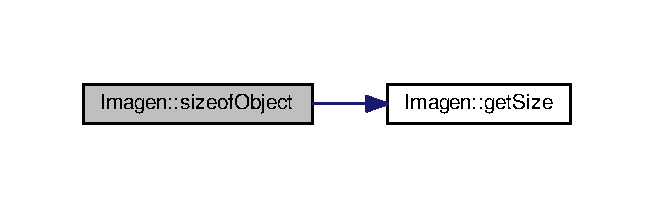
\includegraphics[width=314pt]{classImagen_afae009c9516b1d67bf7aca237f6ef403_cgraph}
\end{center}
\end{figure}


\subsection{Documentación de los datos miembro}
\hypertarget{classImagen_a92940ae8127167d1a7041a365555a931}{}\label{classImagen_a92940ae8127167d1a7041a365555a931} 
\index{Imagen@{Imagen}!id@{id}}
\index{id@{id}!Imagen@{Imagen}}
\subsubsection{\texorpdfstring{id}{id}}
{\footnotesize\ttfamily string Imagen\+::id}



id 



Definición en la línea 118 del archivo Template\+A\+F\+I\+S.\+h.



Referenciado por get\+Id(), Imagen() y Template\+A\+F\+I\+S\+\_\+webservice\+::salvar\+J\+P\+E\+G().

\hypertarget{classImagen_abdf777e9a6d41cb3b6ee54e9702d0e52}{}\label{classImagen_abdf777e9a6d41cb3b6ee54e9702d0e52} 
\index{Imagen@{Imagen}!id\+\_\+dedo@{id\+\_\+dedo}}
\index{id\+\_\+dedo@{id\+\_\+dedo}!Imagen@{Imagen}}
\subsubsection{\texorpdfstring{id\+\_\+dedo}{id\_dedo}}
{\footnotesize\ttfamily string Imagen\+::id\+\_\+dedo}



id\+\_\+dedo 



Definición en la línea 126 del archivo Template\+A\+F\+I\+S.\+h.



Referenciado por get\+Id\+Dedo(), Imagen(), Template\+A\+F\+I\+S\+\_\+webservice\+::\+On\+Identify(), Template\+A\+F\+I\+S\+\_\+webservice\+::\+On\+Identify\+On\+Verify() y sizeof\+Object().

\hypertarget{classImagen_aef38d4f4f82b0f19b4b13b20d66e38ba}{}\label{classImagen_aef38d4f4f82b0f19b4b13b20d66e38ba} 
\index{Imagen@{Imagen}!id\+\_\+persona@{id\+\_\+persona}}
\index{id\+\_\+persona@{id\+\_\+persona}!Imagen@{Imagen}}
\subsubsection{\texorpdfstring{id\+\_\+persona}{id\_persona}}
{\footnotesize\ttfamily string Imagen\+::id\+\_\+persona}



id\+\_\+persona 



Definición en la línea 122 del archivo Template\+A\+F\+I\+S.\+h.



Referenciado por get\+Id\+Persona(), Imagen(), Template\+A\+F\+I\+S\+\_\+webservice\+::\+On\+Identify(), Template\+A\+F\+I\+S\+\_\+webservice\+::\+On\+Identify\+On\+Verify() y sizeof\+Object().

\hypertarget{classImagen_a8485fa6dd60a7f067e2d2066599314b0}{}\label{classImagen_a8485fa6dd60a7f067e2d2066599314b0} 
\index{Imagen@{Imagen}!imagen@{imagen}}
\index{imagen@{imagen}!Imagen@{Imagen}}
\subsubsection{\texorpdfstring{imagen}{imagen}}
{\footnotesize\ttfamily unsigned char$\ast$ Imagen\+::imagen}



imagen 



Definición en la línea 102 del archivo Template\+A\+F\+I\+S.\+h.



Referenciado por get\+Imagen() y Imagen().

\hypertarget{classImagen_a6ac88dc4f15daed005f1055235020821}{}\label{classImagen_a6ac88dc4f15daed005f1055235020821} 
\index{Imagen@{Imagen}!mano@{mano}}
\index{mano@{mano}!Imagen@{Imagen}}
\subsubsection{\texorpdfstring{mano}{mano}}
{\footnotesize\ttfamily string Imagen\+::mano}



mano 



Definición en la línea 130 del archivo Template\+A\+F\+I\+S.\+h.



Referenciado por Template\+A\+F\+I\+S\+\_\+webservice\+::borrar\+Huella(), Template\+A\+F\+I\+S\+\_\+webservice\+::get\+Datos\+Huella(), get\+Mano(), Imagen(), Template\+A\+F\+I\+S\+\_\+webservice\+::\+On\+Identify(), Template\+A\+F\+I\+S\+\_\+webservice\+::\+On\+Identify\+On\+Verify() y sizeof\+Object().

\hypertarget{classImagen_a92935096f7cbcc6ffe32dde43038288c}{}\label{classImagen_a92935096f7cbcc6ffe32dde43038288c} 
\index{Imagen@{Imagen}!n\+Height@{n\+Height}}
\index{n\+Height@{n\+Height}!Imagen@{Imagen}}
\subsubsection{\texorpdfstring{n\+Height}{nHeight}}
{\footnotesize\ttfamily int Imagen\+::n\+Height}



n\+Height 



Definición en la línea 110 del archivo Template\+A\+F\+I\+S.\+h.



Referenciado por Template\+A\+F\+I\+S\+\_\+webservice\+::convert\+\_\+raw\+\_\+jpeg(), get\+Height(), Imagen(), Template\+A\+F\+I\+S\+\_\+webservice\+::\+On\+Enroll(), Template\+A\+F\+I\+S\+\_\+webservice\+::salvar\+J\+P\+E\+G() y sizeof\+Object().

\hypertarget{classImagen_adb26157b4817c521f092f024d28b9435}{}\label{classImagen_adb26157b4817c521f092f024d28b9435} 
\index{Imagen@{Imagen}!n\+Size@{n\+Size}}
\index{n\+Size@{n\+Size}!Imagen@{Imagen}}
\subsubsection{\texorpdfstring{n\+Size}{nSize}}
{\footnotesize\ttfamily long int Imagen\+::n\+Size}



n\+Size 



Definición en la línea 114 del archivo Template\+A\+F\+I\+S.\+h.



Referenciado por get\+Size(), Imagen(), Template\+A\+F\+I\+S\+\_\+webservice\+::salvar\+J\+P\+E\+G() y sizeof\+Object().

\hypertarget{classImagen_a7b9235e12e5cc50f29614e9c08d72c4f}{}\label{classImagen_a7b9235e12e5cc50f29614e9c08d72c4f} 
\index{Imagen@{Imagen}!n\+Width@{n\+Width}}
\index{n\+Width@{n\+Width}!Imagen@{Imagen}}
\subsubsection{\texorpdfstring{n\+Width}{nWidth}}
{\footnotesize\ttfamily int Imagen\+::n\+Width}



n\+Width 



Definición en la línea 106 del archivo Template\+A\+F\+I\+S.\+h.



Referenciado por Template\+A\+F\+I\+S\+\_\+webservice\+::convert\+\_\+raw\+\_\+jpeg(), get\+Width(), Imagen(), Template\+A\+F\+I\+S\+\_\+webservice\+::\+On\+Enroll(), Template\+A\+F\+I\+S\+\_\+webservice\+::salvar\+J\+P\+E\+G() y sizeof\+Object().



La documentación para esta clase fue generada a partir de los siguientes ficheros\+:\begin{DoxyCompactItemize}
\item 
Template\+A\+F\+I\+S\+\_\+webservice\+\_\+lib/include/\hyperlink{TemplateAFIS_8h}{Template\+A\+F\+I\+S.\+h}\item 
Template\+A\+F\+I\+S\+\_\+webservice\+\_\+lib/include/\hyperlink{TemplateAFIS_8cpp}{Template\+A\+F\+I\+S.\+cpp}\end{DoxyCompactItemize}

\hypertarget{classMD5}{}\section{Referencia de la Clase M\+D5}
\label{classMD5}\index{M\+D5@{M\+D5}}


Clase de la comunidad\+: Se encarga de generar un hash alfanumérico de un tamaño predeterminado, no importa cuál sea la entrada que le suministren. Es igual al que se usa para comparar dos archivos, o en encriptación. Se incluye en la compilación para evitar que un cambio de versión en el sistema de operación de una máquina pudiese afectar la comunicación. (Recibe la información de \hyperlink{FirmaDigital_8cpp}{Firma\+Digital.\+cpp} y crea los hash correspondientes para encriptarlo en \hyperlink{sha512_8cpp}{sha512.\+cpp})  




{\ttfamily \#include $<$md5.\+h$>$}

\subsection*{Tipos públicos}
\begin{DoxyCompactItemize}
\item 
typedef unsigned int \hyperlink{classMD5_aa836972700679dbcff6ae8337f6db464}{size\+\_\+type}
\end{DoxyCompactItemize}
\subsection*{Métodos públicos}
\begin{DoxyCompactItemize}
\item 
\hyperlink{classMD5_afa6155ec36de415ab2dcf5e54b670d13}{M\+D5} ()
\item 
\hyperlink{classMD5_a155356ffd713345e69e6dcbd9f8da6ce}{M\+D5} (const std\+::string \&text)
\item 
void \hyperlink{classMD5_ac5ddf6cd8f940422396d321ea90ed045}{update} (const unsigned char $\ast$buf, \hyperlink{classMD5_aa836972700679dbcff6ae8337f6db464}{size\+\_\+type} length)
\item 
void \hyperlink{classMD5_ac5ccba375539b993958fb235f8ac849c}{update} (const char $\ast$buf, \hyperlink{classMD5_aa836972700679dbcff6ae8337f6db464}{size\+\_\+type} length)
\item 
\hyperlink{classMD5}{M\+D5} \& \hyperlink{classMD5_a10f607494a3f2e3e515fc4b99d1a06cc}{finalize} ()
\item 
std\+::string \hyperlink{classMD5_aaf466f683b4bd8b1b66544f48bf09608}{hexdigest} () const
\end{DoxyCompactItemize}
\subsection*{Tipos privados}
\begin{DoxyCompactItemize}
\item 
enum \{ \hyperlink{classMD5_a227e6f16f2409956b516b453e6bc7429a1cc0a742ca803f75a021aef77b522963}{blocksize} = 64
 \}
\item 
typedef unsigned char \hyperlink{classMD5_a3b1c4901139aef256ee49c4ab14d09f9}{uint1}
\item 
typedef unsigned int \hyperlink{classMD5_a2e5b84a3d7db292f49873061214a0444}{uint4}
\end{DoxyCompactItemize}
\subsection*{Métodos privados}
\begin{DoxyCompactItemize}
\item 
void \hyperlink{classMD5_a65ddaecdd0bd0b09043a2f3b2601bc2e}{init} ()
\item 
void \hyperlink{classMD5_a9d569ab2a3e564793e116f774a3ad269}{transform} (const \hyperlink{classMD5_a3b1c4901139aef256ee49c4ab14d09f9}{uint1} block\mbox{[}\hyperlink{classMD5_a227e6f16f2409956b516b453e6bc7429a1cc0a742ca803f75a021aef77b522963}{blocksize}\mbox{]})
\end{DoxyCompactItemize}
\subsection*{Métodos privados estáticos}
\begin{DoxyCompactItemize}
\item 
static void \hyperlink{classMD5_a7eef3463c43a2cdfb56a0261b640f873}{decode} (\hyperlink{classMD5_a2e5b84a3d7db292f49873061214a0444}{uint4} output\mbox{[}$\,$\mbox{]}, const \hyperlink{classMD5_a3b1c4901139aef256ee49c4ab14d09f9}{uint1} input\mbox{[}$\,$\mbox{]}, \hyperlink{classMD5_aa836972700679dbcff6ae8337f6db464}{size\+\_\+type} len)
\item 
static void \hyperlink{classMD5_a52603a1b589b2863cad4caae7f259b7e}{encode} (\hyperlink{classMD5_a3b1c4901139aef256ee49c4ab14d09f9}{uint1} output\mbox{[}$\,$\mbox{]}, const \hyperlink{classMD5_a2e5b84a3d7db292f49873061214a0444}{uint4} input\mbox{[}$\,$\mbox{]}, \hyperlink{classMD5_aa836972700679dbcff6ae8337f6db464}{size\+\_\+type} len)
\item 
static \hyperlink{classMD5_a2e5b84a3d7db292f49873061214a0444}{uint4} \hyperlink{classMD5_a95b7adf4602b92e84ca5f34084859e79}{F} (\hyperlink{classMD5_a2e5b84a3d7db292f49873061214a0444}{uint4} x, \hyperlink{classMD5_a2e5b84a3d7db292f49873061214a0444}{uint4} y, \hyperlink{classMD5_a2e5b84a3d7db292f49873061214a0444}{uint4} z)
\item 
static \hyperlink{classMD5_a2e5b84a3d7db292f49873061214a0444}{uint4} \hyperlink{classMD5_afbc3ab3591fca4e780f647dac3952bc8}{G} (\hyperlink{classMD5_a2e5b84a3d7db292f49873061214a0444}{uint4} x, \hyperlink{classMD5_a2e5b84a3d7db292f49873061214a0444}{uint4} y, \hyperlink{classMD5_a2e5b84a3d7db292f49873061214a0444}{uint4} z)
\item 
static \hyperlink{classMD5_a2e5b84a3d7db292f49873061214a0444}{uint4} \hyperlink{classMD5_a59392e8552045b37628a48497ede9cf0}{H} (\hyperlink{classMD5_a2e5b84a3d7db292f49873061214a0444}{uint4} x, \hyperlink{classMD5_a2e5b84a3d7db292f49873061214a0444}{uint4} y, \hyperlink{classMD5_a2e5b84a3d7db292f49873061214a0444}{uint4} z)
\item 
static \hyperlink{classMD5_a2e5b84a3d7db292f49873061214a0444}{uint4} \hyperlink{classMD5_ad2c1682834e38219894728830e3996c3}{I} (\hyperlink{classMD5_a2e5b84a3d7db292f49873061214a0444}{uint4} x, \hyperlink{classMD5_a2e5b84a3d7db292f49873061214a0444}{uint4} y, \hyperlink{classMD5_a2e5b84a3d7db292f49873061214a0444}{uint4} z)
\item 
static \hyperlink{classMD5_a2e5b84a3d7db292f49873061214a0444}{uint4} \hyperlink{classMD5_a97ece3d8221e3c9c994aa9d13001b1d9}{rotate\+\_\+left} (\hyperlink{classMD5_a2e5b84a3d7db292f49873061214a0444}{uint4} x, int n)
\item 
static void \hyperlink{classMD5_a31479b157441ace2dbc2ae0edd0d2e38}{FF} (\hyperlink{classMD5_a2e5b84a3d7db292f49873061214a0444}{uint4} \&a, \hyperlink{classMD5_a2e5b84a3d7db292f49873061214a0444}{uint4} b, \hyperlink{classMD5_a2e5b84a3d7db292f49873061214a0444}{uint4} c, \hyperlink{classMD5_a2e5b84a3d7db292f49873061214a0444}{uint4} d, \hyperlink{classMD5_a2e5b84a3d7db292f49873061214a0444}{uint4} x, \hyperlink{classMD5_a2e5b84a3d7db292f49873061214a0444}{uint4} s, \hyperlink{classMD5_a2e5b84a3d7db292f49873061214a0444}{uint4} ac)
\item 
static void \hyperlink{classMD5_a8ebdbe52608e522516d1759a31753212}{GG} (\hyperlink{classMD5_a2e5b84a3d7db292f49873061214a0444}{uint4} \&a, \hyperlink{classMD5_a2e5b84a3d7db292f49873061214a0444}{uint4} b, \hyperlink{classMD5_a2e5b84a3d7db292f49873061214a0444}{uint4} c, \hyperlink{classMD5_a2e5b84a3d7db292f49873061214a0444}{uint4} d, \hyperlink{classMD5_a2e5b84a3d7db292f49873061214a0444}{uint4} x, \hyperlink{classMD5_a2e5b84a3d7db292f49873061214a0444}{uint4} s, \hyperlink{classMD5_a2e5b84a3d7db292f49873061214a0444}{uint4} ac)
\item 
static void \hyperlink{classMD5_aaad039caf0b33abf1bf3f3589166543c}{HH} (\hyperlink{classMD5_a2e5b84a3d7db292f49873061214a0444}{uint4} \&a, \hyperlink{classMD5_a2e5b84a3d7db292f49873061214a0444}{uint4} b, \hyperlink{classMD5_a2e5b84a3d7db292f49873061214a0444}{uint4} c, \hyperlink{classMD5_a2e5b84a3d7db292f49873061214a0444}{uint4} d, \hyperlink{classMD5_a2e5b84a3d7db292f49873061214a0444}{uint4} x, \hyperlink{classMD5_a2e5b84a3d7db292f49873061214a0444}{uint4} s, \hyperlink{classMD5_a2e5b84a3d7db292f49873061214a0444}{uint4} ac)
\item 
static void \hyperlink{classMD5_a7af0184654644964ecdb57b1203e5ec7}{II} (\hyperlink{classMD5_a2e5b84a3d7db292f49873061214a0444}{uint4} \&a, \hyperlink{classMD5_a2e5b84a3d7db292f49873061214a0444}{uint4} b, \hyperlink{classMD5_a2e5b84a3d7db292f49873061214a0444}{uint4} c, \hyperlink{classMD5_a2e5b84a3d7db292f49873061214a0444}{uint4} d, \hyperlink{classMD5_a2e5b84a3d7db292f49873061214a0444}{uint4} x, \hyperlink{classMD5_a2e5b84a3d7db292f49873061214a0444}{uint4} s, \hyperlink{classMD5_a2e5b84a3d7db292f49873061214a0444}{uint4} ac)
\end{DoxyCompactItemize}
\subsection*{Atributos privados}
\begin{DoxyCompactItemize}
\item 
bool \hyperlink{classMD5_a696e995f7045cf0146a207c720386f9c}{finalized}
\item 
\hyperlink{classMD5_a3b1c4901139aef256ee49c4ab14d09f9}{uint1} \hyperlink{classMD5_a0df603b8332399d5c1daa08ab5a315ea}{buffer} \mbox{[}\hyperlink{classMD5_a227e6f16f2409956b516b453e6bc7429a1cc0a742ca803f75a021aef77b522963}{blocksize}\mbox{]}
\item 
\hyperlink{classMD5_a2e5b84a3d7db292f49873061214a0444}{uint4} \hyperlink{classMD5_a52a9ff26a3de9e831b17c1740aa5388a}{count} \mbox{[}2\mbox{]}
\item 
\hyperlink{classMD5_a2e5b84a3d7db292f49873061214a0444}{uint4} \hyperlink{classMD5_aae3f861952f5b129463f550170836db0}{state} \mbox{[}4\mbox{]}
\item 
\hyperlink{classMD5_a3b1c4901139aef256ee49c4ab14d09f9}{uint1} \hyperlink{classMD5_a31058e1dca10bbf29818bb5177ff02ac}{digest} \mbox{[}16\mbox{]}
\end{DoxyCompactItemize}
\subsection*{Amigas}
\begin{DoxyCompactItemize}
\item 
std\+::ostream \& \hyperlink{classMD5_a0739666fd0f3a7117546f6c50e0783b2}{operator$<$$<$} (std\+::ostream \&, \hyperlink{classMD5}{M\+D5} \hyperlink{md5_8h_a92c6eed2e9b51298af559aff6792770b}{md5})
\end{DoxyCompactItemize}


\subsection{Descripción detallada}
Clase de la comunidad\+: Se encarga de generar un hash alfanumérico de un tamaño predeterminado, no importa cuál sea la entrada que le suministren. Es igual al que se usa para comparar dos archivos, o en encriptación. Se incluye en la compilación para evitar que un cambio de versión en el sistema de operación de una máquina pudiese afectar la comunicación. (Recibe la información de \hyperlink{FirmaDigital_8cpp}{Firma\+Digital.\+cpp} y crea los hash correspondientes para encriptarlo en \hyperlink{sha512_8cpp}{sha512.\+cpp}) 

\hyperlink{classMD5}{M\+D5} \href{http://www.zedwood.com/article/cpp-md5-function}{\tt http\+://www.\+zedwood.\+com/article/cpp-\/md5-\/function} converted to C++ class by Frank Thilo (\href{mailto:thilo@unix-ag.org}{\tt thilo@unix-\/ag.\+org}) for bzflag (\href{http://www.bzflag.org}{\tt http\+://www.\+bzflag.\+org})

based on\+:

\hyperlink{md5_8h}{md5.\+h} and md5.\+c reference implementation of R\+FC 1321

Copyright (C) 1991-\/2, R\+SA Data Security, Inc. Created 1991. All rights reserved.

License to copy and use this software is granted provided that it is identified as the \char`\"{}\+R\+S\+A Data Security, Inc. M\+D5 Message-\/\+Digest
\+Algorithm\char`\"{} in all material mentioning or referencing this software or this function.

License is also granted to make and use derivative works provided that such works are identified as \char`\"{}derived from the R\+S\+A Data
\+Security, Inc. M\+D5 Message-\/\+Digest Algorithm\char`\"{} in all material mentioning or referencing the derived work.

R\+SA Data Security, Inc. makes no representations concerning either the merchantability of this software or the suitability of this software for any particular purpose. It is provided \char`\"{}as is\char`\"{} without express or implied warranty of any kind.

These notices must be retained in any copies of any part of this documentation and/or software.

/$\ast$$\ast$A small class for calculating \hyperlink{classMD5}{M\+D5} hashes of strings or byte arrays it is not meant to be fast or secure usage\+: 1) feed it blocks of uchars with \hyperlink{classMD5_ac5ddf6cd8f940422396d321ea90ed045}{update()} 2) \hyperlink{classMD5_a10f607494a3f2e3e515fc4b99d1a06cc}{finalize()} 3) get \hyperlink{classMD5_aaf466f683b4bd8b1b66544f48bf09608}{hexdigest()} string or \hyperlink{classMD5}{M\+D5(std\+::string)}.\hyperlink{classMD5_aaf466f683b4bd8b1b66544f48bf09608}{hexdigest()} assumes that char is 8 bit and int is 32 bit

O\+P\+T\+I\+M\+I\+Z\+AR\+: Traducir! 

Definición en la línea 70 del archivo md5.\+h.



\subsection{Documentación de los \textquotesingle{}Typedef\textquotesingle{} miembros de la clase}
\hypertarget{classMD5_aa836972700679dbcff6ae8337f6db464}{}\label{classMD5_aa836972700679dbcff6ae8337f6db464} 
\index{M\+D5@{M\+D5}!size\+\_\+type@{size\+\_\+type}}
\index{size\+\_\+type@{size\+\_\+type}!M\+D5@{M\+D5}}
\subsubsection{\texorpdfstring{size\+\_\+type}{size\_type}}
{\footnotesize\ttfamily typedef unsigned int \hyperlink{classMD5_aa836972700679dbcff6ae8337f6db464}{M\+D5\+::size\+\_\+type}}



Definición en la línea 73 del archivo md5.\+h.

\hypertarget{classMD5_a3b1c4901139aef256ee49c4ab14d09f9}{}\label{classMD5_a3b1c4901139aef256ee49c4ab14d09f9} 
\index{M\+D5@{M\+D5}!uint1@{uint1}}
\index{uint1@{uint1}!M\+D5@{M\+D5}}
\subsubsection{\texorpdfstring{uint1}{uint1}}
{\footnotesize\ttfamily typedef unsigned char \hyperlink{classMD5_a3b1c4901139aef256ee49c4ab14d09f9}{M\+D5\+::uint1}\hspace{0.3cm}{\ttfamily [private]}}



Definición en la línea 85 del archivo md5.\+h.

\hypertarget{classMD5_a2e5b84a3d7db292f49873061214a0444}{}\label{classMD5_a2e5b84a3d7db292f49873061214a0444} 
\index{M\+D5@{M\+D5}!uint4@{uint4}}
\index{uint4@{uint4}!M\+D5@{M\+D5}}
\subsubsection{\texorpdfstring{uint4}{uint4}}
{\footnotesize\ttfamily typedef unsigned int \hyperlink{classMD5_a2e5b84a3d7db292f49873061214a0444}{M\+D5\+::uint4}\hspace{0.3cm}{\ttfamily [private]}}



Definición en la línea 86 del archivo md5.\+h.



\subsection{Documentación de las enumeraciones miembro de la clase}
\hypertarget{classMD5_a227e6f16f2409956b516b453e6bc7429}{}\label{classMD5_a227e6f16f2409956b516b453e6bc7429} 
\subsubsection{\texorpdfstring{anonymous enum}{anonymous enum}}
{\footnotesize\ttfamily anonymous enum\hspace{0.3cm}{\ttfamily [private]}}

\begin{DoxyEnumFields}{Valores de enumeraciones}
\raisebox{\heightof{T}}[0pt][0pt]{\index{blocksize@{blocksize}!M\+D5@{M\+D5}}\index{M\+D5@{M\+D5}!blocksize@{blocksize}}}\hypertarget{classMD5_a227e6f16f2409956b516b453e6bc7429a1cc0a742ca803f75a021aef77b522963}{}\label{classMD5_a227e6f16f2409956b516b453e6bc7429a1cc0a742ca803f75a021aef77b522963} 
blocksize&\\
\hline

\end{DoxyEnumFields}


Definición en la línea 87 del archivo md5.\+h.



\subsection{Documentación del constructor y destructor}
\hypertarget{classMD5_afa6155ec36de415ab2dcf5e54b670d13}{}\label{classMD5_afa6155ec36de415ab2dcf5e54b670d13} 
\index{M\+D5@{M\+D5}!M\+D5@{M\+D5}}
\index{M\+D5@{M\+D5}!M\+D5@{M\+D5}}
\subsubsection{\texorpdfstring{M\+D5()}{MD5()}\hspace{0.1cm}{\footnotesize\ttfamily [1/2]}}
{\footnotesize\ttfamily M\+D5\+::\+M\+D5 (\begin{DoxyParamCaption}{ }\end{DoxyParamCaption})}



Definición en la línea 107 del archivo md5.\+cpp.



Hace referencia a init().



Referenciado por md5().

Gráfico de llamadas para esta función\+:\nopagebreak
\begin{figure}[H]
\begin{center}
\leavevmode
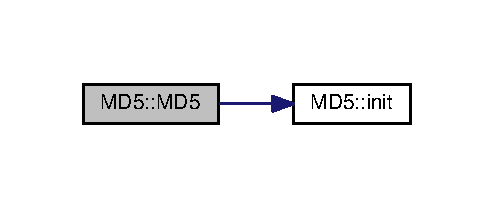
\includegraphics[width=237pt]{classMD5_afa6155ec36de415ab2dcf5e54b670d13_cgraph}
\end{center}
\end{figure}
\hypertarget{classMD5_a155356ffd713345e69e6dcbd9f8da6ce}{}\label{classMD5_a155356ffd713345e69e6dcbd9f8da6ce} 
\index{M\+D5@{M\+D5}!M\+D5@{M\+D5}}
\index{M\+D5@{M\+D5}!M\+D5@{M\+D5}}
\subsubsection{\texorpdfstring{M\+D5()}{MD5()}\hspace{0.1cm}{\footnotesize\ttfamily [2/2]}}
{\footnotesize\ttfamily M\+D5\+::\+M\+D5 (\begin{DoxyParamCaption}\item[{const std\+::string \&}]{text }\end{DoxyParamCaption})}



Definición en la línea 114 del archivo md5.\+cpp.



Hace referencia a finalize(), init() y update().

Gráfico de llamadas para esta función\+:\nopagebreak
\begin{figure}[H]
\begin{center}
\leavevmode
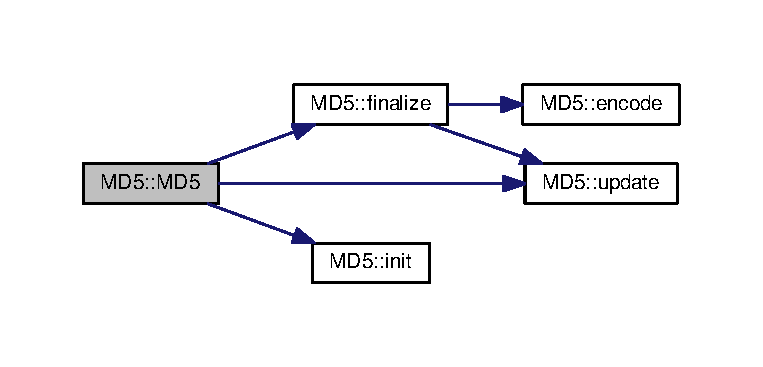
\includegraphics[width=350pt]{classMD5_a155356ffd713345e69e6dcbd9f8da6ce_cgraph}
\end{center}
\end{figure}


\subsection{Documentación de las funciones miembro}
\hypertarget{classMD5_a7eef3463c43a2cdfb56a0261b640f873}{}\label{classMD5_a7eef3463c43a2cdfb56a0261b640f873} 
\index{M\+D5@{M\+D5}!decode@{decode}}
\index{decode@{decode}!M\+D5@{M\+D5}}
\subsubsection{\texorpdfstring{decode()}{decode()}}
{\footnotesize\ttfamily void M\+D5\+::decode (\begin{DoxyParamCaption}\item[{\hyperlink{classMD5_a2e5b84a3d7db292f49873061214a0444}{uint4}}]{output\mbox{[}$\,$\mbox{]},  }\item[{const \hyperlink{classMD5_a3b1c4901139aef256ee49c4ab14d09f9}{uint1}}]{input\mbox{[}$\,$\mbox{]},  }\item[{\hyperlink{classMD5_aa836972700679dbcff6ae8337f6db464}{size\+\_\+type}}]{len }\end{DoxyParamCaption})\hspace{0.3cm}{\ttfamily [static]}, {\ttfamily [private]}}



Definición en la línea 137 del archivo md5.\+cpp.



Referenciado por transform().

\hypertarget{classMD5_a52603a1b589b2863cad4caae7f259b7e}{}\label{classMD5_a52603a1b589b2863cad4caae7f259b7e} 
\index{M\+D5@{M\+D5}!encode@{encode}}
\index{encode@{encode}!M\+D5@{M\+D5}}
\subsubsection{\texorpdfstring{encode()}{encode()}}
{\footnotesize\ttfamily void M\+D5\+::encode (\begin{DoxyParamCaption}\item[{\hyperlink{classMD5_a3b1c4901139aef256ee49c4ab14d09f9}{uint1}}]{output\mbox{[}$\,$\mbox{]},  }\item[{const \hyperlink{classMD5_a2e5b84a3d7db292f49873061214a0444}{uint4}}]{input\mbox{[}$\,$\mbox{]},  }\item[{\hyperlink{classMD5_aa836972700679dbcff6ae8337f6db464}{size\+\_\+type}}]{len }\end{DoxyParamCaption})\hspace{0.3cm}{\ttfamily [static]}, {\ttfamily [private]}}



Definición en la línea 147 del archivo md5.\+cpp.



Referenciado por finalize().

\hypertarget{classMD5_a95b7adf4602b92e84ca5f34084859e79}{}\label{classMD5_a95b7adf4602b92e84ca5f34084859e79} 
\index{M\+D5@{M\+D5}!F@{F}}
\index{F@{F}!M\+D5@{M\+D5}}
\subsubsection{\texorpdfstring{F()}{F()}}
{\footnotesize\ttfamily \hyperlink{classMD5_a2e5b84a3d7db292f49873061214a0444}{M\+D5\+::uint4} M\+D5\+::F (\begin{DoxyParamCaption}\item[{\hyperlink{classMD5_a2e5b84a3d7db292f49873061214a0444}{uint4}}]{x,  }\item[{\hyperlink{classMD5_a2e5b84a3d7db292f49873061214a0444}{uint4}}]{y,  }\item[{\hyperlink{classMD5_a2e5b84a3d7db292f49873061214a0444}{uint4}}]{z }\end{DoxyParamCaption})\hspace{0.3cm}{\ttfamily [inline]}, {\ttfamily [static]}, {\ttfamily [private]}}



Definición en la línea 66 del archivo md5.\+cpp.



Referenciado por F\+F().

\hypertarget{classMD5_a31479b157441ace2dbc2ae0edd0d2e38}{}\label{classMD5_a31479b157441ace2dbc2ae0edd0d2e38} 
\index{M\+D5@{M\+D5}!FF@{FF}}
\index{FF@{FF}!M\+D5@{M\+D5}}
\subsubsection{\texorpdfstring{F\+F()}{FF()}}
{\footnotesize\ttfamily void M\+D5\+::\+FF (\begin{DoxyParamCaption}\item[{\hyperlink{classMD5_a2e5b84a3d7db292f49873061214a0444}{uint4} \&}]{a,  }\item[{\hyperlink{classMD5_a2e5b84a3d7db292f49873061214a0444}{uint4}}]{b,  }\item[{\hyperlink{classMD5_a2e5b84a3d7db292f49873061214a0444}{uint4}}]{c,  }\item[{\hyperlink{classMD5_a2e5b84a3d7db292f49873061214a0444}{uint4}}]{d,  }\item[{\hyperlink{classMD5_a2e5b84a3d7db292f49873061214a0444}{uint4}}]{x,  }\item[{\hyperlink{classMD5_a2e5b84a3d7db292f49873061214a0444}{uint4}}]{s,  }\item[{\hyperlink{classMD5_a2e5b84a3d7db292f49873061214a0444}{uint4}}]{ac }\end{DoxyParamCaption})\hspace{0.3cm}{\ttfamily [inline]}, {\ttfamily [static]}, {\ttfamily [private]}}



Definición en la línea 89 del archivo md5.\+cpp.



Hace referencia a F() y rotate\+\_\+left().



Referenciado por transform().

Gráfico de llamadas para esta función\+:\nopagebreak
\begin{figure}[H]
\begin{center}
\leavevmode
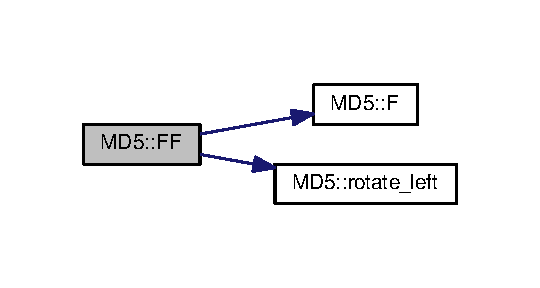
\includegraphics[width=259pt]{classMD5_a31479b157441ace2dbc2ae0edd0d2e38_cgraph}
\end{center}
\end{figure}
\hypertarget{classMD5_a10f607494a3f2e3e515fc4b99d1a06cc}{}\label{classMD5_a10f607494a3f2e3e515fc4b99d1a06cc} 
\index{M\+D5@{M\+D5}!finalize@{finalize}}
\index{finalize@{finalize}!M\+D5@{M\+D5}}
\subsubsection{\texorpdfstring{finalize()}{finalize()}}
{\footnotesize\ttfamily \hyperlink{classMD5}{M\+D5} \& M\+D5\+::finalize (\begin{DoxyParamCaption}{ }\end{DoxyParamCaption})}



Definición en la línea 292 del archivo md5.\+cpp.



Hace referencia a buffer, count, digest, encode(), finalized, state y update().



Referenciado por M\+D5().

Gráfico de llamadas para esta función\+:\nopagebreak
\begin{figure}[H]
\begin{center}
\leavevmode
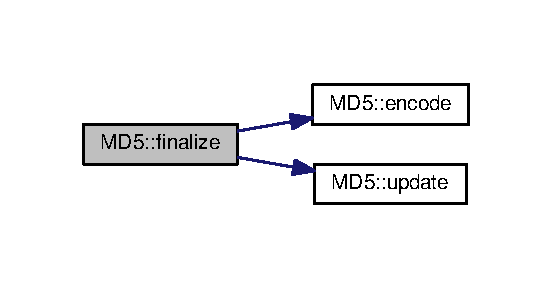
\includegraphics[width=265pt]{classMD5_a10f607494a3f2e3e515fc4b99d1a06cc_cgraph}
\end{center}
\end{figure}
\hypertarget{classMD5_afbc3ab3591fca4e780f647dac3952bc8}{}\label{classMD5_afbc3ab3591fca4e780f647dac3952bc8} 
\index{M\+D5@{M\+D5}!G@{G}}
\index{G@{G}!M\+D5@{M\+D5}}
\subsubsection{\texorpdfstring{G()}{G()}}
{\footnotesize\ttfamily \hyperlink{classMD5_a2e5b84a3d7db292f49873061214a0444}{M\+D5\+::uint4} M\+D5\+::G (\begin{DoxyParamCaption}\item[{\hyperlink{classMD5_a2e5b84a3d7db292f49873061214a0444}{uint4}}]{x,  }\item[{\hyperlink{classMD5_a2e5b84a3d7db292f49873061214a0444}{uint4}}]{y,  }\item[{\hyperlink{classMD5_a2e5b84a3d7db292f49873061214a0444}{uint4}}]{z }\end{DoxyParamCaption})\hspace{0.3cm}{\ttfamily [inline]}, {\ttfamily [static]}, {\ttfamily [private]}}



Definición en la línea 70 del archivo md5.\+cpp.



Referenciado por G\+G().

\hypertarget{classMD5_a8ebdbe52608e522516d1759a31753212}{}\label{classMD5_a8ebdbe52608e522516d1759a31753212} 
\index{M\+D5@{M\+D5}!GG@{GG}}
\index{GG@{GG}!M\+D5@{M\+D5}}
\subsubsection{\texorpdfstring{G\+G()}{GG()}}
{\footnotesize\ttfamily void M\+D5\+::\+GG (\begin{DoxyParamCaption}\item[{\hyperlink{classMD5_a2e5b84a3d7db292f49873061214a0444}{uint4} \&}]{a,  }\item[{\hyperlink{classMD5_a2e5b84a3d7db292f49873061214a0444}{uint4}}]{b,  }\item[{\hyperlink{classMD5_a2e5b84a3d7db292f49873061214a0444}{uint4}}]{c,  }\item[{\hyperlink{classMD5_a2e5b84a3d7db292f49873061214a0444}{uint4}}]{d,  }\item[{\hyperlink{classMD5_a2e5b84a3d7db292f49873061214a0444}{uint4}}]{x,  }\item[{\hyperlink{classMD5_a2e5b84a3d7db292f49873061214a0444}{uint4}}]{s,  }\item[{\hyperlink{classMD5_a2e5b84a3d7db292f49873061214a0444}{uint4}}]{ac }\end{DoxyParamCaption})\hspace{0.3cm}{\ttfamily [inline]}, {\ttfamily [static]}, {\ttfamily [private]}}



Definición en la línea 93 del archivo md5.\+cpp.



Hace referencia a G() y rotate\+\_\+left().



Referenciado por transform().

Gráfico de llamadas para esta función\+:\nopagebreak
\begin{figure}[H]
\begin{center}
\leavevmode
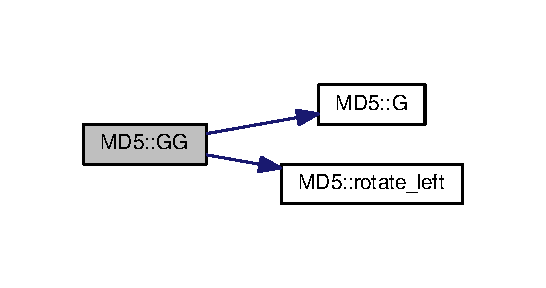
\includegraphics[width=262pt]{classMD5_a8ebdbe52608e522516d1759a31753212_cgraph}
\end{center}
\end{figure}
\hypertarget{classMD5_a59392e8552045b37628a48497ede9cf0}{}\label{classMD5_a59392e8552045b37628a48497ede9cf0} 
\index{M\+D5@{M\+D5}!H@{H}}
\index{H@{H}!M\+D5@{M\+D5}}
\subsubsection{\texorpdfstring{H()}{H()}}
{\footnotesize\ttfamily \hyperlink{classMD5_a2e5b84a3d7db292f49873061214a0444}{M\+D5\+::uint4} M\+D5\+::H (\begin{DoxyParamCaption}\item[{\hyperlink{classMD5_a2e5b84a3d7db292f49873061214a0444}{uint4}}]{x,  }\item[{\hyperlink{classMD5_a2e5b84a3d7db292f49873061214a0444}{uint4}}]{y,  }\item[{\hyperlink{classMD5_a2e5b84a3d7db292f49873061214a0444}{uint4}}]{z }\end{DoxyParamCaption})\hspace{0.3cm}{\ttfamily [inline]}, {\ttfamily [static]}, {\ttfamily [private]}}



Definición en la línea 74 del archivo md5.\+cpp.



Referenciado por H\+H().

\hypertarget{classMD5_aaf466f683b4bd8b1b66544f48bf09608}{}\label{classMD5_aaf466f683b4bd8b1b66544f48bf09608} 
\index{M\+D5@{M\+D5}!hexdigest@{hexdigest}}
\index{hexdigest@{hexdigest}!M\+D5@{M\+D5}}
\subsubsection{\texorpdfstring{hexdigest()}{hexdigest()}}
{\footnotesize\ttfamily std\+::string M\+D5\+::hexdigest (\begin{DoxyParamCaption}{ }\end{DoxyParamCaption}) const}



Definición en la línea 329 del archivo md5.\+cpp.



Hace referencia a digest y finalized.



Referenciado por md5() y operator$<$$<$().

\hypertarget{classMD5_aaad039caf0b33abf1bf3f3589166543c}{}\label{classMD5_aaad039caf0b33abf1bf3f3589166543c} 
\index{M\+D5@{M\+D5}!HH@{HH}}
\index{HH@{HH}!M\+D5@{M\+D5}}
\subsubsection{\texorpdfstring{H\+H()}{HH()}}
{\footnotesize\ttfamily void M\+D5\+::\+HH (\begin{DoxyParamCaption}\item[{\hyperlink{classMD5_a2e5b84a3d7db292f49873061214a0444}{uint4} \&}]{a,  }\item[{\hyperlink{classMD5_a2e5b84a3d7db292f49873061214a0444}{uint4}}]{b,  }\item[{\hyperlink{classMD5_a2e5b84a3d7db292f49873061214a0444}{uint4}}]{c,  }\item[{\hyperlink{classMD5_a2e5b84a3d7db292f49873061214a0444}{uint4}}]{d,  }\item[{\hyperlink{classMD5_a2e5b84a3d7db292f49873061214a0444}{uint4}}]{x,  }\item[{\hyperlink{classMD5_a2e5b84a3d7db292f49873061214a0444}{uint4}}]{s,  }\item[{\hyperlink{classMD5_a2e5b84a3d7db292f49873061214a0444}{uint4}}]{ac }\end{DoxyParamCaption})\hspace{0.3cm}{\ttfamily [inline]}, {\ttfamily [static]}, {\ttfamily [private]}}



Definición en la línea 97 del archivo md5.\+cpp.



Hace referencia a H() y rotate\+\_\+left().



Referenciado por transform().

Gráfico de llamadas para esta función\+:\nopagebreak
\begin{figure}[H]
\begin{center}
\leavevmode
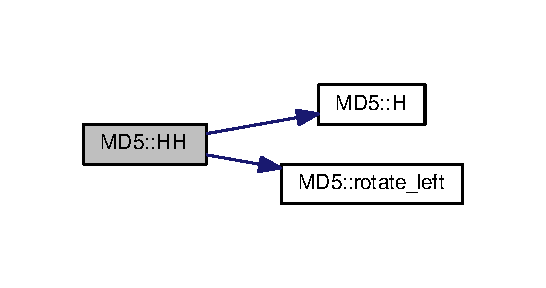
\includegraphics[width=262pt]{classMD5_aaad039caf0b33abf1bf3f3589166543c_cgraph}
\end{center}
\end{figure}
\hypertarget{classMD5_ad2c1682834e38219894728830e3996c3}{}\label{classMD5_ad2c1682834e38219894728830e3996c3} 
\index{M\+D5@{M\+D5}!I@{I}}
\index{I@{I}!M\+D5@{M\+D5}}
\subsubsection{\texorpdfstring{I()}{I()}}
{\footnotesize\ttfamily \hyperlink{classMD5_a2e5b84a3d7db292f49873061214a0444}{M\+D5\+::uint4} M\+D5\+::I (\begin{DoxyParamCaption}\item[{\hyperlink{classMD5_a2e5b84a3d7db292f49873061214a0444}{uint4}}]{x,  }\item[{\hyperlink{classMD5_a2e5b84a3d7db292f49873061214a0444}{uint4}}]{y,  }\item[{\hyperlink{classMD5_a2e5b84a3d7db292f49873061214a0444}{uint4}}]{z }\end{DoxyParamCaption})\hspace{0.3cm}{\ttfamily [inline]}, {\ttfamily [static]}, {\ttfamily [private]}}



Definición en la línea 78 del archivo md5.\+cpp.



Referenciado por I\+I().

\hypertarget{classMD5_a7af0184654644964ecdb57b1203e5ec7}{}\label{classMD5_a7af0184654644964ecdb57b1203e5ec7} 
\index{M\+D5@{M\+D5}!II@{II}}
\index{II@{II}!M\+D5@{M\+D5}}
\subsubsection{\texorpdfstring{I\+I()}{II()}}
{\footnotesize\ttfamily void M\+D5\+::\+II (\begin{DoxyParamCaption}\item[{\hyperlink{classMD5_a2e5b84a3d7db292f49873061214a0444}{uint4} \&}]{a,  }\item[{\hyperlink{classMD5_a2e5b84a3d7db292f49873061214a0444}{uint4}}]{b,  }\item[{\hyperlink{classMD5_a2e5b84a3d7db292f49873061214a0444}{uint4}}]{c,  }\item[{\hyperlink{classMD5_a2e5b84a3d7db292f49873061214a0444}{uint4}}]{d,  }\item[{\hyperlink{classMD5_a2e5b84a3d7db292f49873061214a0444}{uint4}}]{x,  }\item[{\hyperlink{classMD5_a2e5b84a3d7db292f49873061214a0444}{uint4}}]{s,  }\item[{\hyperlink{classMD5_a2e5b84a3d7db292f49873061214a0444}{uint4}}]{ac }\end{DoxyParamCaption})\hspace{0.3cm}{\ttfamily [inline]}, {\ttfamily [static]}, {\ttfamily [private]}}



Definición en la línea 101 del archivo md5.\+cpp.



Hace referencia a I() y rotate\+\_\+left().



Referenciado por transform().

Gráfico de llamadas para esta función\+:\nopagebreak
\begin{figure}[H]
\begin{center}
\leavevmode
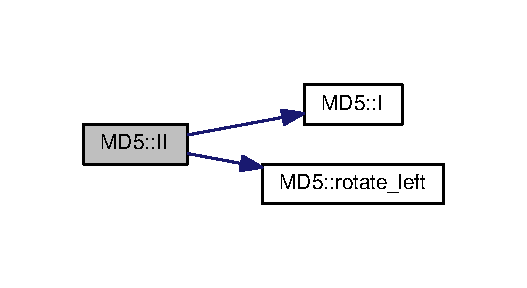
\includegraphics[width=253pt]{classMD5_a7af0184654644964ecdb57b1203e5ec7_cgraph}
\end{center}
\end{figure}
\hypertarget{classMD5_a65ddaecdd0bd0b09043a2f3b2601bc2e}{}\label{classMD5_a65ddaecdd0bd0b09043a2f3b2601bc2e} 
\index{M\+D5@{M\+D5}!init@{init}}
\index{init@{init}!M\+D5@{M\+D5}}
\subsubsection{\texorpdfstring{init()}{init()}}
{\footnotesize\ttfamily void M\+D5\+::init (\begin{DoxyParamCaption}{ }\end{DoxyParamCaption})\hspace{0.3cm}{\ttfamily [private]}}



Definición en la línea 121 del archivo md5.\+cpp.



Hace referencia a count, finalized y state.



Referenciado por M\+D5().

\hypertarget{classMD5_a97ece3d8221e3c9c994aa9d13001b1d9}{}\label{classMD5_a97ece3d8221e3c9c994aa9d13001b1d9} 
\index{M\+D5@{M\+D5}!rotate\+\_\+left@{rotate\+\_\+left}}
\index{rotate\+\_\+left@{rotate\+\_\+left}!M\+D5@{M\+D5}}
\subsubsection{\texorpdfstring{rotate\+\_\+left()}{rotate\_left()}}
{\footnotesize\ttfamily \hyperlink{classMD5_a2e5b84a3d7db292f49873061214a0444}{M\+D5\+::uint4} M\+D5\+::rotate\+\_\+left (\begin{DoxyParamCaption}\item[{\hyperlink{classMD5_a2e5b84a3d7db292f49873061214a0444}{uint4}}]{x,  }\item[{int}]{n }\end{DoxyParamCaption})\hspace{0.3cm}{\ttfamily [inline]}, {\ttfamily [static]}, {\ttfamily [private]}}



Definición en la línea 83 del archivo md5.\+cpp.



Referenciado por F\+F(), G\+G(), H\+H() y I\+I().

\hypertarget{classMD5_a9d569ab2a3e564793e116f774a3ad269}{}\label{classMD5_a9d569ab2a3e564793e116f774a3ad269} 
\index{M\+D5@{M\+D5}!transform@{transform}}
\index{transform@{transform}!M\+D5@{M\+D5}}
\subsubsection{\texorpdfstring{transform()}{transform()}}
{\footnotesize\ttfamily void M\+D5\+::transform (\begin{DoxyParamCaption}\item[{const \hyperlink{classMD5_a3b1c4901139aef256ee49c4ab14d09f9}{uint1}}]{block\mbox{[}blocksize\mbox{]} }\end{DoxyParamCaption})\hspace{0.3cm}{\ttfamily [private]}}



Definición en la línea 159 del archivo md5.\+cpp.



Hace referencia a blocksize, buffer, count, decode(), F\+F(), G\+G(), H\+H(), I\+I(), S11, S12, S13, S14, S21, S22, S23, S24, S31, S32, S33, S34, S41, S42, S43, S44, state y update().

Gráfico de llamadas para esta función\+:\nopagebreak
\begin{figure}[H]
\begin{center}
\leavevmode
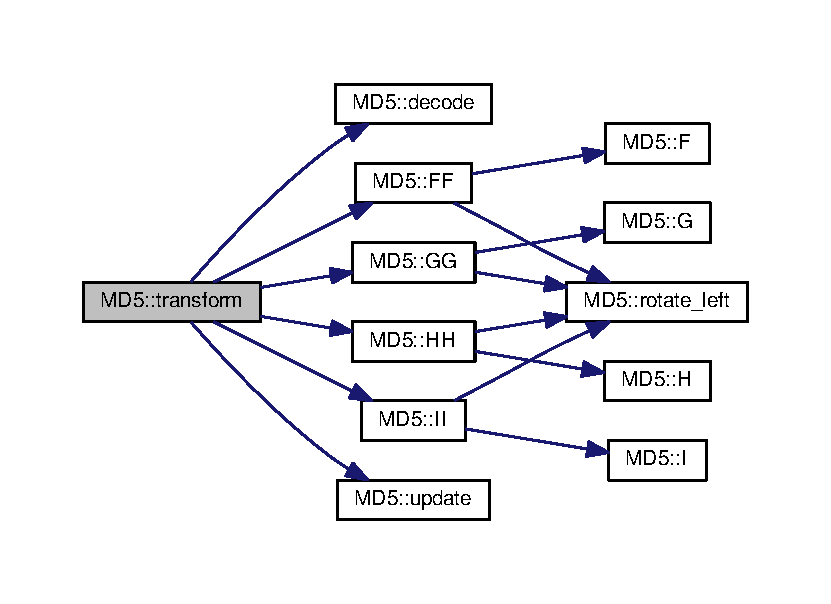
\includegraphics[width=350pt]{classMD5_a9d569ab2a3e564793e116f774a3ad269_cgraph}
\end{center}
\end{figure}
\hypertarget{classMD5_ac5ddf6cd8f940422396d321ea90ed045}{}\label{classMD5_ac5ddf6cd8f940422396d321ea90ed045} 
\index{M\+D5@{M\+D5}!update@{update}}
\index{update@{update}!M\+D5@{M\+D5}}
\subsubsection{\texorpdfstring{update()}{update()}\hspace{0.1cm}{\footnotesize\ttfamily [1/2]}}
{\footnotesize\ttfamily void M\+D5\+::update (\begin{DoxyParamCaption}\item[{const unsigned char $\ast$}]{buf,  }\item[{\hyperlink{classMD5_aa836972700679dbcff6ae8337f6db464}{size\+\_\+type}}]{length }\end{DoxyParamCaption})}



Referenciado por finalize(), M\+D5() y transform().

\hypertarget{classMD5_ac5ccba375539b993958fb235f8ac849c}{}\label{classMD5_ac5ccba375539b993958fb235f8ac849c} 
\index{M\+D5@{M\+D5}!update@{update}}
\index{update@{update}!M\+D5@{M\+D5}}
\subsubsection{\texorpdfstring{update()}{update()}\hspace{0.1cm}{\footnotesize\ttfamily [2/2]}}
{\footnotesize\ttfamily void M\+D5\+::update (\begin{DoxyParamCaption}\item[{const char $\ast$}]{buf,  }\item[{\hyperlink{classMD5_aa836972700679dbcff6ae8337f6db464}{size\+\_\+type}}]{length }\end{DoxyParamCaption})}



\subsection{Documentación de las funciones relacionadas y clases amigas}
\hypertarget{classMD5_a0739666fd0f3a7117546f6c50e0783b2}{}\label{classMD5_a0739666fd0f3a7117546f6c50e0783b2} 
\index{M\+D5@{M\+D5}!operator$<$$<$@{operator$<$$<$}}
\index{operator$<$$<$@{operator$<$$<$}!M\+D5@{M\+D5}}
\subsubsection{\texorpdfstring{operator$<$$<$}{operator<<}}
{\footnotesize\ttfamily std\+::ostream\& operator$<$$<$ (\begin{DoxyParamCaption}\item[{std\+::ostream \&}]{out,  }\item[{\hyperlink{classMD5}{M\+D5}}]{md5 }\end{DoxyParamCaption})\hspace{0.3cm}{\ttfamily [friend]}}



Definición en la línea 344 del archivo md5.\+cpp.



\subsection{Documentación de los datos miembro}
\hypertarget{classMD5_a0df603b8332399d5c1daa08ab5a315ea}{}\label{classMD5_a0df603b8332399d5c1daa08ab5a315ea} 
\index{M\+D5@{M\+D5}!buffer@{buffer}}
\index{buffer@{buffer}!M\+D5@{M\+D5}}
\subsubsection{\texorpdfstring{buffer}{buffer}}
{\footnotesize\ttfamily \hyperlink{classMD5_a3b1c4901139aef256ee49c4ab14d09f9}{uint1} M\+D5\+::buffer\mbox{[}\hyperlink{classMD5_a227e6f16f2409956b516b453e6bc7429a1cc0a742ca803f75a021aef77b522963}{blocksize}\mbox{]}\hspace{0.3cm}{\ttfamily [private]}}



Definición en la línea 94 del archivo md5.\+h.



Referenciado por finalize() y transform().

\hypertarget{classMD5_a52a9ff26a3de9e831b17c1740aa5388a}{}\label{classMD5_a52a9ff26a3de9e831b17c1740aa5388a} 
\index{M\+D5@{M\+D5}!count@{count}}
\index{count@{count}!M\+D5@{M\+D5}}
\subsubsection{\texorpdfstring{count}{count}}
{\footnotesize\ttfamily \hyperlink{classMD5_a2e5b84a3d7db292f49873061214a0444}{uint4} M\+D5\+::count\mbox{[}2\mbox{]}\hspace{0.3cm}{\ttfamily [private]}}



Definición en la línea 95 del archivo md5.\+h.



Referenciado por finalize(), init() y transform().

\hypertarget{classMD5_a31058e1dca10bbf29818bb5177ff02ac}{}\label{classMD5_a31058e1dca10bbf29818bb5177ff02ac} 
\index{M\+D5@{M\+D5}!digest@{digest}}
\index{digest@{digest}!M\+D5@{M\+D5}}
\subsubsection{\texorpdfstring{digest}{digest}}
{\footnotesize\ttfamily \hyperlink{classMD5_a3b1c4901139aef256ee49c4ab14d09f9}{uint1} M\+D5\+::digest\mbox{[}16\mbox{]}\hspace{0.3cm}{\ttfamily [private]}}



Definición en la línea 97 del archivo md5.\+h.



Referenciado por finalize() y hexdigest().

\hypertarget{classMD5_a696e995f7045cf0146a207c720386f9c}{}\label{classMD5_a696e995f7045cf0146a207c720386f9c} 
\index{M\+D5@{M\+D5}!finalized@{finalized}}
\index{finalized@{finalized}!M\+D5@{M\+D5}}
\subsubsection{\texorpdfstring{finalized}{finalized}}
{\footnotesize\ttfamily bool M\+D5\+::finalized\hspace{0.3cm}{\ttfamily [private]}}



Definición en la línea 93 del archivo md5.\+h.



Referenciado por finalize(), hexdigest() y init().

\hypertarget{classMD5_aae3f861952f5b129463f550170836db0}{}\label{classMD5_aae3f861952f5b129463f550170836db0} 
\index{M\+D5@{M\+D5}!state@{state}}
\index{state@{state}!M\+D5@{M\+D5}}
\subsubsection{\texorpdfstring{state}{state}}
{\footnotesize\ttfamily \hyperlink{classMD5_a2e5b84a3d7db292f49873061214a0444}{uint4} M\+D5\+::state\mbox{[}4\mbox{]}\hspace{0.3cm}{\ttfamily [private]}}



Definición en la línea 96 del archivo md5.\+h.



Referenciado por finalize(), init() y transform().



La documentación para esta clase fue generada a partir de los siguientes ficheros\+:\begin{DoxyCompactItemize}
\item 
Template\+A\+F\+I\+S\+\_\+webservice\+\_\+lib/firma\+\_\+digital/\hyperlink{md5_8h}{md5.\+h}\item 
Template\+A\+F\+I\+S\+\_\+webservice\+\_\+lib/firma\+\_\+digital/\hyperlink{md5_8cpp}{md5.\+cpp}\end{DoxyCompactItemize}

\hypertarget{classSHA512}{}\section{Referencia de la Clase S\+H\+A512}
\label{classSHA512}\index{S\+H\+A512@{S\+H\+A512}}


Clase de la comunidad\+: Se incluyó para estabilizar \hyperlink{md5_8cpp}{md5.\+cpp} para evitar que, si el cliente tiene una versión diferente de las bibliotecas de \hyperlink{classMD5}{M\+D5} o de \hyperlink{classSHA512}{S\+H\+A512} que el servidor, no choquen.  




{\ttfamily \#include $<$sha512.\+h$>$}

\subsection*{Métodos públicos}
\begin{DoxyCompactItemize}
\item 
void \hyperlink{classSHA512_a92d7e88a28d0bd70930df68bfcd4d136}{init} ()
\item 
void \hyperlink{classSHA512_aa1c4c23e601cbc51deda2fecbfed71d6}{update} (const unsigned char $\ast$message, unsigned int len)
\item 
void \hyperlink{classSHA512_a6db56be0379bbf38babee9567356ad68}{final} (unsigned char $\ast$digest)
\end{DoxyCompactItemize}
\subsection*{Atributos públicos estáticos}
\begin{DoxyCompactItemize}
\item 
static const unsigned int \hyperlink{classSHA512_a911d66aedbff405df349ef300791d8eb}{D\+I\+G\+E\+S\+T\+\_\+\+S\+I\+ZE} = ( 512 / 8)
\end{DoxyCompactItemize}
\subsection*{Tipos protegidos}
\begin{DoxyCompactItemize}
\item 
typedef unsigned char \hyperlink{classSHA512_a92a2b23b4b5217fefcb5b1884f40c054}{uint8}
\item 
typedef unsigned long \hyperlink{classSHA512_a52085ac598de8ad6c5f157eafcefc047}{uint32}
\item 
typedef unsigned long long \hyperlink{classSHA512_af8e6d233ae15030174e481d6d79b1786}{uint64}
\end{DoxyCompactItemize}
\subsection*{Métodos protegidos}
\begin{DoxyCompactItemize}
\item 
void \hyperlink{classSHA512_aaa6717d3ffe1b8efa2d17b838276ab29}{transform} (const unsigned char $\ast$message, unsigned int block\+\_\+nb)
\end{DoxyCompactItemize}
\subsection*{Atributos protegidos}
\begin{DoxyCompactItemize}
\item 
unsigned int \hyperlink{classSHA512_a99134ffe06076eaf88e6db543304d0ef}{m\+\_\+tot\+\_\+len}
\item 
unsigned int \hyperlink{classSHA512_ac08a6cd41b96a9ca98ca567c3225bdca}{m\+\_\+len}
\item 
unsigned char \hyperlink{classSHA512_aef099f8df4da2e3ea0a56bf5f0479fce}{m\+\_\+block} \mbox{[}2 $\ast$\hyperlink{classSHA512_a5191f35aa313f5fd0447d2c272a82c99}{S\+H\+A384\+\_\+512\+\_\+\+B\+L\+O\+C\+K\+\_\+\+S\+I\+ZE}\mbox{]}
\item 
\hyperlink{classSHA512_af8e6d233ae15030174e481d6d79b1786}{uint64} \hyperlink{classSHA512_a6fcfcd454382329628cd6baa0487bee5}{m\+\_\+h} \mbox{[}8\mbox{]}
\end{DoxyCompactItemize}
\subsection*{Atributos protegidos estáticos}
\begin{DoxyCompactItemize}
\item 
static const \hyperlink{classSHA512_af8e6d233ae15030174e481d6d79b1786}{uint64} \hyperlink{classSHA512_af6d393ef5aa7458c3545efa1b9d92900}{sha512\+\_\+k} \mbox{[}$\,$\mbox{]}
\item 
static const unsigned int \hyperlink{classSHA512_a5191f35aa313f5fd0447d2c272a82c99}{S\+H\+A384\+\_\+512\+\_\+\+B\+L\+O\+C\+K\+\_\+\+S\+I\+ZE} = (1024/8)
\end{DoxyCompactItemize}


\subsection{Descripción detallada}
Clase de la comunidad\+: Se incluyó para estabilizar \hyperlink{md5_8cpp}{md5.\+cpp} para evitar que, si el cliente tiene una versión diferente de las bibliotecas de \hyperlink{classMD5}{M\+D5} o de \hyperlink{classSHA512}{S\+H\+A512} que el servidor, no choquen. 

Definición en la línea 60 del archivo sha512.\+h.



\subsection{Documentación de los \textquotesingle{}Typedef\textquotesingle{} miembros de la clase}
\hypertarget{classSHA512_a52085ac598de8ad6c5f157eafcefc047}{}\label{classSHA512_a52085ac598de8ad6c5f157eafcefc047} 
\index{S\+H\+A512@{S\+H\+A512}!uint32@{uint32}}
\index{uint32@{uint32}!S\+H\+A512@{S\+H\+A512}}
\subsubsection{\texorpdfstring{uint32}{uint32}}
{\footnotesize\ttfamily typedef unsigned long \hyperlink{classSHA512_a52085ac598de8ad6c5f157eafcefc047}{S\+H\+A512\+::uint32}\hspace{0.3cm}{\ttfamily [protected]}}



Definición en la línea 64 del archivo sha512.\+h.

\hypertarget{classSHA512_af8e6d233ae15030174e481d6d79b1786}{}\label{classSHA512_af8e6d233ae15030174e481d6d79b1786} 
\index{S\+H\+A512@{S\+H\+A512}!uint64@{uint64}}
\index{uint64@{uint64}!S\+H\+A512@{S\+H\+A512}}
\subsubsection{\texorpdfstring{uint64}{uint64}}
{\footnotesize\ttfamily typedef unsigned long long \hyperlink{classSHA512_af8e6d233ae15030174e481d6d79b1786}{S\+H\+A512\+::uint64}\hspace{0.3cm}{\ttfamily [protected]}}



Definición en la línea 65 del archivo sha512.\+h.

\hypertarget{classSHA512_a92a2b23b4b5217fefcb5b1884f40c054}{}\label{classSHA512_a92a2b23b4b5217fefcb5b1884f40c054} 
\index{S\+H\+A512@{S\+H\+A512}!uint8@{uint8}}
\index{uint8@{uint8}!S\+H\+A512@{S\+H\+A512}}
\subsubsection{\texorpdfstring{uint8}{uint8}}
{\footnotesize\ttfamily typedef unsigned char \hyperlink{classSHA512_a92a2b23b4b5217fefcb5b1884f40c054}{S\+H\+A512\+::uint8}\hspace{0.3cm}{\ttfamily [protected]}}



Definición en la línea 63 del archivo sha512.\+h.



\subsection{Documentación de las funciones miembro}
\hypertarget{classSHA512_a6db56be0379bbf38babee9567356ad68}{}\label{classSHA512_a6db56be0379bbf38babee9567356ad68} 
\index{S\+H\+A512@{S\+H\+A512}!final@{final}}
\index{final@{final}!S\+H\+A512@{S\+H\+A512}}
\subsubsection{\texorpdfstring{final()}{final()}}
{\footnotesize\ttfamily void S\+H\+A512\+::final (\begin{DoxyParamCaption}\item[{unsigned char $\ast$}]{digest }\end{DoxyParamCaption})}



Definición en la línea 130 del archivo sha512.\+cpp.



Hace referencia a m\+\_\+block, m\+\_\+h, m\+\_\+len, m\+\_\+tot\+\_\+len, S\+H\+A2\+\_\+\+U\+N\+P\+A\+C\+K32, S\+H\+A2\+\_\+\+U\+N\+P\+A\+C\+K64, S\+H\+A384\+\_\+512\+\_\+\+B\+L\+O\+C\+K\+\_\+\+S\+I\+ZE y transform().



Referenciado por sha512().

Gráfico de llamadas para esta función\+:\nopagebreak
\begin{figure}[H]
\begin{center}
\leavevmode
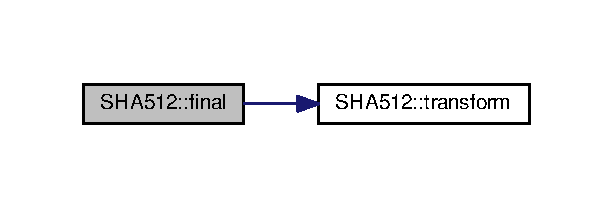
\includegraphics[width=294pt]{classSHA512_a6db56be0379bbf38babee9567356ad68_cgraph}
\end{center}
\end{figure}
\hypertarget{classSHA512_a92d7e88a28d0bd70930df68bfcd4d136}{}\label{classSHA512_a92d7e88a28d0bd70930df68bfcd4d136} 
\index{S\+H\+A512@{S\+H\+A512}!init@{init}}
\index{init@{init}!S\+H\+A512@{S\+H\+A512}}
\subsubsection{\texorpdfstring{init()}{init()}}
{\footnotesize\ttfamily void S\+H\+A512\+::init (\begin{DoxyParamCaption}{ }\end{DoxyParamCaption})}



Definición en la línea 93 del archivo sha512.\+cpp.



Hace referencia a m\+\_\+h, m\+\_\+len y m\+\_\+tot\+\_\+len.



Referenciado por sha512().

\hypertarget{classSHA512_aaa6717d3ffe1b8efa2d17b838276ab29}{}\label{classSHA512_aaa6717d3ffe1b8efa2d17b838276ab29} 
\index{S\+H\+A512@{S\+H\+A512}!transform@{transform}}
\index{transform@{transform}!S\+H\+A512@{S\+H\+A512}}
\subsubsection{\texorpdfstring{transform()}{transform()}}
{\footnotesize\ttfamily void S\+H\+A512\+::transform (\begin{DoxyParamCaption}\item[{const unsigned char $\ast$}]{message,  }\item[{unsigned int}]{block\+\_\+nb }\end{DoxyParamCaption})\hspace{0.3cm}{\ttfamily [protected]}}



Definición en la línea 55 del archivo sha512.\+cpp.



Hace referencia a m\+\_\+h, S\+H\+A2\+\_\+\+CH, S\+H\+A2\+\_\+\+M\+AJ, S\+H\+A2\+\_\+\+P\+A\+C\+K64, S\+H\+A512\+\_\+\+F1, S\+H\+A512\+\_\+\+F2, S\+H\+A512\+\_\+\+F3, S\+H\+A512\+\_\+\+F4 y sha512\+\_\+k.



Referenciado por final() y update().

\hypertarget{classSHA512_aa1c4c23e601cbc51deda2fecbfed71d6}{}\label{classSHA512_aa1c4c23e601cbc51deda2fecbfed71d6} 
\index{S\+H\+A512@{S\+H\+A512}!update@{update}}
\index{update@{update}!S\+H\+A512@{S\+H\+A512}}
\subsubsection{\texorpdfstring{update()}{update()}}
{\footnotesize\ttfamily void S\+H\+A512\+::update (\begin{DoxyParamCaption}\item[{const unsigned char $\ast$}]{message,  }\item[{unsigned int}]{len }\end{DoxyParamCaption})}



Definición en la línea 107 del archivo sha512.\+cpp.



Hace referencia a m\+\_\+block, m\+\_\+len, m\+\_\+tot\+\_\+len, S\+H\+A384\+\_\+512\+\_\+\+B\+L\+O\+C\+K\+\_\+\+S\+I\+ZE y transform().



Referenciado por sha512().

Gráfico de llamadas para esta función\+:\nopagebreak
\begin{figure}[H]
\begin{center}
\leavevmode
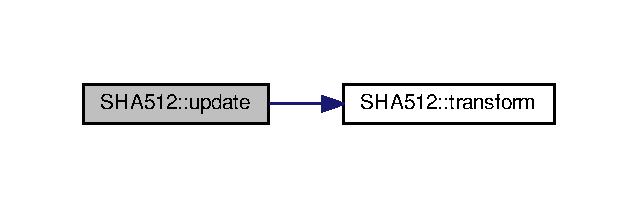
\includegraphics[width=306pt]{classSHA512_aa1c4c23e601cbc51deda2fecbfed71d6_cgraph}
\end{center}
\end{figure}


\subsection{Documentación de los datos miembro}
\hypertarget{classSHA512_a911d66aedbff405df349ef300791d8eb}{}\label{classSHA512_a911d66aedbff405df349ef300791d8eb} 
\index{S\+H\+A512@{S\+H\+A512}!D\+I\+G\+E\+S\+T\+\_\+\+S\+I\+ZE@{D\+I\+G\+E\+S\+T\+\_\+\+S\+I\+ZE}}
\index{D\+I\+G\+E\+S\+T\+\_\+\+S\+I\+ZE@{D\+I\+G\+E\+S\+T\+\_\+\+S\+I\+ZE}!S\+H\+A512@{S\+H\+A512}}
\subsubsection{\texorpdfstring{D\+I\+G\+E\+S\+T\+\_\+\+S\+I\+ZE}{DIGEST\_SIZE}}
{\footnotesize\ttfamily const unsigned int S\+H\+A512\+::\+D\+I\+G\+E\+S\+T\+\_\+\+S\+I\+ZE = ( 512 / 8)\hspace{0.3cm}{\ttfamily [static]}}



Definición en la línea 74 del archivo sha512.\+h.



Referenciado por sha512().

\hypertarget{classSHA512_aef099f8df4da2e3ea0a56bf5f0479fce}{}\label{classSHA512_aef099f8df4da2e3ea0a56bf5f0479fce} 
\index{S\+H\+A512@{S\+H\+A512}!m\+\_\+block@{m\+\_\+block}}
\index{m\+\_\+block@{m\+\_\+block}!S\+H\+A512@{S\+H\+A512}}
\subsubsection{\texorpdfstring{m\+\_\+block}{m\_block}}
{\footnotesize\ttfamily unsigned char S\+H\+A512\+::m\+\_\+block\mbox{[}2 $\ast$\hyperlink{classSHA512_a5191f35aa313f5fd0447d2c272a82c99}{S\+H\+A384\+\_\+512\+\_\+\+B\+L\+O\+C\+K\+\_\+\+S\+I\+ZE}\mbox{]}\hspace{0.3cm}{\ttfamily [protected]}}



Definición en la línea 80 del archivo sha512.\+h.



Referenciado por final() y update().

\hypertarget{classSHA512_a6fcfcd454382329628cd6baa0487bee5}{}\label{classSHA512_a6fcfcd454382329628cd6baa0487bee5} 
\index{S\+H\+A512@{S\+H\+A512}!m\+\_\+h@{m\+\_\+h}}
\index{m\+\_\+h@{m\+\_\+h}!S\+H\+A512@{S\+H\+A512}}
\subsubsection{\texorpdfstring{m\+\_\+h}{m\_h}}
{\footnotesize\ttfamily \hyperlink{classSHA512_af8e6d233ae15030174e481d6d79b1786}{uint64} S\+H\+A512\+::m\+\_\+h\mbox{[}8\mbox{]}\hspace{0.3cm}{\ttfamily [protected]}}



Definición en la línea 81 del archivo sha512.\+h.



Referenciado por final(), init() y transform().

\hypertarget{classSHA512_ac08a6cd41b96a9ca98ca567c3225bdca}{}\label{classSHA512_ac08a6cd41b96a9ca98ca567c3225bdca} 
\index{S\+H\+A512@{S\+H\+A512}!m\+\_\+len@{m\+\_\+len}}
\index{m\+\_\+len@{m\+\_\+len}!S\+H\+A512@{S\+H\+A512}}
\subsubsection{\texorpdfstring{m\+\_\+len}{m\_len}}
{\footnotesize\ttfamily unsigned int S\+H\+A512\+::m\+\_\+len\hspace{0.3cm}{\ttfamily [protected]}}



Definición en la línea 79 del archivo sha512.\+h.



Referenciado por final(), init() y update().

\hypertarget{classSHA512_a99134ffe06076eaf88e6db543304d0ef}{}\label{classSHA512_a99134ffe06076eaf88e6db543304d0ef} 
\index{S\+H\+A512@{S\+H\+A512}!m\+\_\+tot\+\_\+len@{m\+\_\+tot\+\_\+len}}
\index{m\+\_\+tot\+\_\+len@{m\+\_\+tot\+\_\+len}!S\+H\+A512@{S\+H\+A512}}
\subsubsection{\texorpdfstring{m\+\_\+tot\+\_\+len}{m\_tot\_len}}
{\footnotesize\ttfamily unsigned int S\+H\+A512\+::m\+\_\+tot\+\_\+len\hspace{0.3cm}{\ttfamily [protected]}}



Definición en la línea 78 del archivo sha512.\+h.



Referenciado por final(), init() y update().

\hypertarget{classSHA512_a5191f35aa313f5fd0447d2c272a82c99}{}\label{classSHA512_a5191f35aa313f5fd0447d2c272a82c99} 
\index{S\+H\+A512@{S\+H\+A512}!S\+H\+A384\+\_\+512\+\_\+\+B\+L\+O\+C\+K\+\_\+\+S\+I\+ZE@{S\+H\+A384\+\_\+512\+\_\+\+B\+L\+O\+C\+K\+\_\+\+S\+I\+ZE}}
\index{S\+H\+A384\+\_\+512\+\_\+\+B\+L\+O\+C\+K\+\_\+\+S\+I\+ZE@{S\+H\+A384\+\_\+512\+\_\+\+B\+L\+O\+C\+K\+\_\+\+S\+I\+ZE}!S\+H\+A512@{S\+H\+A512}}
\subsubsection{\texorpdfstring{S\+H\+A384\+\_\+512\+\_\+\+B\+L\+O\+C\+K\+\_\+\+S\+I\+ZE}{SHA384\_512\_BLOCK\_SIZE}}
{\footnotesize\ttfamily const unsigned int S\+H\+A512\+::\+S\+H\+A384\+\_\+512\+\_\+\+B\+L\+O\+C\+K\+\_\+\+S\+I\+ZE = (1024/8)\hspace{0.3cm}{\ttfamily [static]}, {\ttfamily [protected]}}



Definición en la línea 68 del archivo sha512.\+h.



Referenciado por final() y update().

\hypertarget{classSHA512_af6d393ef5aa7458c3545efa1b9d92900}{}\label{classSHA512_af6d393ef5aa7458c3545efa1b9d92900} 
\index{S\+H\+A512@{S\+H\+A512}!sha512\+\_\+k@{sha512\+\_\+k}}
\index{sha512\+\_\+k@{sha512\+\_\+k}!S\+H\+A512@{S\+H\+A512}}
\subsubsection{\texorpdfstring{sha512\+\_\+k}{sha512\_k}}
{\footnotesize\ttfamily const unsigned long long S\+H\+A512\+::sha512\+\_\+k\hspace{0.3cm}{\ttfamily [static]}, {\ttfamily [protected]}}



Definición en la línea 67 del archivo sha512.\+h.



Referenciado por transform().



La documentación para esta clase fue generada a partir de los siguientes ficheros\+:\begin{DoxyCompactItemize}
\item 
Template\+A\+F\+I\+S\+\_\+webservice\+\_\+lib/firma\+\_\+digital/\hyperlink{sha512_8h}{sha512.\+h}\item 
Template\+A\+F\+I\+S\+\_\+webservice\+\_\+lib/firma\+\_\+digital/\hyperlink{sha512_8cpp}{sha512.\+cpp}\end{DoxyCompactItemize}

\hypertarget{classTemplateAFIS__webservice}{}\section{Referencia de la Clase Template\+A\+F\+I\+S\+\_\+webservice}
\label{classTemplateAFIS__webservice}\index{Template\+A\+F\+I\+S\+\_\+webservice@{Template\+A\+F\+I\+S\+\_\+webservice}}


{\ttfamily \#include $<$Template\+A\+F\+I\+S.\+h$>$}



Diagrama de colaboración para Template\+A\+F\+I\+S\+\_\+webservice\+:\nopagebreak
\begin{figure}[H]
\begin{center}
\leavevmode
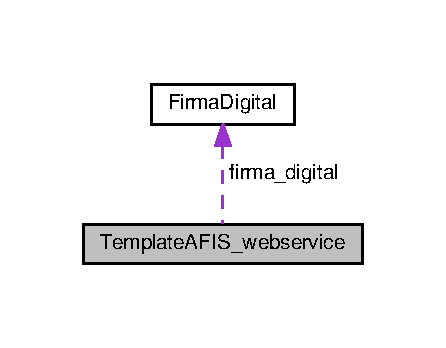
\includegraphics[width=214pt]{classTemplateAFIS__webservice__coll__graph}
\end{center}
\end{figure}
\subsection*{Métodos públicos}
\begin{DoxyCompactItemize}
\item 
\hyperlink{classTemplateAFIS__webservice_ace8ba45d6e489c7d34bfbfb55970724f}{Template\+A\+F\+I\+S\+\_\+webservice} (string param1, string param2, string param3, string param4, string param5)
\begin{DoxyCompactList}\small\item\em Constructor. \end{DoxyCompactList}\item 
\hyperlink{classTemplateAFIS__webservice_ad58b565c76e20bdd9272401d7319cb25}{$\sim$\+Template\+A\+F\+I\+S\+\_\+webservice} ()
\begin{DoxyCompactList}\small\item\em Destructor. \end{DoxyCompactList}\item 
void $\ast$ \hyperlink{classTemplateAFIS__webservice_a85f73ddfc479ea1f9ba3a6467d1c028b}{p\+El\+Mismo} ()
\begin{DoxyCompactList}\small\item\em p\+El\+Mismo \end{DoxyCompactList}\item 
void \hyperlink{classTemplateAFIS__webservice_a6357de3d3323010cb5890d2f583e0f94}{Set\+Tipo\+Template} (int tipo)
\begin{DoxyCompactList}\small\item\em Set Tipo Template. \end{DoxyCompactList}\item 
void \hyperlink{classTemplateAFIS__webservice_afc08ffa4abcde0b3c0f1c13d973755e1}{Save\+Template2\+I\+SO} ()
\begin{DoxyCompactList}\small\item\em Save Template2\+I\+SO\+: Salva el Template a I\+SO. (En pruebas) \end{DoxyCompactList}\item 
void \hyperlink{classTemplateAFIS__webservice_ae233b5bd61f6754d877e54788332fe92}{Save\+Imagen\+W\+SQ} ()
\begin{DoxyCompactList}\small\item\em Save Imagen\+W\+SQ\+: Salva el Template a W\+SQ. (En pruebas) \end{DoxyCompactList}\item 
int \hyperlink{classTemplateAFIS__webservice_a664f93880a7054b22a2b1faaacda95c3}{Get\+Security\+Level} ()
\begin{DoxyCompactList}\small\item\em Get Security Level. \end{DoxyCompactList}\item 
int \hyperlink{classTemplateAFIS__webservice_a4842d911ed73f5c33bf5150a6e3bcad4}{Get\+Fast\+Mode} ()
\begin{DoxyCompactList}\small\item\em Get Fast Mode. \end{DoxyCompactList}\item 
void \hyperlink{classTemplateAFIS__webservice_ac6ac32ddd0df850b0e25aa0943c39113}{Get\+Matcher\+Settings} ()
\begin{DoxyCompactList}\small\item\em Get Matcher Settings\+: Muestra la configuración del Matcher (Pruebas) \end{DoxyCompactList}\item 
bool \hyperlink{classTemplateAFIS__webservice_a8698c0f638f3be26a0664edd56038847}{init\+Matcher} ()
\begin{DoxyCompactList}\small\item\em Init Matcher. \end{DoxyCompactList}\item 
bool \hyperlink{classTemplateAFIS__webservice_a90522f2c2f10ae8fa3ab6abd0273b714}{un\+Init\+Matcher} ()
\begin{DoxyCompactList}\small\item\em un\+Init Matcher \end{DoxyCompactList}\item 
void \hyperlink{classTemplateAFIS__webservice_a40bd372e1a5b01d9bc2b4e1898be967f}{On\+Get\+Parameters} ()
\begin{DoxyCompactList}\small\item\em On Get Parameters. \end{DoxyCompactList}\item 
int \hyperlink{classTemplateAFIS__webservice_aa89af892ebe892d1a92f1e2dad5e998d}{On\+Set\+Template\+Type} (int value)
\begin{DoxyCompactList}\small\item\em On Set Template Type. \end{DoxyCompactList}\item 
int \hyperlink{classTemplateAFIS__webservice_a5fc2884ea75075e40a6056440021f27d}{On\+Enroll} (string usuario, string password, string id\+\_\+persona, string id\+\_\+dedo, string mano, string hash, unsigned char $\ast$\&m\+\_\+template, int m\+\_\+template\+\_\+size, unsigned char $\ast$\&p\+Image\+Data, int n\+Width, int n\+Height, string \&id\+\_\+persona\+\_\+out, string \&id\+\_\+dedo\+\_\+out, string \&mano\+\_\+out)
\begin{DoxyCompactList}\small\item\em On Enroll. \end{DoxyCompactList}\item 
int \hyperlink{classTemplateAFIS__webservice_ad2d94adf36b56bf3306e52e5e20ecaab}{On\+Verify} (string usuario, string password, string id\+\_\+proyecto, string id\+\_\+persona, string id\+\_\+dedo, string mano, unsigned char $\ast$\&Template, int Template\+Size, string \&cedula, string \&dedo, string \&hand, string \&situr)
\begin{DoxyCompactList}\small\item\em On Verify\+: Verifica una huella. Si la huella no es la verificada, utiliza el Médoto On\+Identify\+On\+Verify, para obtener donde está, obteniendo cedula, dedo, mano y código Situr. \end{DoxyCompactList}\item 
int \hyperlink{classTemplateAFIS__webservice_ab66286f0a3f0702977a46332d3bce05d}{On\+Identify} (string usuario, string password, unsigned char $\ast$Template, int Template\+Size, string cedula\+\_\+in, string \&cedula, string \&dedo, string \&hand)
\begin{DoxyCompactList}\small\item\em iteracion\+Identify\+: Identifica usando verificación en cada iteración. Se utiliza con On\+Identify\+Verify (No On\+Identify\+On\+Verify. iteacion\+Identify, no se utiliza en esta versión) \end{DoxyCompactList}\item 
int \hyperlink{classTemplateAFIS__webservice_a2c62949a4ec904bfc4571d95d577ddb4}{On\+Identify\+On\+Verify} (string usuario, string password, unsigned char $\ast$\&Template, int Template\+Size, string cedula\+\_\+in, string \&cedula, string \&dedo, string \&hand, string \&situr)
\begin{DoxyCompactList}\small\item\em On\+Identify\+On\+Verify\+: Identifica usando el método de identificación de Bio\+Suprema. Se utiliza con On\+Verify. Si la verificación falla, llama a este método. \end{DoxyCompactList}\item 
int \hyperlink{classTemplateAFIS__webservice_a8e3f9279cbfd23a0a89d62c19ddd007c}{salvar\+J\+P\+EG} (string usuario, string password, string id\+\_\+persona, string id\+\_\+dedo, string mano, unsigned char $\ast$\&imagen\+\_\+buffer, int \&\hyperlink{librawjpeg_8cpp_a2474a5474cbff19523a51eb1de01cda4}{width}, int \&\hyperlink{librawjpeg_8cpp_ad12fc34ce789bce6c8a05d8a17138534}{height}, int \&size, string \&id\+\_\+imagen)
\begin{DoxyCompactList}\small\item\em Salvar J\+P\+EG\+: Salva una imágen a J\+P\+EG. \end{DoxyCompactList}\item 
bool \hyperlink{classTemplateAFIS__webservice_a5491ba1e8737a0adea2527fcbbc428af}{comprobar} (string usuario, string password)
\begin{DoxyCompactList}\small\item\em Comprobar\+: Comprueba que haga login. \end{DoxyCompactList}\item 
void \hyperlink{classTemplateAFIS__webservice_a11ad395942529648ef3a9ddf43df3262}{get\+Usuario} (xmlrpc\+\_\+env $\ast$env, string usuario, string password, xmlrpc\+\_\+value $\ast$\&my\+ArrayP)
\begin{DoxyCompactList}\small\item\em Get Usuario. \end{DoxyCompactList}\item 
void \hyperlink{classTemplateAFIS__webservice_aeb75c2999e3b58cbf800b9f9ffea082c}{get\+Datos\+Huella} (xmlrpc\+\_\+env $\ast$env, string usuario, string password, string cedula, xmlrpc\+\_\+value $\ast$\&my\+ArrayP)
\begin{DoxyCompactList}\small\item\em Get Datos Huella. \end{DoxyCompactList}\item 
void \hyperlink{classTemplateAFIS__webservice_adc47efe142e56d2899f8eb8da72ab8eb}{get\+Datos\+Persona\+O\+B\+PP} (xmlrpc\+\_\+env $\ast$env, string usuario, string password, string codigo\+\_\+obpp, xmlrpc\+\_\+value $\ast$\&my\+ArrayP)
\begin{DoxyCompactList}\small\item\em Get Datos Persona O\+B\+PP. \end{DoxyCompactList}\item 
void \hyperlink{classTemplateAFIS__webservice_a096dfa38545612233dbb64006b01f3e3}{get\+Datos\+Persona} (xmlrpc\+\_\+env $\ast$env, string usuario, string password, string cedula, xmlrpc\+\_\+value $\ast$\&my\+ArrayP)
\begin{DoxyCompactList}\small\item\em Get Datos Persona. \end{DoxyCompactList}\item 
void \hyperlink{classTemplateAFIS__webservice_a88c4dc259776908b70505380256b68f8}{get\+Datos\+Persona\+Verificacion} (xmlrpc\+\_\+env $\ast$env, string usuario, string password, string cedula, xmlrpc\+\_\+value $\ast$\&my\+ArrayP)
\begin{DoxyCompactList}\small\item\em Get Datos Persona Verificacion. \end{DoxyCompactList}\item 
void \hyperlink{classTemplateAFIS__webservice_aea7f1b638633ee2440c38573e74d8984}{get\+Datos\+Id\+Imagen} (xmlrpc\+\_\+env $\ast$env, string usuario, string password, string cedula, string mano, string id\+\_\+dedo, xmlrpc\+\_\+value $\ast$\&my\+ArrayP)
\begin{DoxyCompactList}\small\item\em Get Datos Id \hyperlink{classImagen}{Imagen}. \end{DoxyCompactList}\item 
bool \hyperlink{classTemplateAFIS__webservice_ac3575e5ecd80a7847c2ecda152778e38}{borrar\+Huella} (string usuario, string password, string cedula, string mano, string id\+\_\+dedo)
\begin{DoxyCompactList}\small\item\em Borrar Huella. \end{DoxyCompactList}\item 
void \hyperlink{classTemplateAFIS__webservice_ab867c16199162845402d90191f769b74}{archivo\+\_\+webservice\+\_\+config} (string directorio, string config\+\_\+url, string default\+\_\+url, string $\ast$\&params)
\begin{DoxyCompactList}\small\item\em Archivo Webservice Config. \end{DoxyCompactList}\item 
void \hyperlink{classTemplateAFIS__webservice_a9c035f2b4dc64d540ae6e4e9161e0fa3}{get\+Web\+Service\+Open\+E\+RP} (string usuario, string pass, \hyperlink{classFingerprint}{Fingerprint} $\ast$\&fing)
\begin{DoxyCompactList}\small\item\em Get Webservice Open\+E\+RP\+: Objeto que hace conexión con el Webservice de Open\+E\+RP. \end{DoxyCompactList}\item 
void \hyperlink{classTemplateAFIS__webservice_acd9566662ac9e462b438e21c788d5f48}{get\+Web\+Service\+G\+U\+I\+Open\+E\+RP} (string usuario, string pass, \hyperlink{classGuiWsOpenErp}{Gui\+Ws\+Open\+Erp} $\ast$\&fing)
\begin{DoxyCompactList}\small\item\em Get Webservice G\+UI Open\+E\+RP\+: Objeto que hace conexión con el Webservice de Open\+E\+RP. \end{DoxyCompactList}\item 
void \hyperlink{classTemplateAFIS__webservice_aab3e90fdea004b744610ab0ec12147b0}{base64\+\_\+decodestring} (std\+::string text, unsigned char $\ast$\&out, size\+\_\+t \&tlen)
\begin{DoxyCompactList}\small\item\em base64\+\_\+decodestring \end{DoxyCompactList}\item 
bool \hyperlink{classTemplateAFIS__webservice_a1fb45563a560d59202d2d051fa649798}{is\+\_\+base64} (unsigned char c)
\begin{DoxyCompactList}\small\item\em is\+\_\+base64 \end{DoxyCompactList}\item 
std\+::string \hyperlink{classTemplateAFIS__webservice_aba3daf9219a01536921126e56003c9e0}{base64\+\_\+decode\+\_\+crypt} (std\+::string const \&encoded\+\_\+string)
\begin{DoxyCompactList}\small\item\em base64\+\_\+decode Para encriptación o desencriptación \end{DoxyCompactList}\item 
string \hyperlink{classTemplateAFIS__webservice_ab2f8808e62b3917c8530d121feaf71b8}{base64\+\_\+encode\+\_\+crypt} (unsigned char const $\ast$bytes\+\_\+to\+\_\+encode, unsigned int in\+\_\+len)
\begin{DoxyCompactList}\small\item\em base64\+\_\+encode Para encriptación o desencriptación \end{DoxyCompactList}\item 
R\+SA $\ast$ \hyperlink{classTemplateAFIS__webservice_a5cf955ee6d8a2cca9fa1116906440f41}{create\+R\+SA} (unsigned char $\ast$key, int publica)
\begin{DoxyCompactList}\small\item\em create\+R\+SA \end{DoxyCompactList}\item 
int \hyperlink{classTemplateAFIS__webservice_ac758d0e51ad6676b2bd2659d4438ae35}{public\+\_\+encrypt} (unsigned char $\ast$data, int data\+\_\+len, unsigned char $\ast$key, unsigned char $\ast$encrypted)
\begin{DoxyCompactList}\small\item\em public\+\_\+encrypt \end{DoxyCompactList}\item 
int \hyperlink{classTemplateAFIS__webservice_ae94ac0d97d82afb530698db6f22c0a71}{private\+\_\+decrypt} (unsigned char $\ast$enc\+\_\+data, int data\+\_\+len, unsigned char $\ast$key, unsigned char $\ast$decrypted)
\begin{DoxyCompactList}\small\item\em private\+\_\+decrypt \end{DoxyCompactList}\item 
int \hyperlink{classTemplateAFIS__webservice_ad332d60ad475ff5ec824d4a004defb45}{private\+\_\+encrypt} (unsigned char $\ast$data, int data\+\_\+len, unsigned char $\ast$key, unsigned char $\ast$encrypted)
\begin{DoxyCompactList}\small\item\em private\+\_\+encrypt \end{DoxyCompactList}\item 
int \hyperlink{classTemplateAFIS__webservice_a881bbae5e1b28f4bb6e821f7cae1fdde}{public\+\_\+decrypt} (unsigned char $\ast$enc\+\_\+data, int data\+\_\+len, unsigned char $\ast$key, unsigned char $\ast$decrypted)
\begin{DoxyCompactList}\small\item\em public\+\_\+decrypt \end{DoxyCompactList}\item 
string \hyperlink{classTemplateAFIS__webservice_a432d8a18012883bacddf5f9db4b58b69}{leer\+Todo\+Un\+Archivo} (string nombre\+\_\+archivo)
\begin{DoxyCompactList}\small\item\em leer\+Todo\+Un\+Archivo \end{DoxyCompactList}\item 
string \hyperlink{classTemplateAFIS__webservice_a4da03ee6cb795586858c4a09f3cdc789}{desencriptar\+Privada} (string encriptado\+\_\+base64)
\begin{DoxyCompactList}\small\item\em desencriptar\+Privada \end{DoxyCompactList}\item 
int \hyperlink{classTemplateAFIS__webservice_aa4536bcf883164f6c3c6d9dcb8744c7f}{guardar\+Incidencia} (string usuario, string password, string id\+\_\+persona, string id\+\_\+dedo, string mano, string id\+\_\+proyecto)
\end{DoxyCompactItemize}
\subsection*{Atributos públicos}
\begin{DoxyCompactItemize}
\item 
\hyperlink{classFirmaDigital}{Firma\+Digital} $\ast$ \hyperlink{classTemplateAFIS__webservice_a829e57a86d8c1c0b17631eebf8a8e0cf}{firma\+\_\+digital}
\begin{DoxyCompactList}\small\item\em firma\+\_\+figital \end{DoxyCompactList}\end{DoxyCompactItemize}
\subsection*{Métodos privados}
\begin{DoxyCompactItemize}
\item 
int \hyperlink{classTemplateAFIS__webservice_a32fefd35ad3d702984aa442f4407515d}{convert\+\_\+raw\+\_\+jpeg} (string filename, unsigned char $\ast$raw, int n\+Width, int n\+Height)
\begin{DoxyCompactList}\small\item\em Convert\+\_\+raw\+\_\+jpeg. \end{DoxyCompactList}\end{DoxyCompactItemize}
\subsection*{Atributos privados}
\begin{DoxyCompactItemize}
\item 
\hyperlink{UFMatcher_8h_a2a955bd8ef5ebcf92278a2b037f6e739}{H\+U\+F\+Matcher} \hyperlink{classTemplateAFIS__webservice_a9e97e8c2a5aa5de8ee51fbdfe4644c39}{m\+\_\+h\+Matcher}
\begin{DoxyCompactList}\small\item\em m\+\_\+h\+Matcher \end{DoxyCompactList}\item 
int \hyperlink{classTemplateAFIS__webservice_a955d31aac4c820b4399ccbafe1b59b63}{tipo\+\_\+template}
\begin{DoxyCompactList}\small\item\em tipo\+\_\+template \end{DoxyCompactList}\item 
int \hyperlink{classTemplateAFIS__webservice_a8809dc8920da337f97252597ef492671}{m\+\_\+n\+Security\+Level}
\begin{DoxyCompactList}\small\item\em m\+\_\+n\+Security\+Level \end{DoxyCompactList}\item 
bool \hyperlink{classTemplateAFIS__webservice_a2c8421c26cc3dd7d6a3295ace4fd82ce}{m\+\_\+b\+Fast\+Mode}
\begin{DoxyCompactList}\small\item\em m\+\_\+b\+Fast\+Mode \end{DoxyCompactList}\item 
char \hyperlink{classTemplateAFIS__webservice_a83ff03441c588729601736d18eb65afd}{m\+\_\+str\+Error} \mbox{[}128\mbox{]}
\begin{DoxyCompactList}\small\item\em m\+\_\+str\+Error\mbox{[}128\mbox{]} \end{DoxyCompactList}\item 
int \hyperlink{classTemplateAFIS__webservice_ad979fde0c45dd460249d041a669a9914}{m\+\_\+n\+Enroll\+Quality}
\begin{DoxyCompactList}\small\item\em m\+\_\+n\+Enroll\+Quality \end{DoxyCompactList}\item 
int \hyperlink{classTemplateAFIS__webservice_a0d609b06768f2c253f43654966bd41e1}{m\+\_\+n\+Cur\+Scanner\+Index}
\begin{DoxyCompactList}\small\item\em m\+\_\+n\+Cur\+Scanner\+Index \end{DoxyCompactList}\item 
std\+::string \hyperlink{classTemplateAFIS__webservice_a09c632296df4dd488ab09fee6e26f4eb}{base64\+\_\+chars}
\begin{DoxyCompactList}\small\item\em base64\+\_\+chars \end{DoxyCompactList}\item 
int \hyperlink{classTemplateAFIS__webservice_a5be66b367a1276c21ffc3450c1f69643}{padding}
\begin{DoxyCompactList}\small\item\em padding \end{DoxyCompactList}\end{DoxyCompactItemize}


\subsection{Descripción detallada}
Clase \hyperlink{classTemplateAFIS__webservice}{Template\+A\+F\+I\+S\+\_\+webservice}\+: Realiza las funciones de Identify, Verify y Enroll, y almacena las huellas en la Base de Datos. 

Definición en la línea 204 del archivo Template\+A\+F\+I\+S.\+h.



\subsection{Documentación del constructor y destructor}
\hypertarget{classTemplateAFIS__webservice_ace8ba45d6e489c7d34bfbfb55970724f}{}\label{classTemplateAFIS__webservice_ace8ba45d6e489c7d34bfbfb55970724f} 
\index{Template\+A\+F\+I\+S\+\_\+webservice@{Template\+A\+F\+I\+S\+\_\+webservice}!Template\+A\+F\+I\+S\+\_\+webservice@{Template\+A\+F\+I\+S\+\_\+webservice}}
\index{Template\+A\+F\+I\+S\+\_\+webservice@{Template\+A\+F\+I\+S\+\_\+webservice}!Template\+A\+F\+I\+S\+\_\+webservice@{Template\+A\+F\+I\+S\+\_\+webservice}}
\subsubsection{\texorpdfstring{Template\+A\+F\+I\+S\+\_\+webservice()}{TemplateAFIS\_webservice()}}
{\footnotesize\ttfamily Template\+A\+F\+I\+S\+\_\+webservice\+::\+Template\+A\+F\+I\+S\+\_\+webservice (\begin{DoxyParamCaption}\item[{string}]{param1,  }\item[{string}]{param2,  }\item[{string}]{param3,  }\item[{string}]{param4,  }\item[{string}]{param5 }\end{DoxyParamCaption})}



Constructor. 

Método constructor para la clase \hyperlink{classTemplateAFIS__webservice}{Template\+A\+F\+I\+S\+\_\+webservice}. Permite realizar la conexión con el wbservice de Odoo. Se verifica que esté conectado el captahuellas, se genera la firma digital y se encripta una cookie. 

Definición en la línea 141 del archivo Template\+A\+F\+I\+S.\+cpp.

\hypertarget{classTemplateAFIS__webservice_ad58b565c76e20bdd9272401d7319cb25}{}\label{classTemplateAFIS__webservice_ad58b565c76e20bdd9272401d7319cb25} 
\index{Template\+A\+F\+I\+S\+\_\+webservice@{Template\+A\+F\+I\+S\+\_\+webservice}!````~Template\+A\+F\+I\+S\+\_\+webservice@{$\sim$\+Template\+A\+F\+I\+S\+\_\+webservice}}
\index{````~Template\+A\+F\+I\+S\+\_\+webservice@{$\sim$\+Template\+A\+F\+I\+S\+\_\+webservice}!Template\+A\+F\+I\+S\+\_\+webservice@{Template\+A\+F\+I\+S\+\_\+webservice}}
\subsubsection{\texorpdfstring{$\sim$\+Template\+A\+F\+I\+S\+\_\+webservice()}{~TemplateAFIS\_webservice()}}
{\footnotesize\ttfamily Template\+A\+F\+I\+S\+\_\+webservice\+::$\sim$\+Template\+A\+F\+I\+S\+\_\+webservice (\begin{DoxyParamCaption}{ }\end{DoxyParamCaption})}



Destructor. 

Método desconstructor para la clase \hyperlink{classTemplateAFIS__webservice}{Template\+A\+F\+I\+S\+\_\+webservice}. 

Definición en la línea 165 del archivo Template\+A\+F\+I\+S.\+cpp.



\subsection{Documentación de las funciones miembro}
\hypertarget{classTemplateAFIS__webservice_ab867c16199162845402d90191f769b74}{}\label{classTemplateAFIS__webservice_ab867c16199162845402d90191f769b74} 
\index{Template\+A\+F\+I\+S\+\_\+webservice@{Template\+A\+F\+I\+S\+\_\+webservice}!archivo\+\_\+webservice\+\_\+config@{archivo\+\_\+webservice\+\_\+config}}
\index{archivo\+\_\+webservice\+\_\+config@{archivo\+\_\+webservice\+\_\+config}!Template\+A\+F\+I\+S\+\_\+webservice@{Template\+A\+F\+I\+S\+\_\+webservice}}
\subsubsection{\texorpdfstring{archivo\+\_\+webservice\+\_\+config()}{archivo\_webservice\_config()}}
{\footnotesize\ttfamily void Template\+A\+F\+I\+S\+\_\+webservice\+::archivo\+\_\+webservice\+\_\+config (\begin{DoxyParamCaption}\item[{string}]{directorio,  }\item[{string}]{config\+\_\+url,  }\item[{string}]{default\+\_\+url,  }\item[{string $\ast$\&}]{params }\end{DoxyParamCaption})}



Archivo Webservice Config. 


\begin{DoxyParams}{Parámetros}
{\em directorio} & Directorio donde está el archivo \\
\hline
{\em config\+\_\+url} & Nombre de archivo \\
\hline
{\em default\+\_\+url} & Nombre de archivo \\
\hline
{\em params} & Parámetros que retorna.\\
\hline
\end{DoxyParams}
Método archivo\+\_\+webservice\+\_\+config\+: Archivo de Configuración del Webservice. 

Definición en la línea 2224 del archivo Template\+A\+F\+I\+S.\+cpp.

\hypertarget{classTemplateAFIS__webservice_aba3daf9219a01536921126e56003c9e0}{}\label{classTemplateAFIS__webservice_aba3daf9219a01536921126e56003c9e0} 
\index{Template\+A\+F\+I\+S\+\_\+webservice@{Template\+A\+F\+I\+S\+\_\+webservice}!base64\+\_\+decode\+\_\+crypt@{base64\+\_\+decode\+\_\+crypt}}
\index{base64\+\_\+decode\+\_\+crypt@{base64\+\_\+decode\+\_\+crypt}!Template\+A\+F\+I\+S\+\_\+webservice@{Template\+A\+F\+I\+S\+\_\+webservice}}
\subsubsection{\texorpdfstring{base64\+\_\+decode\+\_\+crypt()}{base64\_decode\_crypt()}}
{\footnotesize\ttfamily std\+::string Template\+A\+F\+I\+S\+\_\+webservice\+::base64\+\_\+decode\+\_\+crypt (\begin{DoxyParamCaption}\item[{std\+::string const \&}]{encoded\+\_\+string }\end{DoxyParamCaption})}



base64\+\_\+decode Para encriptación o desencriptación 


\begin{DoxyParams}{Parámetros}
{\em encoded\+\_\+string} & Cadena codificada en base64 \\
\hline
\end{DoxyParams}


Definición en la línea 2379 del archivo Template\+A\+F\+I\+S.\+cpp.

\hypertarget{classTemplateAFIS__webservice_aab3e90fdea004b744610ab0ec12147b0}{}\label{classTemplateAFIS__webservice_aab3e90fdea004b744610ab0ec12147b0} 
\index{Template\+A\+F\+I\+S\+\_\+webservice@{Template\+A\+F\+I\+S\+\_\+webservice}!base64\+\_\+decodestring@{base64\+\_\+decodestring}}
\index{base64\+\_\+decodestring@{base64\+\_\+decodestring}!Template\+A\+F\+I\+S\+\_\+webservice@{Template\+A\+F\+I\+S\+\_\+webservice}}
\subsubsection{\texorpdfstring{base64\+\_\+decodestring()}{base64\_decodestring()}}
{\footnotesize\ttfamily void Template\+A\+F\+I\+S\+\_\+webservice\+::base64\+\_\+decodestring (\begin{DoxyParamCaption}\item[{std\+::string}]{text,  }\item[{unsigned char $\ast$\&}]{out,  }\item[{size\+\_\+t \&}]{tlen }\end{DoxyParamCaption})}



base64\+\_\+decodestring 


\begin{DoxyParams}{Parámetros}
{\em text} & Texto original \\
\hline
{\em out} & Base64 decode Out \\
\hline
{\em tlen} & largo de Base64 \\
\hline
\end{DoxyParams}


Definición en la línea 2353 del archivo Template\+A\+F\+I\+S.\+cpp.

\hypertarget{classTemplateAFIS__webservice_ab2f8808e62b3917c8530d121feaf71b8}{}\label{classTemplateAFIS__webservice_ab2f8808e62b3917c8530d121feaf71b8} 
\index{Template\+A\+F\+I\+S\+\_\+webservice@{Template\+A\+F\+I\+S\+\_\+webservice}!base64\+\_\+encode\+\_\+crypt@{base64\+\_\+encode\+\_\+crypt}}
\index{base64\+\_\+encode\+\_\+crypt@{base64\+\_\+encode\+\_\+crypt}!Template\+A\+F\+I\+S\+\_\+webservice@{Template\+A\+F\+I\+S\+\_\+webservice}}
\subsubsection{\texorpdfstring{base64\+\_\+encode\+\_\+crypt()}{base64\_encode\_crypt()}}
{\footnotesize\ttfamily std\+::string Template\+A\+F\+I\+S\+\_\+webservice\+::base64\+\_\+encode\+\_\+crypt (\begin{DoxyParamCaption}\item[{unsigned char const $\ast$}]{bytes\+\_\+to\+\_\+encode,  }\item[{unsigned int}]{in\+\_\+len }\end{DoxyParamCaption})}



base64\+\_\+encode Para encriptación o desencriptación 


\begin{DoxyParams}{Parámetros}
{\em bytes\+\_\+to\+\_\+encode} & Unsigned char $\ast$ en base64 \\
\hline
{\em in\+\_\+len} & Tamaño \\
\hline
\end{DoxyParams}


Definición en la línea 2420 del archivo Template\+A\+F\+I\+S.\+cpp.

\hypertarget{classTemplateAFIS__webservice_ac3575e5ecd80a7847c2ecda152778e38}{}\label{classTemplateAFIS__webservice_ac3575e5ecd80a7847c2ecda152778e38} 
\index{Template\+A\+F\+I\+S\+\_\+webservice@{Template\+A\+F\+I\+S\+\_\+webservice}!borrar\+Huella@{borrar\+Huella}}
\index{borrar\+Huella@{borrar\+Huella}!Template\+A\+F\+I\+S\+\_\+webservice@{Template\+A\+F\+I\+S\+\_\+webservice}}
\subsubsection{\texorpdfstring{borrar\+Huella()}{borrarHuella()}}
{\footnotesize\ttfamily bool Template\+A\+F\+I\+S\+\_\+webservice\+::borrar\+Huella (\begin{DoxyParamCaption}\item[{string}]{usuario,  }\item[{string}]{password,  }\item[{string}]{cedula,  }\item[{string}]{mano,  }\item[{string}]{id\+\_\+dedo }\end{DoxyParamCaption})}



Borrar Huella. 


\begin{DoxyParams}{Parámetros}
{\em usuario} & Login \\
\hline
{\em password} & Password \\
\hline
{\em cedula} & Cédula \\
\hline
{\em mano} & Mano \\
\hline
{\em id\+\_\+dedo} & Dedo\\
\hline
\end{DoxyParams}
Método borrar\+Huella\+: Borrar huella. 

Definición en la línea 2165 del archivo Template\+A\+F\+I\+S.\+cpp.



Hace referencia a Fingerprint\+::borrar\+Fingerprint\+Img(), Imagen\+::mano, N\+A\+ME, Fingerprint\+::search\+Persona(), Fingerprint\+::\+U\+RL y V\+E\+R\+S\+I\+ON.

Gráfico de llamadas para esta función\+:\nopagebreak
\begin{figure}[H]
\begin{center}
\leavevmode
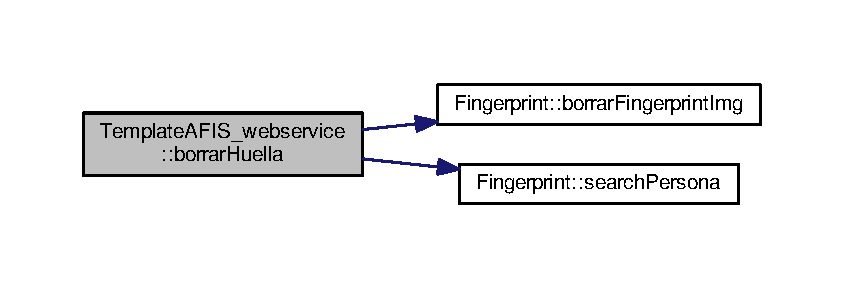
\includegraphics[width=350pt]{classTemplateAFIS__webservice_ac3575e5ecd80a7847c2ecda152778e38_cgraph}
\end{center}
\end{figure}
\hypertarget{classTemplateAFIS__webservice_a5491ba1e8737a0adea2527fcbbc428af}{}\label{classTemplateAFIS__webservice_a5491ba1e8737a0adea2527fcbbc428af} 
\index{Template\+A\+F\+I\+S\+\_\+webservice@{Template\+A\+F\+I\+S\+\_\+webservice}!comprobar@{comprobar}}
\index{comprobar@{comprobar}!Template\+A\+F\+I\+S\+\_\+webservice@{Template\+A\+F\+I\+S\+\_\+webservice}}
\subsubsection{\texorpdfstring{comprobar()}{comprobar()}}
{\footnotesize\ttfamily bool Template\+A\+F\+I\+S\+\_\+webservice\+::comprobar (\begin{DoxyParamCaption}\item[{string}]{usuario,  }\item[{string}]{password }\end{DoxyParamCaption})}



Comprobar\+: Comprueba que haga login. 


\begin{DoxyParams}{Parámetros}
{\em usuario} & Usuario U\+RE \\
\hline
{\em password} & Password U\+RE \\
\hline
\end{DoxyParams}
\begin{DoxyReturn}{Devuelve}
Estado de login.
\end{DoxyReturn}
Método comprobar\+: Comprueba si un usuario puede hacer login, en el Webservice de Open\+E\+RP.

O\+P\+T\+I\+M\+I\+Z\+AR\+: Método debe borrarse no se utiliza 

Definición en la línea 1579 del archivo Template\+A\+F\+I\+S.\+cpp.



Hace referencia a Gui\+Ws\+Open\+Erp\+::\+Inicializar(), Fingerprint\+::is\+U\+R\+E() y Fingerprint\+::\+U\+RL.

Gráfico de llamadas para esta función\+:\nopagebreak
\begin{figure}[H]
\begin{center}
\leavevmode
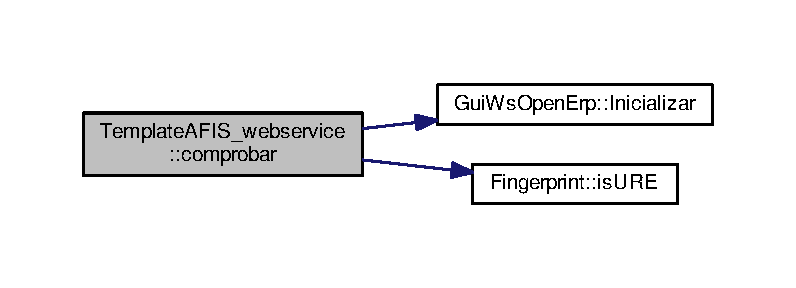
\includegraphics[width=350pt]{classTemplateAFIS__webservice_a5491ba1e8737a0adea2527fcbbc428af_cgraph}
\end{center}
\end{figure}
\hypertarget{classTemplateAFIS__webservice_a32fefd35ad3d702984aa442f4407515d}{}\label{classTemplateAFIS__webservice_a32fefd35ad3d702984aa442f4407515d} 
\index{Template\+A\+F\+I\+S\+\_\+webservice@{Template\+A\+F\+I\+S\+\_\+webservice}!convert\+\_\+raw\+\_\+jpeg@{convert\+\_\+raw\+\_\+jpeg}}
\index{convert\+\_\+raw\+\_\+jpeg@{convert\+\_\+raw\+\_\+jpeg}!Template\+A\+F\+I\+S\+\_\+webservice@{Template\+A\+F\+I\+S\+\_\+webservice}}
\subsubsection{\texorpdfstring{convert\+\_\+raw\+\_\+jpeg()}{convert\_raw\_jpeg()}}
{\footnotesize\ttfamily int Template\+A\+F\+I\+S\+\_\+webservice\+::convert\+\_\+raw\+\_\+jpeg (\begin{DoxyParamCaption}\item[{string}]{filename,  }\item[{unsigned char $\ast$}]{raw,  }\item[{int}]{n\+Width,  }\item[{int}]{n\+Height }\end{DoxyParamCaption})\hspace{0.3cm}{\ttfamily [private]}}



Convert\+\_\+raw\+\_\+jpeg. 


\begin{DoxyParams}{Parámetros}
{\em filename} & Donde se guardará la imágen. \\
\hline
{\em raw} & Binario a convertir. \\
\hline
{\em n\+Width} & Ancho de imágen. \\
\hline
{\em n\+Height} & Alto de imágen. \\
\hline
\end{DoxyParams}
\begin{DoxyReturn}{Devuelve}
Estado de conversión.
\end{DoxyReturn}
Método \hyperlink{classTemplateAFIS__webservice}{Template\+A\+F\+I\+S\+\_\+webservice}\+: Realiza las funciones de Identify, Verify y Enroll, y almacena las huellas en la Base de Datos.

Método convert\+\_\+raw\+\_\+jpeg\+: Convierte un binario de imágen a jpeg. 

Definición en la línea 92 del archivo Template\+A\+F\+I\+S.\+cpp.



Hace referencia a bytes\+\_\+per\+\_\+pixel, color\+\_\+space, Imagen\+::n\+Height y Imagen\+::n\+Width.

\hypertarget{classTemplateAFIS__webservice_a5cf955ee6d8a2cca9fa1116906440f41}{}\label{classTemplateAFIS__webservice_a5cf955ee6d8a2cca9fa1116906440f41} 
\index{Template\+A\+F\+I\+S\+\_\+webservice@{Template\+A\+F\+I\+S\+\_\+webservice}!create\+R\+SA@{create\+R\+SA}}
\index{create\+R\+SA@{create\+R\+SA}!Template\+A\+F\+I\+S\+\_\+webservice@{Template\+A\+F\+I\+S\+\_\+webservice}}
\subsubsection{\texorpdfstring{create\+R\+S\+A()}{createRSA()}}
{\footnotesize\ttfamily R\+SA $\ast$ Template\+A\+F\+I\+S\+\_\+webservice\+::create\+R\+SA (\begin{DoxyParamCaption}\item[{unsigned char $\ast$}]{key,  }\item[{int}]{publica }\end{DoxyParamCaption})}



create\+R\+SA 


\begin{DoxyParams}{Parámetros}
{\em key} & Clave \\
\hline
{\em publica} & Si es o no pública \\
\hline
\end{DoxyParams}


Definición en la línea 2463 del archivo Template\+A\+F\+I\+S.\+cpp.

\hypertarget{classTemplateAFIS__webservice_a4da03ee6cb795586858c4a09f3cdc789}{}\label{classTemplateAFIS__webservice_a4da03ee6cb795586858c4a09f3cdc789} 
\index{Template\+A\+F\+I\+S\+\_\+webservice@{Template\+A\+F\+I\+S\+\_\+webservice}!desencriptar\+Privada@{desencriptar\+Privada}}
\index{desencriptar\+Privada@{desencriptar\+Privada}!Template\+A\+F\+I\+S\+\_\+webservice@{Template\+A\+F\+I\+S\+\_\+webservice}}
\subsubsection{\texorpdfstring{desencriptar\+Privada()}{desencriptarPrivada()}}
{\footnotesize\ttfamily string Template\+A\+F\+I\+S\+\_\+webservice\+::desencriptar\+Privada (\begin{DoxyParamCaption}\item[{string}]{encriptado\+\_\+base64 }\end{DoxyParamCaption})}



desencriptar\+Privada 


\begin{DoxyParams}{Parámetros}
{\em encriptado\+\_\+base64} & Nombre de archivo a abrir \\
\hline
\end{DoxyParams}


Definición en la línea 2538 del archivo Template\+A\+F\+I\+S.\+cpp.

\hypertarget{classTemplateAFIS__webservice_aeb75c2999e3b58cbf800b9f9ffea082c}{}\label{classTemplateAFIS__webservice_aeb75c2999e3b58cbf800b9f9ffea082c} 
\index{Template\+A\+F\+I\+S\+\_\+webservice@{Template\+A\+F\+I\+S\+\_\+webservice}!get\+Datos\+Huella@{get\+Datos\+Huella}}
\index{get\+Datos\+Huella@{get\+Datos\+Huella}!Template\+A\+F\+I\+S\+\_\+webservice@{Template\+A\+F\+I\+S\+\_\+webservice}}
\subsubsection{\texorpdfstring{get\+Datos\+Huella()}{getDatosHuella()}}
{\footnotesize\ttfamily void Template\+A\+F\+I\+S\+\_\+webservice\+::get\+Datos\+Huella (\begin{DoxyParamCaption}\item[{xmlrpc\+\_\+env $\ast$}]{env,  }\item[{string}]{usuario,  }\item[{string}]{password,  }\item[{string}]{cedula,  }\item[{xmlrpc\+\_\+value $\ast$\&}]{my\+ArrayP }\end{DoxyParamCaption})}



Get Datos Huella. 


\begin{DoxyParams}{Parámetros}
{\em env} & Variable X\+M\+L\+R\+PC de ambiente \\
\hline
{\em usuario} & Login \\
\hline
{\em password} & Password \\
\hline
{\em cedula} & Cédula \\
\hline
{\em my\+ArrayP} & Variable X\+M\+L\+R\+PC que volverá con los valores\\
\hline
\end{DoxyParams}
Método get\+Datos\+Huella (X\+M\+L\+R\+PC)\+: Recibe el usuario, password y cédula. Verifica que el usuario tenga permisos, y pide los datos de la huella en base a la mano, dedo, persona. Devuelve el dedo y la mano, de cada huella.

O\+P\+T\+I\+M\+I\+Z\+AR\+: Método no se utiliza debe borrarse 

Definición en la línea 1704 del archivo Template\+A\+F\+I\+S.\+cpp.



Hace referencia a Gui\+Ws\+Open\+Erp\+::get\+Dato\+Huella(), Gui\+Ws\+Open\+Erp\+::\+Inicializar(), Imagen\+::mano, N\+A\+ME y V\+E\+R\+S\+I\+ON.

Gráfico de llamadas para esta función\+:\nopagebreak
\begin{figure}[H]
\begin{center}
\leavevmode
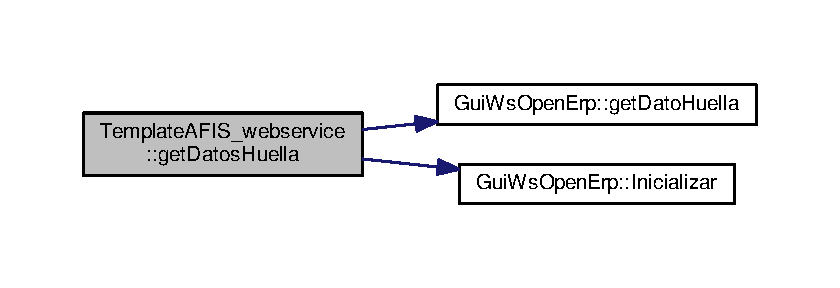
\includegraphics[width=350pt]{classTemplateAFIS__webservice_aeb75c2999e3b58cbf800b9f9ffea082c_cgraph}
\end{center}
\end{figure}
\hypertarget{classTemplateAFIS__webservice_aea7f1b638633ee2440c38573e74d8984}{}\label{classTemplateAFIS__webservice_aea7f1b638633ee2440c38573e74d8984} 
\index{Template\+A\+F\+I\+S\+\_\+webservice@{Template\+A\+F\+I\+S\+\_\+webservice}!get\+Datos\+Id\+Imagen@{get\+Datos\+Id\+Imagen}}
\index{get\+Datos\+Id\+Imagen@{get\+Datos\+Id\+Imagen}!Template\+A\+F\+I\+S\+\_\+webservice@{Template\+A\+F\+I\+S\+\_\+webservice}}
\subsubsection{\texorpdfstring{get\+Datos\+Id\+Imagen()}{getDatosIdImagen()}}
{\footnotesize\ttfamily void Template\+A\+F\+I\+S\+\_\+webservice\+::get\+Datos\+Id\+Imagen (\begin{DoxyParamCaption}\item[{xmlrpc\+\_\+env $\ast$}]{env,  }\item[{string}]{usuario,  }\item[{string}]{password,  }\item[{string}]{cedula,  }\item[{string}]{mano,  }\item[{string}]{id\+\_\+dedo,  }\item[{xmlrpc\+\_\+value $\ast$\&}]{my\+ArrayP }\end{DoxyParamCaption})}



Get Datos Id \hyperlink{classImagen}{Imagen}. 


\begin{DoxyParams}{Parámetros}
{\em env} & Variable X\+M\+L\+R\+PC de ambiente \\
\hline
{\em usuario} & Login \\
\hline
{\em password} & Password \\
\hline
{\em cedula} & Cédula \\
\hline
{\em mano} & Mano \\
\hline
{\em id\+\_\+dedo} & Dedo \\
\hline
{\em my\+ArrayP} & Variable X\+M\+L\+R\+PC que volverá con los valores\\
\hline
\end{DoxyParams}
Método get\+Datos\+Id\+Imagen (X\+M\+L\+R\+PC)\+: Recibe el usuario, password, cédula, mano e id\+\_\+dedo. Devuelve el ID \hyperlink{classImagen}{Imagen}. 

Definición en la línea 2076 del archivo Template\+A\+F\+I\+S.\+cpp.



Hace referencia a N\+A\+ME, Fingerprint\+::read\+Fingerprint(), Fingerprint\+::search\+Persona(), Fingerprint\+::\+U\+RL y V\+E\+R\+S\+I\+ON.

Gráfico de llamadas para esta función\+:\nopagebreak
\begin{figure}[H]
\begin{center}
\leavevmode
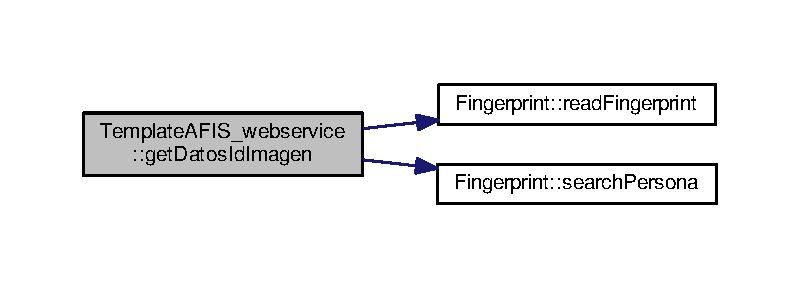
\includegraphics[width=350pt]{classTemplateAFIS__webservice_aea7f1b638633ee2440c38573e74d8984_cgraph}
\end{center}
\end{figure}
\hypertarget{classTemplateAFIS__webservice_a096dfa38545612233dbb64006b01f3e3}{}\label{classTemplateAFIS__webservice_a096dfa38545612233dbb64006b01f3e3} 
\index{Template\+A\+F\+I\+S\+\_\+webservice@{Template\+A\+F\+I\+S\+\_\+webservice}!get\+Datos\+Persona@{get\+Datos\+Persona}}
\index{get\+Datos\+Persona@{get\+Datos\+Persona}!Template\+A\+F\+I\+S\+\_\+webservice@{Template\+A\+F\+I\+S\+\_\+webservice}}
\subsubsection{\texorpdfstring{get\+Datos\+Persona()}{getDatosPersona()}}
{\footnotesize\ttfamily void Template\+A\+F\+I\+S\+\_\+webservice\+::get\+Datos\+Persona (\begin{DoxyParamCaption}\item[{xmlrpc\+\_\+env $\ast$}]{env,  }\item[{string}]{usuario,  }\item[{string}]{password,  }\item[{string}]{cedula,  }\item[{xmlrpc\+\_\+value $\ast$\&}]{my\+ArrayP }\end{DoxyParamCaption})}



Get Datos Persona. 


\begin{DoxyParams}{Parámetros}
{\em env} & Variable X\+M\+L\+R\+PC de ambiente \\
\hline
{\em usuario} & Login \\
\hline
{\em password} & Password \\
\hline
{\em cedula} & Cédula \\
\hline
{\em my\+ArrayP} & Variable X\+M\+L\+R\+PC que volverá con los valores\\
\hline
\end{DoxyParams}
Método get\+Datos\+Persona (X\+M\+L\+R\+PC)\+: Recibe el usuario, password y cédula. Devuelve el nombre y la cédula de la persona. 

Definición en la línea 1868 del archivo Template\+A\+F\+I\+S.\+cpp.



Hace referencia a Gui\+Ws\+Open\+Erp\+::\+Get\+Dato\+Persona(), Gui\+Ws\+Open\+Erp\+::\+Inicializar(), N\+A\+ME y V\+E\+R\+S\+I\+ON.

Gráfico de llamadas para esta función\+:\nopagebreak
\begin{figure}[H]
\begin{center}
\leavevmode
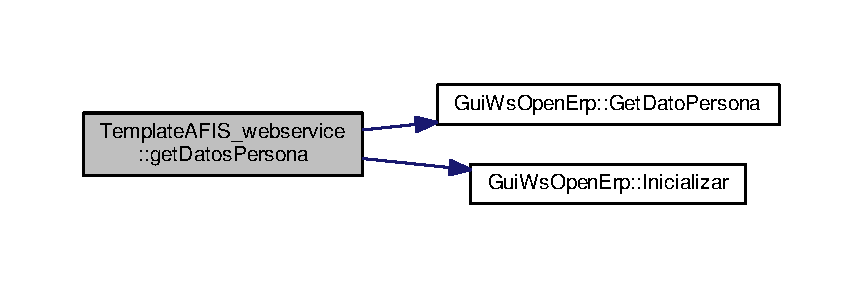
\includegraphics[width=350pt]{classTemplateAFIS__webservice_a096dfa38545612233dbb64006b01f3e3_cgraph}
\end{center}
\end{figure}
\hypertarget{classTemplateAFIS__webservice_adc47efe142e56d2899f8eb8da72ab8eb}{}\label{classTemplateAFIS__webservice_adc47efe142e56d2899f8eb8da72ab8eb} 
\index{Template\+A\+F\+I\+S\+\_\+webservice@{Template\+A\+F\+I\+S\+\_\+webservice}!get\+Datos\+Persona\+O\+B\+PP@{get\+Datos\+Persona\+O\+B\+PP}}
\index{get\+Datos\+Persona\+O\+B\+PP@{get\+Datos\+Persona\+O\+B\+PP}!Template\+A\+F\+I\+S\+\_\+webservice@{Template\+A\+F\+I\+S\+\_\+webservice}}
\subsubsection{\texorpdfstring{get\+Datos\+Persona\+O\+B\+P\+P()}{getDatosPersonaOBPP()}}
{\footnotesize\ttfamily void Template\+A\+F\+I\+S\+\_\+webservice\+::get\+Datos\+Persona\+O\+B\+PP (\begin{DoxyParamCaption}\item[{xmlrpc\+\_\+env $\ast$}]{env,  }\item[{string}]{usuario,  }\item[{string}]{password,  }\item[{string}]{codigo\+\_\+obpp,  }\item[{xmlrpc\+\_\+value $\ast$\&}]{my\+ArrayP }\end{DoxyParamCaption})}



Get Datos Persona O\+B\+PP. 


\begin{DoxyParams}{Parámetros}
{\em env} & Variable X\+M\+L\+R\+PC de ambiente \\
\hline
{\em usuario} & Login \\
\hline
{\em password} & Password \\
\hline
{\em codigo\+\_\+obpp} & Código O\+B\+PP \\
\hline
{\em my\+ArrayP} & Variable X\+M\+L\+R\+PC que volverá con los valores\\
\hline
\end{DoxyParams}
Método get\+Datos\+Persona\+O\+B\+PP (X\+M\+L\+R\+PC)\+: Recibe el usuario, password y codigo\+\_\+obpp. Devuelve el nombre y la cédula de cada persona perteneciente a esa obpp. 

Definición en la línea 1799 del archivo Template\+A\+F\+I\+S.\+cpp.



Hace referencia a Gui\+Ws\+Open\+Erp\+::\+Get\+Persona\+By\+O\+B\+P\+P(), Gui\+Ws\+Open\+Erp\+::\+Inicializar(), N\+A\+ME y V\+E\+R\+S\+I\+ON.

Gráfico de llamadas para esta función\+:\nopagebreak
\begin{figure}[H]
\begin{center}
\leavevmode
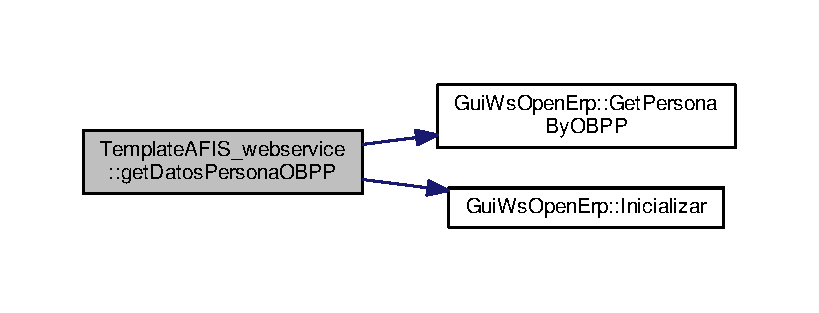
\includegraphics[width=350pt]{classTemplateAFIS__webservice_adc47efe142e56d2899f8eb8da72ab8eb_cgraph}
\end{center}
\end{figure}
\hypertarget{classTemplateAFIS__webservice_a88c4dc259776908b70505380256b68f8}{}\label{classTemplateAFIS__webservice_a88c4dc259776908b70505380256b68f8} 
\index{Template\+A\+F\+I\+S\+\_\+webservice@{Template\+A\+F\+I\+S\+\_\+webservice}!get\+Datos\+Persona\+Verificacion@{get\+Datos\+Persona\+Verificacion}}
\index{get\+Datos\+Persona\+Verificacion@{get\+Datos\+Persona\+Verificacion}!Template\+A\+F\+I\+S\+\_\+webservice@{Template\+A\+F\+I\+S\+\_\+webservice}}
\subsubsection{\texorpdfstring{get\+Datos\+Persona\+Verificacion()}{getDatosPersonaVerificacion()}}
{\footnotesize\ttfamily void Template\+A\+F\+I\+S\+\_\+webservice\+::get\+Datos\+Persona\+Verificacion (\begin{DoxyParamCaption}\item[{xmlrpc\+\_\+env $\ast$}]{env,  }\item[{string}]{usuario,  }\item[{string}]{password,  }\item[{string}]{cedula,  }\item[{xmlrpc\+\_\+value $\ast$\&}]{my\+ArrayP }\end{DoxyParamCaption})}



Get Datos Persona Verificacion. 


\begin{DoxyParams}{Parámetros}
{\em env} & Variable X\+M\+L\+R\+PC de ambiente \\
\hline
{\em usuario} & Login \\
\hline
{\em password} & Password \\
\hline
{\em cedula} & Cédula \\
\hline
{\em my\+ArrayP} & Variable X\+M\+L\+R\+PC que volverá con los valores\\
\hline
\end{DoxyParams}
Método get\+Datos\+Persona\+Verificacion (X\+M\+L\+R\+PC)\+: Recibe el usuario, password y cédula. Devuelve el nombre obpp a la que pertenece, código S\+I\+T\+UR, la cédula de la persona y nombre de la persona. 

Definición en la línea 1954 del archivo Template\+A\+F\+I\+S.\+cpp.



Hace referencia a Gui\+Ws\+Open\+Erp\+::get\+Dato\+Persona\+Verificacion(), Gui\+Ws\+Open\+Erp\+::\+Inicializar(), N\+A\+ME y V\+E\+R\+S\+I\+ON.

Gráfico de llamadas para esta función\+:\nopagebreak
\begin{figure}[H]
\begin{center}
\leavevmode
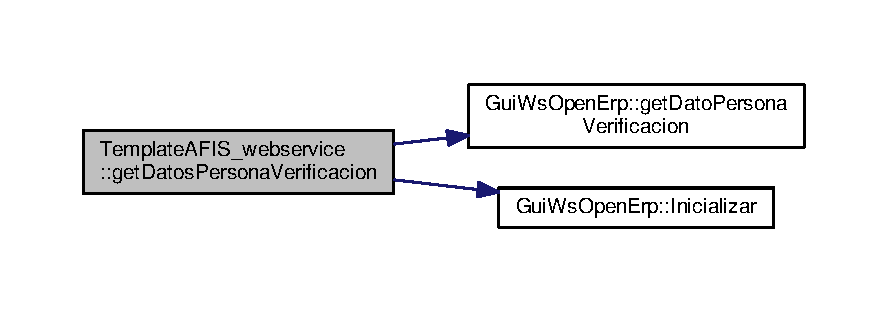
\includegraphics[width=350pt]{classTemplateAFIS__webservice_a88c4dc259776908b70505380256b68f8_cgraph}
\end{center}
\end{figure}
\hypertarget{classTemplateAFIS__webservice_a4842d911ed73f5c33bf5150a6e3bcad4}{}\label{classTemplateAFIS__webservice_a4842d911ed73f5c33bf5150a6e3bcad4} 
\index{Template\+A\+F\+I\+S\+\_\+webservice@{Template\+A\+F\+I\+S\+\_\+webservice}!Get\+Fast\+Mode@{Get\+Fast\+Mode}}
\index{Get\+Fast\+Mode@{Get\+Fast\+Mode}!Template\+A\+F\+I\+S\+\_\+webservice@{Template\+A\+F\+I\+S\+\_\+webservice}}
\subsubsection{\texorpdfstring{Get\+Fast\+Mode()}{GetFastMode()}}
{\footnotesize\ttfamily int Template\+A\+F\+I\+S\+\_\+webservice\+::\+Get\+Fast\+Mode (\begin{DoxyParamCaption}{ }\end{DoxyParamCaption})}



Get Fast Mode. 

\begin{DoxyReturn}{Devuelve}
Obtiene el nivel de rapidez para el Matcher, asociado al captahuellas.
\end{DoxyReturn}
Método Get\+Fast\+Mode\+: Obtiene el valor de obtención de la huella, F\+A\+S\+T\+\_\+\+M\+O\+DE Protocolo de S\+U\+P\+R\+E\+MA indicado en el S\+DK 

Definición en la línea 204 del archivo Template\+A\+F\+I\+S.\+cpp.



Hace referencia a U\+F\+M\+\_\+\+Get\+Parameter() y U\+F\+M\+\_\+\+P\+A\+R\+A\+M\+\_\+\+F\+A\+S\+T\+\_\+\+M\+O\+DE.

Gráfico de llamadas para esta función\+:\nopagebreak
\begin{figure}[H]
\begin{center}
\leavevmode
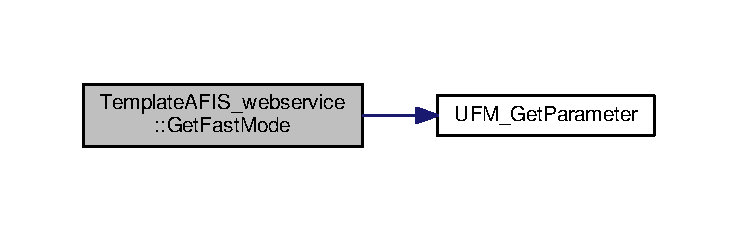
\includegraphics[width=350pt]{classTemplateAFIS__webservice_a4842d911ed73f5c33bf5150a6e3bcad4_cgraph}
\end{center}
\end{figure}
\hypertarget{classTemplateAFIS__webservice_ac6ac32ddd0df850b0e25aa0943c39113}{}\label{classTemplateAFIS__webservice_ac6ac32ddd0df850b0e25aa0943c39113} 
\index{Template\+A\+F\+I\+S\+\_\+webservice@{Template\+A\+F\+I\+S\+\_\+webservice}!Get\+Matcher\+Settings@{Get\+Matcher\+Settings}}
\index{Get\+Matcher\+Settings@{Get\+Matcher\+Settings}!Template\+A\+F\+I\+S\+\_\+webservice@{Template\+A\+F\+I\+S\+\_\+webservice}}
\subsubsection{\texorpdfstring{Get\+Matcher\+Settings()}{GetMatcherSettings()}}
{\footnotesize\ttfamily void Template\+A\+F\+I\+S\+\_\+webservice\+::\+Get\+Matcher\+Settings (\begin{DoxyParamCaption}{ }\end{DoxyParamCaption})}



Get Matcher Settings\+: Muestra la configuración del Matcher (Pruebas) 

Método Get\+Matcher\+Settings\+: Configuraciones del Matcher. Protocolo de S\+U\+P\+R\+E\+MA indicado en el S\+DK 

Definición en la línea 218 del archivo Template\+A\+F\+I\+S.\+cpp.

\hypertarget{classTemplateAFIS__webservice_a664f93880a7054b22a2b1faaacda95c3}{}\label{classTemplateAFIS__webservice_a664f93880a7054b22a2b1faaacda95c3} 
\index{Template\+A\+F\+I\+S\+\_\+webservice@{Template\+A\+F\+I\+S\+\_\+webservice}!Get\+Security\+Level@{Get\+Security\+Level}}
\index{Get\+Security\+Level@{Get\+Security\+Level}!Template\+A\+F\+I\+S\+\_\+webservice@{Template\+A\+F\+I\+S\+\_\+webservice}}
\subsubsection{\texorpdfstring{Get\+Security\+Level()}{GetSecurityLevel()}}
{\footnotesize\ttfamily int Template\+A\+F\+I\+S\+\_\+webservice\+::\+Get\+Security\+Level (\begin{DoxyParamCaption}{ }\end{DoxyParamCaption})}



Get Security Level. 

\begin{DoxyReturn}{Devuelve}
Obtiene el nivel de seguridad para el Matcher, asociado al captahuellas.
\end{DoxyReturn}
Método Get\+Security\+Level\+: Establece el nivel de seguridad. Protocolo de S\+U\+P\+R\+E\+MA indicado en el S\+DK 

Definición en la línea 190 del archivo Template\+A\+F\+I\+S.\+cpp.



Hace referencia a U\+F\+M\+\_\+\+Get\+Parameter() y U\+F\+M\+\_\+\+P\+A\+R\+A\+M\+\_\+\+S\+E\+C\+U\+R\+I\+T\+Y\+\_\+\+L\+E\+V\+EL.

Gráfico de llamadas para esta función\+:\nopagebreak
\begin{figure}[H]
\begin{center}
\leavevmode
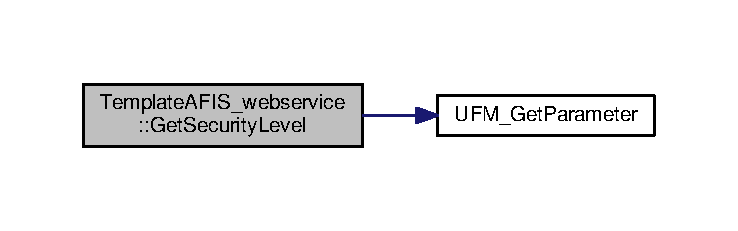
\includegraphics[width=350pt]{classTemplateAFIS__webservice_a664f93880a7054b22a2b1faaacda95c3_cgraph}
\end{center}
\end{figure}
\hypertarget{classTemplateAFIS__webservice_a11ad395942529648ef3a9ddf43df3262}{}\label{classTemplateAFIS__webservice_a11ad395942529648ef3a9ddf43df3262} 
\index{Template\+A\+F\+I\+S\+\_\+webservice@{Template\+A\+F\+I\+S\+\_\+webservice}!get\+Usuario@{get\+Usuario}}
\index{get\+Usuario@{get\+Usuario}!Template\+A\+F\+I\+S\+\_\+webservice@{Template\+A\+F\+I\+S\+\_\+webservice}}
\subsubsection{\texorpdfstring{get\+Usuario()}{getUsuario()}}
{\footnotesize\ttfamily void Template\+A\+F\+I\+S\+\_\+webservice\+::get\+Usuario (\begin{DoxyParamCaption}\item[{xmlrpc\+\_\+env $\ast$}]{env,  }\item[{string}]{usuario,  }\item[{string}]{password,  }\item[{xmlrpc\+\_\+value $\ast$\&}]{my\+ArrayP }\end{DoxyParamCaption})}



Get Usuario. 


\begin{DoxyParams}{Parámetros}
{\em env} & Variable X\+M\+L\+R\+PC de ambiente \\
\hline
{\em usuario} & Login \\
\hline
{\em password} & Password \\
\hline
{\em my\+ArrayP} & Variable X\+M\+L\+R\+PC que volverá con los valores\\
\hline
\end{DoxyParams}
Método get\+Usuario (X\+M\+L\+R\+PC)\+: Recibe el usuario y el password. Devuelve el parámetros verificacion, para validar un usuario.

O\+P\+T\+I\+M\+I\+Z\+AR\+: Método no se utiliza debe borrarse 

Definición en la línea 1640 del archivo Template\+A\+F\+I\+S.\+cpp.



Hace referencia a Gui\+Ws\+Open\+Erp\+::\+Inicializar(), N\+A\+ME y V\+E\+R\+S\+I\+ON.

Gráfico de llamadas para esta función\+:\nopagebreak
\begin{figure}[H]
\begin{center}
\leavevmode
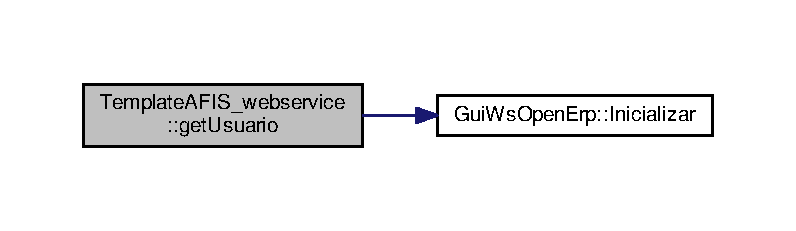
\includegraphics[width=350pt]{classTemplateAFIS__webservice_a11ad395942529648ef3a9ddf43df3262_cgraph}
\end{center}
\end{figure}
\hypertarget{classTemplateAFIS__webservice_acd9566662ac9e462b438e21c788d5f48}{}\label{classTemplateAFIS__webservice_acd9566662ac9e462b438e21c788d5f48} 
\index{Template\+A\+F\+I\+S\+\_\+webservice@{Template\+A\+F\+I\+S\+\_\+webservice}!get\+Web\+Service\+G\+U\+I\+Open\+E\+RP@{get\+Web\+Service\+G\+U\+I\+Open\+E\+RP}}
\index{get\+Web\+Service\+G\+U\+I\+Open\+E\+RP@{get\+Web\+Service\+G\+U\+I\+Open\+E\+RP}!Template\+A\+F\+I\+S\+\_\+webservice@{Template\+A\+F\+I\+S\+\_\+webservice}}
\subsubsection{\texorpdfstring{get\+Web\+Service\+G\+U\+I\+Open\+E\+R\+P()}{getWebServiceGUIOpenERP()}}
{\footnotesize\ttfamily void Template\+A\+F\+I\+S\+\_\+webservice\+::get\+Web\+Service\+G\+U\+I\+Open\+E\+RP (\begin{DoxyParamCaption}\item[{string}]{usuario,  }\item[{string}]{pass,  }\item[{\hyperlink{classGuiWsOpenErp}{Gui\+Ws\+Open\+Erp} $\ast$\&}]{fing }\end{DoxyParamCaption})}



Get Webservice G\+UI Open\+E\+RP\+: Objeto que hace conexión con el Webservice de Open\+E\+RP. 


\begin{DoxyParams}{Parámetros}
{\em usuario} & Usuario U\+RE \\
\hline
{\em pass} & Password U\+RE \\
\hline
{\em fing} & Objeto \hyperlink{classGuiWsOpenErp}{Gui\+Ws\+Open\+Erp}\\
\hline
\end{DoxyParams}
Método get\+Web\+Service\+G\+U\+I\+Open\+E\+RP\+: Obtiene un objeto para realizar transacciones X\+M\+L\+R\+PC. 

Definición en la línea 2327 del archivo Template\+A\+F\+I\+S.\+cpp.



Hace referencia a N\+U\+M\+\_\+\+W\+E\+B\+S\+E\+R\+V\+I\+CE.

\hypertarget{classTemplateAFIS__webservice_a9c035f2b4dc64d540ae6e4e9161e0fa3}{}\label{classTemplateAFIS__webservice_a9c035f2b4dc64d540ae6e4e9161e0fa3} 
\index{Template\+A\+F\+I\+S\+\_\+webservice@{Template\+A\+F\+I\+S\+\_\+webservice}!get\+Web\+Service\+Open\+E\+RP@{get\+Web\+Service\+Open\+E\+RP}}
\index{get\+Web\+Service\+Open\+E\+RP@{get\+Web\+Service\+Open\+E\+RP}!Template\+A\+F\+I\+S\+\_\+webservice@{Template\+A\+F\+I\+S\+\_\+webservice}}
\subsubsection{\texorpdfstring{get\+Web\+Service\+Open\+E\+R\+P()}{getWebServiceOpenERP()}}
{\footnotesize\ttfamily void Template\+A\+F\+I\+S\+\_\+webservice\+::get\+Web\+Service\+Open\+E\+RP (\begin{DoxyParamCaption}\item[{string}]{usuario,  }\item[{string}]{pass,  }\item[{\hyperlink{classFingerprint}{Fingerprint} $\ast$\&}]{fing }\end{DoxyParamCaption})}



Get Webservice Open\+E\+RP\+: Objeto que hace conexión con el Webservice de Open\+E\+RP. 


\begin{DoxyParams}{Parámetros}
{\em usuario} & Usuario U\+RE \\
\hline
{\em pass} & Password U\+RE \\
\hline
{\em fing} & Objeto \hyperlink{classFingerprint}{Fingerprint}\\
\hline
\end{DoxyParams}
Método get\+Web\+Service\+Open\+E\+RP\+: Obtiene un objeto para realizar transacciones X\+M\+L\+R\+PC. 

Definición en la línea 2295 del archivo Template\+A\+F\+I\+S.\+cpp.



Hace referencia a N\+U\+M\+\_\+\+W\+E\+B\+S\+E\+R\+V\+I\+CE.

\hypertarget{classTemplateAFIS__webservice_aa4536bcf883164f6c3c6d9dcb8744c7f}{}\label{classTemplateAFIS__webservice_aa4536bcf883164f6c3c6d9dcb8744c7f} 
\index{Template\+A\+F\+I\+S\+\_\+webservice@{Template\+A\+F\+I\+S\+\_\+webservice}!guardar\+Incidencia@{guardar\+Incidencia}}
\index{guardar\+Incidencia@{guardar\+Incidencia}!Template\+A\+F\+I\+S\+\_\+webservice@{Template\+A\+F\+I\+S\+\_\+webservice}}
\subsubsection{\texorpdfstring{guardar\+Incidencia()}{guardarIncidencia()}}
{\footnotesize\ttfamily int Template\+A\+F\+I\+S\+\_\+webservice\+::guardar\+Incidencia (\begin{DoxyParamCaption}\item[{string}]{usuario,  }\item[{string}]{password,  }\item[{string}]{id\+\_\+persona,  }\item[{string}]{id\+\_\+dedo,  }\item[{string}]{mano,  }\item[{string}]{id\+\_\+proyecto }\end{DoxyParamCaption})}



Definición en la línea 654 del archivo Template\+A\+F\+I\+S.\+cpp.



Hace referencia a Fingerprint\+::dbname, estado\+\_\+proyecto\+::set\+\_\+variables(), Fingerprint\+::\+U\+RL y estado\+\_\+proyecto\+::validacion\+\_\+incidencias\+\_\+huella().

Gráfico de llamadas para esta función\+:\nopagebreak
\begin{figure}[H]
\begin{center}
\leavevmode
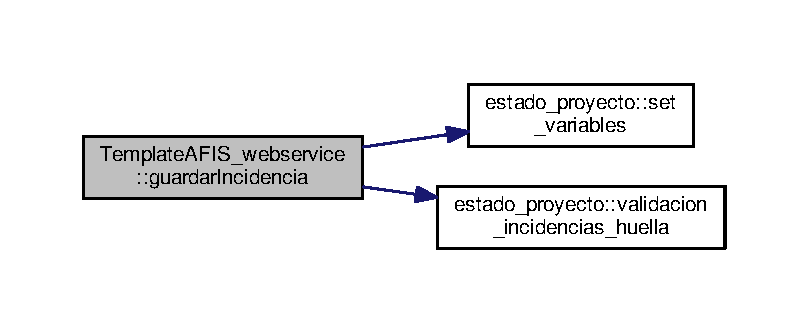
\includegraphics[width=350pt]{classTemplateAFIS__webservice_aa4536bcf883164f6c3c6d9dcb8744c7f_cgraph}
\end{center}
\end{figure}
\hypertarget{classTemplateAFIS__webservice_a8698c0f638f3be26a0664edd56038847}{}\label{classTemplateAFIS__webservice_a8698c0f638f3be26a0664edd56038847} 
\index{Template\+A\+F\+I\+S\+\_\+webservice@{Template\+A\+F\+I\+S\+\_\+webservice}!init\+Matcher@{init\+Matcher}}
\index{init\+Matcher@{init\+Matcher}!Template\+A\+F\+I\+S\+\_\+webservice@{Template\+A\+F\+I\+S\+\_\+webservice}}
\subsubsection{\texorpdfstring{init\+Matcher()}{initMatcher()}}
{\footnotesize\ttfamily bool Template\+A\+F\+I\+S\+\_\+webservice\+::init\+Matcher (\begin{DoxyParamCaption}{ }\end{DoxyParamCaption})}



Init Matcher. 

\begin{DoxyReturn}{Devuelve}
Obtiene el estado de inicialización del Matcher. True o False
\end{DoxyReturn}
Método init\+Matcher\+: Inicializa el Matcher. Protocolo de S\+U\+P\+R\+E\+MA indicado en el S\+DK 

Definición en la línea 229 del archivo Template\+A\+F\+I\+S.\+cpp.



Hace referencia a U\+F\+M\+\_\+\+Create(), U\+F\+M\+\_\+\+Get\+Error\+String(), U\+F\+M\+\_\+\+OK y U\+F\+M\+\_\+\+S\+T\+A\+T\+US.

Gráfico de llamadas para esta función\+:\nopagebreak
\begin{figure}[H]
\begin{center}
\leavevmode
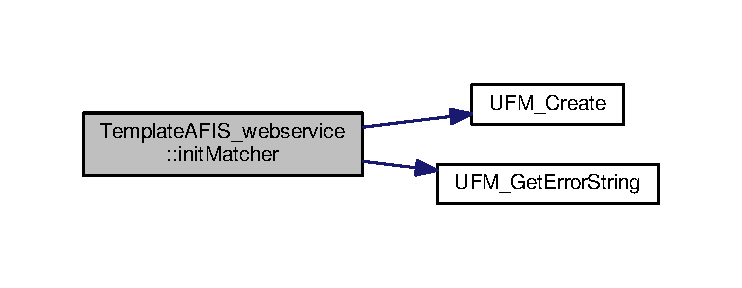
\includegraphics[width=350pt]{classTemplateAFIS__webservice_a8698c0f638f3be26a0664edd56038847_cgraph}
\end{center}
\end{figure}
\hypertarget{classTemplateAFIS__webservice_a1fb45563a560d59202d2d051fa649798}{}\label{classTemplateAFIS__webservice_a1fb45563a560d59202d2d051fa649798} 
\index{Template\+A\+F\+I\+S\+\_\+webservice@{Template\+A\+F\+I\+S\+\_\+webservice}!is\+\_\+base64@{is\+\_\+base64}}
\index{is\+\_\+base64@{is\+\_\+base64}!Template\+A\+F\+I\+S\+\_\+webservice@{Template\+A\+F\+I\+S\+\_\+webservice}}
\subsubsection{\texorpdfstring{is\+\_\+base64()}{is\_base64()}}
{\footnotesize\ttfamily bool Template\+A\+F\+I\+S\+\_\+webservice\+::is\+\_\+base64 (\begin{DoxyParamCaption}\item[{unsigned char}]{c }\end{DoxyParamCaption})}



is\+\_\+base64 


\begin{DoxyParams}{Parámetros}
{\em c} & Caracter base64 \\
\hline
\end{DoxyParams}


Definición en la línea 2375 del archivo Template\+A\+F\+I\+S.\+cpp.

\hypertarget{classTemplateAFIS__webservice_a432d8a18012883bacddf5f9db4b58b69}{}\label{classTemplateAFIS__webservice_a432d8a18012883bacddf5f9db4b58b69} 
\index{Template\+A\+F\+I\+S\+\_\+webservice@{Template\+A\+F\+I\+S\+\_\+webservice}!leer\+Todo\+Un\+Archivo@{leer\+Todo\+Un\+Archivo}}
\index{leer\+Todo\+Un\+Archivo@{leer\+Todo\+Un\+Archivo}!Template\+A\+F\+I\+S\+\_\+webservice@{Template\+A\+F\+I\+S\+\_\+webservice}}
\subsubsection{\texorpdfstring{leer\+Todo\+Un\+Archivo()}{leerTodoUnArchivo()}}
{\footnotesize\ttfamily string Template\+A\+F\+I\+S\+\_\+webservice\+::leer\+Todo\+Un\+Archivo (\begin{DoxyParamCaption}\item[{string}]{nombre\+\_\+archivo }\end{DoxyParamCaption})}



leer\+Todo\+Un\+Archivo 


\begin{DoxyParams}{Parámetros}
{\em nombre\+\_\+archivo} & Nombre de archivo a abrir \\
\hline
\end{DoxyParams}


Definición en la línea 2519 del archivo Template\+A\+F\+I\+S.\+cpp.

\hypertarget{classTemplateAFIS__webservice_a5fc2884ea75075e40a6056440021f27d}{}\label{classTemplateAFIS__webservice_a5fc2884ea75075e40a6056440021f27d} 
\index{Template\+A\+F\+I\+S\+\_\+webservice@{Template\+A\+F\+I\+S\+\_\+webservice}!On\+Enroll@{On\+Enroll}}
\index{On\+Enroll@{On\+Enroll}!Template\+A\+F\+I\+S\+\_\+webservice@{Template\+A\+F\+I\+S\+\_\+webservice}}
\subsubsection{\texorpdfstring{On\+Enroll()}{OnEnroll()}}
{\footnotesize\ttfamily int Template\+A\+F\+I\+S\+\_\+webservice\+::\+On\+Enroll (\begin{DoxyParamCaption}\item[{string}]{usuario,  }\item[{string}]{password,  }\item[{string}]{id\+\_\+persona,  }\item[{string}]{id\+\_\+dedo,  }\item[{string}]{mano,  }\item[{string}]{hash,  }\item[{unsigned char $\ast$\&}]{m\+\_\+template,  }\item[{int}]{m\+\_\+template\+\_\+size,  }\item[{unsigned char $\ast$\&}]{p\+Image\+Data,  }\item[{int}]{n\+Width,  }\item[{int}]{n\+Height,  }\item[{string \&}]{id\+\_\+persona\+\_\+out,  }\item[{string \&}]{id\+\_\+dedo\+\_\+out,  }\item[{string \&}]{mano\+\_\+out }\end{DoxyParamCaption})}



On Enroll. 


\begin{DoxyParams}{Parámetros}
{\em usuario} & Usuario U\+RE \\
\hline
{\em password} & Password U\+RE \\
\hline
{\em id\+\_\+persona} & Cédula persona \\
\hline
{\em id\+\_\+dedo} & Dedo \\
\hline
{\em mano} & Mano \\
\hline
{\em hash} & Hash \\
\hline
{\em m\+\_\+template} & Huella a guardar \\
\hline
{\em m\+\_\+template\+\_\+size} & Tamaño de huella a guardar \\
\hline
{\em p\+Image\+Data} & Imágen de huella a guardar \\
\hline
{\em n\+Width} & Ancho de imágen de huella a guardar \\
\hline
{\em n\+Height} & Alto de imágen de huella a guardar \\
\hline
{\em id\+\_\+persona\+\_\+out} & Si la huella está repetida, Cédula de la persona donde está repetida. \\
\hline
{\em id\+\_\+dedo\+\_\+out} & Si la huella está repetida, Dedo de la persona donde está repetida. \\
\hline
{\em mano\+\_\+out} & Si la huella está repetida, Mano de la persona donde está repetida. \\
\hline
\end{DoxyParams}
\begin{DoxyReturn}{Devuelve}
Estado de guardado.
\end{DoxyReturn}
Método On\+Enroll\+: Guarda la huella en Odoo. Permite relacionar el Captahuellas con Odoo. 

Definición en la línea 353 del archivo Template\+A\+F\+I\+S.\+cpp.



Hace referencia a Fingerprint\+::actualizar\+Fingerprint\+Web\+Service(), Fingerprint\+::insertar\+Fingerprint\+Web\+Service(), N\+A\+ME, Imagen\+::n\+Height, Imagen\+::n\+Width, Fingerprint\+::search\+Fingerprint(), Fingerprint\+::search\+Persona(), Fingerprint\+::\+U\+RL y V\+E\+R\+S\+I\+ON.

Gráfico de llamadas para esta función\+:\nopagebreak
\begin{figure}[H]
\begin{center}
\leavevmode
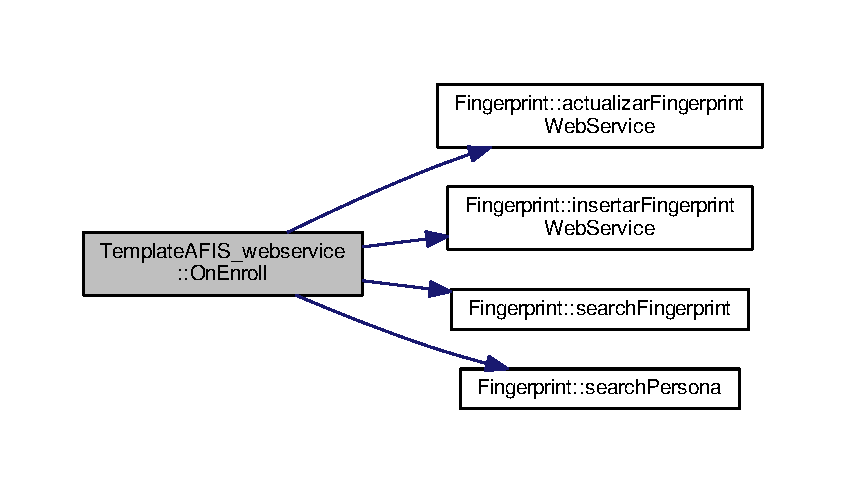
\includegraphics[width=350pt]{classTemplateAFIS__webservice_a5fc2884ea75075e40a6056440021f27d_cgraph}
\end{center}
\end{figure}
\hypertarget{classTemplateAFIS__webservice_a40bd372e1a5b01d9bc2b4e1898be967f}{}\label{classTemplateAFIS__webservice_a40bd372e1a5b01d9bc2b4e1898be967f} 
\index{Template\+A\+F\+I\+S\+\_\+webservice@{Template\+A\+F\+I\+S\+\_\+webservice}!On\+Get\+Parameters@{On\+Get\+Parameters}}
\index{On\+Get\+Parameters@{On\+Get\+Parameters}!Template\+A\+F\+I\+S\+\_\+webservice@{Template\+A\+F\+I\+S\+\_\+webservice}}
\subsubsection{\texorpdfstring{On\+Get\+Parameters()}{OnGetParameters()}}
{\footnotesize\ttfamily void Template\+A\+F\+I\+S\+\_\+webservice\+::\+On\+Get\+Parameters (\begin{DoxyParamCaption}{ }\end{DoxyParamCaption})}



On Get Parameters. 

\begin{DoxyReturn}{Devuelve}
Muestra los parámetros del Matcher
\end{DoxyReturn}
Método On\+Get\+Parameters\+: Obtener los parámetros del objeto Matcher. Protocolo de S\+U\+P\+R\+E\+MA indicado en el S\+DK 

Definición en la línea 286 del archivo Template\+A\+F\+I\+S.\+cpp.

\hypertarget{classTemplateAFIS__webservice_ab66286f0a3f0702977a46332d3bce05d}{}\label{classTemplateAFIS__webservice_ab66286f0a3f0702977a46332d3bce05d} 
\index{Template\+A\+F\+I\+S\+\_\+webservice@{Template\+A\+F\+I\+S\+\_\+webservice}!On\+Identify@{On\+Identify}}
\index{On\+Identify@{On\+Identify}!Template\+A\+F\+I\+S\+\_\+webservice@{Template\+A\+F\+I\+S\+\_\+webservice}}
\subsubsection{\texorpdfstring{On\+Identify()}{OnIdentify()}}
{\footnotesize\ttfamily int Template\+A\+F\+I\+S\+\_\+webservice\+::\+On\+Identify (\begin{DoxyParamCaption}\item[{string}]{usuario,  }\item[{string}]{password,  }\item[{unsigned char $\ast$}]{Template,  }\item[{int}]{Template\+Size,  }\item[{string}]{cedula\+\_\+in,  }\item[{string \&}]{cedula,  }\item[{string \&}]{dedo,  }\item[{string \&}]{hand }\end{DoxyParamCaption})}



iteracion\+Identify\+: Identifica usando verificación en cada iteración. Se utiliza con On\+Identify\+Verify (No On\+Identify\+On\+Verify. iteacion\+Identify, no se utiliza en esta versión) 


\begin{DoxyParams}{Parámetros}
{\em estado} & Estado de la verificación \\
\hline
{\em i} & Id de la huella en la Base de Datos \\
\hline
{\em id\+\_\+persona\+\_\+result} & Cédula encontrada \\
\hline
{\em id\+\_\+dedo\+\_\+result} & Dedo encontrado \\
\hline
{\em mano\+\_\+result} & Mano encontrada \\
\hline
{\em id\+\_\+partner} & Id partner a comparar \\
\hline
{\em id\+\_\+dedo} & Dedo a comparar \\
\hline
{\em mano} & Mano a comparar \\
\hline
{\em Template} & Huella a verificar \\
\hline
{\em Template\+Size} & Tamaño de huella a verificar \\
\hline
{\em ufm\+\_\+res} & Estado de la verificación. \\
\hline
{\em b\+Verify\+Succeed} & Verificación exitosa (o no) \\
\hline
\end{DoxyParams}
\begin{DoxyReturn}{Devuelve}
Estado de verificacion. On\+Identify\+Verify\+: Identifica usando verificación en cada iteración. Se utiliza con iteacion\+Identify (On\+Identify\+Verify, no se utiliza en esta versión) 
\end{DoxyReturn}

\begin{DoxyParams}{Parámetros}
{\em usuario} & Usuario U\+RE \\
\hline
{\em password} & Password U\+RE \\
\hline
{\em Template} & Huella a verificar \\
\hline
{\em Template\+Size} & Tamaño de huella a verificar \\
\hline
{\em cedula} & Cédula de la persona a verificar \\
\hline
{\em id\+\_\+dedo} & Dedo de la persona a verificar \\
\hline
{\em mano} & Mano de la persona a verificar \\
\hline
{\em cedula\+\_\+out} & Cédula de la persona encontrada \\
\hline
{\em dedo\+\_\+out} & Dedo de la persona encontrada \\
\hline
{\em hand\+\_\+out} & Mano de la persona encontrada \\
\hline
\end{DoxyParams}
\begin{DoxyReturn}{Devuelve}
Estado de verificacion (Identificación). On\+Identify\+: Identifica usando el método de identificación de Bio\+Suprema 
\end{DoxyReturn}

\begin{DoxyParams}{Parámetros}
{\em usuario} & Usuario U\+RE \\
\hline
{\em password} & Password U\+RE \\
\hline
{\em Template} & Huella a identificar \\
\hline
{\em Template\+Size} & Tamaño de huella a identificar \\
\hline
{\em cedula\+\_\+in} & Cédula de la persona, cuando se va a buscar por estado. \\
\hline
{\em cedula} & Cédula de la persona encontrada. \\
\hline
{\em dedo} & Dedo de la persona encontrada \\
\hline
{\em hand} & Mano de la persona encontrada \\
\hline
\end{DoxyParams}
\begin{DoxyReturn}{Devuelve}
Estado de identificación.
\end{DoxyReturn}
Método iteracion\+Identify\+: Realiza la iteración de identificación de una huella, una por una; esto quiere decir un verify a cada huella. Utiliza el método de verificación de Bio\+Suprema.

Método On\+Identify\+Verify\+: Identifica las huellas una por una. Utiliza el método de verificación de Bio\+Suprema.

Método On\+Identify\+: Identifica una huella contra muchas. Utiliza el método de identificación de Bio\+Suprema. Verifica que el captahuellas esté conectado. Verifica que el usuario de Odoo sea el correcto. 

Definición en la línea 945 del archivo Template\+A\+F\+I\+S.\+cpp.



Hace referencia a Imagen\+::id\+\_\+dedo, Imagen\+::id\+\_\+persona, Imagen\+::mano, N\+A\+ME, Fingerprint\+::read\+Fingerprint(), Fingerprint\+::read\+Vat\+Persona(), Fingerprint\+::search\+Persona(), U\+F\+M\+\_\+\+Get\+Error\+String(), U\+F\+M\+\_\+\+Identify(), U\+F\+M\+\_\+\+OK, U\+F\+M\+\_\+\+S\+T\+A\+T\+US, Fingerprint\+::\+U\+RL y V\+E\+R\+S\+I\+ON.

Gráfico de llamadas para esta función\+:\nopagebreak
\begin{figure}[H]
\begin{center}
\leavevmode
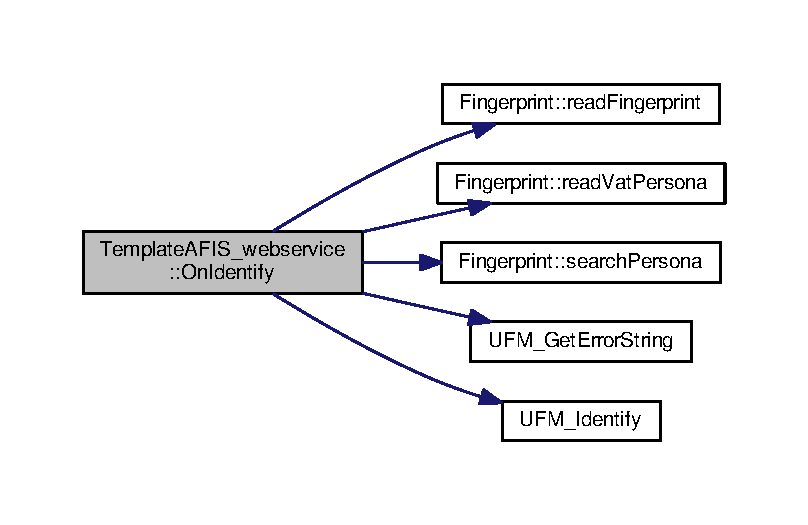
\includegraphics[width=350pt]{classTemplateAFIS__webservice_ab66286f0a3f0702977a46332d3bce05d_cgraph}
\end{center}
\end{figure}
\hypertarget{classTemplateAFIS__webservice_a2c62949a4ec904bfc4571d95d577ddb4}{}\label{classTemplateAFIS__webservice_a2c62949a4ec904bfc4571d95d577ddb4} 
\index{Template\+A\+F\+I\+S\+\_\+webservice@{Template\+A\+F\+I\+S\+\_\+webservice}!On\+Identify\+On\+Verify@{On\+Identify\+On\+Verify}}
\index{On\+Identify\+On\+Verify@{On\+Identify\+On\+Verify}!Template\+A\+F\+I\+S\+\_\+webservice@{Template\+A\+F\+I\+S\+\_\+webservice}}
\subsubsection{\texorpdfstring{On\+Identify\+On\+Verify()}{OnIdentifyOnVerify()}}
{\footnotesize\ttfamily int Template\+A\+F\+I\+S\+\_\+webservice\+::\+On\+Identify\+On\+Verify (\begin{DoxyParamCaption}\item[{string}]{usuario,  }\item[{string}]{password,  }\item[{unsigned char $\ast$\&}]{Template,  }\item[{int}]{Template\+Size,  }\item[{string}]{cedula\+\_\+in,  }\item[{string \&}]{cedula,  }\item[{string \&}]{dedo,  }\item[{string \&}]{hand,  }\item[{string \&}]{situr }\end{DoxyParamCaption})}



On\+Identify\+On\+Verify\+: Identifica usando el método de identificación de Bio\+Suprema. Se utiliza con On\+Verify. Si la verificación falla, llama a este método. 


\begin{DoxyParams}{Parámetros}
{\em usuario} & Usuario U\+RE \\
\hline
{\em password} & Password U\+RE \\
\hline
{\em Template} & Huella a identificar \\
\hline
{\em Template\+Size} & Tamaño de huella a identificar \\
\hline
{\em cedula\+\_\+in} & Cédula de la persona, cuando se va a buscar por estado. \\
\hline
{\em cedula} & Cédula de la persona encontrada. \\
\hline
{\em dedo} & Dedo de la persona encontrada \\
\hline
{\em hand} & Mano de la persona encontrada \\
\hline
{\em situr} & Código S\+I\+T\+UR de la persona encontrada \\
\hline
\end{DoxyParams}
\begin{DoxyReturn}{Devuelve}
Estado de identificación.
\end{DoxyReturn}
O\+P\+T\+I\+M\+I\+Z\+AR\+: Revisar Método On\+Identify\+On\+Verify Revisar Narrativa de S\+I\+N\+CO 

Definición en la línea 1193 del archivo Template\+A\+F\+I\+S.\+cpp.



Hace referencia a Imagen\+::id\+\_\+dedo, Imagen\+::id\+\_\+persona, Imagen\+::mano, N\+A\+ME, Fingerprint\+::read\+Fingerprint(), Fingerprint\+::read\+Vat\+Persona(), Fingerprint\+::search\+Persona(), U\+F\+M\+\_\+\+Get\+Error\+String(), U\+F\+M\+\_\+\+Identify(), U\+F\+M\+\_\+\+OK, U\+F\+M\+\_\+\+S\+T\+A\+T\+US, Fingerprint\+::\+U\+RL y V\+E\+R\+S\+I\+ON.

Gráfico de llamadas para esta función\+:\nopagebreak
\begin{figure}[H]
\begin{center}
\leavevmode
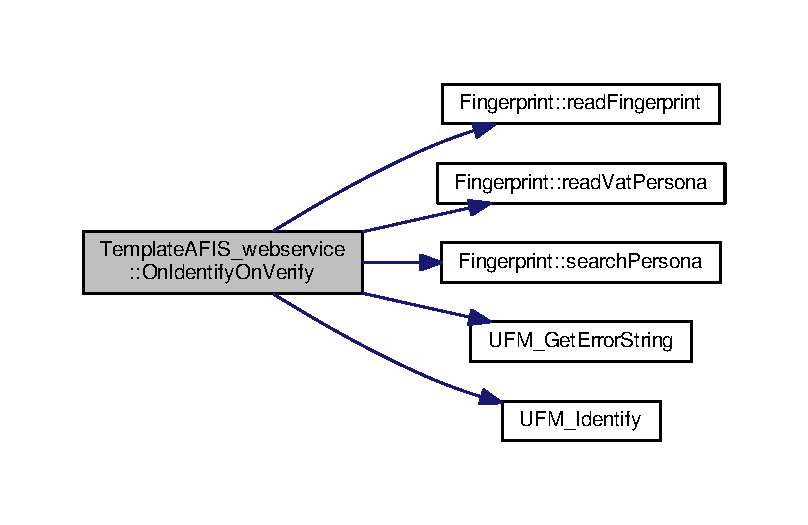
\includegraphics[width=350pt]{classTemplateAFIS__webservice_a2c62949a4ec904bfc4571d95d577ddb4_cgraph}
\end{center}
\end{figure}
\hypertarget{classTemplateAFIS__webservice_aa89af892ebe892d1a92f1e2dad5e998d}{}\label{classTemplateAFIS__webservice_aa89af892ebe892d1a92f1e2dad5e998d} 
\index{Template\+A\+F\+I\+S\+\_\+webservice@{Template\+A\+F\+I\+S\+\_\+webservice}!On\+Set\+Template\+Type@{On\+Set\+Template\+Type}}
\index{On\+Set\+Template\+Type@{On\+Set\+Template\+Type}!Template\+A\+F\+I\+S\+\_\+webservice@{Template\+A\+F\+I\+S\+\_\+webservice}}
\subsubsection{\texorpdfstring{On\+Set\+Template\+Type()}{OnSetTemplateType()}}
{\footnotesize\ttfamily int Template\+A\+F\+I\+S\+\_\+webservice\+::\+On\+Set\+Template\+Type (\begin{DoxyParamCaption}\item[{int}]{value }\end{DoxyParamCaption})}



On Set Template Type. 


\begin{DoxyParams}{Parámetros}
{\em value} & Número de tipo de Template. 1 para S\+U\+P\+R\+E\+MA, 2 para I\+S\+O19794\+\_\+2, 3 para A\+N\+S\+I378 \\
\hline
\end{DoxyParams}
\begin{DoxyReturn}{Devuelve}
Estado luego de establecer el tipo de Template.
\end{DoxyReturn}
Método On\+Set\+Template\+Type\+: Establecer los tipos de template. Protocolo de S\+U\+P\+R\+E\+MA indicado en el S\+DK 

Definición en la línea 300 del archivo Template\+A\+F\+I\+S.\+cpp.



Hace referencia a U\+F\+M\+\_\+\+Set\+Template\+Type(), U\+F\+S\+\_\+\+T\+E\+M\+P\+L\+A\+T\+E\+\_\+\+T\+Y\+P\+E\+\_\+\+A\+N\+S\+I378, U\+F\+S\+\_\+\+T\+E\+M\+P\+L\+A\+T\+E\+\_\+\+T\+Y\+P\+E\+\_\+\+I\+S\+O19794\+\_\+2 y U\+F\+S\+\_\+\+T\+E\+M\+P\+L\+A\+T\+E\+\_\+\+T\+Y\+P\+E\+\_\+\+S\+U\+P\+R\+E\+MA.

Gráfico de llamadas para esta función\+:\nopagebreak
\begin{figure}[H]
\begin{center}
\leavevmode
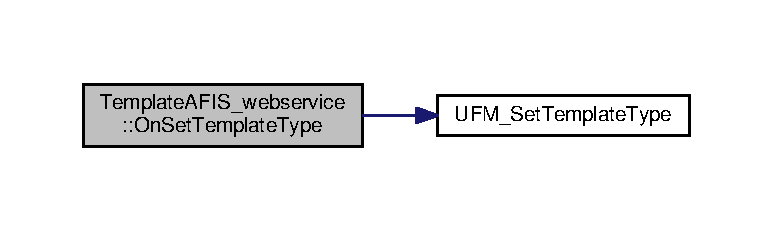
\includegraphics[width=350pt]{classTemplateAFIS__webservice_aa89af892ebe892d1a92f1e2dad5e998d_cgraph}
\end{center}
\end{figure}
\hypertarget{classTemplateAFIS__webservice_ad2d94adf36b56bf3306e52e5e20ecaab}{}\label{classTemplateAFIS__webservice_ad2d94adf36b56bf3306e52e5e20ecaab} 
\index{Template\+A\+F\+I\+S\+\_\+webservice@{Template\+A\+F\+I\+S\+\_\+webservice}!On\+Verify@{On\+Verify}}
\index{On\+Verify@{On\+Verify}!Template\+A\+F\+I\+S\+\_\+webservice@{Template\+A\+F\+I\+S\+\_\+webservice}}
\subsubsection{\texorpdfstring{On\+Verify()}{OnVerify()}}
{\footnotesize\ttfamily int Template\+A\+F\+I\+S\+\_\+webservice\+::\+On\+Verify (\begin{DoxyParamCaption}\item[{string}]{usuario,  }\item[{string}]{password,  }\item[{string}]{id\+\_\+proyecto,  }\item[{string}]{id\+\_\+persona,  }\item[{string}]{id\+\_\+dedo,  }\item[{string}]{mano,  }\item[{unsigned char $\ast$\&}]{Template,  }\item[{int}]{Template\+Size,  }\item[{string \&}]{cedula,  }\item[{string \&}]{dedo,  }\item[{string \&}]{hand,  }\item[{string \&}]{situr }\end{DoxyParamCaption})}



On Verify\+: Verifica una huella. Si la huella no es la verificada, utiliza el Médoto On\+Identify\+On\+Verify, para obtener donde está, obteniendo cedula, dedo, mano y código Situr. 


\begin{DoxyParams}{Parámetros}
{\em usuario} & Usuario U\+RE \\
\hline
{\em password} & Password U\+RE \\
\hline
{\em id\+\_\+persona} & Cédula persona \\
\hline
{\em id\+\_\+dedo} & Dedo \\
\hline
{\em mano} & Mano \\
\hline
{\em Template} & Huella a verificar \\
\hline
{\em Template\+Size} & Tamaño de huella a verificar \\
\hline
{\em cedula} & Si no es la huella, Cédula de la persona donde está la huella. \\
\hline
{\em dedo} & Si no es la huella, Dedo de la persona donde está la huella. \\
\hline
{\em hand} & Si no es la huella, Mano de la persona donde está la huella. \\
\hline
{\em situr} & Si no es la huella, Situr de la persona donde está la huella. \\
\hline
\end{DoxyParams}
\begin{DoxyReturn}{Devuelve}
Estado de verificacion.
\end{DoxyReturn}
Método On\+Verify\+: Realiza la verificación de una huella. Permite relacionar el Captahuellas con Odoo. Verifica el usuario y aplica las llamadas a S\+U\+P\+R\+E\+MA 

Definición en la línea 495 del archivo Template\+A\+F\+I\+S.\+cpp.



Hace referencia a N\+A\+ME, Fingerprint\+::read\+Fingerprint(), Fingerprint\+::search\+Persona(), U\+F\+M\+\_\+\+Get\+Error\+String(), U\+F\+M\+\_\+\+OK, U\+F\+M\+\_\+\+S\+T\+A\+T\+US, U\+F\+M\+\_\+\+Verify(), Fingerprint\+::\+U\+RL y V\+E\+R\+S\+I\+ON.

Gráfico de llamadas para esta función\+:\nopagebreak
\begin{figure}[H]
\begin{center}
\leavevmode
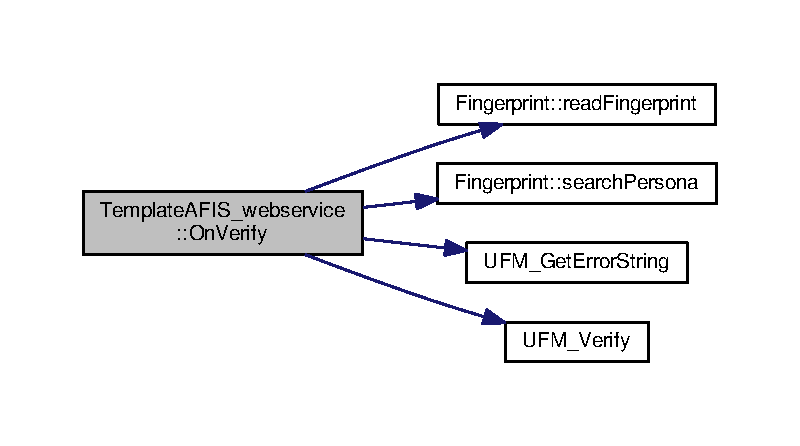
\includegraphics[width=350pt]{classTemplateAFIS__webservice_ad2d94adf36b56bf3306e52e5e20ecaab_cgraph}
\end{center}
\end{figure}
\hypertarget{classTemplateAFIS__webservice_a85f73ddfc479ea1f9ba3a6467d1c028b}{}\label{classTemplateAFIS__webservice_a85f73ddfc479ea1f9ba3a6467d1c028b} 
\index{Template\+A\+F\+I\+S\+\_\+webservice@{Template\+A\+F\+I\+S\+\_\+webservice}!p\+El\+Mismo@{p\+El\+Mismo}}
\index{p\+El\+Mismo@{p\+El\+Mismo}!Template\+A\+F\+I\+S\+\_\+webservice@{Template\+A\+F\+I\+S\+\_\+webservice}}
\subsubsection{\texorpdfstring{p\+El\+Mismo()}{pElMismo()}}
{\footnotesize\ttfamily void $\ast$ Template\+A\+F\+I\+S\+\_\+webservice\+::p\+El\+Mismo (\begin{DoxyParamCaption}{ }\end{DoxyParamCaption})}



p\+El\+Mismo 

\begin{DoxyReturn}{Devuelve}
Obtiene a si mismo.
\end{DoxyReturn}
Obtener el mismo objeto, a sí mismo. 

Definición en la línea 173 del archivo Template\+A\+F\+I\+S.\+cpp.

\hypertarget{classTemplateAFIS__webservice_ae94ac0d97d82afb530698db6f22c0a71}{}\label{classTemplateAFIS__webservice_ae94ac0d97d82afb530698db6f22c0a71} 
\index{Template\+A\+F\+I\+S\+\_\+webservice@{Template\+A\+F\+I\+S\+\_\+webservice}!private\+\_\+decrypt@{private\+\_\+decrypt}}
\index{private\+\_\+decrypt@{private\+\_\+decrypt}!Template\+A\+F\+I\+S\+\_\+webservice@{Template\+A\+F\+I\+S\+\_\+webservice}}
\subsubsection{\texorpdfstring{private\+\_\+decrypt()}{private\_decrypt()}}
{\footnotesize\ttfamily int Template\+A\+F\+I\+S\+\_\+webservice\+::private\+\_\+decrypt (\begin{DoxyParamCaption}\item[{unsigned char $\ast$}]{enc\+\_\+data,  }\item[{int}]{data\+\_\+len,  }\item[{unsigned char $\ast$}]{key,  }\item[{unsigned char $\ast$}]{decrypted }\end{DoxyParamCaption})}



private\+\_\+decrypt 


\begin{DoxyParams}{Parámetros}
{\em enc\+\_\+data} & Data encriptada \\
\hline
{\em data\+\_\+len} & Tamaño de data encriptada \\
\hline
{\em key} & Llave privada \\
\hline
{\em decrypted} & Resultado de la desencriptación \\
\hline
\end{DoxyParams}


Definición en la línea 2496 del archivo Template\+A\+F\+I\+S.\+cpp.

\hypertarget{classTemplateAFIS__webservice_ad332d60ad475ff5ec824d4a004defb45}{}\label{classTemplateAFIS__webservice_ad332d60ad475ff5ec824d4a004defb45} 
\index{Template\+A\+F\+I\+S\+\_\+webservice@{Template\+A\+F\+I\+S\+\_\+webservice}!private\+\_\+encrypt@{private\+\_\+encrypt}}
\index{private\+\_\+encrypt@{private\+\_\+encrypt}!Template\+A\+F\+I\+S\+\_\+webservice@{Template\+A\+F\+I\+S\+\_\+webservice}}
\subsubsection{\texorpdfstring{private\+\_\+encrypt()}{private\_encrypt()}}
{\footnotesize\ttfamily int Template\+A\+F\+I\+S\+\_\+webservice\+::private\+\_\+encrypt (\begin{DoxyParamCaption}\item[{unsigned char $\ast$}]{data,  }\item[{int}]{data\+\_\+len,  }\item[{unsigned char $\ast$}]{key,  }\item[{unsigned char $\ast$}]{encrypted }\end{DoxyParamCaption})}



private\+\_\+encrypt 


\begin{DoxyParams}{Parámetros}
{\em data} & Data a encriptar \\
\hline
{\em data\+\_\+len} & Tamaño de data a encriptar \\
\hline
{\em key} & Llave privada \\
\hline
{\em encrypted} & Resultado de la encriptación \\
\hline
\end{DoxyParams}


Definición en la línea 2504 del archivo Template\+A\+F\+I\+S.\+cpp.

\hypertarget{classTemplateAFIS__webservice_a881bbae5e1b28f4bb6e821f7cae1fdde}{}\label{classTemplateAFIS__webservice_a881bbae5e1b28f4bb6e821f7cae1fdde} 
\index{Template\+A\+F\+I\+S\+\_\+webservice@{Template\+A\+F\+I\+S\+\_\+webservice}!public\+\_\+decrypt@{public\+\_\+decrypt}}
\index{public\+\_\+decrypt@{public\+\_\+decrypt}!Template\+A\+F\+I\+S\+\_\+webservice@{Template\+A\+F\+I\+S\+\_\+webservice}}
\subsubsection{\texorpdfstring{public\+\_\+decrypt()}{public\_decrypt()}}
{\footnotesize\ttfamily int Template\+A\+F\+I\+S\+\_\+webservice\+::public\+\_\+decrypt (\begin{DoxyParamCaption}\item[{unsigned char $\ast$}]{enc\+\_\+data,  }\item[{int}]{data\+\_\+len,  }\item[{unsigned char $\ast$}]{key,  }\item[{unsigned char $\ast$}]{decrypted }\end{DoxyParamCaption})}



public\+\_\+decrypt 


\begin{DoxyParams}{Parámetros}
{\em enc\+\_\+data} & Data encriptada \\
\hline
{\em data\+\_\+len} & Tamaño de data encriptada \\
\hline
{\em key} & Llave pública \\
\hline
{\em decrypted} & Resultado de la desencriptación \\
\hline
\end{DoxyParams}


Definición en la línea 2511 del archivo Template\+A\+F\+I\+S.\+cpp.

\hypertarget{classTemplateAFIS__webservice_ac758d0e51ad6676b2bd2659d4438ae35}{}\label{classTemplateAFIS__webservice_ac758d0e51ad6676b2bd2659d4438ae35} 
\index{Template\+A\+F\+I\+S\+\_\+webservice@{Template\+A\+F\+I\+S\+\_\+webservice}!public\+\_\+encrypt@{public\+\_\+encrypt}}
\index{public\+\_\+encrypt@{public\+\_\+encrypt}!Template\+A\+F\+I\+S\+\_\+webservice@{Template\+A\+F\+I\+S\+\_\+webservice}}
\subsubsection{\texorpdfstring{public\+\_\+encrypt()}{public\_encrypt()}}
{\footnotesize\ttfamily int Template\+A\+F\+I\+S\+\_\+webservice\+::public\+\_\+encrypt (\begin{DoxyParamCaption}\item[{unsigned char $\ast$}]{data,  }\item[{int}]{data\+\_\+len,  }\item[{unsigned char $\ast$}]{key,  }\item[{unsigned char $\ast$}]{encrypted }\end{DoxyParamCaption})}



public\+\_\+encrypt 


\begin{DoxyParams}{Parámetros}
{\em data} & Data a encriptar \\
\hline
{\em data\+\_\+len} & Tamaño de data a encriptar \\
\hline
{\em key} & Llave pública \\
\hline
{\em encrypted} & Resultado de la encriptación \\
\hline
\end{DoxyParams}


Definición en la línea 2489 del archivo Template\+A\+F\+I\+S.\+cpp.

\hypertarget{classTemplateAFIS__webservice_a8e3f9279cbfd23a0a89d62c19ddd007c}{}\label{classTemplateAFIS__webservice_a8e3f9279cbfd23a0a89d62c19ddd007c} 
\index{Template\+A\+F\+I\+S\+\_\+webservice@{Template\+A\+F\+I\+S\+\_\+webservice}!salvar\+J\+P\+EG@{salvar\+J\+P\+EG}}
\index{salvar\+J\+P\+EG@{salvar\+J\+P\+EG}!Template\+A\+F\+I\+S\+\_\+webservice@{Template\+A\+F\+I\+S\+\_\+webservice}}
\subsubsection{\texorpdfstring{salvar\+J\+P\+E\+G()}{salvarJPEG()}}
{\footnotesize\ttfamily int Template\+A\+F\+I\+S\+\_\+webservice\+::salvar\+J\+P\+EG (\begin{DoxyParamCaption}\item[{string}]{usuario,  }\item[{string}]{password,  }\item[{string}]{id\+\_\+persona,  }\item[{string}]{id\+\_\+dedo,  }\item[{string}]{mano,  }\item[{unsigned char $\ast$\&}]{imagen\+\_\+buffer,  }\item[{int \&}]{width,  }\item[{int \&}]{height,  }\item[{int \&}]{size,  }\item[{string \&}]{id\+\_\+imagen }\end{DoxyParamCaption})}



Salvar J\+P\+EG\+: Salva una imágen a J\+P\+EG. 


\begin{DoxyParams}{Parámetros}
{\em usuario} & Usuario U\+RE \\
\hline
{\em password} & Password U\+RE \\
\hline
{\em id\+\_\+persona} & Cédula de la persona \\
\hline
{\em id\+\_\+dedo} & Dedo de la persona \\
\hline
{\em mano} & Mano de la persona \\
\hline
{\em imagen\+\_\+buffer} & Buffer donde se guardará la imágen \\
\hline
{\em width} & Ancho de Imágen \\
\hline
{\em height} & Alto de Imágen \\
\hline
{\em size} & Tamaño de Imágen \\
\hline
{\em id\+\_\+imagen} & Id de la Imágen \\
\hline
\end{DoxyParams}
\begin{DoxyReturn}{Devuelve}
Estado.
\end{DoxyReturn}
Método salvar\+J\+P\+EG\+: Extrae una imágen de la Base de Datos. Almacena las imagenes jpg de las huellas en la Base de datos de Odoo. Verifica el usuario que realiza la petición y sus permisos, luego busca la huella en la base de datos del usuario. Si la encuentra, la convierte y la almacena en imagen\+\_\+buffer. 

Definición en la línea 1417 del archivo Template\+A\+F\+I\+S.\+cpp.



Hace referencia a Imagen\+::id, N\+A\+ME, Imagen\+::n\+Height, Imagen\+::n\+Size, Imagen\+::n\+Width, Fingerprint\+::read\+Fingerprint\+Image(), Fingerprint\+::search\+Persona(), Fingerprint\+::\+U\+RL y V\+E\+R\+S\+I\+ON.

Gráfico de llamadas para esta función\+:\nopagebreak
\begin{figure}[H]
\begin{center}
\leavevmode
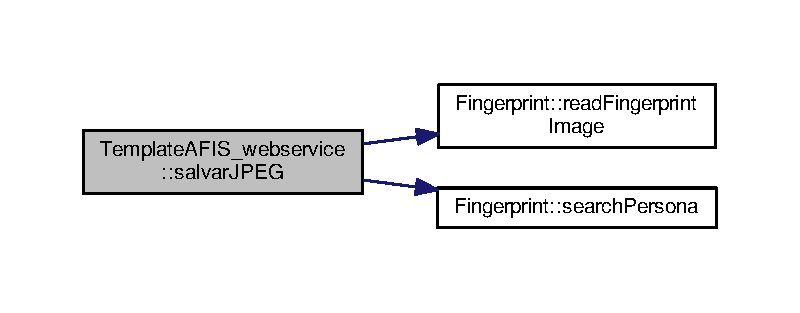
\includegraphics[width=350pt]{classTemplateAFIS__webservice_a8e3f9279cbfd23a0a89d62c19ddd007c_cgraph}
\end{center}
\end{figure}
\hypertarget{classTemplateAFIS__webservice_ae233b5bd61f6754d877e54788332fe92}{}\label{classTemplateAFIS__webservice_ae233b5bd61f6754d877e54788332fe92} 
\index{Template\+A\+F\+I\+S\+\_\+webservice@{Template\+A\+F\+I\+S\+\_\+webservice}!Save\+Imagen\+W\+SQ@{Save\+Imagen\+W\+SQ}}
\index{Save\+Imagen\+W\+SQ@{Save\+Imagen\+W\+SQ}!Template\+A\+F\+I\+S\+\_\+webservice@{Template\+A\+F\+I\+S\+\_\+webservice}}
\subsubsection{\texorpdfstring{Save\+Imagen\+W\+S\+Q()}{SaveImagenWSQ()}}
{\footnotesize\ttfamily void Template\+A\+F\+I\+S\+\_\+webservice\+::\+Save\+Imagen\+W\+SQ (\begin{DoxyParamCaption}{ }\end{DoxyParamCaption})}



Save Imagen\+W\+SQ\+: Salva el Template a W\+SQ. (En pruebas) 



Definición en la línea 183 del archivo Template\+A\+F\+I\+S.\+cpp.

\hypertarget{classTemplateAFIS__webservice_afc08ffa4abcde0b3c0f1c13d973755e1}{}\label{classTemplateAFIS__webservice_afc08ffa4abcde0b3c0f1c13d973755e1} 
\index{Template\+A\+F\+I\+S\+\_\+webservice@{Template\+A\+F\+I\+S\+\_\+webservice}!Save\+Template2\+I\+SO@{Save\+Template2\+I\+SO}}
\index{Save\+Template2\+I\+SO@{Save\+Template2\+I\+SO}!Template\+A\+F\+I\+S\+\_\+webservice@{Template\+A\+F\+I\+S\+\_\+webservice}}
\subsubsection{\texorpdfstring{Save\+Template2\+I\+S\+O()}{SaveTemplate2ISO()}}
{\footnotesize\ttfamily void Template\+A\+F\+I\+S\+\_\+webservice\+::\+Save\+Template2\+I\+SO (\begin{DoxyParamCaption}{ }\end{DoxyParamCaption})}



Save Template2\+I\+SO\+: Salva el Template a I\+SO. (En pruebas) 



Definición en la línea 182 del archivo Template\+A\+F\+I\+S.\+cpp.

\hypertarget{classTemplateAFIS__webservice_a6357de3d3323010cb5890d2f583e0f94}{}\label{classTemplateAFIS__webservice_a6357de3d3323010cb5890d2f583e0f94} 
\index{Template\+A\+F\+I\+S\+\_\+webservice@{Template\+A\+F\+I\+S\+\_\+webservice}!Set\+Tipo\+Template@{Set\+Tipo\+Template}}
\index{Set\+Tipo\+Template@{Set\+Tipo\+Template}!Template\+A\+F\+I\+S\+\_\+webservice@{Template\+A\+F\+I\+S\+\_\+webservice}}
\subsubsection{\texorpdfstring{Set\+Tipo\+Template()}{SetTipoTemplate()}}
{\footnotesize\ttfamily void Template\+A\+F\+I\+S\+\_\+webservice\+::\+Set\+Tipo\+Template (\begin{DoxyParamCaption}\item[{int}]{tipo }\end{DoxyParamCaption})}



Set Tipo Template. 


\begin{DoxyParams}{Parámetros}
{\em tipo} & Tipo de template\\
\hline
\end{DoxyParams}
Método Set\+Tipo\+Template\+: Establece el tipo de Template. 

Definición en la línea 181 del archivo Template\+A\+F\+I\+S.\+cpp.

\hypertarget{classTemplateAFIS__webservice_a90522f2c2f10ae8fa3ab6abd0273b714}{}\label{classTemplateAFIS__webservice_a90522f2c2f10ae8fa3ab6abd0273b714} 
\index{Template\+A\+F\+I\+S\+\_\+webservice@{Template\+A\+F\+I\+S\+\_\+webservice}!un\+Init\+Matcher@{un\+Init\+Matcher}}
\index{un\+Init\+Matcher@{un\+Init\+Matcher}!Template\+A\+F\+I\+S\+\_\+webservice@{Template\+A\+F\+I\+S\+\_\+webservice}}
\subsubsection{\texorpdfstring{un\+Init\+Matcher()}{unInitMatcher()}}
{\footnotesize\ttfamily bool Template\+A\+F\+I\+S\+\_\+webservice\+::un\+Init\+Matcher (\begin{DoxyParamCaption}{ }\end{DoxyParamCaption})}



un\+Init Matcher 

\begin{DoxyReturn}{Devuelve}
Obtiene el estado de desinicialización del Matcher. True o False
\end{DoxyReturn}
Método un\+Init\+Matcher\+: Desinicializa el Matcher. Protocolo de S\+U\+P\+R\+E\+MA indicado en el S\+DK 

Definición en la línea 258 del archivo Template\+A\+F\+I\+S.\+cpp.



Hace referencia a U\+F\+M\+\_\+\+Delete(), U\+F\+M\+\_\+\+OK y U\+F\+M\+\_\+\+S\+T\+A\+T\+US.

Gráfico de llamadas para esta función\+:\nopagebreak
\begin{figure}[H]
\begin{center}
\leavevmode
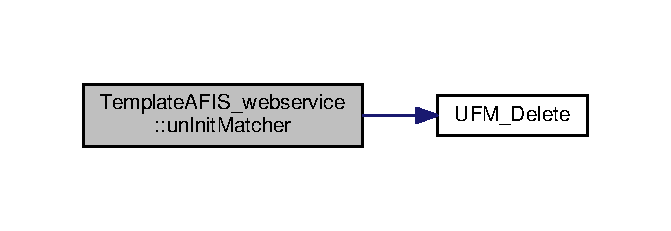
\includegraphics[width=322pt]{classTemplateAFIS__webservice_a90522f2c2f10ae8fa3ab6abd0273b714_cgraph}
\end{center}
\end{figure}


\subsection{Documentación de los datos miembro}
\hypertarget{classTemplateAFIS__webservice_a09c632296df4dd488ab09fee6e26f4eb}{}\label{classTemplateAFIS__webservice_a09c632296df4dd488ab09fee6e26f4eb} 
\index{Template\+A\+F\+I\+S\+\_\+webservice@{Template\+A\+F\+I\+S\+\_\+webservice}!base64\+\_\+chars@{base64\+\_\+chars}}
\index{base64\+\_\+chars@{base64\+\_\+chars}!Template\+A\+F\+I\+S\+\_\+webservice@{Template\+A\+F\+I\+S\+\_\+webservice}}
\subsubsection{\texorpdfstring{base64\+\_\+chars}{base64\_chars}}
{\footnotesize\ttfamily std\+::string Template\+A\+F\+I\+S\+\_\+webservice\+::base64\+\_\+chars\hspace{0.3cm}{\ttfamily [private]}}



base64\+\_\+chars 



Definición en la línea 238 del archivo Template\+A\+F\+I\+S.\+h.

\hypertarget{classTemplateAFIS__webservice_a829e57a86d8c1c0b17631eebf8a8e0cf}{}\label{classTemplateAFIS__webservice_a829e57a86d8c1c0b17631eebf8a8e0cf} 
\index{Template\+A\+F\+I\+S\+\_\+webservice@{Template\+A\+F\+I\+S\+\_\+webservice}!firma\+\_\+digital@{firma\+\_\+digital}}
\index{firma\+\_\+digital@{firma\+\_\+digital}!Template\+A\+F\+I\+S\+\_\+webservice@{Template\+A\+F\+I\+S\+\_\+webservice}}
\subsubsection{\texorpdfstring{firma\+\_\+digital}{firma\_digital}}
{\footnotesize\ttfamily \hyperlink{classFirmaDigital}{Firma\+Digital}$\ast$ Template\+A\+F\+I\+S\+\_\+webservice\+::firma\+\_\+digital}



firma\+\_\+figital 



Definición en la línea 260 del archivo Template\+A\+F\+I\+S.\+h.

\hypertarget{classTemplateAFIS__webservice_a2c8421c26cc3dd7d6a3295ace4fd82ce}{}\label{classTemplateAFIS__webservice_a2c8421c26cc3dd7d6a3295ace4fd82ce} 
\index{Template\+A\+F\+I\+S\+\_\+webservice@{Template\+A\+F\+I\+S\+\_\+webservice}!m\+\_\+b\+Fast\+Mode@{m\+\_\+b\+Fast\+Mode}}
\index{m\+\_\+b\+Fast\+Mode@{m\+\_\+b\+Fast\+Mode}!Template\+A\+F\+I\+S\+\_\+webservice@{Template\+A\+F\+I\+S\+\_\+webservice}}
\subsubsection{\texorpdfstring{m\+\_\+b\+Fast\+Mode}{m\_bFastMode}}
{\footnotesize\ttfamily bool Template\+A\+F\+I\+S\+\_\+webservice\+::m\+\_\+b\+Fast\+Mode\hspace{0.3cm}{\ttfamily [private]}}



m\+\_\+b\+Fast\+Mode 



Definición en la línea 221 del archivo Template\+A\+F\+I\+S.\+h.

\hypertarget{classTemplateAFIS__webservice_a9e97e8c2a5aa5de8ee51fbdfe4644c39}{}\label{classTemplateAFIS__webservice_a9e97e8c2a5aa5de8ee51fbdfe4644c39} 
\index{Template\+A\+F\+I\+S\+\_\+webservice@{Template\+A\+F\+I\+S\+\_\+webservice}!m\+\_\+h\+Matcher@{m\+\_\+h\+Matcher}}
\index{m\+\_\+h\+Matcher@{m\+\_\+h\+Matcher}!Template\+A\+F\+I\+S\+\_\+webservice@{Template\+A\+F\+I\+S\+\_\+webservice}}
\subsubsection{\texorpdfstring{m\+\_\+h\+Matcher}{m\_hMatcher}}
{\footnotesize\ttfamily \hyperlink{UFMatcher_8h_a2a955bd8ef5ebcf92278a2b037f6e739}{H\+U\+F\+Matcher} Template\+A\+F\+I\+S\+\_\+webservice\+::m\+\_\+h\+Matcher\hspace{0.3cm}{\ttfamily [private]}}



m\+\_\+h\+Matcher 



Definición en la línea 209 del archivo Template\+A\+F\+I\+S.\+h.

\hypertarget{classTemplateAFIS__webservice_a0d609b06768f2c253f43654966bd41e1}{}\label{classTemplateAFIS__webservice_a0d609b06768f2c253f43654966bd41e1} 
\index{Template\+A\+F\+I\+S\+\_\+webservice@{Template\+A\+F\+I\+S\+\_\+webservice}!m\+\_\+n\+Cur\+Scanner\+Index@{m\+\_\+n\+Cur\+Scanner\+Index}}
\index{m\+\_\+n\+Cur\+Scanner\+Index@{m\+\_\+n\+Cur\+Scanner\+Index}!Template\+A\+F\+I\+S\+\_\+webservice@{Template\+A\+F\+I\+S\+\_\+webservice}}
\subsubsection{\texorpdfstring{m\+\_\+n\+Cur\+Scanner\+Index}{m\_nCurScannerIndex}}
{\footnotesize\ttfamily int Template\+A\+F\+I\+S\+\_\+webservice\+::m\+\_\+n\+Cur\+Scanner\+Index\hspace{0.3cm}{\ttfamily [private]}}



m\+\_\+n\+Cur\+Scanner\+Index 



Definición en la línea 233 del archivo Template\+A\+F\+I\+S.\+h.

\hypertarget{classTemplateAFIS__webservice_ad979fde0c45dd460249d041a669a9914}{}\label{classTemplateAFIS__webservice_ad979fde0c45dd460249d041a669a9914} 
\index{Template\+A\+F\+I\+S\+\_\+webservice@{Template\+A\+F\+I\+S\+\_\+webservice}!m\+\_\+n\+Enroll\+Quality@{m\+\_\+n\+Enroll\+Quality}}
\index{m\+\_\+n\+Enroll\+Quality@{m\+\_\+n\+Enroll\+Quality}!Template\+A\+F\+I\+S\+\_\+webservice@{Template\+A\+F\+I\+S\+\_\+webservice}}
\subsubsection{\texorpdfstring{m\+\_\+n\+Enroll\+Quality}{m\_nEnrollQuality}}
{\footnotesize\ttfamily int Template\+A\+F\+I\+S\+\_\+webservice\+::m\+\_\+n\+Enroll\+Quality\hspace{0.3cm}{\ttfamily [private]}}



m\+\_\+n\+Enroll\+Quality 



Definición en la línea 229 del archivo Template\+A\+F\+I\+S.\+h.

\hypertarget{classTemplateAFIS__webservice_a8809dc8920da337f97252597ef492671}{}\label{classTemplateAFIS__webservice_a8809dc8920da337f97252597ef492671} 
\index{Template\+A\+F\+I\+S\+\_\+webservice@{Template\+A\+F\+I\+S\+\_\+webservice}!m\+\_\+n\+Security\+Level@{m\+\_\+n\+Security\+Level}}
\index{m\+\_\+n\+Security\+Level@{m\+\_\+n\+Security\+Level}!Template\+A\+F\+I\+S\+\_\+webservice@{Template\+A\+F\+I\+S\+\_\+webservice}}
\subsubsection{\texorpdfstring{m\+\_\+n\+Security\+Level}{m\_nSecurityLevel}}
{\footnotesize\ttfamily int Template\+A\+F\+I\+S\+\_\+webservice\+::m\+\_\+n\+Security\+Level\hspace{0.3cm}{\ttfamily [private]}}



m\+\_\+n\+Security\+Level 



Definición en la línea 217 del archivo Template\+A\+F\+I\+S.\+h.

\hypertarget{classTemplateAFIS__webservice_a83ff03441c588729601736d18eb65afd}{}\label{classTemplateAFIS__webservice_a83ff03441c588729601736d18eb65afd} 
\index{Template\+A\+F\+I\+S\+\_\+webservice@{Template\+A\+F\+I\+S\+\_\+webservice}!m\+\_\+str\+Error@{m\+\_\+str\+Error}}
\index{m\+\_\+str\+Error@{m\+\_\+str\+Error}!Template\+A\+F\+I\+S\+\_\+webservice@{Template\+A\+F\+I\+S\+\_\+webservice}}
\subsubsection{\texorpdfstring{m\+\_\+str\+Error}{m\_strError}}
{\footnotesize\ttfamily char Template\+A\+F\+I\+S\+\_\+webservice\+::m\+\_\+str\+Error\mbox{[}128\mbox{]}\hspace{0.3cm}{\ttfamily [private]}}



m\+\_\+str\+Error\mbox{[}128\mbox{]} 



Definición en la línea 225 del archivo Template\+A\+F\+I\+S.\+h.

\hypertarget{classTemplateAFIS__webservice_a5be66b367a1276c21ffc3450c1f69643}{}\label{classTemplateAFIS__webservice_a5be66b367a1276c21ffc3450c1f69643} 
\index{Template\+A\+F\+I\+S\+\_\+webservice@{Template\+A\+F\+I\+S\+\_\+webservice}!padding@{padding}}
\index{padding@{padding}!Template\+A\+F\+I\+S\+\_\+webservice@{Template\+A\+F\+I\+S\+\_\+webservice}}
\subsubsection{\texorpdfstring{padding}{padding}}
{\footnotesize\ttfamily int Template\+A\+F\+I\+S\+\_\+webservice\+::padding\hspace{0.3cm}{\ttfamily [private]}}



padding 



Definición en la línea 243 del archivo Template\+A\+F\+I\+S.\+h.

\hypertarget{classTemplateAFIS__webservice_a955d31aac4c820b4399ccbafe1b59b63}{}\label{classTemplateAFIS__webservice_a955d31aac4c820b4399ccbafe1b59b63} 
\index{Template\+A\+F\+I\+S\+\_\+webservice@{Template\+A\+F\+I\+S\+\_\+webservice}!tipo\+\_\+template@{tipo\+\_\+template}}
\index{tipo\+\_\+template@{tipo\+\_\+template}!Template\+A\+F\+I\+S\+\_\+webservice@{Template\+A\+F\+I\+S\+\_\+webservice}}
\subsubsection{\texorpdfstring{tipo\+\_\+template}{tipo\_template}}
{\footnotesize\ttfamily int Template\+A\+F\+I\+S\+\_\+webservice\+::tipo\+\_\+template\hspace{0.3cm}{\ttfamily [private]}}



tipo\+\_\+template 



Definición en la línea 213 del archivo Template\+A\+F\+I\+S.\+h.



La documentación para esta clase fue generada a partir de los siguientes ficheros\+:\begin{DoxyCompactItemize}
\item 
Template\+A\+F\+I\+S\+\_\+webservice\+\_\+lib/include/\hyperlink{TemplateAFIS_8h}{Template\+A\+F\+I\+S.\+h}\item 
Template\+A\+F\+I\+S\+\_\+webservice\+\_\+lib/include/\hyperlink{TemplateAFIS_8cpp}{Template\+A\+F\+I\+S.\+cpp}\end{DoxyCompactItemize}

\chapter{Documentación de archivos}
\hypertarget{compilar_8sh}{}\section{Referencia del Archivo compilar.\+sh}
\label{compilar_8sh}\index{compilar.\+sh@{compilar.\+sh}}

\hypertarget{instalar_8sh}{}\section{Referencia del Archivo instalar.\+sh}
\label{instalar_8sh}\index{instalar.\+sh@{instalar.\+sh}}

\hypertarget{mainPage_8h}{}\section{Referencia del Archivo main\+Page.\+h}
\label{mainPage_8h}\index{main\+Page.\+h@{main\+Page.\+h}}

\hypertarget{Fingerprint_8cpp}{}\section{Referencia del Archivo Template\+A\+F\+I\+S\+\_\+webservice\+\_\+lib/\+Conexion\+\_\+webservice/\+Fingerprint.cpp}
\label{Fingerprint_8cpp}\index{Template\+A\+F\+I\+S\+\_\+webservice\+\_\+lib/\+Conexion\+\_\+webservice/\+Fingerprint.\+cpp@{Template\+A\+F\+I\+S\+\_\+webservice\+\_\+lib/\+Conexion\+\_\+webservice/\+Fingerprint.\+cpp}}


Clase que permite realizar la interacción con el Webservice con Open\+E\+RP.  


{\ttfamily \#include $<$stdio.\+h$>$}\newline
{\ttfamily \#include $<$string.\+h$>$}\newline
{\ttfamily \#include $<$cstdlib$>$}\newline
{\ttfamily \#include $<$iostream$>$}\newline
{\ttfamily \#include $<$Xml\+Rpc\+Cpp.\+h$>$}\newline
{\ttfamily \#include $<$stdlib.\+h$>$}\newline
{\ttfamily \#include $<$sstream$>$}\newline
{\ttfamily \#include $<$ctime$>$}\newline
{\ttfamily \#include $<$fstream$>$}\newline
{\ttfamily \#include $<$algorithm$>$}\newline
{\ttfamily \#include $<$cctype$>$}\newline
{\ttfamily \#include $<$openssl/sha.\+h$>$}\newline
{\ttfamily \#include $<$openssl/hmac.\+h$>$}\newline
{\ttfamily \#include $<$openssl/evp.\+h$>$}\newline
{\ttfamily \#include $<$openssl/bio.\+h$>$}\newline
{\ttfamily \#include $<$openssl/buffer.\+h$>$}\newline
{\ttfamily \#include $<$openssl/md5.\+h$>$}\newline
Dependencia gráfica adjunta para Fingerprint.\+cpp\+:\nopagebreak
\begin{figure}[H]
\begin{center}
\leavevmode
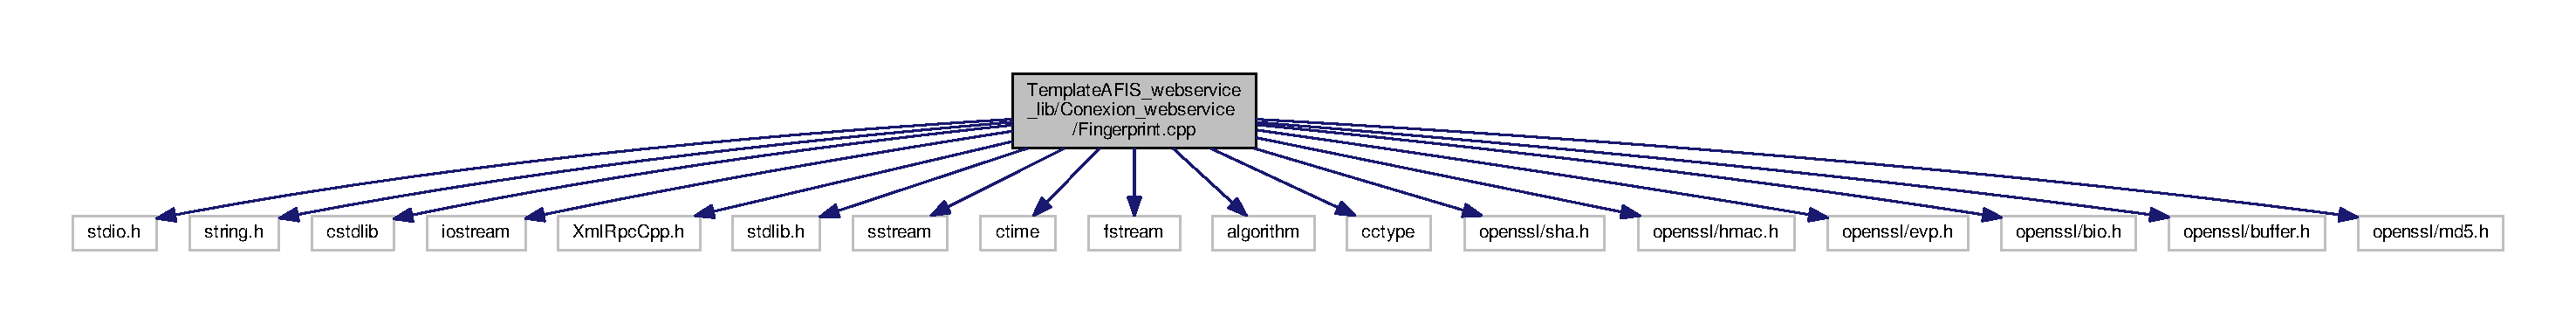
\includegraphics[width=350pt]{Fingerprint_8cpp__incl}
\end{center}
\end{figure}
Gráfico de los archivos que directa o indirectamente incluyen a este archivo\+:\nopagebreak
\begin{figure}[H]
\begin{center}
\leavevmode
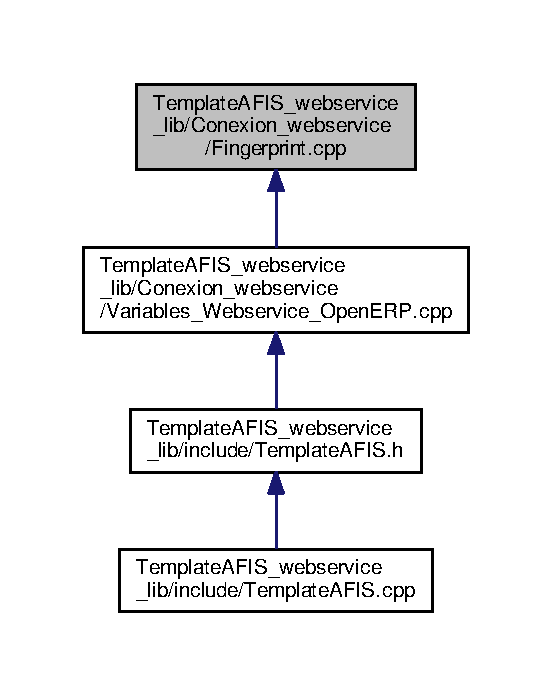
\includegraphics[width=265pt]{Fingerprint_8cpp__dep__incl}
\end{center}
\end{figure}
\subsection*{Clases}
\begin{DoxyCompactItemize}
\item 
class \hyperlink{classFingerprint}{Fingerprint}
\begin{DoxyCompactList}\small\item\em Clase que permite realizar la interacción con el Webservice con Open\+E\+RP. \end{DoxyCompactList}\end{DoxyCompactItemize}
\subsection*{\textquotesingle{}defines\textquotesingle{}}
\begin{DoxyCompactItemize}
\item 
\#define \hyperlink{Fingerprint_8cpp_a47f2e62c0dbebc787052c165afcada0e}{N\+A\+ME}~\char`\"{}X\+ML-\/R\+PC C\+FG C++ Client\char`\"{}
\item 
\#define \hyperlink{Fingerprint_8cpp_a1c6d5de492ac61ad29aec7aa9a436bbf}{V\+E\+R\+S\+I\+ON}~\char`\"{}0.\+1\char`\"{}
\end{DoxyCompactItemize}


\subsection{Descripción detallada}
Clase que permite realizar la interacción con el Webservice con Open\+E\+RP. 

\begin{DoxyAuthor}{Autor}
Asociación Cooperativa Simón Rodríguez para el Conocimiento Libre. \href{mailto:contacto@simonrodriguez.org.ve}{\tt contacto@simonrodriguez.\+org.\+ve} 
\end{DoxyAuthor}
\begin{DoxyAuthor}{Autores}
Lcdo. César Cordero, Ing. Servio Zambrano y Ángel Ramírez Isea. 
\end{DoxyAuthor}
\begin{DoxyDate}{Fecha}
2014 This file is part of Sistema de Identificación Biométrica para las O\+B\+PP. 
\end{DoxyDate}


\subsection{Documentación de los \textquotesingle{}defines\textquotesingle{}}
\hypertarget{Fingerprint_8cpp_a47f2e62c0dbebc787052c165afcada0e}{}\label{Fingerprint_8cpp_a47f2e62c0dbebc787052c165afcada0e} 
\index{Fingerprint.\+cpp@{Fingerprint.\+cpp}!N\+A\+ME@{N\+A\+ME}}
\index{N\+A\+ME@{N\+A\+ME}!Fingerprint.\+cpp@{Fingerprint.\+cpp}}
\subsubsection{\texorpdfstring{N\+A\+ME}{NAME}}
{\footnotesize\ttfamily \#define N\+A\+ME~\char`\"{}X\+ML-\/R\+PC C\+FG C++ Client\char`\"{}}



Definición en la línea 13 del archivo Fingerprint.\+cpp.



Referenciado por Template\+A\+F\+I\+S\+\_\+webservice\+::borrar\+Huella(), Template\+A\+F\+I\+S\+\_\+webservice\+::get\+Datos\+Huella(), Template\+A\+F\+I\+S\+\_\+webservice\+::get\+Datos\+Id\+Imagen(), Template\+A\+F\+I\+S\+\_\+webservice\+::get\+Datos\+Persona(), Template\+A\+F\+I\+S\+\_\+webservice\+::get\+Datos\+Persona\+O\+B\+P\+P(), Template\+A\+F\+I\+S\+\_\+webservice\+::get\+Datos\+Persona\+Verificacion(), Template\+A\+F\+I\+S\+\_\+webservice\+::get\+Usuario(), Template\+A\+F\+I\+S\+\_\+webservice\+::\+On\+Enroll(), Template\+A\+F\+I\+S\+\_\+webservice\+::\+On\+Identify(), Template\+A\+F\+I\+S\+\_\+webservice\+::\+On\+Identify\+On\+Verify(), Template\+A\+F\+I\+S\+\_\+webservice\+::\+On\+Verify() y Template\+A\+F\+I\+S\+\_\+webservice\+::salvar\+J\+P\+E\+G().

\hypertarget{Fingerprint_8cpp_a1c6d5de492ac61ad29aec7aa9a436bbf}{}\label{Fingerprint_8cpp_a1c6d5de492ac61ad29aec7aa9a436bbf} 
\index{Fingerprint.\+cpp@{Fingerprint.\+cpp}!V\+E\+R\+S\+I\+ON@{V\+E\+R\+S\+I\+ON}}
\index{V\+E\+R\+S\+I\+ON@{V\+E\+R\+S\+I\+ON}!Fingerprint.\+cpp@{Fingerprint.\+cpp}}
\subsubsection{\texorpdfstring{V\+E\+R\+S\+I\+ON}{VERSION}}
{\footnotesize\ttfamily \#define V\+E\+R\+S\+I\+ON~\char`\"{}0.\+1\char`\"{}}



Definición en la línea 17 del archivo Fingerprint.\+cpp.



Referenciado por Template\+A\+F\+I\+S\+\_\+webservice\+::borrar\+Huella(), Template\+A\+F\+I\+S\+\_\+webservice\+::get\+Datos\+Huella(), Template\+A\+F\+I\+S\+\_\+webservice\+::get\+Datos\+Id\+Imagen(), Template\+A\+F\+I\+S\+\_\+webservice\+::get\+Datos\+Persona(), Template\+A\+F\+I\+S\+\_\+webservice\+::get\+Datos\+Persona\+O\+B\+P\+P(), Template\+A\+F\+I\+S\+\_\+webservice\+::get\+Datos\+Persona\+Verificacion(), Template\+A\+F\+I\+S\+\_\+webservice\+::get\+Usuario(), Template\+A\+F\+I\+S\+\_\+webservice\+::\+On\+Enroll(), Template\+A\+F\+I\+S\+\_\+webservice\+::\+On\+Identify(), Template\+A\+F\+I\+S\+\_\+webservice\+::\+On\+Identify\+On\+Verify(), Template\+A\+F\+I\+S\+\_\+webservice\+::\+On\+Verify() y Template\+A\+F\+I\+S\+\_\+webservice\+::salvar\+J\+P\+E\+G().


\hypertarget{GuiWsOpenErp_8cpp}{}\section{Referencia del Archivo Template\+A\+F\+I\+S\+\_\+webservice\+\_\+lib/\+Conexion\+\_\+webservice/\+Gui\+Ws\+Open\+Erp.cpp}
\label{GuiWsOpenErp_8cpp}\index{Template\+A\+F\+I\+S\+\_\+webservice\+\_\+lib/\+Conexion\+\_\+webservice/\+Gui\+Ws\+Open\+Erp.\+cpp@{Template\+A\+F\+I\+S\+\_\+webservice\+\_\+lib/\+Conexion\+\_\+webservice/\+Gui\+Ws\+Open\+Erp.\+cpp}}


Archivo de cabecera de las clases \hyperlink{classGuiWsOpenErp}{Gui\+Ws\+Open\+Erp}.  


{\ttfamily \#include $<$stdio.\+h$>$}\newline
{\ttfamily \#include $<$string.\+h$>$}\newline
{\ttfamily \#include $<$cstdlib$>$}\newline
{\ttfamily \#include $<$iostream$>$}\newline
{\ttfamily \#include $<$Xml\+Rpc\+Cpp.\+h$>$}\newline
{\ttfamily \#include $<$stdlib.\+h$>$}\newline
{\ttfamily \#include $<$sstream$>$}\newline
{\ttfamily \#include $<$ctime$>$}\newline
{\ttfamily \#include $<$fstream$>$}\newline
{\ttfamily \#include $<$algorithm$>$}\newline
{\ttfamily \#include $<$cctype$>$}\newline
Dependencia gráfica adjunta para Gui\+Ws\+Open\+Erp.\+cpp\+:\nopagebreak
\begin{figure}[H]
\begin{center}
\leavevmode
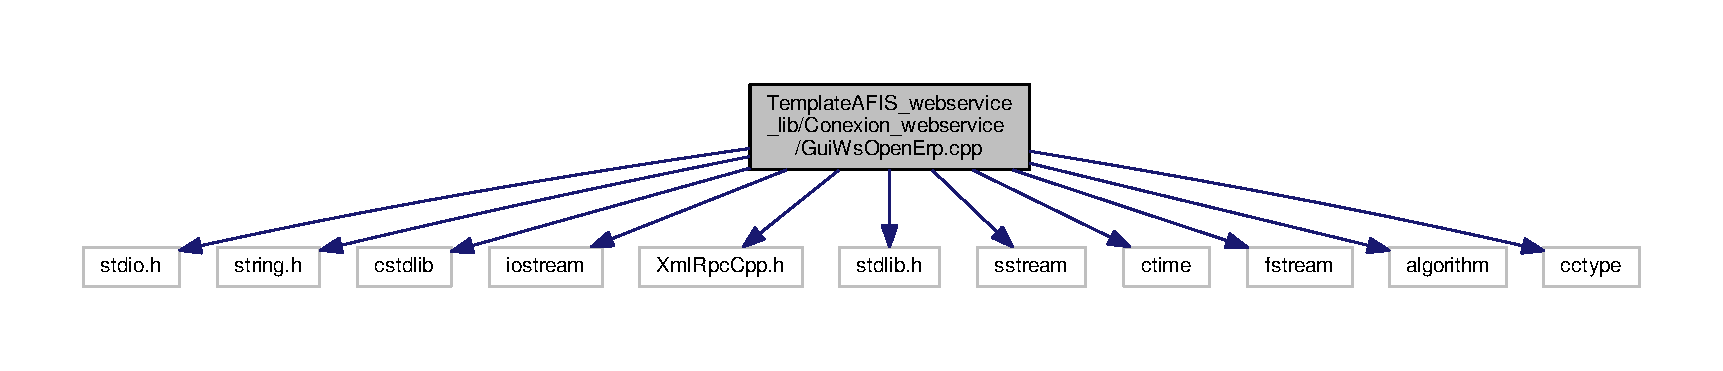
\includegraphics[width=350pt]{GuiWsOpenErp_8cpp__incl}
\end{center}
\end{figure}
Gráfico de los archivos que directa o indirectamente incluyen a este archivo\+:\nopagebreak
\begin{figure}[H]
\begin{center}
\leavevmode
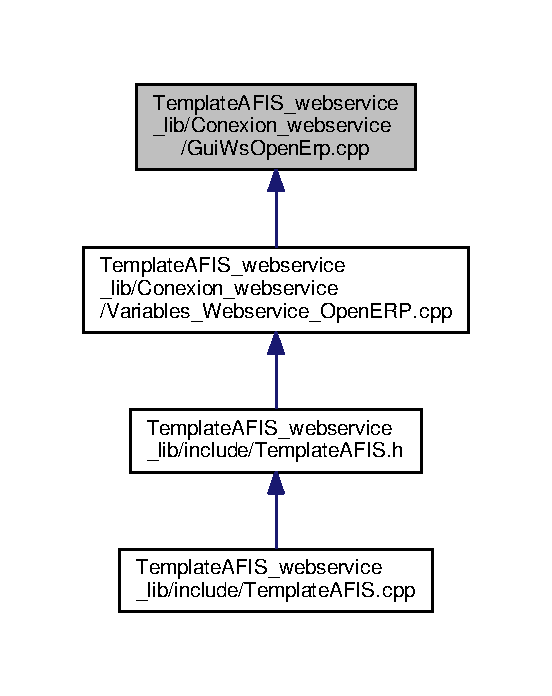
\includegraphics[width=265pt]{GuiWsOpenErp_8cpp__dep__incl}
\end{center}
\end{figure}
\subsection*{Clases}
\begin{DoxyCompactItemize}
\item 
class \hyperlink{classGuiWsOpenErp}{Gui\+Ws\+Open\+Erp}
\begin{DoxyCompactList}\small\item\em Clase que permite realizar la interacción con el Webservice con Open\+E\+RP. (No están en uso actualmente.) \end{DoxyCompactList}\end{DoxyCompactItemize}
\subsection*{\textquotesingle{}defines\textquotesingle{}}
\begin{DoxyCompactItemize}
\item 
\#define \hyperlink{GuiWsOpenErp_8cpp_a47f2e62c0dbebc787052c165afcada0e}{N\+A\+ME}~\char`\"{}X\+ML-\/R\+PC C\+FG C++ Client\char`\"{}
\item 
\#define \hyperlink{GuiWsOpenErp_8cpp_a1c6d5de492ac61ad29aec7aa9a436bbf}{V\+E\+R\+S\+I\+ON}~\char`\"{}0.\+1\char`\"{}
\end{DoxyCompactItemize}


\subsection{Descripción detallada}
Archivo de cabecera de las clases \hyperlink{classGuiWsOpenErp}{Gui\+Ws\+Open\+Erp}. 

\begin{DoxyAuthor}{Autor}
Asociación Cooperativa Simón Rodríguez para el Conocimiento Libre. \href{mailto:contacto@simonrodriguez.org.ve}{\tt contacto@simonrodriguez.\+org.\+ve} 

Lcdo. César Cordero, Ing. Servio Zambrano y Ángel Ramírez Isea. 
\end{DoxyAuthor}
\begin{DoxyDate}{Fecha}
2014 This file is part of Sistema de Identificación Biométrica para las O\+B\+PP. 
\end{DoxyDate}


\subsection{Documentación de los \textquotesingle{}defines\textquotesingle{}}
\hypertarget{GuiWsOpenErp_8cpp_a47f2e62c0dbebc787052c165afcada0e}{}\label{GuiWsOpenErp_8cpp_a47f2e62c0dbebc787052c165afcada0e} 
\index{Gui\+Ws\+Open\+Erp.\+cpp@{Gui\+Ws\+Open\+Erp.\+cpp}!N\+A\+ME@{N\+A\+ME}}
\index{N\+A\+ME@{N\+A\+ME}!Gui\+Ws\+Open\+Erp.\+cpp@{Gui\+Ws\+Open\+Erp.\+cpp}}
\subsubsection{\texorpdfstring{N\+A\+ME}{NAME}}
{\footnotesize\ttfamily \#define N\+A\+ME~\char`\"{}X\+ML-\/R\+PC C\+FG C++ Client\char`\"{}}



Definición en la línea 14 del archivo Gui\+Ws\+Open\+Erp.\+cpp.



Referenciado por Gui\+Ws\+Open\+Erp\+::\+Get\+Persona\+By\+O\+B\+P\+P() y Gui\+Ws\+Open\+Erp\+::\+Inicializar().

\hypertarget{GuiWsOpenErp_8cpp_a1c6d5de492ac61ad29aec7aa9a436bbf}{}\label{GuiWsOpenErp_8cpp_a1c6d5de492ac61ad29aec7aa9a436bbf} 
\index{Gui\+Ws\+Open\+Erp.\+cpp@{Gui\+Ws\+Open\+Erp.\+cpp}!V\+E\+R\+S\+I\+ON@{V\+E\+R\+S\+I\+ON}}
\index{V\+E\+R\+S\+I\+ON@{V\+E\+R\+S\+I\+ON}!Gui\+Ws\+Open\+Erp.\+cpp@{Gui\+Ws\+Open\+Erp.\+cpp}}
\subsubsection{\texorpdfstring{V\+E\+R\+S\+I\+ON}{VERSION}}
{\footnotesize\ttfamily \#define V\+E\+R\+S\+I\+ON~\char`\"{}0.\+1\char`\"{}}



Definición en la línea 19 del archivo Gui\+Ws\+Open\+Erp.\+cpp.



Referenciado por Gui\+Ws\+Open\+Erp\+::\+Get\+Persona\+By\+O\+B\+P\+P() y Gui\+Ws\+Open\+Erp\+::\+Inicializar().


\hypertarget{Variables__Webservice__OpenERP_8cpp}{}\section{Referencia del Archivo Template\+A\+F\+I\+S\+\_\+webservice\+\_\+lib/\+Conexion\+\_\+webservice/\+Variables\+\_\+\+Webservice\+\_\+\+Open\+E\+RP.cpp}
\label{Variables__Webservice__OpenERP_8cpp}\index{Template\+A\+F\+I\+S\+\_\+webservice\+\_\+lib/\+Conexion\+\_\+webservice/\+Variables\+\_\+\+Webservice\+\_\+\+Open\+E\+R\+P.\+cpp@{Template\+A\+F\+I\+S\+\_\+webservice\+\_\+lib/\+Conexion\+\_\+webservice/\+Variables\+\_\+\+Webservice\+\_\+\+Open\+E\+R\+P.\+cpp}}


Archivo de puente entre \hyperlink{classTemplateAFIS__webservice}{Template\+A\+F\+I\+S\+\_\+webservice} y, \hyperlink{classFingerprint}{Fingerprint} y Gui\+Ws\+Open\+E\+RP. Conexión del Webservice con Odoo. Se especifican los parámetros de conexión.  


{\ttfamily \#include \char`\"{}Fingerprint.\+cpp\char`\"{}}\newline
{\ttfamily \#include \char`\"{}Gui\+Ws\+Open\+Erp.\+cpp\char`\"{}}\newline
Dependencia gráfica adjunta para Variables\+\_\+\+Webservice\+\_\+\+Open\+E\+R\+P.\+cpp\+:\nopagebreak
\begin{figure}[H]
\begin{center}
\leavevmode
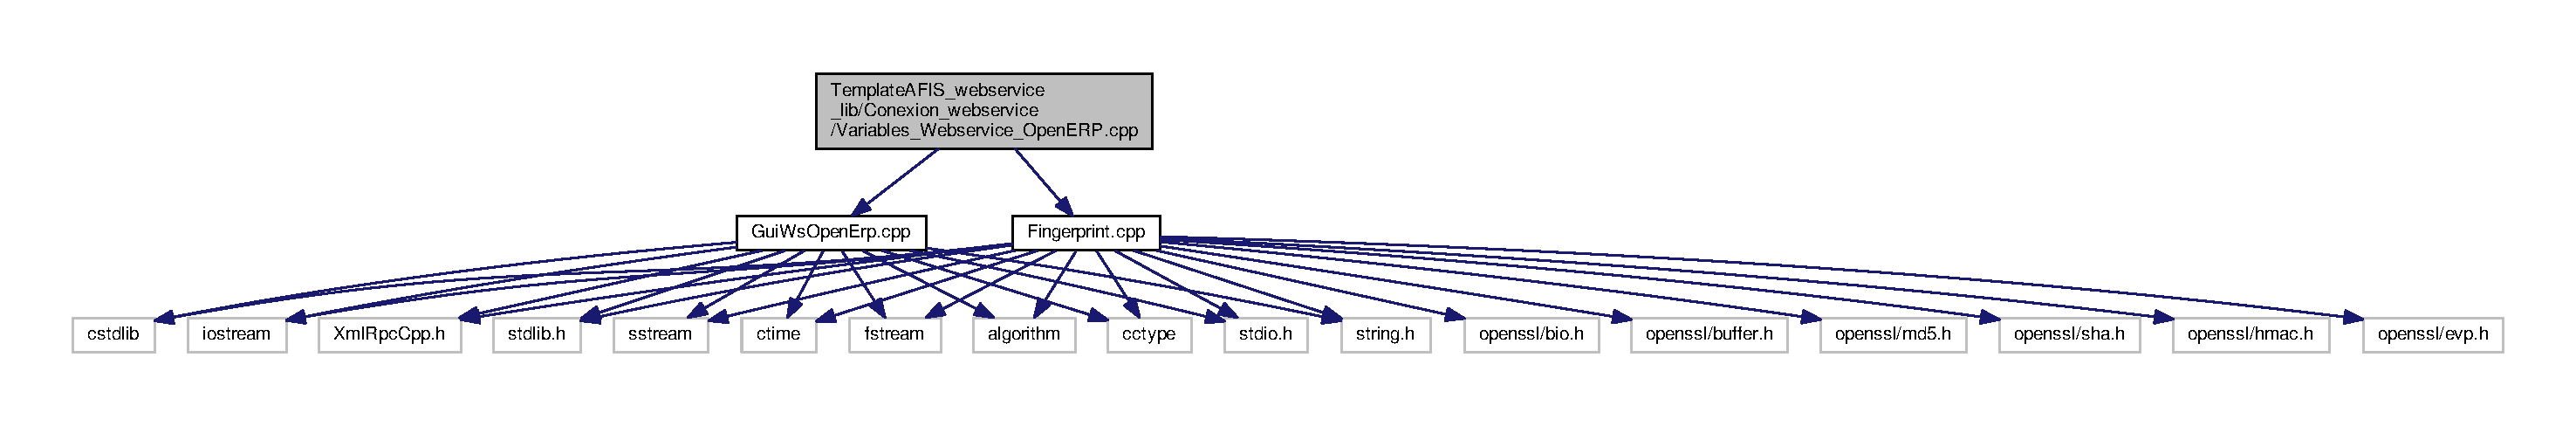
\includegraphics[width=350pt]{Variables__Webservice__OpenERP_8cpp__incl}
\end{center}
\end{figure}
Gráfico de los archivos que directa o indirectamente incluyen a este archivo\+:\nopagebreak
\begin{figure}[H]
\begin{center}
\leavevmode
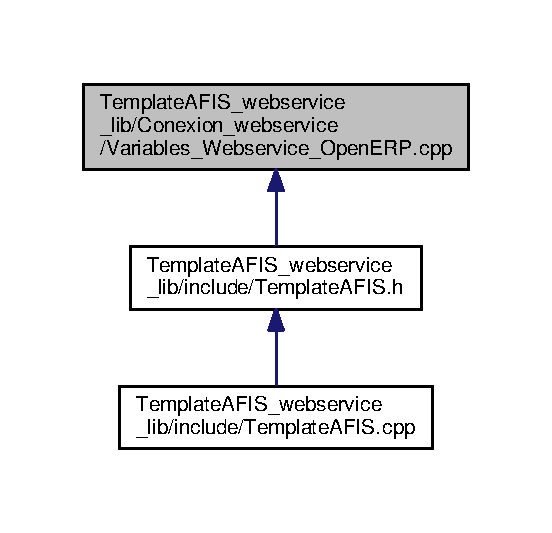
\includegraphics[width=265pt]{Variables__Webservice__OpenERP_8cpp__dep__incl}
\end{center}
\end{figure}
\subsection*{\textquotesingle{}defines\textquotesingle{}}
\begin{DoxyCompactItemize}
\item 
\#define \hyperlink{Variables__Webservice__OpenERP_8cpp_a038affabc8202723068994b56f58d3d6}{W\+E\+B\+S\+E\+R\+V\+I\+C\+ES}~\{ \{\char`\"{}\char`\"{}, \char`\"{}\char`\"{}\}, \{\char`\"{}\char`\"{}, \char`\"{}\char`\"{}\} \};
\begin{DoxyCompactList}\small\item\em Se define la clase principal W\+E\+B\+S\+E\+R\+V\+I\+C\+ES No cambiar estos valores, a menos que modifiquen el código fuente N\+U\+M\+\_\+\+C\+O\+N\+E\+X\+I\+O\+N\+ES debe ser mayor o igual a 2, nunca menor. \end{DoxyCompactList}\item 
\#define \hyperlink{Variables__Webservice__OpenERP_8cpp_a9c1896bf4b60da60fa2ed167f842e81a}{N\+U\+M\+\_\+\+W\+E\+B\+S\+E\+R\+V\+I\+CE}~2
\begin{DoxyCompactList}\small\item\em N\+U\+M\+\_\+\+W\+E\+B\+S\+E\+R\+V\+I\+CE N\+U\+M\+\_\+\+P\+A\+R\+A\+MS debe ser siempre igual a 5. \end{DoxyCompactList}\item 
\#define \hyperlink{Variables__Webservice__OpenERP_8cpp_adb8e82262d7fbb05fa04a5a8fe8859b3}{N\+U\+M\+\_\+\+P\+A\+R\+A\+M\+S\+\_\+\+W\+E\+B\+S\+E\+R\+V\+I\+CE}~2
\begin{DoxyCompactList}\small\item\em N\+U\+M\+\_\+\+P\+A\+R\+A\+M\+S\+\_\+\+W\+E\+B\+S\+E\+R\+V\+I\+CE. \end{DoxyCompactList}\end{DoxyCompactItemize}


\subsection{Descripción detallada}
Archivo de puente entre \hyperlink{classTemplateAFIS__webservice}{Template\+A\+F\+I\+S\+\_\+webservice} y, \hyperlink{classFingerprint}{Fingerprint} y Gui\+Ws\+Open\+E\+RP. Conexión del Webservice con Odoo. Se especifican los parámetros de conexión. 

\begin{DoxyAuthor}{Autor}
Asociación Cooperativa Simón Rodríguez para el Conocimiento Libre. \href{mailto:contacto@simonrodriguez.org.ve}{\tt contacto@simonrodriguez.\+org.\+ve} 

Lcdo. César Cordero, Ing. Servio Zambrano y Ángel Ramírez Isea. 
\end{DoxyAuthor}
\begin{DoxyDate}{Fecha}
2014
\end{DoxyDate}
Para agregar otra variable de conexión, agrega una coma al arreglo y un vector al mismo. De esta forma\+:

\#define W\+E\+B\+S\+E\+R\+V\+I\+C\+ES = \{ \{\char`\"{}\+I\+N\+T\+E\+G\+R\+A\+C\+I\+O\+N-\/\+C\+A\+P\+T\+A\+H\+U\+E\+L\+L\+A\+S\char`\"{}, \char`\"{}admin\char`\"{}, \char`\"{}123456\char`\"{}, \char`\"{}probando.\+hoatzin.\+org\char`\"{}\}, \{\char`\"{}\+I\+N\+T\+E\+G\+R\+A\+C\+I\+O\+N-\/\+C\+A\+P\+T\+A\+H\+U\+E\+L\+L\+A\+S-\/2\char`\"{}, \char`\"{}admin\char`\"{}, \char`\"{}123456\char`\"{}, \char`\"{}probando.\+hoatzin.\+org\char`\"{}\} \}; 

\subsection{Documentación de los \textquotesingle{}defines\textquotesingle{}}
\hypertarget{Variables__Webservice__OpenERP_8cpp_adb8e82262d7fbb05fa04a5a8fe8859b3}{}\label{Variables__Webservice__OpenERP_8cpp_adb8e82262d7fbb05fa04a5a8fe8859b3} 
\index{Variables\+\_\+\+Webservice\+\_\+\+Open\+E\+R\+P.\+cpp@{Variables\+\_\+\+Webservice\+\_\+\+Open\+E\+R\+P.\+cpp}!N\+U\+M\+\_\+\+P\+A\+R\+A\+M\+S\+\_\+\+W\+E\+B\+S\+E\+R\+V\+I\+CE@{N\+U\+M\+\_\+\+P\+A\+R\+A\+M\+S\+\_\+\+W\+E\+B\+S\+E\+R\+V\+I\+CE}}
\index{N\+U\+M\+\_\+\+P\+A\+R\+A\+M\+S\+\_\+\+W\+E\+B\+S\+E\+R\+V\+I\+CE@{N\+U\+M\+\_\+\+P\+A\+R\+A\+M\+S\+\_\+\+W\+E\+B\+S\+E\+R\+V\+I\+CE}!Variables\+\_\+\+Webservice\+\_\+\+Open\+E\+R\+P.\+cpp@{Variables\+\_\+\+Webservice\+\_\+\+Open\+E\+R\+P.\+cpp}}
\subsubsection{\texorpdfstring{N\+U\+M\+\_\+\+P\+A\+R\+A\+M\+S\+\_\+\+W\+E\+B\+S\+E\+R\+V\+I\+CE}{NUM\_PARAMS\_WEBSERVICE}}
{\footnotesize\ttfamily \#define N\+U\+M\+\_\+\+P\+A\+R\+A\+M\+S\+\_\+\+W\+E\+B\+S\+E\+R\+V\+I\+CE~2}



N\+U\+M\+\_\+\+P\+A\+R\+A\+M\+S\+\_\+\+W\+E\+B\+S\+E\+R\+V\+I\+CE. 



Definición en la línea 37 del archivo Variables\+\_\+\+Webservice\+\_\+\+Open\+E\+R\+P.\+cpp.

\hypertarget{Variables__Webservice__OpenERP_8cpp_a9c1896bf4b60da60fa2ed167f842e81a}{}\label{Variables__Webservice__OpenERP_8cpp_a9c1896bf4b60da60fa2ed167f842e81a} 
\index{Variables\+\_\+\+Webservice\+\_\+\+Open\+E\+R\+P.\+cpp@{Variables\+\_\+\+Webservice\+\_\+\+Open\+E\+R\+P.\+cpp}!N\+U\+M\+\_\+\+W\+E\+B\+S\+E\+R\+V\+I\+CE@{N\+U\+M\+\_\+\+W\+E\+B\+S\+E\+R\+V\+I\+CE}}
\index{N\+U\+M\+\_\+\+W\+E\+B\+S\+E\+R\+V\+I\+CE@{N\+U\+M\+\_\+\+W\+E\+B\+S\+E\+R\+V\+I\+CE}!Variables\+\_\+\+Webservice\+\_\+\+Open\+E\+R\+P.\+cpp@{Variables\+\_\+\+Webservice\+\_\+\+Open\+E\+R\+P.\+cpp}}
\subsubsection{\texorpdfstring{N\+U\+M\+\_\+\+W\+E\+B\+S\+E\+R\+V\+I\+CE}{NUM\_WEBSERVICE}}
{\footnotesize\ttfamily \#define N\+U\+M\+\_\+\+W\+E\+B\+S\+E\+R\+V\+I\+CE~2}



N\+U\+M\+\_\+\+W\+E\+B\+S\+E\+R\+V\+I\+CE N\+U\+M\+\_\+\+P\+A\+R\+A\+MS debe ser siempre igual a 5. 



Definición en la línea 32 del archivo Variables\+\_\+\+Webservice\+\_\+\+Open\+E\+R\+P.\+cpp.



Referenciado por Template\+A\+F\+I\+S\+\_\+webservice\+::get\+Web\+Service\+G\+U\+I\+Open\+E\+R\+P() y Template\+A\+F\+I\+S\+\_\+webservice\+::get\+Web\+Service\+Open\+E\+R\+P().

\hypertarget{Variables__Webservice__OpenERP_8cpp_a038affabc8202723068994b56f58d3d6}{}\label{Variables__Webservice__OpenERP_8cpp_a038affabc8202723068994b56f58d3d6} 
\index{Variables\+\_\+\+Webservice\+\_\+\+Open\+E\+R\+P.\+cpp@{Variables\+\_\+\+Webservice\+\_\+\+Open\+E\+R\+P.\+cpp}!W\+E\+B\+S\+E\+R\+V\+I\+C\+ES@{W\+E\+B\+S\+E\+R\+V\+I\+C\+ES}}
\index{W\+E\+B\+S\+E\+R\+V\+I\+C\+ES@{W\+E\+B\+S\+E\+R\+V\+I\+C\+ES}!Variables\+\_\+\+Webservice\+\_\+\+Open\+E\+R\+P.\+cpp@{Variables\+\_\+\+Webservice\+\_\+\+Open\+E\+R\+P.\+cpp}}
\subsubsection{\texorpdfstring{W\+E\+B\+S\+E\+R\+V\+I\+C\+ES}{WEBSERVICES}}
{\footnotesize\ttfamily \#define W\+E\+B\+S\+E\+R\+V\+I\+C\+ES~\{ \{\char`\"{}\char`\"{}, \char`\"{}\char`\"{}\}, \{\char`\"{}\char`\"{}, \char`\"{}\char`\"{}\} \};}



Se define la clase principal W\+E\+B\+S\+E\+R\+V\+I\+C\+ES No cambiar estos valores, a menos que modifiquen el código fuente N\+U\+M\+\_\+\+C\+O\+N\+E\+X\+I\+O\+N\+ES debe ser mayor o igual a 2, nunca menor. 



Definición en la línea 26 del archivo Variables\+\_\+\+Webservice\+\_\+\+Open\+E\+R\+P.\+cpp.


\hypertarget{FirmaDigital_8cpp}{}\section{Referencia del Archivo Template\+A\+F\+I\+S\+\_\+webservice\+\_\+lib/firma\+\_\+digital/\+Firma\+Digital.cpp}
\label{FirmaDigital_8cpp}\index{Template\+A\+F\+I\+S\+\_\+webservice\+\_\+lib/firma\+\_\+digital/\+Firma\+Digital.\+cpp@{Template\+A\+F\+I\+S\+\_\+webservice\+\_\+lib/firma\+\_\+digital/\+Firma\+Digital.\+cpp}}


Se definen los métodos para generar la clave que será la firma de cada paquete X\+M\+L-\/\+R\+PC.  


{\ttfamily \#include $<$iostream$>$}\newline
{\ttfamily \#include $<$stdio.\+h$>$}\newline
{\ttfamily \#include $<$stdlib.\+h$>$}\newline
{\ttfamily \#include $<$sstream$>$}\newline
{\ttfamily \#include $<$string$>$}\newline
{\ttfamily \#include $<$ctime$>$}\newline
{\ttfamily \#include \char`\"{}md5.\+h\char`\"{}}\newline
Dependencia gráfica adjunta para Firma\+Digital.\+cpp\+:\nopagebreak
\begin{figure}[H]
\begin{center}
\leavevmode
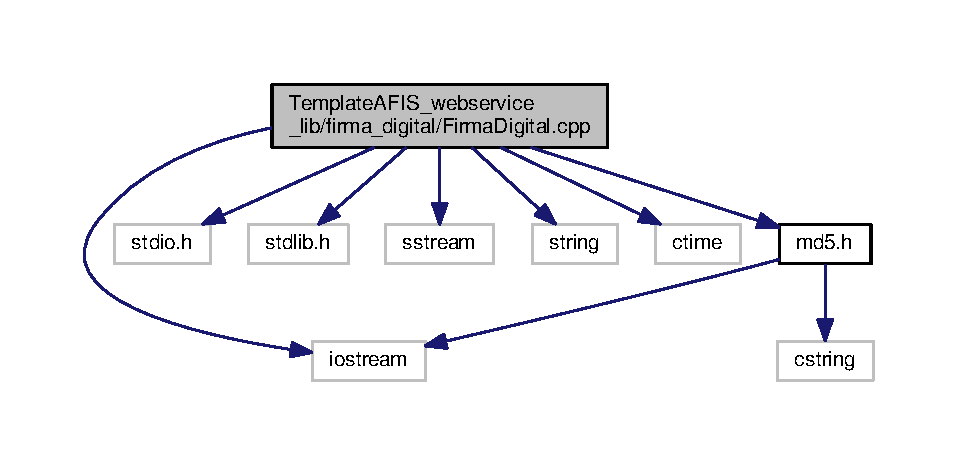
\includegraphics[width=350pt]{FirmaDigital_8cpp__incl}
\end{center}
\end{figure}


\subsection{Descripción detallada}
Se definen los métodos para generar la clave que será la firma de cada paquete X\+M\+L-\/\+R\+PC. 

Comando de compilación\+: g++ \hyperlink{sha512_8cpp}{sha512.\+cpp} firma\+\_\+srcl.\+cpp -\/o firma\+\_\+srcl \&\& ./firma\+\_\+srcl

\begin{DoxyAuthor}{Autor}
Asociación Cooperativa Simón Rodríguez para el Conocimiento Libre. \href{mailto:contacto@simonrodriguez.org.ve}{\tt contacto@simonrodriguez.\+org.\+ve} 
\end{DoxyAuthor}
\begin{DoxyDate}{Fecha}
2014 This file is part of Sistema de Identificación Biométrica para las O\+B\+PP. 
\end{DoxyDate}

\hypertarget{FirmaDigital_8h}{}\section{Referencia del Archivo Template\+A\+F\+I\+S\+\_\+webservice\+\_\+lib/firma\+\_\+digital/\+Firma\+Digital.h}
\label{FirmaDigital_8h}\index{Template\+A\+F\+I\+S\+\_\+webservice\+\_\+lib/firma\+\_\+digital/\+Firma\+Digital.\+h@{Template\+A\+F\+I\+S\+\_\+webservice\+\_\+lib/firma\+\_\+digital/\+Firma\+Digital.\+h}}


Archivo de cabecera de las clases \hyperlink{classFirmaDigital}{Firma\+Digital}.  


{\ttfamily \#include $<$string.\+h$>$}\newline
Dependencia gráfica adjunta para Firma\+Digital.\+h\+:\nopagebreak
\begin{figure}[H]
\begin{center}
\leavevmode
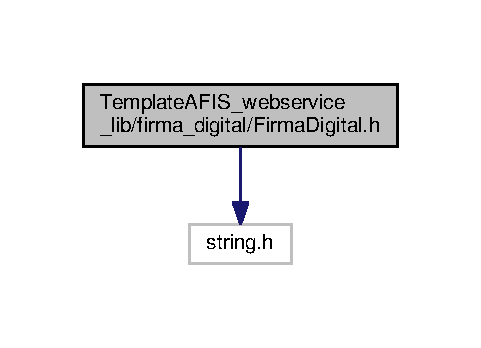
\includegraphics[width=231pt]{FirmaDigital_8h__incl}
\end{center}
\end{figure}
Gráfico de los archivos que directa o indirectamente incluyen a este archivo\+:\nopagebreak
\begin{figure}[H]
\begin{center}
\leavevmode
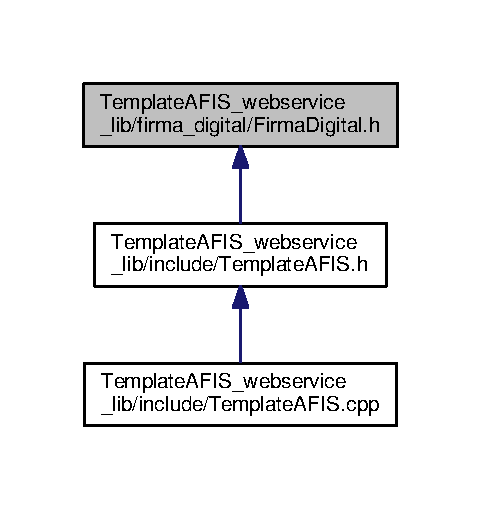
\includegraphics[width=231pt]{FirmaDigital_8h__dep__incl}
\end{center}
\end{figure}
\subsection*{Clases}
\begin{DoxyCompactItemize}
\item 
class \hyperlink{classFirmaDigital}{Firma\+Digital}
\begin{DoxyCompactList}\small\item\em Clase que permite realizar Firma Digital. \end{DoxyCompactList}\end{DoxyCompactItemize}


\subsection{Descripción detallada}
Archivo de cabecera de las clases \hyperlink{classFirmaDigital}{Firma\+Digital}. 

\begin{DoxyAuthor}{Autor}
Asociación Cooperativa Simón Rodríguez para el Conocimiento Libre, R.\+S. 
\end{DoxyAuthor}
\begin{DoxyDate}{Fecha}
2014 
\end{DoxyDate}
\begin{DoxyVersion}{Versión}
1.\+0
\end{DoxyVersion}
\href{mailto:contacto@simonrodriguez.org.ve}{\tt contacto@simonrodriguez.\+org.\+ve}

This file is part of Sistema de Identificación Biométrica para las O\+B\+PP. 
\hypertarget{md5_8cpp}{}\section{Referencia del Archivo Template\+A\+F\+I\+S\+\_\+webservice\+\_\+lib/firma\+\_\+digital/md5.cpp}
\label{md5_8cpp}\index{Template\+A\+F\+I\+S\+\_\+webservice\+\_\+lib/firma\+\_\+digital/md5.\+cpp@{Template\+A\+F\+I\+S\+\_\+webservice\+\_\+lib/firma\+\_\+digital/md5.\+cpp}}


Clase que se encarga de generar un hash alfanumérico de un tamaño predeterminado.  


{\ttfamily \#include \char`\"{}md5.\+h\char`\"{}}\newline
{\ttfamily \#include $<$cstdio$>$}\newline
Dependencia gráfica adjunta para md5.\+cpp\+:\nopagebreak
\begin{figure}[H]
\begin{center}
\leavevmode
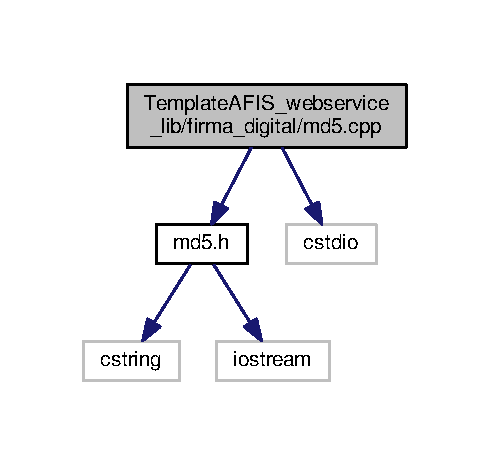
\includegraphics[width=235pt]{md5_8cpp__incl}
\end{center}
\end{figure}
\subsection*{\textquotesingle{}defines\textquotesingle{}}
\begin{DoxyCompactItemize}
\item 
\#define \hyperlink{md5_8cpp_a51398c0e5541164ad4d6615880073305}{S11}~7
\item 
\#define \hyperlink{md5_8cpp_a1ec499cd0e54ecc28c2ac2afea5b038e}{S12}~12
\item 
\#define \hyperlink{md5_8cpp_aaeec90429105fb54d853dd4fc7027a54}{S13}~17
\item 
\#define \hyperlink{md5_8cpp_a78342b0ccde2ed12fdf19a113cc266cf}{S14}~22
\item 
\#define \hyperlink{md5_8cpp_ab6d5354f647a0e7592a1f051fc8377b2}{S21}~5
\item 
\#define \hyperlink{md5_8cpp_addad30455da936bc1879ee9c72b46d59}{S22}~9
\item 
\#define \hyperlink{md5_8cpp_a6321a8b29628936f76e9e78cf5bda95f}{S23}~14
\item 
\#define \hyperlink{md5_8cpp_a0c09eb77d30a0d5f9154914147b86c20}{S24}~20
\item 
\#define \hyperlink{md5_8cpp_aef26590f8a880ee6f4a158168defcd89}{S31}~4
\item 
\#define \hyperlink{md5_8cpp_a1d512424dd8a91e0a5bcc98563f33914}{S32}~11
\item 
\#define \hyperlink{md5_8cpp_a1c854214533f6220e859b0063196abb3}{S33}~16
\item 
\#define \hyperlink{md5_8cpp_af6472be1d535970afee8e5266a74aa07}{S34}~23
\item 
\#define \hyperlink{md5_8cpp_ab674ba129e588da55d1d494e1cf3c15e}{S41}~6
\item 
\#define \hyperlink{md5_8cpp_a268ef1a49114a94b931cc6b313e3cd1b}{S42}~10
\item 
\#define \hyperlink{md5_8cpp_a5aaa7121f39650d472746942ca68f959}{S43}~15
\item 
\#define \hyperlink{md5_8cpp_a6a3989af72b55d169bd73a66f8620aae}{S44}~21
\end{DoxyCompactItemize}
\subsection*{Funciones}
\begin{DoxyCompactItemize}
\item 
std\+::ostream \& \hyperlink{md5_8cpp_a80cbf042ee22a0e557ac7938a6218e55}{operator$<$$<$} (std\+::ostream \&out, \hyperlink{classMD5}{M\+D5} \hyperlink{md5_8h_a92c6eed2e9b51298af559aff6792770b}{md5})
\item 
std\+::string \hyperlink{md5_8cpp_a92c6eed2e9b51298af559aff6792770b}{md5} (const std\+::string str)
\end{DoxyCompactItemize}


\subsection{Descripción detallada}
Clase que se encarga de generar un hash alfanumérico de un tamaño predeterminado. 

\begin{DoxyAuthor}{Autor}
Frank Thilo (\href{mailto:thilo@unix-ag.org}{\tt thilo@unix-\/ag.\+org}) This file is part of Sistema de Identificación Biométrica para las O\+B\+PP. 
\end{DoxyAuthor}


\subsection{Documentación de los \textquotesingle{}defines\textquotesingle{}}
\hypertarget{md5_8cpp_a51398c0e5541164ad4d6615880073305}{}\label{md5_8cpp_a51398c0e5541164ad4d6615880073305} 
\index{md5.\+cpp@{md5.\+cpp}!S11@{S11}}
\index{S11@{S11}!md5.\+cpp@{md5.\+cpp}}
\subsubsection{\texorpdfstring{S11}{S11}}
{\footnotesize\ttfamily \#define S11~7}



Definición en la línea 47 del archivo md5.\+cpp.



Referenciado por M\+D5\+::transform().

\hypertarget{md5_8cpp_a1ec499cd0e54ecc28c2ac2afea5b038e}{}\label{md5_8cpp_a1ec499cd0e54ecc28c2ac2afea5b038e} 
\index{md5.\+cpp@{md5.\+cpp}!S12@{S12}}
\index{S12@{S12}!md5.\+cpp@{md5.\+cpp}}
\subsubsection{\texorpdfstring{S12}{S12}}
{\footnotesize\ttfamily \#define S12~12}



Definición en la línea 48 del archivo md5.\+cpp.



Referenciado por M\+D5\+::transform().

\hypertarget{md5_8cpp_aaeec90429105fb54d853dd4fc7027a54}{}\label{md5_8cpp_aaeec90429105fb54d853dd4fc7027a54} 
\index{md5.\+cpp@{md5.\+cpp}!S13@{S13}}
\index{S13@{S13}!md5.\+cpp@{md5.\+cpp}}
\subsubsection{\texorpdfstring{S13}{S13}}
{\footnotesize\ttfamily \#define S13~17}



Definición en la línea 49 del archivo md5.\+cpp.



Referenciado por M\+D5\+::transform().

\hypertarget{md5_8cpp_a78342b0ccde2ed12fdf19a113cc266cf}{}\label{md5_8cpp_a78342b0ccde2ed12fdf19a113cc266cf} 
\index{md5.\+cpp@{md5.\+cpp}!S14@{S14}}
\index{S14@{S14}!md5.\+cpp@{md5.\+cpp}}
\subsubsection{\texorpdfstring{S14}{S14}}
{\footnotesize\ttfamily \#define S14~22}



Definición en la línea 50 del archivo md5.\+cpp.



Referenciado por M\+D5\+::transform().

\hypertarget{md5_8cpp_ab6d5354f647a0e7592a1f051fc8377b2}{}\label{md5_8cpp_ab6d5354f647a0e7592a1f051fc8377b2} 
\index{md5.\+cpp@{md5.\+cpp}!S21@{S21}}
\index{S21@{S21}!md5.\+cpp@{md5.\+cpp}}
\subsubsection{\texorpdfstring{S21}{S21}}
{\footnotesize\ttfamily \#define S21~5}



Definición en la línea 51 del archivo md5.\+cpp.



Referenciado por M\+D5\+::transform().

\hypertarget{md5_8cpp_addad30455da936bc1879ee9c72b46d59}{}\label{md5_8cpp_addad30455da936bc1879ee9c72b46d59} 
\index{md5.\+cpp@{md5.\+cpp}!S22@{S22}}
\index{S22@{S22}!md5.\+cpp@{md5.\+cpp}}
\subsubsection{\texorpdfstring{S22}{S22}}
{\footnotesize\ttfamily \#define S22~9}



Definición en la línea 52 del archivo md5.\+cpp.



Referenciado por M\+D5\+::transform().

\hypertarget{md5_8cpp_a6321a8b29628936f76e9e78cf5bda95f}{}\label{md5_8cpp_a6321a8b29628936f76e9e78cf5bda95f} 
\index{md5.\+cpp@{md5.\+cpp}!S23@{S23}}
\index{S23@{S23}!md5.\+cpp@{md5.\+cpp}}
\subsubsection{\texorpdfstring{S23}{S23}}
{\footnotesize\ttfamily \#define S23~14}



Definición en la línea 53 del archivo md5.\+cpp.



Referenciado por M\+D5\+::transform().

\hypertarget{md5_8cpp_a0c09eb77d30a0d5f9154914147b86c20}{}\label{md5_8cpp_a0c09eb77d30a0d5f9154914147b86c20} 
\index{md5.\+cpp@{md5.\+cpp}!S24@{S24}}
\index{S24@{S24}!md5.\+cpp@{md5.\+cpp}}
\subsubsection{\texorpdfstring{S24}{S24}}
{\footnotesize\ttfamily \#define S24~20}



Definición en la línea 54 del archivo md5.\+cpp.



Referenciado por M\+D5\+::transform().

\hypertarget{md5_8cpp_aef26590f8a880ee6f4a158168defcd89}{}\label{md5_8cpp_aef26590f8a880ee6f4a158168defcd89} 
\index{md5.\+cpp@{md5.\+cpp}!S31@{S31}}
\index{S31@{S31}!md5.\+cpp@{md5.\+cpp}}
\subsubsection{\texorpdfstring{S31}{S31}}
{\footnotesize\ttfamily \#define S31~4}



Definición en la línea 55 del archivo md5.\+cpp.



Referenciado por M\+D5\+::transform().

\hypertarget{md5_8cpp_a1d512424dd8a91e0a5bcc98563f33914}{}\label{md5_8cpp_a1d512424dd8a91e0a5bcc98563f33914} 
\index{md5.\+cpp@{md5.\+cpp}!S32@{S32}}
\index{S32@{S32}!md5.\+cpp@{md5.\+cpp}}
\subsubsection{\texorpdfstring{S32}{S32}}
{\footnotesize\ttfamily \#define S32~11}



Definición en la línea 56 del archivo md5.\+cpp.



Referenciado por M\+D5\+::transform().

\hypertarget{md5_8cpp_a1c854214533f6220e859b0063196abb3}{}\label{md5_8cpp_a1c854214533f6220e859b0063196abb3} 
\index{md5.\+cpp@{md5.\+cpp}!S33@{S33}}
\index{S33@{S33}!md5.\+cpp@{md5.\+cpp}}
\subsubsection{\texorpdfstring{S33}{S33}}
{\footnotesize\ttfamily \#define S33~16}



Definición en la línea 57 del archivo md5.\+cpp.



Referenciado por M\+D5\+::transform().

\hypertarget{md5_8cpp_af6472be1d535970afee8e5266a74aa07}{}\label{md5_8cpp_af6472be1d535970afee8e5266a74aa07} 
\index{md5.\+cpp@{md5.\+cpp}!S34@{S34}}
\index{S34@{S34}!md5.\+cpp@{md5.\+cpp}}
\subsubsection{\texorpdfstring{S34}{S34}}
{\footnotesize\ttfamily \#define S34~23}



Definición en la línea 58 del archivo md5.\+cpp.



Referenciado por M\+D5\+::transform().

\hypertarget{md5_8cpp_ab674ba129e588da55d1d494e1cf3c15e}{}\label{md5_8cpp_ab674ba129e588da55d1d494e1cf3c15e} 
\index{md5.\+cpp@{md5.\+cpp}!S41@{S41}}
\index{S41@{S41}!md5.\+cpp@{md5.\+cpp}}
\subsubsection{\texorpdfstring{S41}{S41}}
{\footnotesize\ttfamily \#define S41~6}



Definición en la línea 59 del archivo md5.\+cpp.



Referenciado por M\+D5\+::transform().

\hypertarget{md5_8cpp_a268ef1a49114a94b931cc6b313e3cd1b}{}\label{md5_8cpp_a268ef1a49114a94b931cc6b313e3cd1b} 
\index{md5.\+cpp@{md5.\+cpp}!S42@{S42}}
\index{S42@{S42}!md5.\+cpp@{md5.\+cpp}}
\subsubsection{\texorpdfstring{S42}{S42}}
{\footnotesize\ttfamily \#define S42~10}



Definición en la línea 60 del archivo md5.\+cpp.



Referenciado por M\+D5\+::transform().

\hypertarget{md5_8cpp_a5aaa7121f39650d472746942ca68f959}{}\label{md5_8cpp_a5aaa7121f39650d472746942ca68f959} 
\index{md5.\+cpp@{md5.\+cpp}!S43@{S43}}
\index{S43@{S43}!md5.\+cpp@{md5.\+cpp}}
\subsubsection{\texorpdfstring{S43}{S43}}
{\footnotesize\ttfamily \#define S43~15}



Definición en la línea 61 del archivo md5.\+cpp.



Referenciado por M\+D5\+::transform().

\hypertarget{md5_8cpp_a6a3989af72b55d169bd73a66f8620aae}{}\label{md5_8cpp_a6a3989af72b55d169bd73a66f8620aae} 
\index{md5.\+cpp@{md5.\+cpp}!S44@{S44}}
\index{S44@{S44}!md5.\+cpp@{md5.\+cpp}}
\subsubsection{\texorpdfstring{S44}{S44}}
{\footnotesize\ttfamily \#define S44~21}



Definición en la línea 62 del archivo md5.\+cpp.



Referenciado por M\+D5\+::transform().



\subsection{Documentación de las funciones}
\hypertarget{md5_8cpp_a92c6eed2e9b51298af559aff6792770b}{}\label{md5_8cpp_a92c6eed2e9b51298af559aff6792770b} 
\index{md5.\+cpp@{md5.\+cpp}!md5@{md5}}
\index{md5@{md5}!md5.\+cpp@{md5.\+cpp}}
\subsubsection{\texorpdfstring{md5()}{md5()}}
{\footnotesize\ttfamily std\+::string md5 (\begin{DoxyParamCaption}\item[{const std\+::string}]{str }\end{DoxyParamCaption})}



Definición en la línea 351 del archivo md5.\+cpp.



Hace referencia a M\+D5\+::hexdigest(), M\+D5\+::\+M\+D5() y md5().



Referenciado por Firma\+Digital\+::firma\+\_\+srcl() y md5().

Gráfico de llamadas para esta función\+:\nopagebreak
\begin{figure}[H]
\begin{center}
\leavevmode
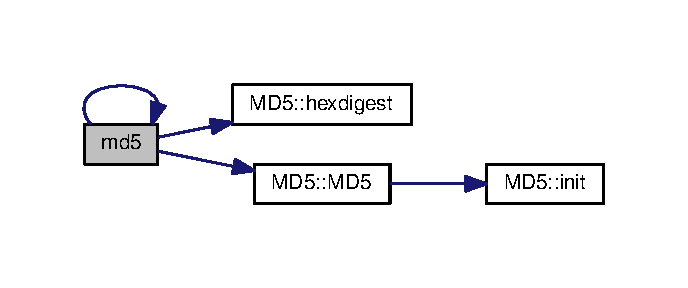
\includegraphics[width=330pt]{md5_8cpp_a92c6eed2e9b51298af559aff6792770b_cgraph}
\end{center}
\end{figure}
\hypertarget{md5_8cpp_a80cbf042ee22a0e557ac7938a6218e55}{}\label{md5_8cpp_a80cbf042ee22a0e557ac7938a6218e55} 
\index{md5.\+cpp@{md5.\+cpp}!operator$<$$<$@{operator$<$$<$}}
\index{operator$<$$<$@{operator$<$$<$}!md5.\+cpp@{md5.\+cpp}}
\subsubsection{\texorpdfstring{operator$<$$<$()}{operator<<()}}
{\footnotesize\ttfamily std\+::ostream\& operator$<$$<$ (\begin{DoxyParamCaption}\item[{std\+::ostream \&}]{out,  }\item[{\hyperlink{classMD5}{M\+D5}}]{md5 }\end{DoxyParamCaption})}



Definición en la línea 344 del archivo md5.\+cpp.



Hace referencia a M\+D5\+::hexdigest().

Gráfico de llamadas para esta función\+:\nopagebreak
\begin{figure}[H]
\begin{center}
\leavevmode
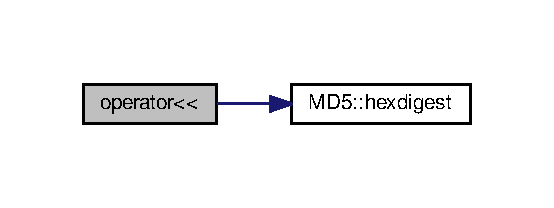
\includegraphics[width=266pt]{md5_8cpp_a80cbf042ee22a0e557ac7938a6218e55_cgraph}
\end{center}
\end{figure}

\hypertarget{md5_8h}{}\section{Referencia del Archivo Template\+A\+F\+I\+S\+\_\+webservice\+\_\+lib/firma\+\_\+digital/md5.h}
\label{md5_8h}\index{Template\+A\+F\+I\+S\+\_\+webservice\+\_\+lib/firma\+\_\+digital/md5.\+h@{Template\+A\+F\+I\+S\+\_\+webservice\+\_\+lib/firma\+\_\+digital/md5.\+h}}


Clase cabecera que se encarga de generar un hash alfanumérico de un tamaño predeterminado.  


{\ttfamily \#include $<$cstring$>$}\newline
{\ttfamily \#include $<$iostream$>$}\newline
Dependencia gráfica adjunta para md5.\+h\+:\nopagebreak
\begin{figure}[H]
\begin{center}
\leavevmode
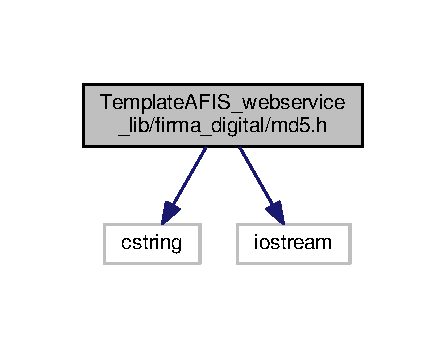
\includegraphics[width=214pt]{md5_8h__incl}
\end{center}
\end{figure}
Gráfico de los archivos que directa o indirectamente incluyen a este archivo\+:\nopagebreak
\begin{figure}[H]
\begin{center}
\leavevmode
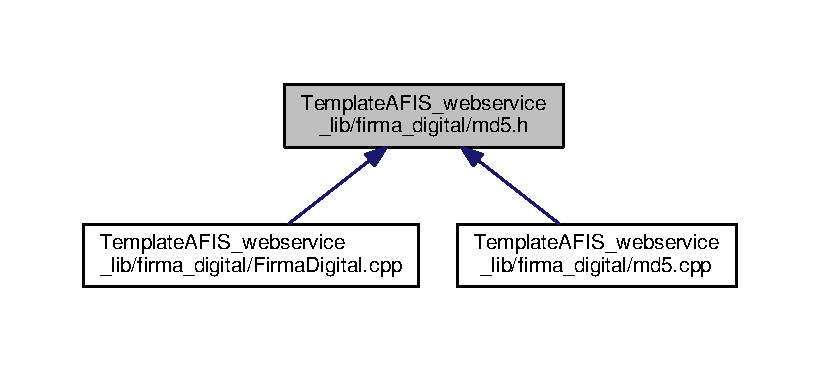
\includegraphics[width=350pt]{md5_8h__dep__incl}
\end{center}
\end{figure}
\subsection*{Clases}
\begin{DoxyCompactItemize}
\item 
class \hyperlink{classMD5}{M\+D5}
\begin{DoxyCompactList}\small\item\em Clase de la comunidad\+: Se encarga de generar un hash alfanumérico de un tamaño predeterminado, no importa cuál sea la entrada que le suministren. Es igual al que se usa para comparar dos archivos, o en encriptación. Se incluye en la compilación para evitar que un cambio de versión en el sistema de operación de una máquina pudiese afectar la comunicación. (Recibe la información de \hyperlink{FirmaDigital_8cpp}{Firma\+Digital.\+cpp} y crea los hash correspondientes para encriptarlo en \hyperlink{sha512_8cpp}{sha512.\+cpp}) \end{DoxyCompactList}\end{DoxyCompactItemize}
\subsection*{Funciones}
\begin{DoxyCompactItemize}
\item 
std\+::string \hyperlink{md5_8h_a92c6eed2e9b51298af559aff6792770b}{md5} (const std\+::string str)
\end{DoxyCompactItemize}


\subsection{Descripción detallada}
Clase cabecera que se encarga de generar un hash alfanumérico de un tamaño predeterminado. 

\begin{DoxyAuthor}{Autor}
Frank Thilo (\href{mailto:thilo@unix-ag.org}{\tt thilo@unix-\/ag.\+org}) This file is part of Sistema de Identificación Biométrica para las O\+B\+PP. 
\end{DoxyAuthor}


\subsection{Documentación de las funciones}
\hypertarget{md5_8h_a92c6eed2e9b51298af559aff6792770b}{}\label{md5_8h_a92c6eed2e9b51298af559aff6792770b} 
\index{md5.\+h@{md5.\+h}!md5@{md5}}
\index{md5@{md5}!md5.\+h@{md5.\+h}}
\subsubsection{\texorpdfstring{md5()}{md5()}}
{\footnotesize\ttfamily std\+::string md5 (\begin{DoxyParamCaption}\item[{const std\+::string}]{str }\end{DoxyParamCaption})}



Definición en la línea 351 del archivo md5.\+cpp.



Hace referencia a M\+D5\+::hexdigest(), M\+D5\+::\+M\+D5() y md5().



Referenciado por Firma\+Digital\+::firma\+\_\+srcl() y md5().

Gráfico de llamadas para esta función\+:\nopagebreak
\begin{figure}[H]
\begin{center}
\leavevmode
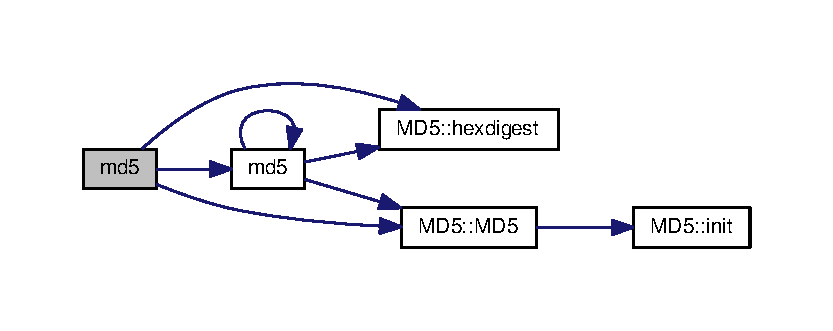
\includegraphics[width=350pt]{md5_8h_a92c6eed2e9b51298af559aff6792770b_cgraph}
\end{center}
\end{figure}

\hypertarget{sha512_8cpp}{}\section{Referencia del Archivo Template\+A\+F\+I\+S\+\_\+webservice\+\_\+lib/firma\+\_\+digital/sha512.cpp}
\label{sha512_8cpp}\index{Template\+A\+F\+I\+S\+\_\+webservice\+\_\+lib/firma\+\_\+digital/sha512.\+cpp@{Template\+A\+F\+I\+S\+\_\+webservice\+\_\+lib/firma\+\_\+digital/sha512.\+cpp}}


Clase cabecera para estabilizar la clase \hyperlink{md5_8cpp}{md5.\+cpp} por versiones diferentes de las bibliotecas de \hyperlink{classMD5}{M\+D5} o de \hyperlink{classSHA512}{S\+H\+A512} en el servidor.  


{\ttfamily \#include $<$cstring$>$}\newline
{\ttfamily \#include $<$fstream$>$}\newline
{\ttfamily \#include \char`\"{}sha512.\+h\char`\"{}}\newline
Dependencia gráfica adjunta para sha512.\+cpp\+:\nopagebreak
\begin{figure}[H]
\begin{center}
\leavevmode
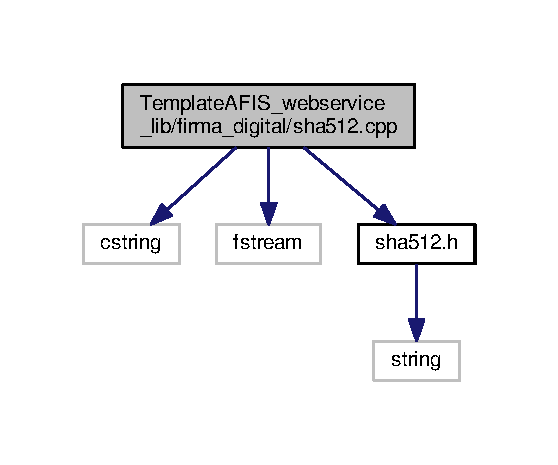
\includegraphics[width=268pt]{sha512_8cpp__incl}
\end{center}
\end{figure}
\subsection*{Funciones}
\begin{DoxyCompactItemize}
\item 
std\+::string \hyperlink{sha512_8cpp_acab52167a6e7f6daf06e9cbeae13aae6}{sha512} (std\+::string input)
\end{DoxyCompactItemize}


\subsection{Descripción detallada}
Clase cabecera para estabilizar la clase \hyperlink{md5_8cpp}{md5.\+cpp} por versiones diferentes de las bibliotecas de \hyperlink{classMD5}{M\+D5} o de \hyperlink{classSHA512}{S\+H\+A512} en el servidor. 

\begin{DoxyAuthor}{Autor}
\href{http://www.zedwood.com/article/cpp-sha512-function}{\tt http\+://www.\+zedwood.\+com/article/cpp-\/sha512-\/function} This file is part of Sistema de Identificación Biométrica para las O\+B\+PP. 
\end{DoxyAuthor}


\subsection{Documentación de las funciones}
\hypertarget{sha512_8cpp_acab52167a6e7f6daf06e9cbeae13aae6}{}\label{sha512_8cpp_acab52167a6e7f6daf06e9cbeae13aae6} 
\index{sha512.\+cpp@{sha512.\+cpp}!sha512@{sha512}}
\index{sha512@{sha512}!sha512.\+cpp@{sha512.\+cpp}}
\subsubsection{\texorpdfstring{sha512()}{sha512()}}
{\footnotesize\ttfamily std\+::string sha512 (\begin{DoxyParamCaption}\item[{std\+::string}]{input }\end{DoxyParamCaption})}



Definición en la línea 149 del archivo sha512.\+cpp.



Hace referencia a S\+H\+A512\+::\+D\+I\+G\+E\+S\+T\+\_\+\+S\+I\+ZE, S\+H\+A512\+::final(), S\+H\+A512\+::init() y S\+H\+A512\+::update().

Gráfico de llamadas para esta función\+:\nopagebreak
\begin{figure}[H]
\begin{center}
\leavevmode
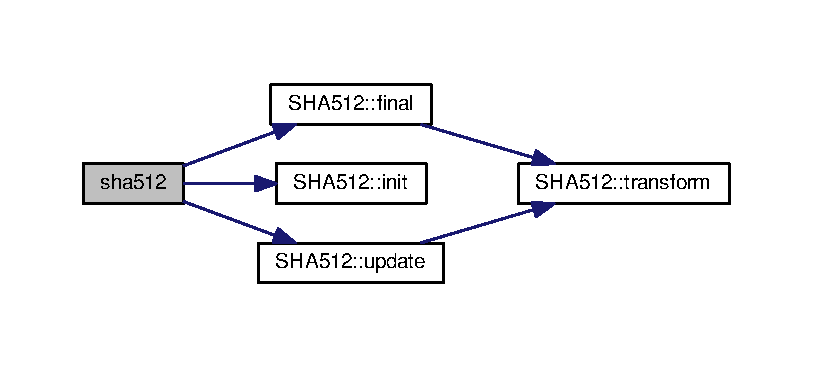
\includegraphics[width=350pt]{sha512_8cpp_acab52167a6e7f6daf06e9cbeae13aae6_cgraph}
\end{center}
\end{figure}

\hypertarget{sha512_8h}{}\section{Referencia del Archivo Template\+A\+F\+I\+S\+\_\+webservice\+\_\+lib/firma\+\_\+digital/sha512.h}
\label{sha512_8h}\index{Template\+A\+F\+I\+S\+\_\+webservice\+\_\+lib/firma\+\_\+digital/sha512.\+h@{Template\+A\+F\+I\+S\+\_\+webservice\+\_\+lib/firma\+\_\+digital/sha512.\+h}}


Clase cabecera para estabilizar la clase \hyperlink{md5_8cpp}{md5.\+cpp} por versiones diferentes de las bibliotecas de \hyperlink{classMD5}{M\+D5} o de \hyperlink{classSHA512}{S\+H\+A512} en el servidor.  


{\ttfamily \#include $<$string$>$}\newline
Dependencia gráfica adjunta para sha512.\+h\+:\nopagebreak
\begin{figure}[H]
\begin{center}
\leavevmode
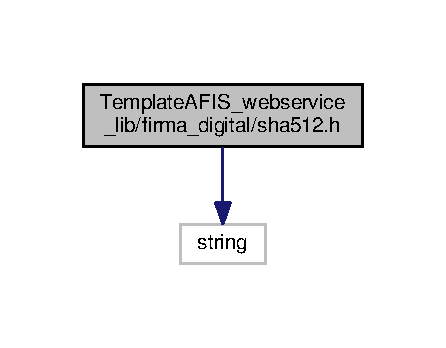
\includegraphics[width=214pt]{sha512_8h__incl}
\end{center}
\end{figure}
Gráfico de los archivos que directa o indirectamente incluyen a este archivo\+:\nopagebreak
\begin{figure}[H]
\begin{center}
\leavevmode
\includegraphics[width=220pt]{sha512_8h__dep__incl}
\end{center}
\end{figure}
\subsection*{Clases}
\begin{DoxyCompactItemize}
\item 
class \hyperlink{classSHA512}{S\+H\+A512}
\begin{DoxyCompactList}\small\item\em Clase de la comunidad\+: Se incluyó para estabilizar \hyperlink{md5_8cpp}{md5.\+cpp} para evitar que, si el cliente tiene una versión diferente de las bibliotecas de \hyperlink{classMD5}{M\+D5} o de \hyperlink{classSHA512}{S\+H\+A512} que el servidor, no choquen. \end{DoxyCompactList}\end{DoxyCompactItemize}
\subsection*{\textquotesingle{}defines\textquotesingle{}}
\begin{DoxyCompactItemize}
\item 
\#define \hyperlink{sha512_8h_a0a0e7e0d135e9feff1da2e46fa556d50}{S\+H\+A2\+\_\+\+S\+H\+FR}(x,  n)~(x $>$$>$ n)
\item 
\#define \hyperlink{sha512_8h_a9509f7c1f927cb12f98d9995ae2f92d3}{S\+H\+A2\+\_\+\+R\+O\+TR}(x,  n)~((x $>$$>$ n) $\vert$ (x $<$$<$ ((sizeof(x) $<$$<$ 3) -\/ n)))
\item 
\#define \hyperlink{sha512_8h_a0fcefdff5f2609b2c5eb1d0f99214199}{S\+H\+A2\+\_\+\+R\+O\+TL}(x,  n)~((x $<$$<$ n) $\vert$ (x $>$$>$ ((sizeof(x) $<$$<$ 3) -\/ n)))
\item 
\#define \hyperlink{sha512_8h_a1d4a72c3cb3d85b0c82736081042c1a4}{S\+H\+A2\+\_\+\+CH}(x,  y,  z)~((x \& y) $^\wedge$ ($\sim$x \& z))
\item 
\#define \hyperlink{sha512_8h_ae9222f6c22449097806fb1dac2a58107}{S\+H\+A2\+\_\+\+M\+AJ}(x,  y,  z)~((x \& y) $^\wedge$ (x \& z) $^\wedge$ (y \& z))
\item 
\#define \hyperlink{sha512_8h_a8c65d2c0860cf623b5607b2aec6a870a}{S\+H\+A512\+\_\+\+F1}(x)~(\hyperlink{sha512_8h_a9509f7c1f927cb12f98d9995ae2f92d3}{S\+H\+A2\+\_\+\+R\+O\+TR}(x, 28) $^\wedge$ \hyperlink{sha512_8h_a9509f7c1f927cb12f98d9995ae2f92d3}{S\+H\+A2\+\_\+\+R\+O\+TR}(x, 34) $^\wedge$ \hyperlink{sha512_8h_a9509f7c1f927cb12f98d9995ae2f92d3}{S\+H\+A2\+\_\+\+R\+O\+TR}(x, 39))
\item 
\#define \hyperlink{sha512_8h_a41b8a672f8ed1a11ea49acb032550fa6}{S\+H\+A512\+\_\+\+F2}(x)~(\hyperlink{sha512_8h_a9509f7c1f927cb12f98d9995ae2f92d3}{S\+H\+A2\+\_\+\+R\+O\+TR}(x, 14) $^\wedge$ \hyperlink{sha512_8h_a9509f7c1f927cb12f98d9995ae2f92d3}{S\+H\+A2\+\_\+\+R\+O\+TR}(x, 18) $^\wedge$ \hyperlink{sha512_8h_a9509f7c1f927cb12f98d9995ae2f92d3}{S\+H\+A2\+\_\+\+R\+O\+TR}(x, 41))
\item 
\#define \hyperlink{sha512_8h_a278e83abc8c71fec8a719065e5d51106}{S\+H\+A512\+\_\+\+F3}(x)~(\hyperlink{sha512_8h_a9509f7c1f927cb12f98d9995ae2f92d3}{S\+H\+A2\+\_\+\+R\+O\+TR}(x,  1) $^\wedge$ \hyperlink{sha512_8h_a9509f7c1f927cb12f98d9995ae2f92d3}{S\+H\+A2\+\_\+\+R\+O\+TR}(x,  8) $^\wedge$ \hyperlink{sha512_8h_a0a0e7e0d135e9feff1da2e46fa556d50}{S\+H\+A2\+\_\+\+S\+H\+FR}(x,  7))
\item 
\#define \hyperlink{sha512_8h_ad6d26f67626668a9ec4f113bd05bee2b}{S\+H\+A512\+\_\+\+F4}(x)~(\hyperlink{sha512_8h_a9509f7c1f927cb12f98d9995ae2f92d3}{S\+H\+A2\+\_\+\+R\+O\+TR}(x, 19) $^\wedge$ \hyperlink{sha512_8h_a9509f7c1f927cb12f98d9995ae2f92d3}{S\+H\+A2\+\_\+\+R\+O\+TR}(x, 61) $^\wedge$ \hyperlink{sha512_8h_a0a0e7e0d135e9feff1da2e46fa556d50}{S\+H\+A2\+\_\+\+S\+H\+FR}(x,  6))
\item 
\#define \hyperlink{sha512_8h_a2dc032adc83afe8e265a7941ef11f258}{S\+H\+A2\+\_\+\+U\+N\+P\+A\+C\+K32}(x,  str)
\item 
\#define \hyperlink{sha512_8h_a81e6dc4766f3664c56beb47948d35e23}{S\+H\+A2\+\_\+\+U\+N\+P\+A\+C\+K64}(x,  str)
\item 
\#define \hyperlink{sha512_8h_abfcad1e5762f93ffd8cd566bbe261a19}{S\+H\+A2\+\_\+\+P\+A\+C\+K64}(str,  x)
\end{DoxyCompactItemize}
\subsection*{Funciones}
\begin{DoxyCompactItemize}
\item 
std\+::string \hyperlink{sha512_8h_acab52167a6e7f6daf06e9cbeae13aae6}{sha512} (std\+::string input)
\end{DoxyCompactItemize}


\subsection{Descripción detallada}
Clase cabecera para estabilizar la clase \hyperlink{md5_8cpp}{md5.\+cpp} por versiones diferentes de las bibliotecas de \hyperlink{classMD5}{M\+D5} o de \hyperlink{classSHA512}{S\+H\+A512} en el servidor. 

\begin{DoxyAuthor}{Autor}
\href{http://www.zedwood.com/article/cpp-sha512-function}{\tt http\+://www.\+zedwood.\+com/article/cpp-\/sha512-\/function} This file is part of Sistema de Identificación Biométrica para las O\+B\+PP. 
\end{DoxyAuthor}


\subsection{Documentación de los \textquotesingle{}defines\textquotesingle{}}
\hypertarget{sha512_8h_a1d4a72c3cb3d85b0c82736081042c1a4}{}\label{sha512_8h_a1d4a72c3cb3d85b0c82736081042c1a4} 
\index{sha512.\+h@{sha512.\+h}!S\+H\+A2\+\_\+\+CH@{S\+H\+A2\+\_\+\+CH}}
\index{S\+H\+A2\+\_\+\+CH@{S\+H\+A2\+\_\+\+CH}!sha512.\+h@{sha512.\+h}}
\subsubsection{\texorpdfstring{S\+H\+A2\+\_\+\+CH}{SHA2\_CH}}
{\footnotesize\ttfamily \#define S\+H\+A2\+\_\+\+CH(\begin{DoxyParamCaption}\item[{}]{x,  }\item[{}]{y,  }\item[{}]{z }\end{DoxyParamCaption})~((x \& y) $^\wedge$ ($\sim$x \& z))}



Definición en la línea 90 del archivo sha512.\+h.



Referenciado por S\+H\+A512\+::transform().

\hypertarget{sha512_8h_ae9222f6c22449097806fb1dac2a58107}{}\label{sha512_8h_ae9222f6c22449097806fb1dac2a58107} 
\index{sha512.\+h@{sha512.\+h}!S\+H\+A2\+\_\+\+M\+AJ@{S\+H\+A2\+\_\+\+M\+AJ}}
\index{S\+H\+A2\+\_\+\+M\+AJ@{S\+H\+A2\+\_\+\+M\+AJ}!sha512.\+h@{sha512.\+h}}
\subsubsection{\texorpdfstring{S\+H\+A2\+\_\+\+M\+AJ}{SHA2\_MAJ}}
{\footnotesize\ttfamily \#define S\+H\+A2\+\_\+\+M\+AJ(\begin{DoxyParamCaption}\item[{}]{x,  }\item[{}]{y,  }\item[{}]{z }\end{DoxyParamCaption})~((x \& y) $^\wedge$ (x \& z) $^\wedge$ (y \& z))}



Definición en la línea 91 del archivo sha512.\+h.



Referenciado por S\+H\+A512\+::transform().

\hypertarget{sha512_8h_abfcad1e5762f93ffd8cd566bbe261a19}{}\label{sha512_8h_abfcad1e5762f93ffd8cd566bbe261a19} 
\index{sha512.\+h@{sha512.\+h}!S\+H\+A2\+\_\+\+P\+A\+C\+K64@{S\+H\+A2\+\_\+\+P\+A\+C\+K64}}
\index{S\+H\+A2\+\_\+\+P\+A\+C\+K64@{S\+H\+A2\+\_\+\+P\+A\+C\+K64}!sha512.\+h@{sha512.\+h}}
\subsubsection{\texorpdfstring{S\+H\+A2\+\_\+\+P\+A\+C\+K64}{SHA2\_PACK64}}
{\footnotesize\ttfamily \#define S\+H\+A2\+\_\+\+P\+A\+C\+K64(\begin{DoxyParamCaption}\item[{}]{str,  }\item[{}]{x }\end{DoxyParamCaption})}

{\bfseries Valor\+:}
\begin{DoxyCode}
\{                                             \(\backslash\)
    *(x) =   ((uint64) *((str) + 7)      )    \(\backslash\)
           | ((uint64) *((str) + 6) <<  8)    \(\backslash\)
           | ((uint64) *((str) + 5) << 16)    \(\backslash\)
           | ((uint64) *((str) + 4) << 24)    \(\backslash\)
           | ((uint64) *((str) + 3) << 32)    \(\backslash\)
           | ((uint64) *((str) + 2) << 40)    \(\backslash\)
           | ((uint64) *((str) + 1) << 48)    \(\backslash\)
           | ((uint64) *((str) + 0) << 56);   \(\backslash\)
\}
\end{DoxyCode}


Definición en la línea 114 del archivo sha512.\+h.



Referenciado por S\+H\+A512\+::transform().

\hypertarget{sha512_8h_a0fcefdff5f2609b2c5eb1d0f99214199}{}\label{sha512_8h_a0fcefdff5f2609b2c5eb1d0f99214199} 
\index{sha512.\+h@{sha512.\+h}!S\+H\+A2\+\_\+\+R\+O\+TL@{S\+H\+A2\+\_\+\+R\+O\+TL}}
\index{S\+H\+A2\+\_\+\+R\+O\+TL@{S\+H\+A2\+\_\+\+R\+O\+TL}!sha512.\+h@{sha512.\+h}}
\subsubsection{\texorpdfstring{S\+H\+A2\+\_\+\+R\+O\+TL}{SHA2\_ROTL}}
{\footnotesize\ttfamily \#define S\+H\+A2\+\_\+\+R\+O\+TL(\begin{DoxyParamCaption}\item[{}]{x,  }\item[{}]{n }\end{DoxyParamCaption})~((x $<$$<$ n) $\vert$ (x $>$$>$ ((sizeof(x) $<$$<$ 3) -\/ n)))}



Definición en la línea 89 del archivo sha512.\+h.

\hypertarget{sha512_8h_a9509f7c1f927cb12f98d9995ae2f92d3}{}\label{sha512_8h_a9509f7c1f927cb12f98d9995ae2f92d3} 
\index{sha512.\+h@{sha512.\+h}!S\+H\+A2\+\_\+\+R\+O\+TR@{S\+H\+A2\+\_\+\+R\+O\+TR}}
\index{S\+H\+A2\+\_\+\+R\+O\+TR@{S\+H\+A2\+\_\+\+R\+O\+TR}!sha512.\+h@{sha512.\+h}}
\subsubsection{\texorpdfstring{S\+H\+A2\+\_\+\+R\+O\+TR}{SHA2\_ROTR}}
{\footnotesize\ttfamily \#define S\+H\+A2\+\_\+\+R\+O\+TR(\begin{DoxyParamCaption}\item[{}]{x,  }\item[{}]{n }\end{DoxyParamCaption})~((x $>$$>$ n) $\vert$ (x $<$$<$ ((sizeof(x) $<$$<$ 3) -\/ n)))}



Definición en la línea 88 del archivo sha512.\+h.

\hypertarget{sha512_8h_a0a0e7e0d135e9feff1da2e46fa556d50}{}\label{sha512_8h_a0a0e7e0d135e9feff1da2e46fa556d50} 
\index{sha512.\+h@{sha512.\+h}!S\+H\+A2\+\_\+\+S\+H\+FR@{S\+H\+A2\+\_\+\+S\+H\+FR}}
\index{S\+H\+A2\+\_\+\+S\+H\+FR@{S\+H\+A2\+\_\+\+S\+H\+FR}!sha512.\+h@{sha512.\+h}}
\subsubsection{\texorpdfstring{S\+H\+A2\+\_\+\+S\+H\+FR}{SHA2\_SHFR}}
{\footnotesize\ttfamily \#define S\+H\+A2\+\_\+\+S\+H\+FR(\begin{DoxyParamCaption}\item[{}]{x,  }\item[{}]{n }\end{DoxyParamCaption})~(x $>$$>$ n)}



Definición en la línea 87 del archivo sha512.\+h.

\hypertarget{sha512_8h_a2dc032adc83afe8e265a7941ef11f258}{}\label{sha512_8h_a2dc032adc83afe8e265a7941ef11f258} 
\index{sha512.\+h@{sha512.\+h}!S\+H\+A2\+\_\+\+U\+N\+P\+A\+C\+K32@{S\+H\+A2\+\_\+\+U\+N\+P\+A\+C\+K32}}
\index{S\+H\+A2\+\_\+\+U\+N\+P\+A\+C\+K32@{S\+H\+A2\+\_\+\+U\+N\+P\+A\+C\+K32}!sha512.\+h@{sha512.\+h}}
\subsubsection{\texorpdfstring{S\+H\+A2\+\_\+\+U\+N\+P\+A\+C\+K32}{SHA2\_UNPACK32}}
{\footnotesize\ttfamily \#define S\+H\+A2\+\_\+\+U\+N\+P\+A\+C\+K32(\begin{DoxyParamCaption}\item[{}]{x,  }\item[{}]{str }\end{DoxyParamCaption})}

{\bfseries Valor\+:}
\begin{DoxyCode}
\{                                             \(\backslash\)
    *((str) + 3) = (uint8) ((x)      );       \(\backslash\)
    *((str) + 2) = (uint8) ((x) >>  8);       \(\backslash\)
    *((str) + 1) = (uint8) ((x) >> 16);       \(\backslash\)
    *((str) + 0) = (uint8) ((x) >> 24);       \(\backslash\)
\}
\end{DoxyCode}


Definición en la línea 96 del archivo sha512.\+h.



Referenciado por S\+H\+A512\+::final().

\hypertarget{sha512_8h_a81e6dc4766f3664c56beb47948d35e23}{}\label{sha512_8h_a81e6dc4766f3664c56beb47948d35e23} 
\index{sha512.\+h@{sha512.\+h}!S\+H\+A2\+\_\+\+U\+N\+P\+A\+C\+K64@{S\+H\+A2\+\_\+\+U\+N\+P\+A\+C\+K64}}
\index{S\+H\+A2\+\_\+\+U\+N\+P\+A\+C\+K64@{S\+H\+A2\+\_\+\+U\+N\+P\+A\+C\+K64}!sha512.\+h@{sha512.\+h}}
\subsubsection{\texorpdfstring{S\+H\+A2\+\_\+\+U\+N\+P\+A\+C\+K64}{SHA2\_UNPACK64}}
{\footnotesize\ttfamily \#define S\+H\+A2\+\_\+\+U\+N\+P\+A\+C\+K64(\begin{DoxyParamCaption}\item[{}]{x,  }\item[{}]{str }\end{DoxyParamCaption})}

{\bfseries Valor\+:}
\begin{DoxyCode}
\{                                             \(\backslash\)
    *((str) + 7) = (uint8) ((x)      );       \(\backslash\)
    *((str) + 6) = (uint8) ((x) >>  8);       \(\backslash\)
    *((str) + 5) = (uint8) ((x) >> 16);       \(\backslash\)
    *((str) + 4) = (uint8) ((x) >> 24);       \(\backslash\)
    *((str) + 3) = (uint8) ((x) >> 32);       \(\backslash\)
    *((str) + 2) = (uint8) ((x) >> 40);       \(\backslash\)
    *((str) + 1) = (uint8) ((x) >> 48);       \(\backslash\)
    *((str) + 0) = (uint8) ((x) >> 56);       \(\backslash\)
\}
\end{DoxyCode}


Definición en la línea 103 del archivo sha512.\+h.



Referenciado por S\+H\+A512\+::final().

\hypertarget{sha512_8h_a8c65d2c0860cf623b5607b2aec6a870a}{}\label{sha512_8h_a8c65d2c0860cf623b5607b2aec6a870a} 
\index{sha512.\+h@{sha512.\+h}!S\+H\+A512\+\_\+\+F1@{S\+H\+A512\+\_\+\+F1}}
\index{S\+H\+A512\+\_\+\+F1@{S\+H\+A512\+\_\+\+F1}!sha512.\+h@{sha512.\+h}}
\subsubsection{\texorpdfstring{S\+H\+A512\+\_\+\+F1}{SHA512\_F1}}
{\footnotesize\ttfamily \#define S\+H\+A512\+\_\+\+F1(\begin{DoxyParamCaption}\item[{}]{x }\end{DoxyParamCaption})~(\hyperlink{sha512_8h_a9509f7c1f927cb12f98d9995ae2f92d3}{S\+H\+A2\+\_\+\+R\+O\+TR}(x, 28) $^\wedge$ \hyperlink{sha512_8h_a9509f7c1f927cb12f98d9995ae2f92d3}{S\+H\+A2\+\_\+\+R\+O\+TR}(x, 34) $^\wedge$ \hyperlink{sha512_8h_a9509f7c1f927cb12f98d9995ae2f92d3}{S\+H\+A2\+\_\+\+R\+O\+TR}(x, 39))}



Definición en la línea 92 del archivo sha512.\+h.



Referenciado por S\+H\+A512\+::transform().

\hypertarget{sha512_8h_a41b8a672f8ed1a11ea49acb032550fa6}{}\label{sha512_8h_a41b8a672f8ed1a11ea49acb032550fa6} 
\index{sha512.\+h@{sha512.\+h}!S\+H\+A512\+\_\+\+F2@{S\+H\+A512\+\_\+\+F2}}
\index{S\+H\+A512\+\_\+\+F2@{S\+H\+A512\+\_\+\+F2}!sha512.\+h@{sha512.\+h}}
\subsubsection{\texorpdfstring{S\+H\+A512\+\_\+\+F2}{SHA512\_F2}}
{\footnotesize\ttfamily \#define S\+H\+A512\+\_\+\+F2(\begin{DoxyParamCaption}\item[{}]{x }\end{DoxyParamCaption})~(\hyperlink{sha512_8h_a9509f7c1f927cb12f98d9995ae2f92d3}{S\+H\+A2\+\_\+\+R\+O\+TR}(x, 14) $^\wedge$ \hyperlink{sha512_8h_a9509f7c1f927cb12f98d9995ae2f92d3}{S\+H\+A2\+\_\+\+R\+O\+TR}(x, 18) $^\wedge$ \hyperlink{sha512_8h_a9509f7c1f927cb12f98d9995ae2f92d3}{S\+H\+A2\+\_\+\+R\+O\+TR}(x, 41))}



Definición en la línea 93 del archivo sha512.\+h.



Referenciado por S\+H\+A512\+::transform().

\hypertarget{sha512_8h_a278e83abc8c71fec8a719065e5d51106}{}\label{sha512_8h_a278e83abc8c71fec8a719065e5d51106} 
\index{sha512.\+h@{sha512.\+h}!S\+H\+A512\+\_\+\+F3@{S\+H\+A512\+\_\+\+F3}}
\index{S\+H\+A512\+\_\+\+F3@{S\+H\+A512\+\_\+\+F3}!sha512.\+h@{sha512.\+h}}
\subsubsection{\texorpdfstring{S\+H\+A512\+\_\+\+F3}{SHA512\_F3}}
{\footnotesize\ttfamily \#define S\+H\+A512\+\_\+\+F3(\begin{DoxyParamCaption}\item[{}]{x }\end{DoxyParamCaption})~(\hyperlink{sha512_8h_a9509f7c1f927cb12f98d9995ae2f92d3}{S\+H\+A2\+\_\+\+R\+O\+TR}(x,  1) $^\wedge$ \hyperlink{sha512_8h_a9509f7c1f927cb12f98d9995ae2f92d3}{S\+H\+A2\+\_\+\+R\+O\+TR}(x,  8) $^\wedge$ \hyperlink{sha512_8h_a0a0e7e0d135e9feff1da2e46fa556d50}{S\+H\+A2\+\_\+\+S\+H\+FR}(x,  7))}



Definición en la línea 94 del archivo sha512.\+h.



Referenciado por S\+H\+A512\+::transform().

\hypertarget{sha512_8h_ad6d26f67626668a9ec4f113bd05bee2b}{}\label{sha512_8h_ad6d26f67626668a9ec4f113bd05bee2b} 
\index{sha512.\+h@{sha512.\+h}!S\+H\+A512\+\_\+\+F4@{S\+H\+A512\+\_\+\+F4}}
\index{S\+H\+A512\+\_\+\+F4@{S\+H\+A512\+\_\+\+F4}!sha512.\+h@{sha512.\+h}}
\subsubsection{\texorpdfstring{S\+H\+A512\+\_\+\+F4}{SHA512\_F4}}
{\footnotesize\ttfamily \#define S\+H\+A512\+\_\+\+F4(\begin{DoxyParamCaption}\item[{}]{x }\end{DoxyParamCaption})~(\hyperlink{sha512_8h_a9509f7c1f927cb12f98d9995ae2f92d3}{S\+H\+A2\+\_\+\+R\+O\+TR}(x, 19) $^\wedge$ \hyperlink{sha512_8h_a9509f7c1f927cb12f98d9995ae2f92d3}{S\+H\+A2\+\_\+\+R\+O\+TR}(x, 61) $^\wedge$ \hyperlink{sha512_8h_a0a0e7e0d135e9feff1da2e46fa556d50}{S\+H\+A2\+\_\+\+S\+H\+FR}(x,  6))}



Definición en la línea 95 del archivo sha512.\+h.



Referenciado por S\+H\+A512\+::transform().



\subsection{Documentación de las funciones}
\hypertarget{sha512_8h_acab52167a6e7f6daf06e9cbeae13aae6}{}\label{sha512_8h_acab52167a6e7f6daf06e9cbeae13aae6} 
\index{sha512.\+h@{sha512.\+h}!sha512@{sha512}}
\index{sha512@{sha512}!sha512.\+h@{sha512.\+h}}
\subsubsection{\texorpdfstring{sha512()}{sha512()}}
{\footnotesize\ttfamily std\+::string sha512 (\begin{DoxyParamCaption}\item[{std\+::string}]{input }\end{DoxyParamCaption})}



Definición en la línea 149 del archivo sha512.\+cpp.



Hace referencia a S\+H\+A512\+::\+D\+I\+G\+E\+S\+T\+\_\+\+S\+I\+ZE, S\+H\+A512\+::final(), S\+H\+A512\+::init() y S\+H\+A512\+::update().

Gráfico de llamadas para esta función\+:\nopagebreak
\begin{figure}[H]
\begin{center}
\leavevmode
\includegraphics[width=350pt]{sha512_8h_acab52167a6e7f6daf06e9cbeae13aae6_cgraph}
\end{center}
\end{figure}

\hypertarget{librawjpeg_8cpp}{}\section{Referencia del Archivo Template\+A\+F\+I\+S\+\_\+webservice\+\_\+lib/include/librawjpeg.cpp}
\label{librawjpeg_8cpp}\index{Template\+A\+F\+I\+S\+\_\+webservice\+\_\+lib/include/librawjpeg.\+cpp@{Template\+A\+F\+I\+S\+\_\+webservice\+\_\+lib/include/librawjpeg.\+cpp}}


Métodos que permiten convertir de imágenes en formato R\+AW (crudo o nativo) a J\+PG. Incluye unos archivos de cabecera que se deben descargar para cada sistema de operación (jpeglib.\+h). El captahuellas Suprema captura en formatos en R\+AW y W\+SQ (formato del F\+BI). Se usa J\+PG para mostrarlo en la web.  


{\ttfamily \#include $<$stdio.\+h$>$}\newline
{\ttfamily \#include $<$string.\+h$>$}\newline
{\ttfamily \#include $<$cstdlib$>$}\newline
{\ttfamily \#include $<$iostream$>$}\newline
{\ttfamily \#include $<$jpeglib.\+h$>$}\newline
{\ttfamily \#include $<$stdlib.\+h$>$}\newline
Dependencia gráfica adjunta para librawjpeg.\+cpp\+:\nopagebreak
\begin{figure}[H]
\begin{center}
\leavevmode
\includegraphics[width=350pt]{librawjpeg_8cpp__incl}
\end{center}
\end{figure}
\subsection*{Funciones}
\begin{DoxyCompactItemize}
\item 
int \hyperlink{librawjpeg_8cpp_a6389da5254621aa41a0ea72e8367a44d}{read\+\_\+jpeg\+\_\+file} (string filename)
\item 
int \hyperlink{librawjpeg_8cpp_a0465dd33dca19c866b036b857dd1ccad}{write\+\_\+jpeg\+\_\+file} (string filename)
\item 
int \hyperlink{librawjpeg_8cpp_a89717143fcd881e495a3afdb70763ab0}{convert\+\_\+raw\+\_\+jpeg} (string filename, unsigned char $\ast$raw, int n\+Width, int n\+Height)
\end{DoxyCompactItemize}
\subsection*{Variables}
\begin{DoxyCompactItemize}
\item 
unsigned char $\ast$ \hyperlink{librawjpeg_8cpp_aa0a06e9ee4ca87dd830202258e34ba63}{raw\+\_\+image} = N\+U\+LL
\item 
int \hyperlink{librawjpeg_8cpp_a2474a5474cbff19523a51eb1de01cda4}{width} = 260
\item 
int \hyperlink{librawjpeg_8cpp_ad12fc34ce789bce6c8a05d8a17138534}{height} = 340
\item 
int \hyperlink{librawjpeg_8cpp_ad1fad3c6fec2bf6f7d7933e68b4b0de5}{bytes\+\_\+per\+\_\+pixel} = 1
\item 
J\+\_\+\+C\+O\+L\+O\+R\+\_\+\+S\+P\+A\+CE \hyperlink{librawjpeg_8cpp_a853aaff670a934d0e6fcf7ab4fda6c7c}{color\+\_\+space} = J\+C\+S\+\_\+\+G\+R\+A\+Y\+S\+C\+A\+LE
\end{DoxyCompactItemize}


\subsection{Descripción detallada}
Métodos que permiten convertir de imágenes en formato R\+AW (crudo o nativo) a J\+PG. Incluye unos archivos de cabecera que se deben descargar para cada sistema de operación (jpeglib.\+h). El captahuellas Suprema captura en formatos en R\+AW y W\+SQ (formato del F\+BI). Se usa J\+PG para mostrarlo en la web. 

O\+P\+T\+I\+M\+I\+Z\+AR\+: Traducir

\begin{DoxyDate}{Fecha}
2014 This file is part of Sistema de Identificación Biométrica para las O\+B\+PP. 
\end{DoxyDate}


\subsection{Documentación de las funciones}
\hypertarget{librawjpeg_8cpp_a89717143fcd881e495a3afdb70763ab0}{}\label{librawjpeg_8cpp_a89717143fcd881e495a3afdb70763ab0} 
\index{librawjpeg.\+cpp@{librawjpeg.\+cpp}!convert\+\_\+raw\+\_\+jpeg@{convert\+\_\+raw\+\_\+jpeg}}
\index{convert\+\_\+raw\+\_\+jpeg@{convert\+\_\+raw\+\_\+jpeg}!librawjpeg.\+cpp@{librawjpeg.\+cpp}}
\subsubsection{\texorpdfstring{convert\+\_\+raw\+\_\+jpeg()}{convert\_raw\_jpeg()}}
{\footnotesize\ttfamily int convert\+\_\+raw\+\_\+jpeg (\begin{DoxyParamCaption}\item[{string}]{filename,  }\item[{unsigned char $\ast$}]{raw,  }\item[{int}]{n\+Width,  }\item[{int}]{n\+Height }\end{DoxyParamCaption})}

write\+\_\+jpeg\+\_\+file\+: Writes the raw image data stored in the raw\+\_\+image buffer to a jpeg image with default compression and smoothing options in the file specified by $\ast$filename.

\begin{DoxyReturn}{Devuelve}
positive integer if successful, -\/1 otherwise 
\end{DoxyReturn}

\begin{DoxyParams}{Parámetros}
{\em $\ast$filename} & char string specifying the file name to save to \\
\hline
\end{DoxyParams}


Definición en la línea 158 del archivo librawjpeg.\+cpp.



Hace referencia a bytes\+\_\+per\+\_\+pixel y color\+\_\+space.

\hypertarget{librawjpeg_8cpp_a6389da5254621aa41a0ea72e8367a44d}{}\label{librawjpeg_8cpp_a6389da5254621aa41a0ea72e8367a44d} 
\index{librawjpeg.\+cpp@{librawjpeg.\+cpp}!read\+\_\+jpeg\+\_\+file@{read\+\_\+jpeg\+\_\+file}}
\index{read\+\_\+jpeg\+\_\+file@{read\+\_\+jpeg\+\_\+file}!librawjpeg.\+cpp@{librawjpeg.\+cpp}}
\subsubsection{\texorpdfstring{read\+\_\+jpeg\+\_\+file()}{read\_jpeg\_file()}}
{\footnotesize\ttfamily int read\+\_\+jpeg\+\_\+file (\begin{DoxyParamCaption}\item[{string}]{filename }\end{DoxyParamCaption})}

read\+\_\+jpeg\+\_\+file\+: Reads from a jpeg file on disk specified by filename and saves into the raw\+\_\+image buffer in an uncompressed format.

\begin{DoxyReturn}{Devuelve}
positive integer if successful, -\/1 otherwise 
\end{DoxyReturn}

\begin{DoxyParams}{Parámetros}
{\em $\ast$filename} & char string specifying the file name to read from \\
\hline
\end{DoxyParams}


Definición en la línea 43 del archivo librawjpeg.\+cpp.



Hace referencia a raw\+\_\+image.

\hypertarget{librawjpeg_8cpp_a0465dd33dca19c866b036b857dd1ccad}{}\label{librawjpeg_8cpp_a0465dd33dca19c866b036b857dd1ccad} 
\index{librawjpeg.\+cpp@{librawjpeg.\+cpp}!write\+\_\+jpeg\+\_\+file@{write\+\_\+jpeg\+\_\+file}}
\index{write\+\_\+jpeg\+\_\+file@{write\+\_\+jpeg\+\_\+file}!librawjpeg.\+cpp@{librawjpeg.\+cpp}}
\subsubsection{\texorpdfstring{write\+\_\+jpeg\+\_\+file()}{write\_jpeg\_file()}}
{\footnotesize\ttfamily int write\+\_\+jpeg\+\_\+file (\begin{DoxyParamCaption}\item[{string}]{filename }\end{DoxyParamCaption})}

write\+\_\+jpeg\+\_\+file\+: Writes the raw image data stored in the raw\+\_\+image buffer to a jpeg image with default compression and smoothing options in the file specified by $\ast$filename.

\begin{DoxyReturn}{Devuelve}
positive integer if successful, -\/1 otherwise 
\end{DoxyReturn}

\begin{DoxyParams}{Parámetros}
{\em $\ast$filename} & char string specifying the file name to save to \\
\hline
\end{DoxyParams}


Definición en la línea 108 del archivo librawjpeg.\+cpp.



Hace referencia a bytes\+\_\+per\+\_\+pixel, color\+\_\+space, height, raw\+\_\+image y width.



\subsection{Documentación de las variables}
\hypertarget{librawjpeg_8cpp_ad1fad3c6fec2bf6f7d7933e68b4b0de5}{}\label{librawjpeg_8cpp_ad1fad3c6fec2bf6f7d7933e68b4b0de5} 
\index{librawjpeg.\+cpp@{librawjpeg.\+cpp}!bytes\+\_\+per\+\_\+pixel@{bytes\+\_\+per\+\_\+pixel}}
\index{bytes\+\_\+per\+\_\+pixel@{bytes\+\_\+per\+\_\+pixel}!librawjpeg.\+cpp@{librawjpeg.\+cpp}}
\subsubsection{\texorpdfstring{bytes\+\_\+per\+\_\+pixel}{bytes\_per\_pixel}}
{\footnotesize\ttfamily int bytes\+\_\+per\+\_\+pixel = 1}



Definición en la línea 30 del archivo librawjpeg.\+cpp.



Referenciado por convert\+\_\+raw\+\_\+jpeg(), Template\+A\+F\+I\+S\+\_\+webservice\+::convert\+\_\+raw\+\_\+jpeg() y write\+\_\+jpeg\+\_\+file().

\hypertarget{librawjpeg_8cpp_a853aaff670a934d0e6fcf7ab4fda6c7c}{}\label{librawjpeg_8cpp_a853aaff670a934d0e6fcf7ab4fda6c7c} 
\index{librawjpeg.\+cpp@{librawjpeg.\+cpp}!color\+\_\+space@{color\+\_\+space}}
\index{color\+\_\+space@{color\+\_\+space}!librawjpeg.\+cpp@{librawjpeg.\+cpp}}
\subsubsection{\texorpdfstring{color\+\_\+space}{color\_space}}
{\footnotesize\ttfamily J\+\_\+\+C\+O\+L\+O\+R\+\_\+\+S\+P\+A\+CE color\+\_\+space = J\+C\+S\+\_\+\+G\+R\+A\+Y\+S\+C\+A\+LE}



Definición en la línea 31 del archivo librawjpeg.\+cpp.



Referenciado por convert\+\_\+raw\+\_\+jpeg(), Template\+A\+F\+I\+S\+\_\+webservice\+::convert\+\_\+raw\+\_\+jpeg() y write\+\_\+jpeg\+\_\+file().

\hypertarget{librawjpeg_8cpp_ad12fc34ce789bce6c8a05d8a17138534}{}\label{librawjpeg_8cpp_ad12fc34ce789bce6c8a05d8a17138534} 
\index{librawjpeg.\+cpp@{librawjpeg.\+cpp}!height@{height}}
\index{height@{height}!librawjpeg.\+cpp@{librawjpeg.\+cpp}}
\subsubsection{\texorpdfstring{height}{height}}
{\footnotesize\ttfamily int height = 340}



Definición en la línea 29 del archivo librawjpeg.\+cpp.



Referenciado por write\+\_\+jpeg\+\_\+file().

\hypertarget{librawjpeg_8cpp_aa0a06e9ee4ca87dd830202258e34ba63}{}\label{librawjpeg_8cpp_aa0a06e9ee4ca87dd830202258e34ba63} 
\index{librawjpeg.\+cpp@{librawjpeg.\+cpp}!raw\+\_\+image@{raw\+\_\+image}}
\index{raw\+\_\+image@{raw\+\_\+image}!librawjpeg.\+cpp@{librawjpeg.\+cpp}}
\subsubsection{\texorpdfstring{raw\+\_\+image}{raw\_image}}
{\footnotesize\ttfamily unsigned char$\ast$ raw\+\_\+image = N\+U\+LL}



Definición en la línea 25 del archivo librawjpeg.\+cpp.



Referenciado por read\+\_\+jpeg\+\_\+file() y write\+\_\+jpeg\+\_\+file().

\hypertarget{librawjpeg_8cpp_a2474a5474cbff19523a51eb1de01cda4}{}\label{librawjpeg_8cpp_a2474a5474cbff19523a51eb1de01cda4} 
\index{librawjpeg.\+cpp@{librawjpeg.\+cpp}!width@{width}}
\index{width@{width}!librawjpeg.\+cpp@{librawjpeg.\+cpp}}
\subsubsection{\texorpdfstring{width}{width}}
{\footnotesize\ttfamily int width = 260}



Definición en la línea 28 del archivo librawjpeg.\+cpp.



Referenciado por write\+\_\+jpeg\+\_\+file().


\hypertarget{TemplateAFIS_8cpp}{}\section{Referencia del Archivo Template\+A\+F\+I\+S\+\_\+webservice\+\_\+lib/include/\+Template\+A\+F\+IS.cpp}
\label{TemplateAFIS_8cpp}\index{Template\+A\+F\+I\+S\+\_\+webservice\+\_\+lib/include/\+Template\+A\+F\+I\+S.\+cpp@{Template\+A\+F\+I\+S\+\_\+webservice\+\_\+lib/include/\+Template\+A\+F\+I\+S.\+cpp}}


Clases para manejar las funcionalidades comparar y guardar huella.  


{\ttfamily \#include \char`\"{}Template\+A\+F\+I\+S.\+h\char`\"{}}\newline
Dependencia gráfica adjunta para Template\+A\+F\+I\+S.\+cpp\+:\nopagebreak
\begin{figure}[H]
\begin{center}
\leavevmode
\includegraphics[width=350pt]{TemplateAFIS_8cpp__incl}
\end{center}
\end{figure}


\subsection{Descripción detallada}
Clases para manejar las funcionalidades comparar y guardar huella. 

\begin{DoxyAuthor}{Autor}
Asociación Cooperativa Simón Rodríguez para el Conocimiento Libre. \href{mailto:contacto@simonrodriguez.org.ve}{\tt contacto@simonrodriguez.\+org.\+ve} 
\end{DoxyAuthor}
\begin{DoxyAuthor}{Autores}
Lcdo. César Cordero. \href{mailto:ccordero@simonrodriguez.org.ve}{\tt ccordero@simonrodriguez.\+org.\+ve}. 
\end{DoxyAuthor}
\begin{DoxyVersion}{Versión}
1.\+0 
\end{DoxyVersion}
\begin{DoxyDate}{Fecha}
2014 This file is part of Sistema de Identificación Biométrica para las O\+B\+PP. 
\end{DoxyDate}

\hypertarget{TemplateAFIS_8h}{}\section{Referencia del Archivo Template\+A\+F\+I\+S\+\_\+webservice\+\_\+lib/include/\+Template\+A\+F\+IS.h}
\label{TemplateAFIS_8h}\index{Template\+A\+F\+I\+S\+\_\+webservice\+\_\+lib/include/\+Template\+A\+F\+I\+S.\+h@{Template\+A\+F\+I\+S\+\_\+webservice\+\_\+lib/include/\+Template\+A\+F\+I\+S.\+h}}


Es el archivo de cabecera (header) para \hyperlink{classTemplateAFIS__webservice}{Template\+A\+F\+I\+S\+\_\+webservice}. Conecta llos archivos de las carpetas de firma\+\_\+digital, Conexion\+\_\+webservice, y otras cabeceras .h del include.  


{\ttfamily \#include $<$stdio.\+h$>$}\newline
{\ttfamily \#include $<$string.\+h$>$}\newline
{\ttfamily \#include $<$cstdlib$>$}\newline
{\ttfamily \#include $<$iostream$>$}\newline
{\ttfamily \#include $<$algorithm$>$}\newline
{\ttfamily \#include $<$vector$>$}\newline
{\ttfamily \#include $<$xmlrpc.\+h$>$}\newline
{\ttfamily \#include $<$xmlrpc\+\_\+cgi.\+h$>$}\newline
{\ttfamily \#include $<$Xml\+Rpc\+Cpp.\+h$>$}\newline
{\ttfamily \#include $<$jpeglib.\+h$>$}\newline
{\ttfamily \#include $<$stdlib.\+h$>$}\newline
{\ttfamily \#include $<$openssl/pem.\+h$>$}\newline
{\ttfamily \#include $<$openssl/ssl.\+h$>$}\newline
{\ttfamily \#include $<$openssl/rsa.\+h$>$}\newline
{\ttfamily \#include $<$openssl/evp.\+h$>$}\newline
{\ttfamily \#include $<$openssl/bio.\+h$>$}\newline
{\ttfamily \#include $<$openssl/err.\+h$>$}\newline
{\ttfamily \#include $<$sstream$>$}\newline
{\ttfamily \#include \char`\"{}U\+F\+Matcher.\+h\char`\"{}}\newline
{\ttfamily \#include \char`\"{}U\+F\+Scanner.\+h\char`\"{}}\newline
{\ttfamily \#include \char`\"{}../firma\+\_\+digital/\+Firma\+Digital.\+h\char`\"{}}\newline
{\ttfamily \#include \char`\"{}Utilidades.\+h\char`\"{}}\newline
{\ttfamily \#include \char`\"{}../\+Conexion\+\_\+webservice/\+Variables\+\_\+\+Webservice\+\_\+\+Open\+E\+R\+P.\+cpp\char`\"{}}\newline
{\ttfamily \#include \char`\"{}ws.\+h\char`\"{}}\newline
Dependencia gráfica adjunta para Template\+A\+F\+I\+S.\+h\+:\nopagebreak
\begin{figure}[H]
\begin{center}
\leavevmode
\includegraphics[width=350pt]{TemplateAFIS_8h__incl}
\end{center}
\end{figure}
Gráfico de los archivos que directa o indirectamente incluyen a este archivo\+:\nopagebreak
\begin{figure}[H]
\begin{center}
\leavevmode
\includegraphics[width=230pt]{TemplateAFIS_8h__dep__incl}
\end{center}
\end{figure}
\subsection*{Clases}
\begin{DoxyCompactItemize}
\item 
class \hyperlink{classImagen}{Imagen}
\begin{DoxyCompactList}\small\item\em Clase \hyperlink{classImagen}{Imagen}\+: Almacena las imágenes y variables. \end{DoxyCompactList}\item 
class \hyperlink{classTemplateAFIS__webservice}{Template\+A\+F\+I\+S\+\_\+webservice}
\end{DoxyCompactItemize}
\subsection*{\textquotesingle{}defines\textquotesingle{}}
\begin{DoxyCompactItemize}
\item 
\#define \hyperlink{TemplateAFIS_8h_ae134eaccb22e4bdbdbafacfab8cfb7db}{M\+A\+X\+\_\+\+T\+E\+M\+P\+L\+A\+T\+E\+\_\+\+S\+I\+ZE}~384
\begin{DoxyCompactList}\small\item\em M\+A\+X\+\_\+\+T\+E\+M\+P\+L\+A\+T\+E\+\_\+\+S\+I\+ZE. \end{DoxyCompactList}\item 
\#define \hyperlink{TemplateAFIS_8h_ad36343025eff7ee440fcd571772b4146}{B\+D\+\_\+\+S\+I\+N\+\_\+\+D\+A\+T\+OS}~-\/661
\begin{DoxyCompactList}\small\item\em B\+D\+\_\+\+S\+I\+N\+\_\+\+D\+A\+T\+OS. \end{DoxyCompactList}\item 
\#define \hyperlink{TemplateAFIS_8h_ae68001722877f3b60b7006e17dcdf9b0}{B\+D\+\_\+\+C\+O\+U\+N\+T\+\_\+\+C\+E\+RO}~-\/662
\begin{DoxyCompactList}\small\item\em B\+D\+\_\+\+C\+O\+U\+N\+T\+\_\+\+C\+E\+RO. \end{DoxyCompactList}\item 
\#define \hyperlink{TemplateAFIS_8h_a77d9a75c3355bbcdcbedb6ce436f9cda}{B\+D\+\_\+\+C\+O\+U\+N\+T\+\_\+\+M\+A\+Y\+O\+R\+\_\+\+C\+E\+RO}~-\/663
\begin{DoxyCompactList}\small\item\em B\+D\+\_\+\+C\+O\+U\+N\+T\+\_\+\+M\+A\+Y\+O\+R\+\_\+\+C\+E\+RO. \end{DoxyCompactList}\item 
\#define \hyperlink{TemplateAFIS_8h_a022e8c92dea810146cd6e30eb8442261}{B\+D\+\_\+\+T\+R\+A\+N\+S\+A\+C\+T\+I\+O\+N\+\_\+\+E\+R\+R\+OR}~-\/664
\begin{DoxyCompactList}\small\item\em B\+D\+\_\+\+T\+R\+A\+N\+S\+A\+C\+T\+I\+O\+N\+\_\+\+E\+R\+R\+OR. \end{DoxyCompactList}\item 
\#define \hyperlink{TemplateAFIS_8h_a82f2e618c81fa0903996f94311dc4f48}{U\+F\+S\+\_\+\+P\+O\+C\+A\+\_\+\+C\+A\+L\+I\+D\+A\+D\+\_\+\+I\+M\+A\+G\+EN}~-\/761
\begin{DoxyCompactList}\small\item\em U\+F\+S\+\_\+\+P\+O\+C\+A\+\_\+\+C\+A\+L\+I\+D\+A\+D\+\_\+\+I\+M\+A\+G\+EN. \end{DoxyCompactList}\item 
\#define \hyperlink{TemplateAFIS_8h_a2a8b1ef25ec40c37c53c3e867fc55e3d}{U\+F\+M\+\_\+\+I\+D\+E\+N\+T\+I\+F\+I\+C\+A\+T\+I\+O\+N\+\_\+\+E\+R\+R\+OR}~-\/861
\begin{DoxyCompactList}\small\item\em U\+F\+M\+\_\+\+I\+D\+E\+N\+T\+I\+F\+I\+C\+A\+T\+I\+O\+N\+\_\+\+E\+R\+R\+OR. \end{DoxyCompactList}\item 
\#define \hyperlink{TemplateAFIS_8h_a0b1cc26b5ecbd1f2cbb2489bff63566b}{U\+F\+M\+\_\+\+V\+E\+R\+I\+F\+I\+C\+A\+T\+I\+O\+N\+\_\+\+E\+R\+R\+OR}~-\/961
\begin{DoxyCompactList}\small\item\em U\+F\+M\+\_\+\+V\+E\+R\+I\+F\+I\+C\+A\+T\+I\+O\+N\+\_\+\+E\+R\+R\+OR. \end{DoxyCompactList}\item 
\#define \hyperlink{TemplateAFIS_8h_a47f2e62c0dbebc787052c165afcada0e}{N\+A\+ME}~\char`\"{}X\+ML-\/R\+PC C\+FG C++ Client\char`\"{}
\begin{DoxyCompactList}\small\item\em N\+A\+ME. \end{DoxyCompactList}\item 
\#define \hyperlink{TemplateAFIS_8h_a1c6d5de492ac61ad29aec7aa9a436bbf}{V\+E\+R\+S\+I\+ON}~\char`\"{}0.\+1\char`\"{}
\begin{DoxyCompactList}\small\item\em V\+E\+R\+S\+I\+ON. \end{DoxyCompactList}\end{DoxyCompactItemize}


\subsection{Descripción detallada}
Es el archivo de cabecera (header) para \hyperlink{classTemplateAFIS__webservice}{Template\+A\+F\+I\+S\+\_\+webservice}. Conecta llos archivos de las carpetas de firma\+\_\+digital, Conexion\+\_\+webservice, y otras cabeceras .h del include. 

O\+P\+T\+I\+M\+I\+Z\+AR\+: Revisar las bibliotecas, porque es posible que alguna ya no esté en uso.

\begin{DoxyAuthor}{Autor}
Asociación Cooperativa Simón Rodríguez para el Conocimiento Libre. \href{mailto:contacto@simonrodriguez.org.ve}{\tt contacto@simonrodriguez.\+org.\+ve} 
\end{DoxyAuthor}
\begin{DoxyAuthor}{Autores}
Lcdo. César Cordero, Ing. Servio Zambrano y Ángel Ramírez Isea. 
\end{DoxyAuthor}
\begin{DoxyVersion}{Versión}
1.\+0 
\end{DoxyVersion}
\begin{DoxyDate}{Fecha}
2014 This file is part of Sistema de Identificación Biométrica para las O\+B\+PP. 
\end{DoxyDate}


\subsection{Documentación de los \textquotesingle{}defines\textquotesingle{}}
\hypertarget{TemplateAFIS_8h_ae68001722877f3b60b7006e17dcdf9b0}{}\label{TemplateAFIS_8h_ae68001722877f3b60b7006e17dcdf9b0} 
\index{Template\+A\+F\+I\+S.\+h@{Template\+A\+F\+I\+S.\+h}!B\+D\+\_\+\+C\+O\+U\+N\+T\+\_\+\+C\+E\+RO@{B\+D\+\_\+\+C\+O\+U\+N\+T\+\_\+\+C\+E\+RO}}
\index{B\+D\+\_\+\+C\+O\+U\+N\+T\+\_\+\+C\+E\+RO@{B\+D\+\_\+\+C\+O\+U\+N\+T\+\_\+\+C\+E\+RO}!Template\+A\+F\+I\+S.\+h@{Template\+A\+F\+I\+S.\+h}}
\subsubsection{\texorpdfstring{B\+D\+\_\+\+C\+O\+U\+N\+T\+\_\+\+C\+E\+RO}{BD\_COUNT\_CERO}}
{\footnotesize\ttfamily \#define B\+D\+\_\+\+C\+O\+U\+N\+T\+\_\+\+C\+E\+RO~-\/662}



B\+D\+\_\+\+C\+O\+U\+N\+T\+\_\+\+C\+E\+RO. 



Definición en la línea 61 del archivo Template\+A\+F\+I\+S.\+h.

\hypertarget{TemplateAFIS_8h_a77d9a75c3355bbcdcbedb6ce436f9cda}{}\label{TemplateAFIS_8h_a77d9a75c3355bbcdcbedb6ce436f9cda} 
\index{Template\+A\+F\+I\+S.\+h@{Template\+A\+F\+I\+S.\+h}!B\+D\+\_\+\+C\+O\+U\+N\+T\+\_\+\+M\+A\+Y\+O\+R\+\_\+\+C\+E\+RO@{B\+D\+\_\+\+C\+O\+U\+N\+T\+\_\+\+M\+A\+Y\+O\+R\+\_\+\+C\+E\+RO}}
\index{B\+D\+\_\+\+C\+O\+U\+N\+T\+\_\+\+M\+A\+Y\+O\+R\+\_\+\+C\+E\+RO@{B\+D\+\_\+\+C\+O\+U\+N\+T\+\_\+\+M\+A\+Y\+O\+R\+\_\+\+C\+E\+RO}!Template\+A\+F\+I\+S.\+h@{Template\+A\+F\+I\+S.\+h}}
\subsubsection{\texorpdfstring{B\+D\+\_\+\+C\+O\+U\+N\+T\+\_\+\+M\+A\+Y\+O\+R\+\_\+\+C\+E\+RO}{BD\_COUNT\_MAYOR\_CERO}}
{\footnotesize\ttfamily \#define B\+D\+\_\+\+C\+O\+U\+N\+T\+\_\+\+M\+A\+Y\+O\+R\+\_\+\+C\+E\+RO~-\/663}



B\+D\+\_\+\+C\+O\+U\+N\+T\+\_\+\+M\+A\+Y\+O\+R\+\_\+\+C\+E\+RO. 



Definición en la línea 65 del archivo Template\+A\+F\+I\+S.\+h.

\hypertarget{TemplateAFIS_8h_ad36343025eff7ee440fcd571772b4146}{}\label{TemplateAFIS_8h_ad36343025eff7ee440fcd571772b4146} 
\index{Template\+A\+F\+I\+S.\+h@{Template\+A\+F\+I\+S.\+h}!B\+D\+\_\+\+S\+I\+N\+\_\+\+D\+A\+T\+OS@{B\+D\+\_\+\+S\+I\+N\+\_\+\+D\+A\+T\+OS}}
\index{B\+D\+\_\+\+S\+I\+N\+\_\+\+D\+A\+T\+OS@{B\+D\+\_\+\+S\+I\+N\+\_\+\+D\+A\+T\+OS}!Template\+A\+F\+I\+S.\+h@{Template\+A\+F\+I\+S.\+h}}
\subsubsection{\texorpdfstring{B\+D\+\_\+\+S\+I\+N\+\_\+\+D\+A\+T\+OS}{BD\_SIN\_DATOS}}
{\footnotesize\ttfamily \#define B\+D\+\_\+\+S\+I\+N\+\_\+\+D\+A\+T\+OS~-\/661}



B\+D\+\_\+\+S\+I\+N\+\_\+\+D\+A\+T\+OS. 



Definición en la línea 57 del archivo Template\+A\+F\+I\+S.\+h.

\hypertarget{TemplateAFIS_8h_a022e8c92dea810146cd6e30eb8442261}{}\label{TemplateAFIS_8h_a022e8c92dea810146cd6e30eb8442261} 
\index{Template\+A\+F\+I\+S.\+h@{Template\+A\+F\+I\+S.\+h}!B\+D\+\_\+\+T\+R\+A\+N\+S\+A\+C\+T\+I\+O\+N\+\_\+\+E\+R\+R\+OR@{B\+D\+\_\+\+T\+R\+A\+N\+S\+A\+C\+T\+I\+O\+N\+\_\+\+E\+R\+R\+OR}}
\index{B\+D\+\_\+\+T\+R\+A\+N\+S\+A\+C\+T\+I\+O\+N\+\_\+\+E\+R\+R\+OR@{B\+D\+\_\+\+T\+R\+A\+N\+S\+A\+C\+T\+I\+O\+N\+\_\+\+E\+R\+R\+OR}!Template\+A\+F\+I\+S.\+h@{Template\+A\+F\+I\+S.\+h}}
\subsubsection{\texorpdfstring{B\+D\+\_\+\+T\+R\+A\+N\+S\+A\+C\+T\+I\+O\+N\+\_\+\+E\+R\+R\+OR}{BD\_TRANSACTION\_ERROR}}
{\footnotesize\ttfamily \#define B\+D\+\_\+\+T\+R\+A\+N\+S\+A\+C\+T\+I\+O\+N\+\_\+\+E\+R\+R\+OR~-\/664}



B\+D\+\_\+\+T\+R\+A\+N\+S\+A\+C\+T\+I\+O\+N\+\_\+\+E\+R\+R\+OR. 



Definición en la línea 69 del archivo Template\+A\+F\+I\+S.\+h.

\hypertarget{TemplateAFIS_8h_ae134eaccb22e4bdbdbafacfab8cfb7db}{}\label{TemplateAFIS_8h_ae134eaccb22e4bdbdbafacfab8cfb7db} 
\index{Template\+A\+F\+I\+S.\+h@{Template\+A\+F\+I\+S.\+h}!M\+A\+X\+\_\+\+T\+E\+M\+P\+L\+A\+T\+E\+\_\+\+S\+I\+ZE@{M\+A\+X\+\_\+\+T\+E\+M\+P\+L\+A\+T\+E\+\_\+\+S\+I\+ZE}}
\index{M\+A\+X\+\_\+\+T\+E\+M\+P\+L\+A\+T\+E\+\_\+\+S\+I\+ZE@{M\+A\+X\+\_\+\+T\+E\+M\+P\+L\+A\+T\+E\+\_\+\+S\+I\+ZE}!Template\+A\+F\+I\+S.\+h@{Template\+A\+F\+I\+S.\+h}}
\subsubsection{\texorpdfstring{M\+A\+X\+\_\+\+T\+E\+M\+P\+L\+A\+T\+E\+\_\+\+S\+I\+ZE}{MAX\_TEMPLATE\_SIZE}}
{\footnotesize\ttfamily \#define M\+A\+X\+\_\+\+T\+E\+M\+P\+L\+A\+T\+E\+\_\+\+S\+I\+ZE~384}



M\+A\+X\+\_\+\+T\+E\+M\+P\+L\+A\+T\+E\+\_\+\+S\+I\+ZE. 



Definición en la línea 53 del archivo Template\+A\+F\+I\+S.\+h.

\hypertarget{TemplateAFIS_8h_a47f2e62c0dbebc787052c165afcada0e}{}\label{TemplateAFIS_8h_a47f2e62c0dbebc787052c165afcada0e} 
\index{Template\+A\+F\+I\+S.\+h@{Template\+A\+F\+I\+S.\+h}!N\+A\+ME@{N\+A\+ME}}
\index{N\+A\+ME@{N\+A\+ME}!Template\+A\+F\+I\+S.\+h@{Template\+A\+F\+I\+S.\+h}}
\subsubsection{\texorpdfstring{N\+A\+ME}{NAME}}
{\footnotesize\ttfamily \#define N\+A\+ME~\char`\"{}X\+ML-\/R\+PC C\+FG C++ Client\char`\"{}}



N\+A\+ME. 



Definición en la línea 86 del archivo Template\+A\+F\+I\+S.\+h.

\hypertarget{TemplateAFIS_8h_a2a8b1ef25ec40c37c53c3e867fc55e3d}{}\label{TemplateAFIS_8h_a2a8b1ef25ec40c37c53c3e867fc55e3d} 
\index{Template\+A\+F\+I\+S.\+h@{Template\+A\+F\+I\+S.\+h}!U\+F\+M\+\_\+\+I\+D\+E\+N\+T\+I\+F\+I\+C\+A\+T\+I\+O\+N\+\_\+\+E\+R\+R\+OR@{U\+F\+M\+\_\+\+I\+D\+E\+N\+T\+I\+F\+I\+C\+A\+T\+I\+O\+N\+\_\+\+E\+R\+R\+OR}}
\index{U\+F\+M\+\_\+\+I\+D\+E\+N\+T\+I\+F\+I\+C\+A\+T\+I\+O\+N\+\_\+\+E\+R\+R\+OR@{U\+F\+M\+\_\+\+I\+D\+E\+N\+T\+I\+F\+I\+C\+A\+T\+I\+O\+N\+\_\+\+E\+R\+R\+OR}!Template\+A\+F\+I\+S.\+h@{Template\+A\+F\+I\+S.\+h}}
\subsubsection{\texorpdfstring{U\+F\+M\+\_\+\+I\+D\+E\+N\+T\+I\+F\+I\+C\+A\+T\+I\+O\+N\+\_\+\+E\+R\+R\+OR}{UFM\_IDENTIFICATION\_ERROR}}
{\footnotesize\ttfamily \#define U\+F\+M\+\_\+\+I\+D\+E\+N\+T\+I\+F\+I\+C\+A\+T\+I\+O\+N\+\_\+\+E\+R\+R\+OR~-\/861}



U\+F\+M\+\_\+\+I\+D\+E\+N\+T\+I\+F\+I\+C\+A\+T\+I\+O\+N\+\_\+\+E\+R\+R\+OR. 



Definición en la línea 77 del archivo Template\+A\+F\+I\+S.\+h.

\hypertarget{TemplateAFIS_8h_a0b1cc26b5ecbd1f2cbb2489bff63566b}{}\label{TemplateAFIS_8h_a0b1cc26b5ecbd1f2cbb2489bff63566b} 
\index{Template\+A\+F\+I\+S.\+h@{Template\+A\+F\+I\+S.\+h}!U\+F\+M\+\_\+\+V\+E\+R\+I\+F\+I\+C\+A\+T\+I\+O\+N\+\_\+\+E\+R\+R\+OR@{U\+F\+M\+\_\+\+V\+E\+R\+I\+F\+I\+C\+A\+T\+I\+O\+N\+\_\+\+E\+R\+R\+OR}}
\index{U\+F\+M\+\_\+\+V\+E\+R\+I\+F\+I\+C\+A\+T\+I\+O\+N\+\_\+\+E\+R\+R\+OR@{U\+F\+M\+\_\+\+V\+E\+R\+I\+F\+I\+C\+A\+T\+I\+O\+N\+\_\+\+E\+R\+R\+OR}!Template\+A\+F\+I\+S.\+h@{Template\+A\+F\+I\+S.\+h}}
\subsubsection{\texorpdfstring{U\+F\+M\+\_\+\+V\+E\+R\+I\+F\+I\+C\+A\+T\+I\+O\+N\+\_\+\+E\+R\+R\+OR}{UFM\_VERIFICATION\_ERROR}}
{\footnotesize\ttfamily \#define U\+F\+M\+\_\+\+V\+E\+R\+I\+F\+I\+C\+A\+T\+I\+O\+N\+\_\+\+E\+R\+R\+OR~-\/961}



U\+F\+M\+\_\+\+V\+E\+R\+I\+F\+I\+C\+A\+T\+I\+O\+N\+\_\+\+E\+R\+R\+OR. 



Definición en la línea 81 del archivo Template\+A\+F\+I\+S.\+h.

\hypertarget{TemplateAFIS_8h_a82f2e618c81fa0903996f94311dc4f48}{}\label{TemplateAFIS_8h_a82f2e618c81fa0903996f94311dc4f48} 
\index{Template\+A\+F\+I\+S.\+h@{Template\+A\+F\+I\+S.\+h}!U\+F\+S\+\_\+\+P\+O\+C\+A\+\_\+\+C\+A\+L\+I\+D\+A\+D\+\_\+\+I\+M\+A\+G\+EN@{U\+F\+S\+\_\+\+P\+O\+C\+A\+\_\+\+C\+A\+L\+I\+D\+A\+D\+\_\+\+I\+M\+A\+G\+EN}}
\index{U\+F\+S\+\_\+\+P\+O\+C\+A\+\_\+\+C\+A\+L\+I\+D\+A\+D\+\_\+\+I\+M\+A\+G\+EN@{U\+F\+S\+\_\+\+P\+O\+C\+A\+\_\+\+C\+A\+L\+I\+D\+A\+D\+\_\+\+I\+M\+A\+G\+EN}!Template\+A\+F\+I\+S.\+h@{Template\+A\+F\+I\+S.\+h}}
\subsubsection{\texorpdfstring{U\+F\+S\+\_\+\+P\+O\+C\+A\+\_\+\+C\+A\+L\+I\+D\+A\+D\+\_\+\+I\+M\+A\+G\+EN}{UFS\_POCA\_CALIDAD\_IMAGEN}}
{\footnotesize\ttfamily \#define U\+F\+S\+\_\+\+P\+O\+C\+A\+\_\+\+C\+A\+L\+I\+D\+A\+D\+\_\+\+I\+M\+A\+G\+EN~-\/761}



U\+F\+S\+\_\+\+P\+O\+C\+A\+\_\+\+C\+A\+L\+I\+D\+A\+D\+\_\+\+I\+M\+A\+G\+EN. 



Definición en la línea 73 del archivo Template\+A\+F\+I\+S.\+h.

\hypertarget{TemplateAFIS_8h_a1c6d5de492ac61ad29aec7aa9a436bbf}{}\label{TemplateAFIS_8h_a1c6d5de492ac61ad29aec7aa9a436bbf} 
\index{Template\+A\+F\+I\+S.\+h@{Template\+A\+F\+I\+S.\+h}!V\+E\+R\+S\+I\+ON@{V\+E\+R\+S\+I\+ON}}
\index{V\+E\+R\+S\+I\+ON@{V\+E\+R\+S\+I\+ON}!Template\+A\+F\+I\+S.\+h@{Template\+A\+F\+I\+S.\+h}}
\subsubsection{\texorpdfstring{V\+E\+R\+S\+I\+ON}{VERSION}}
{\footnotesize\ttfamily \#define V\+E\+R\+S\+I\+ON~\char`\"{}0.\+1\char`\"{}}



V\+E\+R\+S\+I\+ON. 



Definición en la línea 90 del archivo Template\+A\+F\+I\+S.\+h.


\hypertarget{UFMatcher_8h}{}\section{Referencia del Archivo Template\+A\+F\+I\+S\+\_\+webservice\+\_\+lib/include/\+U\+F\+Matcher.h}
\label{UFMatcher_8h}\index{Template\+A\+F\+I\+S\+\_\+webservice\+\_\+lib/include/\+U\+F\+Matcher.\+h@{Template\+A\+F\+I\+S\+\_\+webservice\+\_\+lib/include/\+U\+F\+Matcher.\+h}}
Gráfico de los archivos que directa o indirectamente incluyen a este archivo\+:\nopagebreak
\begin{figure}[H]
\begin{center}
\leavevmode
\includegraphics[width=230pt]{UFMatcher_8h__dep__incl}
\end{center}
\end{figure}
\subsection*{\textquotesingle{}defines\textquotesingle{}}
\begin{DoxyCompactItemize}
\item 
\#define \hyperlink{UFMatcher_8h_a7206edc28b0113b3b4eb5a08b3b7dd50}{U\+F\+M\+\_\+\+A\+PI}
\item 
\#define \hyperlink{UFMatcher_8h_a867d11bffbf308246cf2022e3aae0244}{U\+F\+M\+\_\+\+S\+T\+A\+T\+US}~int
\item 
\#define \hyperlink{UFMatcher_8h_ae5e30cd55f54e2f622a8d25fa0874852}{U\+F\+M\+\_\+\+OK}~0
\item 
\#define \hyperlink{UFMatcher_8h_a8fa26a0736542b05b8989004b3e66b85}{U\+F\+M\+\_\+\+E\+R\+R\+OR}~-\/1
\item 
\#define \hyperlink{UFMatcher_8h_aac4e230863e244ff55d62a82979e04e9}{U\+F\+M\+\_\+\+E\+R\+R\+\_\+\+N\+O\+\_\+\+L\+I\+C\+E\+N\+SE}~-\/101
\item 
\#define \hyperlink{UFMatcher_8h_afd54939ad6ef977cd7aa8de9ce40f035}{U\+F\+M\+\_\+\+E\+R\+R\+\_\+\+L\+I\+C\+E\+N\+S\+E\+\_\+\+N\+O\+T\+\_\+\+M\+A\+T\+CH}~-\/102
\item 
\#define \hyperlink{UFMatcher_8h_a202fa0685130d7d403d796f5980d64ec}{U\+F\+M\+\_\+\+E\+R\+R\+\_\+\+L\+I\+C\+E\+N\+S\+E\+\_\+\+E\+X\+P\+I\+R\+ED}~-\/103
\item 
\#define \hyperlink{UFMatcher_8h_ad2243dc1a76d9ec7de20aa982637c3a4}{U\+F\+M\+\_\+\+E\+R\+R\+\_\+\+N\+O\+T\+\_\+\+S\+U\+P\+P\+O\+R\+T\+ED}~-\/111
\item 
\#define \hyperlink{UFMatcher_8h_a8b7c2fdbf03c28bc5f8d075604c99531}{U\+F\+M\+\_\+\+E\+R\+R\+\_\+\+I\+N\+V\+A\+L\+I\+D\+\_\+\+P\+A\+R\+A\+M\+E\+T\+E\+RS}~-\/112
\item 
\#define \hyperlink{UFMatcher_8h_abb266f0095c134e462b2e8e5bf41a562}{U\+F\+M\+\_\+\+E\+R\+R\+\_\+\+M\+A\+T\+C\+H\+\_\+\+T\+I\+M\+E\+O\+UT}~-\/401
\item 
\#define \hyperlink{UFMatcher_8h_ab63c1a1ae5e13464f73dc2210f328d74}{U\+F\+M\+\_\+\+E\+R\+R\+\_\+\+M\+A\+T\+C\+H\+\_\+\+A\+B\+O\+R\+T\+ED}~-\/402
\item 
\#define \hyperlink{UFMatcher_8h_a4a14fa8b0232d16fac5794e996438999}{U\+F\+M\+\_\+\+E\+R\+R\+\_\+\+T\+E\+M\+P\+L\+A\+T\+E\+\_\+\+T\+Y\+PE}~-\/411
\item 
\#define \hyperlink{UFMatcher_8h_ad4efc16f8b2857a655258bd02993a3a6}{U\+F\+M\+\_\+\+P\+A\+R\+A\+M\+\_\+\+F\+A\+S\+T\+\_\+\+M\+O\+DE}~301
\item 
\#define \hyperlink{UFMatcher_8h_a5d0370d1076ac54f7d7b7563ed912f4a}{U\+F\+M\+\_\+\+P\+A\+R\+A\+M\+\_\+\+S\+E\+C\+U\+R\+I\+T\+Y\+\_\+\+L\+E\+V\+EL}~302
\item 
\#define \hyperlink{UFMatcher_8h_ad104d9ff4527514fcda6f30dd7362687}{U\+F\+M\+\_\+\+P\+A\+R\+A\+M\+\_\+\+U\+S\+E\+\_\+\+S\+IF}~311
\item 
\#define \hyperlink{UFMatcher_8h_a2f89ee2f2c1fcb0eb05691ad9dad0355}{U\+F\+M\+\_\+\+T\+E\+M\+P\+L\+A\+T\+E\+\_\+\+T\+Y\+P\+E\+\_\+\+S\+U\+P\+R\+E\+MA}~2001
\item 
\#define \hyperlink{UFMatcher_8h_a13ba8cbc82822fb734233e2276210647}{U\+F\+M\+\_\+\+T\+E\+M\+P\+L\+A\+T\+E\+\_\+\+T\+Y\+P\+E\+\_\+\+I\+S\+O19794\+\_\+2}~2002
\item 
\#define \hyperlink{UFMatcher_8h_a0921cbcfc47d8b0f5e0cea06b82a9630}{U\+F\+M\+\_\+\+T\+E\+M\+P\+L\+A\+T\+E\+\_\+\+T\+Y\+P\+E\+\_\+\+A\+N\+S\+I378}~2003
\end{DoxyCompactItemize}
\subsection*{\textquotesingle{}typedefs\textquotesingle{}}
\begin{DoxyCompactItemize}
\item 
typedef void $\ast$ \hyperlink{UFMatcher_8h_a2a955bd8ef5ebcf92278a2b037f6e739}{H\+U\+F\+Matcher}
\end{DoxyCompactItemize}
\subsection*{Funciones}
\begin{DoxyCompactItemize}
\item 
\hyperlink{UFMatcher_8h_a867d11bffbf308246cf2022e3aae0244}{U\+F\+M\+\_\+\+S\+T\+A\+T\+US} \hyperlink{UFMatcher_8h_a7206edc28b0113b3b4eb5a08b3b7dd50}{U\+F\+M\+\_\+\+A\+PI} \hyperlink{UFMatcher_8h_a9de90893d3d009923f2076dd76f28c0a}{U\+F\+M\+\_\+\+Create} (\hyperlink{UFMatcher_8h_a2a955bd8ef5ebcf92278a2b037f6e739}{H\+U\+F\+Matcher} $\ast$ph\+Matcher)
\item 
\hyperlink{UFMatcher_8h_a867d11bffbf308246cf2022e3aae0244}{U\+F\+M\+\_\+\+S\+T\+A\+T\+US} \hyperlink{UFMatcher_8h_a7206edc28b0113b3b4eb5a08b3b7dd50}{U\+F\+M\+\_\+\+A\+PI} \hyperlink{UFMatcher_8h_af9f0345bed21dee80f547e50a7affaed}{U\+F\+M\+\_\+\+Delete} (\hyperlink{UFMatcher_8h_a2a955bd8ef5ebcf92278a2b037f6e739}{H\+U\+F\+Matcher} h\+Matcher)
\item 
\hyperlink{UFMatcher_8h_a867d11bffbf308246cf2022e3aae0244}{U\+F\+M\+\_\+\+S\+T\+A\+T\+US} \hyperlink{UFMatcher_8h_a7206edc28b0113b3b4eb5a08b3b7dd50}{U\+F\+M\+\_\+\+A\+PI} \hyperlink{UFMatcher_8h_afb212a97a41793a0fd74bfb650a918a9}{U\+F\+M\+\_\+\+Get\+Parameter} (\hyperlink{UFMatcher_8h_a2a955bd8ef5ebcf92278a2b037f6e739}{H\+U\+F\+Matcher} h\+Matcher, int n\+Param, void $\ast$p\+Value)
\item 
\hyperlink{UFMatcher_8h_a867d11bffbf308246cf2022e3aae0244}{U\+F\+M\+\_\+\+S\+T\+A\+T\+US} \hyperlink{UFMatcher_8h_a7206edc28b0113b3b4eb5a08b3b7dd50}{U\+F\+M\+\_\+\+A\+PI} \hyperlink{UFMatcher_8h_ad89348186bb7e84910e4f5ff36c0db2e}{U\+F\+M\+\_\+\+Set\+Parameter} (\hyperlink{UFMatcher_8h_a2a955bd8ef5ebcf92278a2b037f6e739}{H\+U\+F\+Matcher} h\+Matcher, int n\+Param, void $\ast$p\+Value)
\item 
\hyperlink{UFMatcher_8h_a867d11bffbf308246cf2022e3aae0244}{U\+F\+M\+\_\+\+S\+T\+A\+T\+US} \hyperlink{UFMatcher_8h_a7206edc28b0113b3b4eb5a08b3b7dd50}{U\+F\+M\+\_\+\+A\+PI} \hyperlink{UFMatcher_8h_a793cb6585d436183cb9a684040010ebf}{U\+F\+M\+\_\+\+Verify} (\hyperlink{UFMatcher_8h_a2a955bd8ef5ebcf92278a2b037f6e739}{H\+U\+F\+Matcher} h\+Matcher, unsigned char $\ast$p\+Template1, int n\+Template1\+Size, unsigned char $\ast$p\+Template2, int n\+Template2\+Size, int $\ast$b\+Verify\+Succeed)
\item 
\hyperlink{UFMatcher_8h_a867d11bffbf308246cf2022e3aae0244}{U\+F\+M\+\_\+\+S\+T\+A\+T\+US} \hyperlink{UFMatcher_8h_a7206edc28b0113b3b4eb5a08b3b7dd50}{U\+F\+M\+\_\+\+A\+PI} \hyperlink{UFMatcher_8h_a55219b8f85e3a651db76b9fb850fe45b}{U\+F\+M\+\_\+\+Identify} (\hyperlink{UFMatcher_8h_a2a955bd8ef5ebcf92278a2b037f6e739}{H\+U\+F\+Matcher} h\+Matcher, unsigned char $\ast$p\+Template1, int n\+Template1\+Size, unsigned char $\ast$$\ast$pp\+Template2, int $\ast$pn\+Template2\+Size, int n\+Template2\+Num, int n\+Timeout, int $\ast$pn\+Match\+Template2\+Index)
\item 
\hyperlink{UFMatcher_8h_a867d11bffbf308246cf2022e3aae0244}{U\+F\+M\+\_\+\+S\+T\+A\+T\+US} \hyperlink{UFMatcher_8h_a7206edc28b0113b3b4eb5a08b3b7dd50}{U\+F\+M\+\_\+\+A\+PI} \hyperlink{UFMatcher_8h_ae5432af114939007a7e52a767d750203}{U\+F\+M\+\_\+\+Abort\+Identify} (\hyperlink{UFMatcher_8h_a2a955bd8ef5ebcf92278a2b037f6e739}{H\+U\+F\+Matcher} h\+Matcher)
\item 
\hyperlink{UFMatcher_8h_a867d11bffbf308246cf2022e3aae0244}{U\+F\+M\+\_\+\+S\+T\+A\+T\+US} \hyperlink{UFMatcher_8h_a7206edc28b0113b3b4eb5a08b3b7dd50}{U\+F\+M\+\_\+\+A\+PI} \hyperlink{UFMatcher_8h_a2b0b239cba44aa145cd68fe44c8022c4}{U\+F\+M\+\_\+\+Identify\+Init} (\hyperlink{UFMatcher_8h_a2a955bd8ef5ebcf92278a2b037f6e739}{H\+U\+F\+Matcher} h\+Matcher, unsigned char $\ast$p\+Template1, int n\+Template1\+Size)
\item 
\hyperlink{UFMatcher_8h_a867d11bffbf308246cf2022e3aae0244}{U\+F\+M\+\_\+\+S\+T\+A\+T\+US} \hyperlink{UFMatcher_8h_a7206edc28b0113b3b4eb5a08b3b7dd50}{U\+F\+M\+\_\+\+A\+PI} \hyperlink{UFMatcher_8h_a756f6065c292e96e3dedcfa62aa5ea55}{U\+F\+M\+\_\+\+Identify\+Next} (\hyperlink{UFMatcher_8h_a2a955bd8ef5ebcf92278a2b037f6e739}{H\+U\+F\+Matcher} h\+Matcher, unsigned char $\ast$p\+Template2, int n\+Template2\+Size, int $\ast$b\+Identify\+Succeed)
\item 
\hyperlink{UFMatcher_8h_a867d11bffbf308246cf2022e3aae0244}{U\+F\+M\+\_\+\+S\+T\+A\+T\+US} \hyperlink{UFMatcher_8h_a7206edc28b0113b3b4eb5a08b3b7dd50}{U\+F\+M\+\_\+\+A\+PI} \hyperlink{UFMatcher_8h_a346acb6c3896b6abca515a85d5ccc9ad}{U\+F\+M\+\_\+\+Rotate\+Template} (\hyperlink{UFMatcher_8h_a2a955bd8ef5ebcf92278a2b037f6e739}{H\+U\+F\+Matcher} h\+Matcher, unsigned char $\ast$p\+Template, int n\+Template\+Size)
\item 
\hyperlink{UFMatcher_8h_a867d11bffbf308246cf2022e3aae0244}{U\+F\+M\+\_\+\+S\+T\+A\+T\+US} \hyperlink{UFMatcher_8h_a7206edc28b0113b3b4eb5a08b3b7dd50}{U\+F\+M\+\_\+\+A\+PI} \hyperlink{UFMatcher_8h_a7220a2dfdd0deb0027cfcd774d9c61a6}{U\+F\+M\+\_\+\+Get\+Error\+String} (\hyperlink{UFMatcher_8h_a867d11bffbf308246cf2022e3aae0244}{U\+F\+M\+\_\+\+S\+T\+A\+T\+US} res, char $\ast$sz\+Error\+String)
\item 
\hyperlink{UFMatcher_8h_a867d11bffbf308246cf2022e3aae0244}{U\+F\+M\+\_\+\+S\+T\+A\+T\+US} \hyperlink{UFMatcher_8h_a7206edc28b0113b3b4eb5a08b3b7dd50}{U\+F\+M\+\_\+\+A\+PI} \hyperlink{UFMatcher_8h_a2b56c7917382718d233eef3e2a62936f}{U\+F\+M\+\_\+\+Set\+Template\+Type} (\hyperlink{UFMatcher_8h_a2a955bd8ef5ebcf92278a2b037f6e739}{H\+U\+F\+Matcher} h\+Matcher, int n\+Template\+Type)
\item 
\hyperlink{UFMatcher_8h_a867d11bffbf308246cf2022e3aae0244}{U\+F\+M\+\_\+\+S\+T\+A\+T\+US} \hyperlink{UFMatcher_8h_a7206edc28b0113b3b4eb5a08b3b7dd50}{U\+F\+M\+\_\+\+A\+PI} \hyperlink{UFMatcher_8h_aabf811ca3667f0db28b80f1e929448ac}{U\+F\+M\+\_\+\+Get\+Template\+Type} (\hyperlink{UFMatcher_8h_a2a955bd8ef5ebcf92278a2b037f6e739}{H\+U\+F\+Matcher} h\+Matcher, int $\ast$n\+Template\+Type)
\end{DoxyCompactItemize}


\subsection{Documentación de los \textquotesingle{}defines\textquotesingle{}}
\hypertarget{UFMatcher_8h_a7206edc28b0113b3b4eb5a08b3b7dd50}{}\label{UFMatcher_8h_a7206edc28b0113b3b4eb5a08b3b7dd50} 
\index{U\+F\+Matcher.\+h@{U\+F\+Matcher.\+h}!U\+F\+M\+\_\+\+A\+PI@{U\+F\+M\+\_\+\+A\+PI}}
\index{U\+F\+M\+\_\+\+A\+PI@{U\+F\+M\+\_\+\+A\+PI}!U\+F\+Matcher.\+h@{U\+F\+Matcher.\+h}}
\subsubsection{\texorpdfstring{U\+F\+M\+\_\+\+A\+PI}{UFM\_API}}
{\footnotesize\ttfamily \#define U\+F\+M\+\_\+\+A\+PI}



Definición en la línea 22 del archivo U\+F\+Matcher.\+h.

\hypertarget{UFMatcher_8h_a8b7c2fdbf03c28bc5f8d075604c99531}{}\label{UFMatcher_8h_a8b7c2fdbf03c28bc5f8d075604c99531} 
\index{U\+F\+Matcher.\+h@{U\+F\+Matcher.\+h}!U\+F\+M\+\_\+\+E\+R\+R\+\_\+\+I\+N\+V\+A\+L\+I\+D\+\_\+\+P\+A\+R\+A\+M\+E\+T\+E\+RS@{U\+F\+M\+\_\+\+E\+R\+R\+\_\+\+I\+N\+V\+A\+L\+I\+D\+\_\+\+P\+A\+R\+A\+M\+E\+T\+E\+RS}}
\index{U\+F\+M\+\_\+\+E\+R\+R\+\_\+\+I\+N\+V\+A\+L\+I\+D\+\_\+\+P\+A\+R\+A\+M\+E\+T\+E\+RS@{U\+F\+M\+\_\+\+E\+R\+R\+\_\+\+I\+N\+V\+A\+L\+I\+D\+\_\+\+P\+A\+R\+A\+M\+E\+T\+E\+RS}!U\+F\+Matcher.\+h@{U\+F\+Matcher.\+h}}
\subsubsection{\texorpdfstring{U\+F\+M\+\_\+\+E\+R\+R\+\_\+\+I\+N\+V\+A\+L\+I\+D\+\_\+\+P\+A\+R\+A\+M\+E\+T\+E\+RS}{UFM\_ERR\_INVALID\_PARAMETERS}}
{\footnotesize\ttfamily \#define U\+F\+M\+\_\+\+E\+R\+R\+\_\+\+I\+N\+V\+A\+L\+I\+D\+\_\+\+P\+A\+R\+A\+M\+E\+T\+E\+RS~-\/112}



Definición en la línea 40 del archivo U\+F\+Matcher.\+h.

\hypertarget{UFMatcher_8h_a202fa0685130d7d403d796f5980d64ec}{}\label{UFMatcher_8h_a202fa0685130d7d403d796f5980d64ec} 
\index{U\+F\+Matcher.\+h@{U\+F\+Matcher.\+h}!U\+F\+M\+\_\+\+E\+R\+R\+\_\+\+L\+I\+C\+E\+N\+S\+E\+\_\+\+E\+X\+P\+I\+R\+ED@{U\+F\+M\+\_\+\+E\+R\+R\+\_\+\+L\+I\+C\+E\+N\+S\+E\+\_\+\+E\+X\+P\+I\+R\+ED}}
\index{U\+F\+M\+\_\+\+E\+R\+R\+\_\+\+L\+I\+C\+E\+N\+S\+E\+\_\+\+E\+X\+P\+I\+R\+ED@{U\+F\+M\+\_\+\+E\+R\+R\+\_\+\+L\+I\+C\+E\+N\+S\+E\+\_\+\+E\+X\+P\+I\+R\+ED}!U\+F\+Matcher.\+h@{U\+F\+Matcher.\+h}}
\subsubsection{\texorpdfstring{U\+F\+M\+\_\+\+E\+R\+R\+\_\+\+L\+I\+C\+E\+N\+S\+E\+\_\+\+E\+X\+P\+I\+R\+ED}{UFM\_ERR\_LICENSE\_EXPIRED}}
{\footnotesize\ttfamily \#define U\+F\+M\+\_\+\+E\+R\+R\+\_\+\+L\+I\+C\+E\+N\+S\+E\+\_\+\+E\+X\+P\+I\+R\+ED~-\/103}



Definición en la línea 38 del archivo U\+F\+Matcher.\+h.

\hypertarget{UFMatcher_8h_afd54939ad6ef977cd7aa8de9ce40f035}{}\label{UFMatcher_8h_afd54939ad6ef977cd7aa8de9ce40f035} 
\index{U\+F\+Matcher.\+h@{U\+F\+Matcher.\+h}!U\+F\+M\+\_\+\+E\+R\+R\+\_\+\+L\+I\+C\+E\+N\+S\+E\+\_\+\+N\+O\+T\+\_\+\+M\+A\+T\+CH@{U\+F\+M\+\_\+\+E\+R\+R\+\_\+\+L\+I\+C\+E\+N\+S\+E\+\_\+\+N\+O\+T\+\_\+\+M\+A\+T\+CH}}
\index{U\+F\+M\+\_\+\+E\+R\+R\+\_\+\+L\+I\+C\+E\+N\+S\+E\+\_\+\+N\+O\+T\+\_\+\+M\+A\+T\+CH@{U\+F\+M\+\_\+\+E\+R\+R\+\_\+\+L\+I\+C\+E\+N\+S\+E\+\_\+\+N\+O\+T\+\_\+\+M\+A\+T\+CH}!U\+F\+Matcher.\+h@{U\+F\+Matcher.\+h}}
\subsubsection{\texorpdfstring{U\+F\+M\+\_\+\+E\+R\+R\+\_\+\+L\+I\+C\+E\+N\+S\+E\+\_\+\+N\+O\+T\+\_\+\+M\+A\+T\+CH}{UFM\_ERR\_LICENSE\_NOT\_MATCH}}
{\footnotesize\ttfamily \#define U\+F\+M\+\_\+\+E\+R\+R\+\_\+\+L\+I\+C\+E\+N\+S\+E\+\_\+\+N\+O\+T\+\_\+\+M\+A\+T\+CH~-\/102}



Definición en la línea 37 del archivo U\+F\+Matcher.\+h.

\hypertarget{UFMatcher_8h_ab63c1a1ae5e13464f73dc2210f328d74}{}\label{UFMatcher_8h_ab63c1a1ae5e13464f73dc2210f328d74} 
\index{U\+F\+Matcher.\+h@{U\+F\+Matcher.\+h}!U\+F\+M\+\_\+\+E\+R\+R\+\_\+\+M\+A\+T\+C\+H\+\_\+\+A\+B\+O\+R\+T\+ED@{U\+F\+M\+\_\+\+E\+R\+R\+\_\+\+M\+A\+T\+C\+H\+\_\+\+A\+B\+O\+R\+T\+ED}}
\index{U\+F\+M\+\_\+\+E\+R\+R\+\_\+\+M\+A\+T\+C\+H\+\_\+\+A\+B\+O\+R\+T\+ED@{U\+F\+M\+\_\+\+E\+R\+R\+\_\+\+M\+A\+T\+C\+H\+\_\+\+A\+B\+O\+R\+T\+ED}!U\+F\+Matcher.\+h@{U\+F\+Matcher.\+h}}
\subsubsection{\texorpdfstring{U\+F\+M\+\_\+\+E\+R\+R\+\_\+\+M\+A\+T\+C\+H\+\_\+\+A\+B\+O\+R\+T\+ED}{UFM\_ERR\_MATCH\_ABORTED}}
{\footnotesize\ttfamily \#define U\+F\+M\+\_\+\+E\+R\+R\+\_\+\+M\+A\+T\+C\+H\+\_\+\+A\+B\+O\+R\+T\+ED~-\/402}



Definición en la línea 43 del archivo U\+F\+Matcher.\+h.

\hypertarget{UFMatcher_8h_abb266f0095c134e462b2e8e5bf41a562}{}\label{UFMatcher_8h_abb266f0095c134e462b2e8e5bf41a562} 
\index{U\+F\+Matcher.\+h@{U\+F\+Matcher.\+h}!U\+F\+M\+\_\+\+E\+R\+R\+\_\+\+M\+A\+T\+C\+H\+\_\+\+T\+I\+M\+E\+O\+UT@{U\+F\+M\+\_\+\+E\+R\+R\+\_\+\+M\+A\+T\+C\+H\+\_\+\+T\+I\+M\+E\+O\+UT}}
\index{U\+F\+M\+\_\+\+E\+R\+R\+\_\+\+M\+A\+T\+C\+H\+\_\+\+T\+I\+M\+E\+O\+UT@{U\+F\+M\+\_\+\+E\+R\+R\+\_\+\+M\+A\+T\+C\+H\+\_\+\+T\+I\+M\+E\+O\+UT}!U\+F\+Matcher.\+h@{U\+F\+Matcher.\+h}}
\subsubsection{\texorpdfstring{U\+F\+M\+\_\+\+E\+R\+R\+\_\+\+M\+A\+T\+C\+H\+\_\+\+T\+I\+M\+E\+O\+UT}{UFM\_ERR\_MATCH\_TIMEOUT}}
{\footnotesize\ttfamily \#define U\+F\+M\+\_\+\+E\+R\+R\+\_\+\+M\+A\+T\+C\+H\+\_\+\+T\+I\+M\+E\+O\+UT~-\/401}



Definición en la línea 42 del archivo U\+F\+Matcher.\+h.

\hypertarget{UFMatcher_8h_aac4e230863e244ff55d62a82979e04e9}{}\label{UFMatcher_8h_aac4e230863e244ff55d62a82979e04e9} 
\index{U\+F\+Matcher.\+h@{U\+F\+Matcher.\+h}!U\+F\+M\+\_\+\+E\+R\+R\+\_\+\+N\+O\+\_\+\+L\+I\+C\+E\+N\+SE@{U\+F\+M\+\_\+\+E\+R\+R\+\_\+\+N\+O\+\_\+\+L\+I\+C\+E\+N\+SE}}
\index{U\+F\+M\+\_\+\+E\+R\+R\+\_\+\+N\+O\+\_\+\+L\+I\+C\+E\+N\+SE@{U\+F\+M\+\_\+\+E\+R\+R\+\_\+\+N\+O\+\_\+\+L\+I\+C\+E\+N\+SE}!U\+F\+Matcher.\+h@{U\+F\+Matcher.\+h}}
\subsubsection{\texorpdfstring{U\+F\+M\+\_\+\+E\+R\+R\+\_\+\+N\+O\+\_\+\+L\+I\+C\+E\+N\+SE}{UFM\_ERR\_NO\_LICENSE}}
{\footnotesize\ttfamily \#define U\+F\+M\+\_\+\+E\+R\+R\+\_\+\+N\+O\+\_\+\+L\+I\+C\+E\+N\+SE~-\/101}



Definición en la línea 36 del archivo U\+F\+Matcher.\+h.

\hypertarget{UFMatcher_8h_ad2243dc1a76d9ec7de20aa982637c3a4}{}\label{UFMatcher_8h_ad2243dc1a76d9ec7de20aa982637c3a4} 
\index{U\+F\+Matcher.\+h@{U\+F\+Matcher.\+h}!U\+F\+M\+\_\+\+E\+R\+R\+\_\+\+N\+O\+T\+\_\+\+S\+U\+P\+P\+O\+R\+T\+ED@{U\+F\+M\+\_\+\+E\+R\+R\+\_\+\+N\+O\+T\+\_\+\+S\+U\+P\+P\+O\+R\+T\+ED}}
\index{U\+F\+M\+\_\+\+E\+R\+R\+\_\+\+N\+O\+T\+\_\+\+S\+U\+P\+P\+O\+R\+T\+ED@{U\+F\+M\+\_\+\+E\+R\+R\+\_\+\+N\+O\+T\+\_\+\+S\+U\+P\+P\+O\+R\+T\+ED}!U\+F\+Matcher.\+h@{U\+F\+Matcher.\+h}}
\subsubsection{\texorpdfstring{U\+F\+M\+\_\+\+E\+R\+R\+\_\+\+N\+O\+T\+\_\+\+S\+U\+P\+P\+O\+R\+T\+ED}{UFM\_ERR\_NOT\_SUPPORTED}}
{\footnotesize\ttfamily \#define U\+F\+M\+\_\+\+E\+R\+R\+\_\+\+N\+O\+T\+\_\+\+S\+U\+P\+P\+O\+R\+T\+ED~-\/111}



Definición en la línea 39 del archivo U\+F\+Matcher.\+h.

\hypertarget{UFMatcher_8h_a4a14fa8b0232d16fac5794e996438999}{}\label{UFMatcher_8h_a4a14fa8b0232d16fac5794e996438999} 
\index{U\+F\+Matcher.\+h@{U\+F\+Matcher.\+h}!U\+F\+M\+\_\+\+E\+R\+R\+\_\+\+T\+E\+M\+P\+L\+A\+T\+E\+\_\+\+T\+Y\+PE@{U\+F\+M\+\_\+\+E\+R\+R\+\_\+\+T\+E\+M\+P\+L\+A\+T\+E\+\_\+\+T\+Y\+PE}}
\index{U\+F\+M\+\_\+\+E\+R\+R\+\_\+\+T\+E\+M\+P\+L\+A\+T\+E\+\_\+\+T\+Y\+PE@{U\+F\+M\+\_\+\+E\+R\+R\+\_\+\+T\+E\+M\+P\+L\+A\+T\+E\+\_\+\+T\+Y\+PE}!U\+F\+Matcher.\+h@{U\+F\+Matcher.\+h}}
\subsubsection{\texorpdfstring{U\+F\+M\+\_\+\+E\+R\+R\+\_\+\+T\+E\+M\+P\+L\+A\+T\+E\+\_\+\+T\+Y\+PE}{UFM\_ERR\_TEMPLATE\_TYPE}}
{\footnotesize\ttfamily \#define U\+F\+M\+\_\+\+E\+R\+R\+\_\+\+T\+E\+M\+P\+L\+A\+T\+E\+\_\+\+T\+Y\+PE~-\/411}



Definición en la línea 44 del archivo U\+F\+Matcher.\+h.

\hypertarget{UFMatcher_8h_a8fa26a0736542b05b8989004b3e66b85}{}\label{UFMatcher_8h_a8fa26a0736542b05b8989004b3e66b85} 
\index{U\+F\+Matcher.\+h@{U\+F\+Matcher.\+h}!U\+F\+M\+\_\+\+E\+R\+R\+OR@{U\+F\+M\+\_\+\+E\+R\+R\+OR}}
\index{U\+F\+M\+\_\+\+E\+R\+R\+OR@{U\+F\+M\+\_\+\+E\+R\+R\+OR}!U\+F\+Matcher.\+h@{U\+F\+Matcher.\+h}}
\subsubsection{\texorpdfstring{U\+F\+M\+\_\+\+E\+R\+R\+OR}{UFM\_ERROR}}
{\footnotesize\ttfamily \#define U\+F\+M\+\_\+\+E\+R\+R\+OR~-\/1}



Definición en la línea 35 del archivo U\+F\+Matcher.\+h.

\hypertarget{UFMatcher_8h_ae5e30cd55f54e2f622a8d25fa0874852}{}\label{UFMatcher_8h_ae5e30cd55f54e2f622a8d25fa0874852} 
\index{U\+F\+Matcher.\+h@{U\+F\+Matcher.\+h}!U\+F\+M\+\_\+\+OK@{U\+F\+M\+\_\+\+OK}}
\index{U\+F\+M\+\_\+\+OK@{U\+F\+M\+\_\+\+OK}!U\+F\+Matcher.\+h@{U\+F\+Matcher.\+h}}
\subsubsection{\texorpdfstring{U\+F\+M\+\_\+\+OK}{UFM\_OK}}
{\footnotesize\ttfamily \#define U\+F\+M\+\_\+\+OK~0}



Definición en la línea 34 del archivo U\+F\+Matcher.\+h.



Referenciado por Template\+A\+F\+I\+S\+\_\+webservice\+::init\+Matcher(), Template\+A\+F\+I\+S\+\_\+webservice\+::\+On\+Identify(), Template\+A\+F\+I\+S\+\_\+webservice\+::\+On\+Identify\+On\+Verify(), Template\+A\+F\+I\+S\+\_\+webservice\+::\+On\+Verify() y Template\+A\+F\+I\+S\+\_\+webservice\+::un\+Init\+Matcher().

\hypertarget{UFMatcher_8h_ad4efc16f8b2857a655258bd02993a3a6}{}\label{UFMatcher_8h_ad4efc16f8b2857a655258bd02993a3a6} 
\index{U\+F\+Matcher.\+h@{U\+F\+Matcher.\+h}!U\+F\+M\+\_\+\+P\+A\+R\+A\+M\+\_\+\+F\+A\+S\+T\+\_\+\+M\+O\+DE@{U\+F\+M\+\_\+\+P\+A\+R\+A\+M\+\_\+\+F\+A\+S\+T\+\_\+\+M\+O\+DE}}
\index{U\+F\+M\+\_\+\+P\+A\+R\+A\+M\+\_\+\+F\+A\+S\+T\+\_\+\+M\+O\+DE@{U\+F\+M\+\_\+\+P\+A\+R\+A\+M\+\_\+\+F\+A\+S\+T\+\_\+\+M\+O\+DE}!U\+F\+Matcher.\+h@{U\+F\+Matcher.\+h}}
\subsubsection{\texorpdfstring{U\+F\+M\+\_\+\+P\+A\+R\+A\+M\+\_\+\+F\+A\+S\+T\+\_\+\+M\+O\+DE}{UFM\_PARAM\_FAST\_MODE}}
{\footnotesize\ttfamily \#define U\+F\+M\+\_\+\+P\+A\+R\+A\+M\+\_\+\+F\+A\+S\+T\+\_\+\+M\+O\+DE~301}



Definición en la línea 47 del archivo U\+F\+Matcher.\+h.



Referenciado por Template\+A\+F\+I\+S\+\_\+webservice\+::\+Get\+Fast\+Mode().

\hypertarget{UFMatcher_8h_a5d0370d1076ac54f7d7b7563ed912f4a}{}\label{UFMatcher_8h_a5d0370d1076ac54f7d7b7563ed912f4a} 
\index{U\+F\+Matcher.\+h@{U\+F\+Matcher.\+h}!U\+F\+M\+\_\+\+P\+A\+R\+A\+M\+\_\+\+S\+E\+C\+U\+R\+I\+T\+Y\+\_\+\+L\+E\+V\+EL@{U\+F\+M\+\_\+\+P\+A\+R\+A\+M\+\_\+\+S\+E\+C\+U\+R\+I\+T\+Y\+\_\+\+L\+E\+V\+EL}}
\index{U\+F\+M\+\_\+\+P\+A\+R\+A\+M\+\_\+\+S\+E\+C\+U\+R\+I\+T\+Y\+\_\+\+L\+E\+V\+EL@{U\+F\+M\+\_\+\+P\+A\+R\+A\+M\+\_\+\+S\+E\+C\+U\+R\+I\+T\+Y\+\_\+\+L\+E\+V\+EL}!U\+F\+Matcher.\+h@{U\+F\+Matcher.\+h}}
\subsubsection{\texorpdfstring{U\+F\+M\+\_\+\+P\+A\+R\+A\+M\+\_\+\+S\+E\+C\+U\+R\+I\+T\+Y\+\_\+\+L\+E\+V\+EL}{UFM\_PARAM\_SECURITY\_LEVEL}}
{\footnotesize\ttfamily \#define U\+F\+M\+\_\+\+P\+A\+R\+A\+M\+\_\+\+S\+E\+C\+U\+R\+I\+T\+Y\+\_\+\+L\+E\+V\+EL~302}



Definición en la línea 48 del archivo U\+F\+Matcher.\+h.



Referenciado por Template\+A\+F\+I\+S\+\_\+webservice\+::\+Get\+Security\+Level().

\hypertarget{UFMatcher_8h_ad104d9ff4527514fcda6f30dd7362687}{}\label{UFMatcher_8h_ad104d9ff4527514fcda6f30dd7362687} 
\index{U\+F\+Matcher.\+h@{U\+F\+Matcher.\+h}!U\+F\+M\+\_\+\+P\+A\+R\+A\+M\+\_\+\+U\+S\+E\+\_\+\+S\+IF@{U\+F\+M\+\_\+\+P\+A\+R\+A\+M\+\_\+\+U\+S\+E\+\_\+\+S\+IF}}
\index{U\+F\+M\+\_\+\+P\+A\+R\+A\+M\+\_\+\+U\+S\+E\+\_\+\+S\+IF@{U\+F\+M\+\_\+\+P\+A\+R\+A\+M\+\_\+\+U\+S\+E\+\_\+\+S\+IF}!U\+F\+Matcher.\+h@{U\+F\+Matcher.\+h}}
\subsubsection{\texorpdfstring{U\+F\+M\+\_\+\+P\+A\+R\+A\+M\+\_\+\+U\+S\+E\+\_\+\+S\+IF}{UFM\_PARAM\_USE\_SIF}}
{\footnotesize\ttfamily \#define U\+F\+M\+\_\+\+P\+A\+R\+A\+M\+\_\+\+U\+S\+E\+\_\+\+S\+IF~311}



Definición en la línea 49 del archivo U\+F\+Matcher.\+h.

\hypertarget{UFMatcher_8h_a867d11bffbf308246cf2022e3aae0244}{}\label{UFMatcher_8h_a867d11bffbf308246cf2022e3aae0244} 
\index{U\+F\+Matcher.\+h@{U\+F\+Matcher.\+h}!U\+F\+M\+\_\+\+S\+T\+A\+T\+US@{U\+F\+M\+\_\+\+S\+T\+A\+T\+US}}
\index{U\+F\+M\+\_\+\+S\+T\+A\+T\+US@{U\+F\+M\+\_\+\+S\+T\+A\+T\+US}!U\+F\+Matcher.\+h@{U\+F\+Matcher.\+h}}
\subsubsection{\texorpdfstring{U\+F\+M\+\_\+\+S\+T\+A\+T\+US}{UFM\_STATUS}}
{\footnotesize\ttfamily \#define U\+F\+M\+\_\+\+S\+T\+A\+T\+US~int}



Definición en la línea 31 del archivo U\+F\+Matcher.\+h.



Referenciado por Template\+A\+F\+I\+S\+\_\+webservice\+::init\+Matcher(), Template\+A\+F\+I\+S\+\_\+webservice\+::\+On\+Identify(), Template\+A\+F\+I\+S\+\_\+webservice\+::\+On\+Identify\+On\+Verify(), Template\+A\+F\+I\+S\+\_\+webservice\+::\+On\+Verify() y Template\+A\+F\+I\+S\+\_\+webservice\+::un\+Init\+Matcher().

\hypertarget{UFMatcher_8h_a0921cbcfc47d8b0f5e0cea06b82a9630}{}\label{UFMatcher_8h_a0921cbcfc47d8b0f5e0cea06b82a9630} 
\index{U\+F\+Matcher.\+h@{U\+F\+Matcher.\+h}!U\+F\+M\+\_\+\+T\+E\+M\+P\+L\+A\+T\+E\+\_\+\+T\+Y\+P\+E\+\_\+\+A\+N\+S\+I378@{U\+F\+M\+\_\+\+T\+E\+M\+P\+L\+A\+T\+E\+\_\+\+T\+Y\+P\+E\+\_\+\+A\+N\+S\+I378}}
\index{U\+F\+M\+\_\+\+T\+E\+M\+P\+L\+A\+T\+E\+\_\+\+T\+Y\+P\+E\+\_\+\+A\+N\+S\+I378@{U\+F\+M\+\_\+\+T\+E\+M\+P\+L\+A\+T\+E\+\_\+\+T\+Y\+P\+E\+\_\+\+A\+N\+S\+I378}!U\+F\+Matcher.\+h@{U\+F\+Matcher.\+h}}
\subsubsection{\texorpdfstring{U\+F\+M\+\_\+\+T\+E\+M\+P\+L\+A\+T\+E\+\_\+\+T\+Y\+P\+E\+\_\+\+A\+N\+S\+I378}{UFM\_TEMPLATE\_TYPE\_ANSI378}}
{\footnotesize\ttfamily \#define U\+F\+M\+\_\+\+T\+E\+M\+P\+L\+A\+T\+E\+\_\+\+T\+Y\+P\+E\+\_\+\+A\+N\+S\+I378~2003}



Definición en la línea 53 del archivo U\+F\+Matcher.\+h.

\hypertarget{UFMatcher_8h_a13ba8cbc82822fb734233e2276210647}{}\label{UFMatcher_8h_a13ba8cbc82822fb734233e2276210647} 
\index{U\+F\+Matcher.\+h@{U\+F\+Matcher.\+h}!U\+F\+M\+\_\+\+T\+E\+M\+P\+L\+A\+T\+E\+\_\+\+T\+Y\+P\+E\+\_\+\+I\+S\+O19794\+\_\+2@{U\+F\+M\+\_\+\+T\+E\+M\+P\+L\+A\+T\+E\+\_\+\+T\+Y\+P\+E\+\_\+\+I\+S\+O19794\+\_\+2}}
\index{U\+F\+M\+\_\+\+T\+E\+M\+P\+L\+A\+T\+E\+\_\+\+T\+Y\+P\+E\+\_\+\+I\+S\+O19794\+\_\+2@{U\+F\+M\+\_\+\+T\+E\+M\+P\+L\+A\+T\+E\+\_\+\+T\+Y\+P\+E\+\_\+\+I\+S\+O19794\+\_\+2}!U\+F\+Matcher.\+h@{U\+F\+Matcher.\+h}}
\subsubsection{\texorpdfstring{U\+F\+M\+\_\+\+T\+E\+M\+P\+L\+A\+T\+E\+\_\+\+T\+Y\+P\+E\+\_\+\+I\+S\+O19794\+\_\+2}{UFM\_TEMPLATE\_TYPE\_ISO19794\_2}}
{\footnotesize\ttfamily \#define U\+F\+M\+\_\+\+T\+E\+M\+P\+L\+A\+T\+E\+\_\+\+T\+Y\+P\+E\+\_\+\+I\+S\+O19794\+\_\+2~2002}



Definición en la línea 52 del archivo U\+F\+Matcher.\+h.

\hypertarget{UFMatcher_8h_a2f89ee2f2c1fcb0eb05691ad9dad0355}{}\label{UFMatcher_8h_a2f89ee2f2c1fcb0eb05691ad9dad0355} 
\index{U\+F\+Matcher.\+h@{U\+F\+Matcher.\+h}!U\+F\+M\+\_\+\+T\+E\+M\+P\+L\+A\+T\+E\+\_\+\+T\+Y\+P\+E\+\_\+\+S\+U\+P\+R\+E\+MA@{U\+F\+M\+\_\+\+T\+E\+M\+P\+L\+A\+T\+E\+\_\+\+T\+Y\+P\+E\+\_\+\+S\+U\+P\+R\+E\+MA}}
\index{U\+F\+M\+\_\+\+T\+E\+M\+P\+L\+A\+T\+E\+\_\+\+T\+Y\+P\+E\+\_\+\+S\+U\+P\+R\+E\+MA@{U\+F\+M\+\_\+\+T\+E\+M\+P\+L\+A\+T\+E\+\_\+\+T\+Y\+P\+E\+\_\+\+S\+U\+P\+R\+E\+MA}!U\+F\+Matcher.\+h@{U\+F\+Matcher.\+h}}
\subsubsection{\texorpdfstring{U\+F\+M\+\_\+\+T\+E\+M\+P\+L\+A\+T\+E\+\_\+\+T\+Y\+P\+E\+\_\+\+S\+U\+P\+R\+E\+MA}{UFM\_TEMPLATE\_TYPE\_SUPREMA}}
{\footnotesize\ttfamily \#define U\+F\+M\+\_\+\+T\+E\+M\+P\+L\+A\+T\+E\+\_\+\+T\+Y\+P\+E\+\_\+\+S\+U\+P\+R\+E\+MA~2001}



Definición en la línea 51 del archivo U\+F\+Matcher.\+h.



\subsection{Documentación de los \textquotesingle{}typedefs\textquotesingle{}}
\hypertarget{UFMatcher_8h_a2a955bd8ef5ebcf92278a2b037f6e739}{}\label{UFMatcher_8h_a2a955bd8ef5ebcf92278a2b037f6e739} 
\index{U\+F\+Matcher.\+h@{U\+F\+Matcher.\+h}!H\+U\+F\+Matcher@{H\+U\+F\+Matcher}}
\index{H\+U\+F\+Matcher@{H\+U\+F\+Matcher}!U\+F\+Matcher.\+h@{U\+F\+Matcher.\+h}}
\subsubsection{\texorpdfstring{H\+U\+F\+Matcher}{HUFMatcher}}
{\footnotesize\ttfamily typedef void$\ast$ \hyperlink{UFMatcher_8h_a2a955bd8ef5ebcf92278a2b037f6e739}{H\+U\+F\+Matcher}}



Definición en la línea 56 del archivo U\+F\+Matcher.\+h.



\subsection{Documentación de las funciones}
\hypertarget{UFMatcher_8h_ae5432af114939007a7e52a767d750203}{}\label{UFMatcher_8h_ae5432af114939007a7e52a767d750203} 
\index{U\+F\+Matcher.\+h@{U\+F\+Matcher.\+h}!U\+F\+M\+\_\+\+Abort\+Identify@{U\+F\+M\+\_\+\+Abort\+Identify}}
\index{U\+F\+M\+\_\+\+Abort\+Identify@{U\+F\+M\+\_\+\+Abort\+Identify}!U\+F\+Matcher.\+h@{U\+F\+Matcher.\+h}}
\subsubsection{\texorpdfstring{U\+F\+M\+\_\+\+Abort\+Identify()}{UFM\_AbortIdentify()}}
{\footnotesize\ttfamily \hyperlink{UFMatcher_8h_a867d11bffbf308246cf2022e3aae0244}{U\+F\+M\+\_\+\+S\+T\+A\+T\+US} \hyperlink{UFMatcher_8h_a7206edc28b0113b3b4eb5a08b3b7dd50}{U\+F\+M\+\_\+\+A\+PI} U\+F\+M\+\_\+\+Abort\+Identify (\begin{DoxyParamCaption}\item[{\hyperlink{UFMatcher_8h_a2a955bd8ef5ebcf92278a2b037f6e739}{H\+U\+F\+Matcher}}]{h\+Matcher }\end{DoxyParamCaption})}

\hypertarget{UFMatcher_8h_a9de90893d3d009923f2076dd76f28c0a}{}\label{UFMatcher_8h_a9de90893d3d009923f2076dd76f28c0a} 
\index{U\+F\+Matcher.\+h@{U\+F\+Matcher.\+h}!U\+F\+M\+\_\+\+Create@{U\+F\+M\+\_\+\+Create}}
\index{U\+F\+M\+\_\+\+Create@{U\+F\+M\+\_\+\+Create}!U\+F\+Matcher.\+h@{U\+F\+Matcher.\+h}}
\subsubsection{\texorpdfstring{U\+F\+M\+\_\+\+Create()}{UFM\_Create()}}
{\footnotesize\ttfamily \hyperlink{UFMatcher_8h_a867d11bffbf308246cf2022e3aae0244}{U\+F\+M\+\_\+\+S\+T\+A\+T\+US} \hyperlink{UFMatcher_8h_a7206edc28b0113b3b4eb5a08b3b7dd50}{U\+F\+M\+\_\+\+A\+PI} U\+F\+M\+\_\+\+Create (\begin{DoxyParamCaption}\item[{\hyperlink{UFMatcher_8h_a2a955bd8ef5ebcf92278a2b037f6e739}{H\+U\+F\+Matcher} $\ast$}]{ph\+Matcher }\end{DoxyParamCaption})}



Referenciado por Template\+A\+F\+I\+S\+\_\+webservice\+::init\+Matcher().

\hypertarget{UFMatcher_8h_af9f0345bed21dee80f547e50a7affaed}{}\label{UFMatcher_8h_af9f0345bed21dee80f547e50a7affaed} 
\index{U\+F\+Matcher.\+h@{U\+F\+Matcher.\+h}!U\+F\+M\+\_\+\+Delete@{U\+F\+M\+\_\+\+Delete}}
\index{U\+F\+M\+\_\+\+Delete@{U\+F\+M\+\_\+\+Delete}!U\+F\+Matcher.\+h@{U\+F\+Matcher.\+h}}
\subsubsection{\texorpdfstring{U\+F\+M\+\_\+\+Delete()}{UFM\_Delete()}}
{\footnotesize\ttfamily \hyperlink{UFMatcher_8h_a867d11bffbf308246cf2022e3aae0244}{U\+F\+M\+\_\+\+S\+T\+A\+T\+US} \hyperlink{UFMatcher_8h_a7206edc28b0113b3b4eb5a08b3b7dd50}{U\+F\+M\+\_\+\+A\+PI} U\+F\+M\+\_\+\+Delete (\begin{DoxyParamCaption}\item[{\hyperlink{UFMatcher_8h_a2a955bd8ef5ebcf92278a2b037f6e739}{H\+U\+F\+Matcher}}]{h\+Matcher }\end{DoxyParamCaption})}



Referenciado por Template\+A\+F\+I\+S\+\_\+webservice\+::un\+Init\+Matcher().

\hypertarget{UFMatcher_8h_a7220a2dfdd0deb0027cfcd774d9c61a6}{}\label{UFMatcher_8h_a7220a2dfdd0deb0027cfcd774d9c61a6} 
\index{U\+F\+Matcher.\+h@{U\+F\+Matcher.\+h}!U\+F\+M\+\_\+\+Get\+Error\+String@{U\+F\+M\+\_\+\+Get\+Error\+String}}
\index{U\+F\+M\+\_\+\+Get\+Error\+String@{U\+F\+M\+\_\+\+Get\+Error\+String}!U\+F\+Matcher.\+h@{U\+F\+Matcher.\+h}}
\subsubsection{\texorpdfstring{U\+F\+M\+\_\+\+Get\+Error\+String()}{UFM\_GetErrorString()}}
{\footnotesize\ttfamily \hyperlink{UFMatcher_8h_a867d11bffbf308246cf2022e3aae0244}{U\+F\+M\+\_\+\+S\+T\+A\+T\+US} \hyperlink{UFMatcher_8h_a7206edc28b0113b3b4eb5a08b3b7dd50}{U\+F\+M\+\_\+\+A\+PI} U\+F\+M\+\_\+\+Get\+Error\+String (\begin{DoxyParamCaption}\item[{\hyperlink{UFMatcher_8h_a867d11bffbf308246cf2022e3aae0244}{U\+F\+M\+\_\+\+S\+T\+A\+T\+US}}]{res,  }\item[{char $\ast$}]{sz\+Error\+String }\end{DoxyParamCaption})}



Referenciado por Template\+A\+F\+I\+S\+\_\+webservice\+::init\+Matcher(), Template\+A\+F\+I\+S\+\_\+webservice\+::\+On\+Identify(), Template\+A\+F\+I\+S\+\_\+webservice\+::\+On\+Identify\+On\+Verify() y Template\+A\+F\+I\+S\+\_\+webservice\+::\+On\+Verify().

\hypertarget{UFMatcher_8h_afb212a97a41793a0fd74bfb650a918a9}{}\label{UFMatcher_8h_afb212a97a41793a0fd74bfb650a918a9} 
\index{U\+F\+Matcher.\+h@{U\+F\+Matcher.\+h}!U\+F\+M\+\_\+\+Get\+Parameter@{U\+F\+M\+\_\+\+Get\+Parameter}}
\index{U\+F\+M\+\_\+\+Get\+Parameter@{U\+F\+M\+\_\+\+Get\+Parameter}!U\+F\+Matcher.\+h@{U\+F\+Matcher.\+h}}
\subsubsection{\texorpdfstring{U\+F\+M\+\_\+\+Get\+Parameter()}{UFM\_GetParameter()}}
{\footnotesize\ttfamily \hyperlink{UFMatcher_8h_a867d11bffbf308246cf2022e3aae0244}{U\+F\+M\+\_\+\+S\+T\+A\+T\+US} \hyperlink{UFMatcher_8h_a7206edc28b0113b3b4eb5a08b3b7dd50}{U\+F\+M\+\_\+\+A\+PI} U\+F\+M\+\_\+\+Get\+Parameter (\begin{DoxyParamCaption}\item[{\hyperlink{UFMatcher_8h_a2a955bd8ef5ebcf92278a2b037f6e739}{H\+U\+F\+Matcher}}]{h\+Matcher,  }\item[{int}]{n\+Param,  }\item[{void $\ast$}]{p\+Value }\end{DoxyParamCaption})}



Referenciado por Template\+A\+F\+I\+S\+\_\+webservice\+::\+Get\+Fast\+Mode() y Template\+A\+F\+I\+S\+\_\+webservice\+::\+Get\+Security\+Level().

\hypertarget{UFMatcher_8h_aabf811ca3667f0db28b80f1e929448ac}{}\label{UFMatcher_8h_aabf811ca3667f0db28b80f1e929448ac} 
\index{U\+F\+Matcher.\+h@{U\+F\+Matcher.\+h}!U\+F\+M\+\_\+\+Get\+Template\+Type@{U\+F\+M\+\_\+\+Get\+Template\+Type}}
\index{U\+F\+M\+\_\+\+Get\+Template\+Type@{U\+F\+M\+\_\+\+Get\+Template\+Type}!U\+F\+Matcher.\+h@{U\+F\+Matcher.\+h}}
\subsubsection{\texorpdfstring{U\+F\+M\+\_\+\+Get\+Template\+Type()}{UFM\_GetTemplateType()}}
{\footnotesize\ttfamily \hyperlink{UFMatcher_8h_a867d11bffbf308246cf2022e3aae0244}{U\+F\+M\+\_\+\+S\+T\+A\+T\+US} \hyperlink{UFMatcher_8h_a7206edc28b0113b3b4eb5a08b3b7dd50}{U\+F\+M\+\_\+\+A\+PI} U\+F\+M\+\_\+\+Get\+Template\+Type (\begin{DoxyParamCaption}\item[{\hyperlink{UFMatcher_8h_a2a955bd8ef5ebcf92278a2b037f6e739}{H\+U\+F\+Matcher}}]{h\+Matcher,  }\item[{int $\ast$}]{n\+Template\+Type }\end{DoxyParamCaption})}

\hypertarget{UFMatcher_8h_a55219b8f85e3a651db76b9fb850fe45b}{}\label{UFMatcher_8h_a55219b8f85e3a651db76b9fb850fe45b} 
\index{U\+F\+Matcher.\+h@{U\+F\+Matcher.\+h}!U\+F\+M\+\_\+\+Identify@{U\+F\+M\+\_\+\+Identify}}
\index{U\+F\+M\+\_\+\+Identify@{U\+F\+M\+\_\+\+Identify}!U\+F\+Matcher.\+h@{U\+F\+Matcher.\+h}}
\subsubsection{\texorpdfstring{U\+F\+M\+\_\+\+Identify()}{UFM\_Identify()}}
{\footnotesize\ttfamily \hyperlink{UFMatcher_8h_a867d11bffbf308246cf2022e3aae0244}{U\+F\+M\+\_\+\+S\+T\+A\+T\+US} \hyperlink{UFMatcher_8h_a7206edc28b0113b3b4eb5a08b3b7dd50}{U\+F\+M\+\_\+\+A\+PI} U\+F\+M\+\_\+\+Identify (\begin{DoxyParamCaption}\item[{\hyperlink{UFMatcher_8h_a2a955bd8ef5ebcf92278a2b037f6e739}{H\+U\+F\+Matcher}}]{h\+Matcher,  }\item[{unsigned char $\ast$}]{p\+Template1,  }\item[{int}]{n\+Template1\+Size,  }\item[{unsigned char $\ast$$\ast$}]{pp\+Template2,  }\item[{int $\ast$}]{pn\+Template2\+Size,  }\item[{int}]{n\+Template2\+Num,  }\item[{int}]{n\+Timeout,  }\item[{int $\ast$}]{pn\+Match\+Template2\+Index }\end{DoxyParamCaption})}



Referenciado por Template\+A\+F\+I\+S\+\_\+webservice\+::\+On\+Identify() y Template\+A\+F\+I\+S\+\_\+webservice\+::\+On\+Identify\+On\+Verify().

\hypertarget{UFMatcher_8h_a2b0b239cba44aa145cd68fe44c8022c4}{}\label{UFMatcher_8h_a2b0b239cba44aa145cd68fe44c8022c4} 
\index{U\+F\+Matcher.\+h@{U\+F\+Matcher.\+h}!U\+F\+M\+\_\+\+Identify\+Init@{U\+F\+M\+\_\+\+Identify\+Init}}
\index{U\+F\+M\+\_\+\+Identify\+Init@{U\+F\+M\+\_\+\+Identify\+Init}!U\+F\+Matcher.\+h@{U\+F\+Matcher.\+h}}
\subsubsection{\texorpdfstring{U\+F\+M\+\_\+\+Identify\+Init()}{UFM\_IdentifyInit()}}
{\footnotesize\ttfamily \hyperlink{UFMatcher_8h_a867d11bffbf308246cf2022e3aae0244}{U\+F\+M\+\_\+\+S\+T\+A\+T\+US} \hyperlink{UFMatcher_8h_a7206edc28b0113b3b4eb5a08b3b7dd50}{U\+F\+M\+\_\+\+A\+PI} U\+F\+M\+\_\+\+Identify\+Init (\begin{DoxyParamCaption}\item[{\hyperlink{UFMatcher_8h_a2a955bd8ef5ebcf92278a2b037f6e739}{H\+U\+F\+Matcher}}]{h\+Matcher,  }\item[{unsigned char $\ast$}]{p\+Template1,  }\item[{int}]{n\+Template1\+Size }\end{DoxyParamCaption})}

\hypertarget{UFMatcher_8h_a756f6065c292e96e3dedcfa62aa5ea55}{}\label{UFMatcher_8h_a756f6065c292e96e3dedcfa62aa5ea55} 
\index{U\+F\+Matcher.\+h@{U\+F\+Matcher.\+h}!U\+F\+M\+\_\+\+Identify\+Next@{U\+F\+M\+\_\+\+Identify\+Next}}
\index{U\+F\+M\+\_\+\+Identify\+Next@{U\+F\+M\+\_\+\+Identify\+Next}!U\+F\+Matcher.\+h@{U\+F\+Matcher.\+h}}
\subsubsection{\texorpdfstring{U\+F\+M\+\_\+\+Identify\+Next()}{UFM\_IdentifyNext()}}
{\footnotesize\ttfamily \hyperlink{UFMatcher_8h_a867d11bffbf308246cf2022e3aae0244}{U\+F\+M\+\_\+\+S\+T\+A\+T\+US} \hyperlink{UFMatcher_8h_a7206edc28b0113b3b4eb5a08b3b7dd50}{U\+F\+M\+\_\+\+A\+PI} U\+F\+M\+\_\+\+Identify\+Next (\begin{DoxyParamCaption}\item[{\hyperlink{UFMatcher_8h_a2a955bd8ef5ebcf92278a2b037f6e739}{H\+U\+F\+Matcher}}]{h\+Matcher,  }\item[{unsigned char $\ast$}]{p\+Template2,  }\item[{int}]{n\+Template2\+Size,  }\item[{int $\ast$}]{b\+Identify\+Succeed }\end{DoxyParamCaption})}

\hypertarget{UFMatcher_8h_a346acb6c3896b6abca515a85d5ccc9ad}{}\label{UFMatcher_8h_a346acb6c3896b6abca515a85d5ccc9ad} 
\index{U\+F\+Matcher.\+h@{U\+F\+Matcher.\+h}!U\+F\+M\+\_\+\+Rotate\+Template@{U\+F\+M\+\_\+\+Rotate\+Template}}
\index{U\+F\+M\+\_\+\+Rotate\+Template@{U\+F\+M\+\_\+\+Rotate\+Template}!U\+F\+Matcher.\+h@{U\+F\+Matcher.\+h}}
\subsubsection{\texorpdfstring{U\+F\+M\+\_\+\+Rotate\+Template()}{UFM\_RotateTemplate()}}
{\footnotesize\ttfamily \hyperlink{UFMatcher_8h_a867d11bffbf308246cf2022e3aae0244}{U\+F\+M\+\_\+\+S\+T\+A\+T\+US} \hyperlink{UFMatcher_8h_a7206edc28b0113b3b4eb5a08b3b7dd50}{U\+F\+M\+\_\+\+A\+PI} U\+F\+M\+\_\+\+Rotate\+Template (\begin{DoxyParamCaption}\item[{\hyperlink{UFMatcher_8h_a2a955bd8ef5ebcf92278a2b037f6e739}{H\+U\+F\+Matcher}}]{h\+Matcher,  }\item[{unsigned char $\ast$}]{p\+Template,  }\item[{int}]{n\+Template\+Size }\end{DoxyParamCaption})}

\hypertarget{UFMatcher_8h_ad89348186bb7e84910e4f5ff36c0db2e}{}\label{UFMatcher_8h_ad89348186bb7e84910e4f5ff36c0db2e} 
\index{U\+F\+Matcher.\+h@{U\+F\+Matcher.\+h}!U\+F\+M\+\_\+\+Set\+Parameter@{U\+F\+M\+\_\+\+Set\+Parameter}}
\index{U\+F\+M\+\_\+\+Set\+Parameter@{U\+F\+M\+\_\+\+Set\+Parameter}!U\+F\+Matcher.\+h@{U\+F\+Matcher.\+h}}
\subsubsection{\texorpdfstring{U\+F\+M\+\_\+\+Set\+Parameter()}{UFM\_SetParameter()}}
{\footnotesize\ttfamily \hyperlink{UFMatcher_8h_a867d11bffbf308246cf2022e3aae0244}{U\+F\+M\+\_\+\+S\+T\+A\+T\+US} \hyperlink{UFMatcher_8h_a7206edc28b0113b3b4eb5a08b3b7dd50}{U\+F\+M\+\_\+\+A\+PI} U\+F\+M\+\_\+\+Set\+Parameter (\begin{DoxyParamCaption}\item[{\hyperlink{UFMatcher_8h_a2a955bd8ef5ebcf92278a2b037f6e739}{H\+U\+F\+Matcher}}]{h\+Matcher,  }\item[{int}]{n\+Param,  }\item[{void $\ast$}]{p\+Value }\end{DoxyParamCaption})}

\hypertarget{UFMatcher_8h_a2b56c7917382718d233eef3e2a62936f}{}\label{UFMatcher_8h_a2b56c7917382718d233eef3e2a62936f} 
\index{U\+F\+Matcher.\+h@{U\+F\+Matcher.\+h}!U\+F\+M\+\_\+\+Set\+Template\+Type@{U\+F\+M\+\_\+\+Set\+Template\+Type}}
\index{U\+F\+M\+\_\+\+Set\+Template\+Type@{U\+F\+M\+\_\+\+Set\+Template\+Type}!U\+F\+Matcher.\+h@{U\+F\+Matcher.\+h}}
\subsubsection{\texorpdfstring{U\+F\+M\+\_\+\+Set\+Template\+Type()}{UFM\_SetTemplateType()}}
{\footnotesize\ttfamily \hyperlink{UFMatcher_8h_a867d11bffbf308246cf2022e3aae0244}{U\+F\+M\+\_\+\+S\+T\+A\+T\+US} \hyperlink{UFMatcher_8h_a7206edc28b0113b3b4eb5a08b3b7dd50}{U\+F\+M\+\_\+\+A\+PI} U\+F\+M\+\_\+\+Set\+Template\+Type (\begin{DoxyParamCaption}\item[{\hyperlink{UFMatcher_8h_a2a955bd8ef5ebcf92278a2b037f6e739}{H\+U\+F\+Matcher}}]{h\+Matcher,  }\item[{int}]{n\+Template\+Type }\end{DoxyParamCaption})}



Referenciado por Template\+A\+F\+I\+S\+\_\+webservice\+::\+On\+Set\+Template\+Type().

\hypertarget{UFMatcher_8h_a793cb6585d436183cb9a684040010ebf}{}\label{UFMatcher_8h_a793cb6585d436183cb9a684040010ebf} 
\index{U\+F\+Matcher.\+h@{U\+F\+Matcher.\+h}!U\+F\+M\+\_\+\+Verify@{U\+F\+M\+\_\+\+Verify}}
\index{U\+F\+M\+\_\+\+Verify@{U\+F\+M\+\_\+\+Verify}!U\+F\+Matcher.\+h@{U\+F\+Matcher.\+h}}
\subsubsection{\texorpdfstring{U\+F\+M\+\_\+\+Verify()}{UFM\_Verify()}}
{\footnotesize\ttfamily \hyperlink{UFMatcher_8h_a867d11bffbf308246cf2022e3aae0244}{U\+F\+M\+\_\+\+S\+T\+A\+T\+US} \hyperlink{UFMatcher_8h_a7206edc28b0113b3b4eb5a08b3b7dd50}{U\+F\+M\+\_\+\+A\+PI} U\+F\+M\+\_\+\+Verify (\begin{DoxyParamCaption}\item[{\hyperlink{UFMatcher_8h_a2a955bd8ef5ebcf92278a2b037f6e739}{H\+U\+F\+Matcher}}]{h\+Matcher,  }\item[{unsigned char $\ast$}]{p\+Template1,  }\item[{int}]{n\+Template1\+Size,  }\item[{unsigned char $\ast$}]{p\+Template2,  }\item[{int}]{n\+Template2\+Size,  }\item[{int $\ast$}]{b\+Verify\+Succeed }\end{DoxyParamCaption})}



Referenciado por Template\+A\+F\+I\+S\+\_\+webservice\+::\+On\+Verify().


\hypertarget{UFScanner_8h}{}\section{Referencia del Archivo Template\+A\+F\+I\+S\+\_\+webservice\+\_\+lib/include/\+U\+F\+Scanner.h}
\label{UFScanner_8h}\index{Template\+A\+F\+I\+S\+\_\+webservice\+\_\+lib/include/\+U\+F\+Scanner.\+h@{Template\+A\+F\+I\+S\+\_\+webservice\+\_\+lib/include/\+U\+F\+Scanner.\+h}}
Gráfico de los archivos que directa o indirectamente incluyen a este archivo\+:\nopagebreak
\begin{figure}[H]
\begin{center}
\leavevmode
\includegraphics[width=230pt]{UFScanner_8h__dep__incl}
\end{center}
\end{figure}
\subsection*{\textquotesingle{}defines\textquotesingle{}}
\begin{DoxyCompactItemize}
\item 
\#define \hyperlink{UFScanner_8h_a373013bb7a13135bcac2729faebe7ac6}{U\+F\+S\+\_\+\+A\+PI}
\item 
\#define \hyperlink{UFScanner_8h_a373013bb7a13135bcac2729faebe7ac6}{U\+F\+S\+\_\+\+A\+PI}
\item 
\#define \hyperlink{UFScanner_8h_a97d4a5a005e24cb3f68100d9569d35fe}{U\+F\+S\+\_\+\+C\+A\+L\+L\+B\+A\+CK}
\item 
\#define \hyperlink{UFScanner_8h_a174418c197eb1250fb19158c6f3037cc}{U\+F\+S\+\_\+\+S\+T\+A\+T\+US}~int
\item 
\#define \hyperlink{UFScanner_8h_a6e43f498791f5d4195cc8ca0fdab351a}{U\+F\+S\+\_\+\+OK}~0
\item 
\#define \hyperlink{UFScanner_8h_adce5d87fa29e50049811293c5dd2010c}{U\+F\+S\+\_\+\+E\+R\+R\+OR}~-\/1
\item 
\#define \hyperlink{UFScanner_8h_a8fcacdedff24142e790322d94326bb69}{U\+F\+S\+\_\+\+E\+R\+R\+\_\+\+N\+O\+\_\+\+L\+I\+C\+E\+N\+SE}~-\/101
\item 
\#define \hyperlink{UFScanner_8h_a33474783360c66ac4612bff83ca24f6f}{U\+F\+S\+\_\+\+E\+R\+R\+\_\+\+L\+I\+C\+E\+N\+S\+E\+\_\+\+N\+O\+T\+\_\+\+M\+A\+T\+CH}~-\/102
\item 
\#define \hyperlink{UFScanner_8h_a5650b81fc51e06f96dc1a177a5520ac9}{U\+F\+S\+\_\+\+E\+R\+R\+\_\+\+L\+I\+C\+E\+N\+S\+E\+\_\+\+E\+X\+P\+I\+R\+ED}~-\/103
\item 
\#define \hyperlink{UFScanner_8h_a7c923dddb814427a63c208d07c3514a7}{U\+F\+S\+\_\+\+E\+R\+R\+\_\+\+N\+O\+T\+\_\+\+S\+U\+P\+P\+O\+R\+T\+ED}~-\/111
\item 
\#define \hyperlink{UFScanner_8h_a5881f26eb4e4e6b9673b3ae06b2465a3}{U\+F\+S\+\_\+\+E\+R\+R\+\_\+\+I\+N\+V\+A\+L\+I\+D\+\_\+\+P\+A\+R\+A\+M\+E\+T\+E\+RS}~-\/112
\item 
\#define \hyperlink{UFScanner_8h_a03d5dd251f28dfee1aaafb93163d718a}{U\+F\+S\+\_\+\+E\+R\+R\+\_\+\+A\+L\+R\+E\+A\+D\+Y\+\_\+\+I\+N\+I\+T\+I\+A\+L\+I\+Z\+ED}~-\/201
\item 
\#define \hyperlink{UFScanner_8h_a940b25864f601413b6ff6041580d6e6a}{U\+F\+S\+\_\+\+E\+R\+R\+\_\+\+N\+O\+T\+\_\+\+I\+N\+I\+T\+I\+A\+L\+I\+Z\+ED}~-\/202
\item 
\#define \hyperlink{UFScanner_8h_a10305d12c6fd7126dc20b7e4c7dc14f8}{U\+F\+S\+\_\+\+E\+R\+R\+\_\+\+D\+E\+V\+I\+C\+E\+\_\+\+N\+U\+M\+B\+E\+R\+\_\+\+E\+X\+C\+E\+ED}~-\/203
\item 
\#define \hyperlink{UFScanner_8h_a1025510f8a1a54914195576287aefdbc}{U\+F\+S\+\_\+\+E\+R\+R\+\_\+\+L\+O\+A\+D\+\_\+\+S\+C\+A\+N\+N\+E\+R\+\_\+\+L\+I\+B\+R\+A\+RY}~-\/204
\item 
\#define \hyperlink{UFScanner_8h_a167181351378778a3e7b4b7c826d9e97}{U\+F\+S\+\_\+\+E\+R\+R\+\_\+\+C\+A\+P\+T\+U\+R\+E\+\_\+\+R\+U\+N\+N\+I\+NG}~-\/211
\item 
\#define \hyperlink{UFScanner_8h_a1a338615c20e596c18fa6fe9fbee412f}{U\+F\+S\+\_\+\+E\+R\+R\+\_\+\+C\+A\+P\+T\+U\+R\+E\+\_\+\+F\+A\+I\+L\+ED}~-\/212
\item 
\#define \hyperlink{UFScanner_8h_a95e727440336e95d5c2530b35b7946f2}{U\+F\+S\+\_\+\+E\+R\+R\+\_\+\+N\+O\+T\+\_\+\+G\+O\+O\+D\+\_\+\+I\+M\+A\+GE}~-\/301
\item 
\#define \hyperlink{UFScanner_8h_adeb39f01355b3f918a61d73048d1bdf5}{U\+F\+S\+\_\+\+E\+R\+R\+\_\+\+E\+X\+T\+R\+A\+C\+T\+I\+O\+N\+\_\+\+F\+A\+I\+L\+ED}~-\/302
\item 
\#define \hyperlink{UFScanner_8h_ac1dde6c135fc611a1d3da5df6c3602df}{U\+F\+S\+\_\+\+E\+R\+R\+\_\+\+C\+O\+R\+E\+\_\+\+N\+O\+T\+\_\+\+D\+E\+T\+E\+C\+T\+ED}~-\/351
\item 
\#define \hyperlink{UFScanner_8h_a768cd4f3274ab6b277dac18c4b50ade8}{U\+F\+S\+\_\+\+E\+R\+R\+\_\+\+C\+O\+R\+E\+\_\+\+T\+O\+\_\+\+L\+E\+FT}~-\/352
\item 
\#define \hyperlink{UFScanner_8h_a4ae8b7311220cd523902d2117d89c4a3}{U\+F\+S\+\_\+\+E\+R\+R\+\_\+\+C\+O\+R\+E\+\_\+\+T\+O\+\_\+\+L\+E\+F\+T\+\_\+\+T\+OP}~-\/353
\item 
\#define \hyperlink{UFScanner_8h_af895596164d7f8986da6601fbc75cd2b}{U\+F\+S\+\_\+\+E\+R\+R\+\_\+\+C\+O\+R\+E\+\_\+\+T\+O\+\_\+\+T\+OP}~-\/354
\item 
\#define \hyperlink{UFScanner_8h_abbb870bd244f3c8a0af05761dd98aeb5}{U\+F\+S\+\_\+\+E\+R\+R\+\_\+\+C\+O\+R\+E\+\_\+\+T\+O\+\_\+\+R\+I\+G\+H\+T\+\_\+\+T\+OP}~-\/355
\item 
\#define \hyperlink{UFScanner_8h_a67b085bfb3caa4ce79762ebd4338657f}{U\+F\+S\+\_\+\+E\+R\+R\+\_\+\+C\+O\+R\+E\+\_\+\+T\+O\+\_\+\+R\+I\+G\+HT}~-\/356
\item 
\#define \hyperlink{UFScanner_8h_ae64a68d451c2d08aee79df2433cfd018}{U\+F\+S\+\_\+\+E\+R\+R\+\_\+\+C\+O\+R\+E\+\_\+\+T\+O\+\_\+\+R\+I\+G\+H\+T\+\_\+\+B\+O\+T\+T\+OM}~-\/357
\item 
\#define \hyperlink{UFScanner_8h_a7d929444caf61ee059175093be97ce9b}{U\+F\+S\+\_\+\+E\+R\+R\+\_\+\+C\+O\+R\+E\+\_\+\+T\+O\+\_\+\+B\+O\+T\+T\+OM}~-\/358
\item 
\#define \hyperlink{UFScanner_8h_ad584b3803ee2ec3c047fe939644beb45}{U\+F\+S\+\_\+\+E\+R\+R\+\_\+\+C\+O\+R\+E\+\_\+\+T\+O\+\_\+\+L\+E\+F\+T\+\_\+\+B\+O\+T\+T\+OM}~-\/359
\item 
\#define \hyperlink{UFScanner_8h_a918d3fc1410445c679977dc34f10404b}{U\+F\+S\+\_\+\+E\+R\+R\+\_\+\+F\+A\+K\+E\+\_\+\+F\+I\+N\+G\+ER}~-\/221
\item 
\#define \hyperlink{UFScanner_8h_ae03e483a6baefe7d4f4fa7aadc982bcf}{U\+F\+S\+\_\+\+E\+R\+R\+\_\+\+F\+I\+N\+G\+E\+R\+\_\+\+O\+N\+\_\+\+S\+E\+N\+S\+OR}~-\/231
\item 
\#define \hyperlink{UFScanner_8h_a14d9796c801128d9d9214146202e2735}{U\+F\+S\+\_\+\+P\+A\+R\+A\+M\+\_\+\+T\+I\+M\+E\+O\+UT}~201
\item 
\#define \hyperlink{UFScanner_8h_af287ad9d7c42176c44270863ed99bea4}{U\+F\+S\+\_\+\+P\+A\+R\+A\+M\+\_\+\+B\+R\+I\+G\+H\+T\+N\+E\+SS}~202
\item 
\#define \hyperlink{UFScanner_8h_a9a617c505d0501c96339a72ed00518d6}{U\+F\+S\+\_\+\+P\+A\+R\+A\+M\+\_\+\+S\+E\+N\+S\+I\+T\+I\+V\+I\+TY}~203
\item 
\#define \hyperlink{UFScanner_8h_a867755769a8dd0fe9170d223f764488b}{U\+F\+S\+\_\+\+P\+A\+R\+A\+M\+\_\+\+S\+E\+R\+I\+AL}~204
\item 
\#define \hyperlink{UFScanner_8h_a1f939c1d37c5f5f6b7a83d5852614807}{U\+F\+S\+\_\+\+P\+A\+R\+A\+M\+\_\+\+D\+E\+T\+E\+C\+T\+\_\+\+C\+O\+RE}~301
\item 
\#define \hyperlink{UFScanner_8h_a66e9ad53098af2cc03f1b5233b1f6cc7}{U\+F\+S\+\_\+\+P\+A\+R\+A\+M\+\_\+\+T\+E\+M\+P\+L\+A\+T\+E\+\_\+\+S\+I\+ZE}~302
\item 
\#define \hyperlink{UFScanner_8h_a7e6a550d41cb6c7ee54afbe0b0b66f90}{U\+F\+S\+\_\+\+P\+A\+R\+A\+M\+\_\+\+U\+S\+E\+\_\+\+S\+IF}~311
\item 
\#define \hyperlink{UFScanner_8h_ad5d3dc01545942ffd2483c847b8ef299}{U\+F\+S\+\_\+\+P\+A\+R\+A\+M\+\_\+\+D\+E\+T\+E\+C\+T\+\_\+\+F\+A\+KE}~312
\item 
\#define \hyperlink{UFScanner_8h_acda2aebd4a8fe2d04fc60cba9dd6cd54}{U\+F\+S\+\_\+\+S\+C\+A\+N\+N\+E\+R\+\_\+\+T\+Y\+P\+E\+\_\+\+S\+F\+R200}~1001
\item 
\#define \hyperlink{UFScanner_8h_aab03dbfa408273e5d4f25fcab92d5c58}{U\+F\+S\+\_\+\+S\+C\+A\+N\+N\+E\+R\+\_\+\+T\+Y\+P\+E\+\_\+\+S\+F\+R300}~1002
\item 
\#define \hyperlink{UFScanner_8h_a25077b41d08c12fbcebd8406fcf37442}{U\+F\+S\+\_\+\+S\+C\+A\+N\+N\+E\+R\+\_\+\+T\+Y\+P\+E\+\_\+\+S\+F\+R300v2}~1003
\item 
\#define \hyperlink{UFScanner_8h_a93d368723f26cec61a77273c252a1372}{U\+F\+S\+\_\+\+S\+C\+A\+N\+N\+E\+R\+\_\+\+T\+Y\+P\+E\+\_\+\+S\+F\+R500}~1004
\item 
\#define \hyperlink{UFScanner_8h_ae731432fe41dcbfbba8286555b994dd4}{U\+F\+S\+\_\+\+T\+E\+M\+P\+L\+A\+T\+E\+\_\+\+T\+Y\+P\+E\+\_\+\+S\+U\+P\+R\+E\+MA}~2001
\item 
\#define \hyperlink{UFScanner_8h_a7e0b453bdecb68689853015e66cad114}{U\+F\+S\+\_\+\+T\+E\+M\+P\+L\+A\+T\+E\+\_\+\+T\+Y\+P\+E\+\_\+\+I\+S\+O19794\+\_\+2}~2002
\item 
\#define \hyperlink{UFScanner_8h_ae684cea3d7abbb624ce51ccd7093039a}{U\+F\+S\+\_\+\+T\+E\+M\+P\+L\+A\+T\+E\+\_\+\+T\+Y\+P\+E\+\_\+\+A\+N\+S\+I378}~2003
\end{DoxyCompactItemize}
\subsection*{\textquotesingle{}typedefs\textquotesingle{}}
\begin{DoxyCompactItemize}
\item 
typedef void $\ast$ \hyperlink{UFScanner_8h_a299ac8a7427342734e293e7b0641fa8d}{H\+U\+F\+Scanner}
\item 
typedef int \hyperlink{UFScanner_8h_a97d4a5a005e24cb3f68100d9569d35fe}{U\+F\+S\+\_\+\+C\+A\+L\+L\+B\+A\+CK} \hyperlink{UFScanner_8h_a40b89c6bf3fc93911dd777bca6702221}{U\+F\+S\+\_\+\+S\+C\+A\+N\+N\+E\+R\+\_\+\+P\+R\+OC}(const char $\ast$sz\+Scanner\+ID, int b\+Sensor\+On, void $\ast$p\+Param)
\item 
typedef int \hyperlink{UFScanner_8h_a97d4a5a005e24cb3f68100d9569d35fe}{U\+F\+S\+\_\+\+C\+A\+L\+L\+B\+A\+CK} \hyperlink{UFScanner_8h_aa941af7b811eb43329e54094f00a8e48}{U\+F\+S\+\_\+\+C\+A\+P\+T\+U\+R\+E\+\_\+\+P\+R\+OC}(\hyperlink{UFScanner_8h_a299ac8a7427342734e293e7b0641fa8d}{H\+U\+F\+Scanner} h\+Scanner, int b\+Finger\+On, unsigned char $\ast$p\+Image, int n\+Width, int n\+Height, int n\+Resolution, void $\ast$p\+Param)
\end{DoxyCompactItemize}
\subsection*{Funciones}
\begin{DoxyCompactItemize}
\item 
\hyperlink{UFScanner_8h_a174418c197eb1250fb19158c6f3037cc}{U\+F\+S\+\_\+\+S\+T\+A\+T\+US} \hyperlink{UFScanner_8h_a373013bb7a13135bcac2729faebe7ac6}{U\+F\+S\+\_\+\+A\+PI} \hyperlink{UFScanner_8h_a0a401d5264990fbd4105ecfdffd6baf4}{U\+F\+S\+\_\+\+Init} ()
\item 
\hyperlink{UFScanner_8h_a174418c197eb1250fb19158c6f3037cc}{U\+F\+S\+\_\+\+S\+T\+A\+T\+US} \hyperlink{UFScanner_8h_a373013bb7a13135bcac2729faebe7ac6}{U\+F\+S\+\_\+\+A\+PI} \hyperlink{UFScanner_8h_a46ce0a92ac702ecf9078f6059b8c9705}{U\+F\+S\+\_\+\+Update} ()
\item 
\hyperlink{UFScanner_8h_a174418c197eb1250fb19158c6f3037cc}{U\+F\+S\+\_\+\+S\+T\+A\+T\+US} \hyperlink{UFScanner_8h_a373013bb7a13135bcac2729faebe7ac6}{U\+F\+S\+\_\+\+A\+PI} \hyperlink{UFScanner_8h_ae00518cdeb527efbb5d1962afbdb6557}{U\+F\+S\+\_\+\+Uninit} ()
\item 
\hyperlink{UFScanner_8h_a174418c197eb1250fb19158c6f3037cc}{U\+F\+S\+\_\+\+S\+T\+A\+T\+US} \hyperlink{UFScanner_8h_a373013bb7a13135bcac2729faebe7ac6}{U\+F\+S\+\_\+\+A\+PI} \hyperlink{UFScanner_8h_a594ae96f0200c5819f79cd29115052bc}{U\+F\+S\+\_\+\+Set\+Scanner\+Callback} (\hyperlink{UFScanner_8h_a40b89c6bf3fc93911dd777bca6702221}{U\+F\+S\+\_\+\+S\+C\+A\+N\+N\+E\+R\+\_\+\+P\+R\+OC} $\ast$p\+Scanner\+Proc, void $\ast$p\+Param)
\item 
\hyperlink{UFScanner_8h_a174418c197eb1250fb19158c6f3037cc}{U\+F\+S\+\_\+\+S\+T\+A\+T\+US} \hyperlink{UFScanner_8h_a373013bb7a13135bcac2729faebe7ac6}{U\+F\+S\+\_\+\+A\+PI} \hyperlink{UFScanner_8h_a2e9b5a1c06d029542ff44983ffc9a984}{U\+F\+S\+\_\+\+Remove\+Scanner\+Callback} ()
\item 
\hyperlink{UFScanner_8h_a174418c197eb1250fb19158c6f3037cc}{U\+F\+S\+\_\+\+S\+T\+A\+T\+US} \hyperlink{UFScanner_8h_a373013bb7a13135bcac2729faebe7ac6}{U\+F\+S\+\_\+\+A\+PI} \hyperlink{UFScanner_8h_a6458df6064b71e113da3d559a13751c9}{U\+F\+S\+\_\+\+Get\+Scanner\+Number} (int $\ast$pn\+Scanner\+Number)
\item 
\hyperlink{UFScanner_8h_a174418c197eb1250fb19158c6f3037cc}{U\+F\+S\+\_\+\+S\+T\+A\+T\+US} \hyperlink{UFScanner_8h_a373013bb7a13135bcac2729faebe7ac6}{U\+F\+S\+\_\+\+A\+PI} \hyperlink{UFScanner_8h_a141c44f9964e47e8e783ab52803dfc3d}{U\+F\+S\+\_\+\+Get\+Scanner\+Handle} (int n\+Scanner\+Index, \hyperlink{UFScanner_8h_a299ac8a7427342734e293e7b0641fa8d}{H\+U\+F\+Scanner} $\ast$ph\+Scanner)
\item 
\hyperlink{UFScanner_8h_a174418c197eb1250fb19158c6f3037cc}{U\+F\+S\+\_\+\+S\+T\+A\+T\+US} \hyperlink{UFScanner_8h_a373013bb7a13135bcac2729faebe7ac6}{U\+F\+S\+\_\+\+A\+PI} \hyperlink{UFScanner_8h_a7a2dd13eae0c2c70d4ba44af8bcad749}{U\+F\+S\+\_\+\+Get\+Scanner\+Handle\+By\+ID} (const char $\ast$sz\+Scanner\+ID, \hyperlink{UFScanner_8h_a299ac8a7427342734e293e7b0641fa8d}{H\+U\+F\+Scanner} $\ast$ph\+Scanner)
\item 
\hyperlink{UFScanner_8h_a174418c197eb1250fb19158c6f3037cc}{U\+F\+S\+\_\+\+S\+T\+A\+T\+US} \hyperlink{UFScanner_8h_a373013bb7a13135bcac2729faebe7ac6}{U\+F\+S\+\_\+\+A\+PI} \hyperlink{UFScanner_8h_ab2c51db87dc06f99d273723233ef560c}{U\+F\+S\+\_\+\+Get\+Scanner\+Index} (\hyperlink{UFScanner_8h_a299ac8a7427342734e293e7b0641fa8d}{H\+U\+F\+Scanner} h\+Scanner, int $\ast$pn\+Scanner\+Index)
\item 
\hyperlink{UFScanner_8h_a174418c197eb1250fb19158c6f3037cc}{U\+F\+S\+\_\+\+S\+T\+A\+T\+US} \hyperlink{UFScanner_8h_a373013bb7a13135bcac2729faebe7ac6}{U\+F\+S\+\_\+\+A\+PI} \hyperlink{UFScanner_8h_a6692006fb7eb6d95c079daea68b5606f}{U\+F\+S\+\_\+\+Get\+Scanner\+ID} (\hyperlink{UFScanner_8h_a299ac8a7427342734e293e7b0641fa8d}{H\+U\+F\+Scanner} h\+Scanner, char $\ast$sz\+Scanner\+ID)
\item 
\hyperlink{UFScanner_8h_a174418c197eb1250fb19158c6f3037cc}{U\+F\+S\+\_\+\+S\+T\+A\+T\+US} \hyperlink{UFScanner_8h_a373013bb7a13135bcac2729faebe7ac6}{U\+F\+S\+\_\+\+A\+PI} \hyperlink{UFScanner_8h_a94dbff32094be092c98436dd2e11c294}{U\+F\+S\+\_\+\+Get\+Scanner\+Type} (\hyperlink{UFScanner_8h_a299ac8a7427342734e293e7b0641fa8d}{H\+U\+F\+Scanner} h\+Scanner, int $\ast$pn\+Scanner\+Type)
\item 
\hyperlink{UFScanner_8h_a174418c197eb1250fb19158c6f3037cc}{U\+F\+S\+\_\+\+S\+T\+A\+T\+US} \hyperlink{UFScanner_8h_a373013bb7a13135bcac2729faebe7ac6}{U\+F\+S\+\_\+\+A\+PI} \hyperlink{UFScanner_8h_a3461537093629eed96133342e9948a70}{U\+F\+S\+\_\+\+Get\+Parameter} (\hyperlink{UFScanner_8h_a299ac8a7427342734e293e7b0641fa8d}{H\+U\+F\+Scanner} h\+Scanner, int n\+Param, void $\ast$p\+Value)
\item 
\hyperlink{UFScanner_8h_a174418c197eb1250fb19158c6f3037cc}{U\+F\+S\+\_\+\+S\+T\+A\+T\+US} \hyperlink{UFScanner_8h_a373013bb7a13135bcac2729faebe7ac6}{U\+F\+S\+\_\+\+A\+PI} \hyperlink{UFScanner_8h_afea11d00f032d286eb5abf59ce2d4aec}{U\+F\+S\+\_\+\+Set\+Parameter} (\hyperlink{UFScanner_8h_a299ac8a7427342734e293e7b0641fa8d}{H\+U\+F\+Scanner} h\+Scanner, int n\+Param, void $\ast$p\+Value)
\item 
\hyperlink{UFScanner_8h_a174418c197eb1250fb19158c6f3037cc}{U\+F\+S\+\_\+\+S\+T\+A\+T\+US} \hyperlink{UFScanner_8h_a373013bb7a13135bcac2729faebe7ac6}{U\+F\+S\+\_\+\+A\+PI} \hyperlink{UFScanner_8h_a03e70eb4428ac1031bc73fbff1fb65a7}{U\+F\+S\+\_\+\+Is\+Sensor\+On} (\hyperlink{UFScanner_8h_a299ac8a7427342734e293e7b0641fa8d}{H\+U\+F\+Scanner} h\+Scanner, int $\ast$pb\+Sensor\+On)
\item 
\hyperlink{UFScanner_8h_a174418c197eb1250fb19158c6f3037cc}{U\+F\+S\+\_\+\+S\+T\+A\+T\+US} \hyperlink{UFScanner_8h_a373013bb7a13135bcac2729faebe7ac6}{U\+F\+S\+\_\+\+A\+PI} \hyperlink{UFScanner_8h_aa18e2f3c2d7a9ecac95ffbb70ff03477}{U\+F\+S\+\_\+\+Is\+Finger\+On} (\hyperlink{UFScanner_8h_a299ac8a7427342734e293e7b0641fa8d}{H\+U\+F\+Scanner} h\+Scanner, int $\ast$pb\+Finger\+On)
\item 
\hyperlink{UFScanner_8h_a174418c197eb1250fb19158c6f3037cc}{U\+F\+S\+\_\+\+S\+T\+A\+T\+US} \hyperlink{UFScanner_8h_a373013bb7a13135bcac2729faebe7ac6}{U\+F\+S\+\_\+\+A\+PI} \hyperlink{UFScanner_8h_ab03c04a3efb5b3de2b33f77737b747e6}{U\+F\+S\+\_\+\+Capture\+Single\+Image} (\hyperlink{UFScanner_8h_a299ac8a7427342734e293e7b0641fa8d}{H\+U\+F\+Scanner} h\+Scanner)
\item 
\hyperlink{UFScanner_8h_a174418c197eb1250fb19158c6f3037cc}{U\+F\+S\+\_\+\+S\+T\+A\+T\+US} \hyperlink{UFScanner_8h_a373013bb7a13135bcac2729faebe7ac6}{U\+F\+S\+\_\+\+A\+PI} \hyperlink{UFScanner_8h_ade72c15e8e42bc59472bb8b88d02b0d2}{U\+F\+S\+\_\+\+Start\+Capturing} (\hyperlink{UFScanner_8h_a299ac8a7427342734e293e7b0641fa8d}{H\+U\+F\+Scanner} h\+Scanner, \hyperlink{UFScanner_8h_aa941af7b811eb43329e54094f00a8e48}{U\+F\+S\+\_\+\+C\+A\+P\+T\+U\+R\+E\+\_\+\+P\+R\+OC} $\ast$p\+Capture\+Proc, void $\ast$p\+Param)
\item 
\hyperlink{UFScanner_8h_a174418c197eb1250fb19158c6f3037cc}{U\+F\+S\+\_\+\+S\+T\+A\+T\+US} \hyperlink{UFScanner_8h_a373013bb7a13135bcac2729faebe7ac6}{U\+F\+S\+\_\+\+A\+PI} \hyperlink{UFScanner_8h_a2b0c56cf7eb4f01a9514a0c1dec91d46}{U\+F\+S\+\_\+\+Is\+Capturing} (\hyperlink{UFScanner_8h_a299ac8a7427342734e293e7b0641fa8d}{H\+U\+F\+Scanner} h\+Scanner, int $\ast$pb\+Capturing)
\item 
\hyperlink{UFScanner_8h_a174418c197eb1250fb19158c6f3037cc}{U\+F\+S\+\_\+\+S\+T\+A\+T\+US} \hyperlink{UFScanner_8h_a373013bb7a13135bcac2729faebe7ac6}{U\+F\+S\+\_\+\+A\+PI} \hyperlink{UFScanner_8h_a5b7a7eeca001f83331f3ec0fc4c41290}{U\+F\+S\+\_\+\+Abort\+Capturing} (\hyperlink{UFScanner_8h_a299ac8a7427342734e293e7b0641fa8d}{H\+U\+F\+Scanner} h\+Scanner)
\item 
\hyperlink{UFScanner_8h_a174418c197eb1250fb19158c6f3037cc}{U\+F\+S\+\_\+\+S\+T\+A\+T\+US} \hyperlink{UFScanner_8h_a373013bb7a13135bcac2729faebe7ac6}{U\+F\+S\+\_\+\+A\+PI} \hyperlink{UFScanner_8h_a0be41ad28deb6529670ac7420f621855}{U\+F\+S\+\_\+\+Extract} (\hyperlink{UFScanner_8h_a299ac8a7427342734e293e7b0641fa8d}{H\+U\+F\+Scanner} h\+Scanner, unsigned char $\ast$p\+Template, int $\ast$pn\+Template\+Size, int $\ast$pn\+Enroll\+Quality)
\item 
\hyperlink{UFScanner_8h_a174418c197eb1250fb19158c6f3037cc}{U\+F\+S\+\_\+\+S\+T\+A\+T\+US} \hyperlink{UFScanner_8h_a373013bb7a13135bcac2729faebe7ac6}{U\+F\+S\+\_\+\+A\+PI} \hyperlink{UFScanner_8h_a3a349d62f0428c11a2152e5c420e3eb8}{U\+F\+S\+\_\+\+Set\+Encryption\+Key} (\hyperlink{UFScanner_8h_a299ac8a7427342734e293e7b0641fa8d}{H\+U\+F\+Scanner} h\+Scanner, unsigned char $\ast$p\+Key)
\item 
\hyperlink{UFScanner_8h_a174418c197eb1250fb19158c6f3037cc}{U\+F\+S\+\_\+\+S\+T\+A\+T\+US} \hyperlink{UFScanner_8h_a373013bb7a13135bcac2729faebe7ac6}{U\+F\+S\+\_\+\+A\+PI} \hyperlink{UFScanner_8h_a7246104077baf84421273a693d87e5eb}{U\+F\+S\+\_\+\+Encrypt\+Template} (\hyperlink{UFScanner_8h_a299ac8a7427342734e293e7b0641fa8d}{H\+U\+F\+Scanner} h\+Scanner, unsigned char $\ast$p\+Template\+Input, int n\+Template\+Input\+Size, unsigned char $\ast$p\+Template\+Output, int $\ast$pn\+Template\+Output\+Size)
\item 
\hyperlink{UFScanner_8h_a174418c197eb1250fb19158c6f3037cc}{U\+F\+S\+\_\+\+S\+T\+A\+T\+US} \hyperlink{UFScanner_8h_a373013bb7a13135bcac2729faebe7ac6}{U\+F\+S\+\_\+\+A\+PI} \hyperlink{UFScanner_8h_aff80725f6f498ee2c45446e687154c3c}{U\+F\+S\+\_\+\+Decrypt\+Template} (\hyperlink{UFScanner_8h_a299ac8a7427342734e293e7b0641fa8d}{H\+U\+F\+Scanner} h\+Scanner, unsigned char $\ast$p\+Template\+Input, int n\+Template\+Input\+Size, unsigned char $\ast$p\+Template\+Output, int $\ast$pn\+Template\+Output\+Size)
\item 
\hyperlink{UFScanner_8h_a174418c197eb1250fb19158c6f3037cc}{U\+F\+S\+\_\+\+S\+T\+A\+T\+US} \hyperlink{UFScanner_8h_a373013bb7a13135bcac2729faebe7ac6}{U\+F\+S\+\_\+\+A\+PI} \hyperlink{UFScanner_8h_a247b220d27ae055d7ce057a0e1036301}{U\+F\+S\+\_\+\+Get\+Capture\+Image\+Buffer\+Info} (\hyperlink{UFScanner_8h_a299ac8a7427342734e293e7b0641fa8d}{H\+U\+F\+Scanner} h\+Scanner, int $\ast$pn\+Width, int $\ast$pn\+Height, int $\ast$pn\+Resolution)
\item 
\hyperlink{UFScanner_8h_a174418c197eb1250fb19158c6f3037cc}{U\+F\+S\+\_\+\+S\+T\+A\+T\+US} \hyperlink{UFScanner_8h_a373013bb7a13135bcac2729faebe7ac6}{U\+F\+S\+\_\+\+A\+PI} \hyperlink{UFScanner_8h_a3b9e64942f83a5d7a44017cfc310139b}{U\+F\+S\+\_\+\+Get\+Capture\+Image\+Buffer} (\hyperlink{UFScanner_8h_a299ac8a7427342734e293e7b0641fa8d}{H\+U\+F\+Scanner} h\+Scanner, unsigned char $\ast$p\+Image\+Data)
\item 
\hyperlink{UFScanner_8h_a174418c197eb1250fb19158c6f3037cc}{U\+F\+S\+\_\+\+S\+T\+A\+T\+US} \hyperlink{UFScanner_8h_a373013bb7a13135bcac2729faebe7ac6}{U\+F\+S\+\_\+\+A\+PI} \hyperlink{UFScanner_8h_a213a411b1ed4ad1ee0c532b559543e72}{U\+F\+S\+\_\+\+Save\+Capture\+Image\+Buffer\+To\+W\+SQ} (\hyperlink{UFScanner_8h_a299ac8a7427342734e293e7b0641fa8d}{H\+U\+F\+Scanner} h\+Scanner, const float ratio, char $\ast$sz\+File\+Name)
\item 
\hyperlink{UFScanner_8h_a174418c197eb1250fb19158c6f3037cc}{U\+F\+S\+\_\+\+S\+T\+A\+T\+US} \hyperlink{UFScanner_8h_a373013bb7a13135bcac2729faebe7ac6}{U\+F\+S\+\_\+\+A\+PI} \hyperlink{UFScanner_8h_ad99660c4a94744a45a3e32de1aeb7070}{U\+F\+S\+\_\+\+Save\+Capture\+Image\+Buffer\+To19794\+\_\+4} (\hyperlink{UFScanner_8h_a299ac8a7427342734e293e7b0641fa8d}{H\+U\+F\+Scanner} h\+Scanner, char $\ast$sz\+File\+Name)
\item 
\hyperlink{UFScanner_8h_a174418c197eb1250fb19158c6f3037cc}{U\+F\+S\+\_\+\+S\+T\+A\+T\+US} \hyperlink{UFScanner_8h_a373013bb7a13135bcac2729faebe7ac6}{U\+F\+S\+\_\+\+A\+PI} \hyperlink{UFScanner_8h_aa8288d7dbce0dab484b1c1552513695c}{U\+F\+S\+\_\+\+Clear\+Capture\+Image\+Buffer} (\hyperlink{UFScanner_8h_a299ac8a7427342734e293e7b0641fa8d}{H\+U\+F\+Scanner} h\+Scanner)
\item 
\hyperlink{UFScanner_8h_a174418c197eb1250fb19158c6f3037cc}{U\+F\+S\+\_\+\+S\+T\+A\+T\+US} \hyperlink{UFScanner_8h_a373013bb7a13135bcac2729faebe7ac6}{U\+F\+S\+\_\+\+A\+PI} \hyperlink{UFScanner_8h_a453e03452491e3747673d9f90921e063}{U\+F\+S\+\_\+\+Get\+Error\+String} (\hyperlink{UFScanner_8h_a174418c197eb1250fb19158c6f3037cc}{U\+F\+S\+\_\+\+S\+T\+A\+T\+US} res, char $\ast$sz\+Error\+String)
\item 
\hyperlink{UFScanner_8h_a174418c197eb1250fb19158c6f3037cc}{U\+F\+S\+\_\+\+S\+T\+A\+T\+US} \hyperlink{UFScanner_8h_a373013bb7a13135bcac2729faebe7ac6}{U\+F\+S\+\_\+\+A\+PI} \hyperlink{UFScanner_8h_aec5dec30593b6a1f9091dd25da8a2757}{U\+F\+S\+\_\+\+Set\+Template\+Type} (\hyperlink{UFScanner_8h_a299ac8a7427342734e293e7b0641fa8d}{H\+U\+F\+Scanner} h\+Scanner, int n\+Template\+Type)
\item 
\hyperlink{UFScanner_8h_a174418c197eb1250fb19158c6f3037cc}{U\+F\+S\+\_\+\+S\+T\+A\+T\+US} \hyperlink{UFScanner_8h_a373013bb7a13135bcac2729faebe7ac6}{U\+F\+S\+\_\+\+A\+PI} \hyperlink{UFScanner_8h_a171b284ea9445b0d242238b89486f971}{U\+F\+S\+\_\+\+Get\+Template\+Type} (\hyperlink{UFScanner_8h_a299ac8a7427342734e293e7b0641fa8d}{H\+U\+F\+Scanner} h\+Scanner, int $\ast$n\+Template\+Type)
\item 
\hyperlink{UFScanner_8h_a174418c197eb1250fb19158c6f3037cc}{U\+F\+S\+\_\+\+S\+T\+A\+T\+US} \hyperlink{UFScanner_8h_a373013bb7a13135bcac2729faebe7ac6}{U\+F\+S\+\_\+\+A\+PI} \hyperlink{UFScanner_8h_a74a9e3c3f60a18828e006d3edc00c0de}{U\+F\+S\+\_\+\+Select\+Template} (\hyperlink{UFScanner_8h_a299ac8a7427342734e293e7b0641fa8d}{H\+U\+F\+Scanner} h\+Scanner, unsigned char $\ast$$\ast$pp\+Template\+Input, int $\ast$pn\+Template\+Input\+Size, int n\+Template\+Input\+Num, unsigned char $\ast$$\ast$pp\+Template\+Output, int $\ast$pn\+Template\+Output\+Size, int n\+Template\+Output\+Num)
\item 
\hyperlink{UFScanner_8h_a174418c197eb1250fb19158c6f3037cc}{U\+F\+S\+\_\+\+S\+T\+A\+T\+US} \hyperlink{UFScanner_8h_a373013bb7a13135bcac2729faebe7ac6}{U\+F\+S\+\_\+\+A\+PI} \hyperlink{UFScanner_8h_a1005d4a3292e364f2bce827f55bcb127}{U\+F\+S\+\_\+\+Get\+N\+F\+I\+Q\+Score} (\hyperlink{UFScanner_8h_a299ac8a7427342734e293e7b0641fa8d}{H\+U\+F\+Scanner} h\+Scanner, int $\ast$pn\+N\+F\+IQ)
\end{DoxyCompactItemize}


\subsection{Documentación de los \textquotesingle{}defines\textquotesingle{}}
\hypertarget{UFScanner_8h_a373013bb7a13135bcac2729faebe7ac6}{}\label{UFScanner_8h_a373013bb7a13135bcac2729faebe7ac6} 
\index{U\+F\+Scanner.\+h@{U\+F\+Scanner.\+h}!U\+F\+S\+\_\+\+A\+PI@{U\+F\+S\+\_\+\+A\+PI}}
\index{U\+F\+S\+\_\+\+A\+PI@{U\+F\+S\+\_\+\+A\+PI}!U\+F\+Scanner.\+h@{U\+F\+Scanner.\+h}}
\subsubsection{\texorpdfstring{U\+F\+S\+\_\+\+A\+PI}{UFS\_API}\hspace{0.1cm}{\footnotesize\ttfamily [1/2]}}
{\footnotesize\ttfamily \#define U\+F\+S\+\_\+\+A\+PI}



Definición en la línea 24 del archivo U\+F\+Scanner.\+h.

\hypertarget{UFScanner_8h_a373013bb7a13135bcac2729faebe7ac6}{}\label{UFScanner_8h_a373013bb7a13135bcac2729faebe7ac6} 
\index{U\+F\+Scanner.\+h@{U\+F\+Scanner.\+h}!U\+F\+S\+\_\+\+A\+PI@{U\+F\+S\+\_\+\+A\+PI}}
\index{U\+F\+S\+\_\+\+A\+PI@{U\+F\+S\+\_\+\+A\+PI}!U\+F\+Scanner.\+h@{U\+F\+Scanner.\+h}}
\subsubsection{\texorpdfstring{U\+F\+S\+\_\+\+A\+PI}{UFS\_API}\hspace{0.1cm}{\footnotesize\ttfamily [2/2]}}
{\footnotesize\ttfamily \#define U\+F\+S\+\_\+\+A\+PI}



Definición en la línea 24 del archivo U\+F\+Scanner.\+h.

\hypertarget{UFScanner_8h_a97d4a5a005e24cb3f68100d9569d35fe}{}\label{UFScanner_8h_a97d4a5a005e24cb3f68100d9569d35fe} 
\index{U\+F\+Scanner.\+h@{U\+F\+Scanner.\+h}!U\+F\+S\+\_\+\+C\+A\+L\+L\+B\+A\+CK@{U\+F\+S\+\_\+\+C\+A\+L\+L\+B\+A\+CK}}
\index{U\+F\+S\+\_\+\+C\+A\+L\+L\+B\+A\+CK@{U\+F\+S\+\_\+\+C\+A\+L\+L\+B\+A\+CK}!U\+F\+Scanner.\+h@{U\+F\+Scanner.\+h}}
\subsubsection{\texorpdfstring{U\+F\+S\+\_\+\+C\+A\+L\+L\+B\+A\+CK}{UFS\_CALLBACK}}
{\footnotesize\ttfamily \#define U\+F\+S\+\_\+\+C\+A\+L\+L\+B\+A\+CK}



Definición en la línea 25 del archivo U\+F\+Scanner.\+h.

\hypertarget{UFScanner_8h_a03d5dd251f28dfee1aaafb93163d718a}{}\label{UFScanner_8h_a03d5dd251f28dfee1aaafb93163d718a} 
\index{U\+F\+Scanner.\+h@{U\+F\+Scanner.\+h}!U\+F\+S\+\_\+\+E\+R\+R\+\_\+\+A\+L\+R\+E\+A\+D\+Y\+\_\+\+I\+N\+I\+T\+I\+A\+L\+I\+Z\+ED@{U\+F\+S\+\_\+\+E\+R\+R\+\_\+\+A\+L\+R\+E\+A\+D\+Y\+\_\+\+I\+N\+I\+T\+I\+A\+L\+I\+Z\+ED}}
\index{U\+F\+S\+\_\+\+E\+R\+R\+\_\+\+A\+L\+R\+E\+A\+D\+Y\+\_\+\+I\+N\+I\+T\+I\+A\+L\+I\+Z\+ED@{U\+F\+S\+\_\+\+E\+R\+R\+\_\+\+A\+L\+R\+E\+A\+D\+Y\+\_\+\+I\+N\+I\+T\+I\+A\+L\+I\+Z\+ED}!U\+F\+Scanner.\+h@{U\+F\+Scanner.\+h}}
\subsubsection{\texorpdfstring{U\+F\+S\+\_\+\+E\+R\+R\+\_\+\+A\+L\+R\+E\+A\+D\+Y\+\_\+\+I\+N\+I\+T\+I\+A\+L\+I\+Z\+ED}{UFS\_ERR\_ALREADY\_INITIALIZED}}
{\footnotesize\ttfamily \#define U\+F\+S\+\_\+\+E\+R\+R\+\_\+\+A\+L\+R\+E\+A\+D\+Y\+\_\+\+I\+N\+I\+T\+I\+A\+L\+I\+Z\+ED~-\/201}



Definición en la línea 45 del archivo U\+F\+Scanner.\+h.

\hypertarget{UFScanner_8h_a1a338615c20e596c18fa6fe9fbee412f}{}\label{UFScanner_8h_a1a338615c20e596c18fa6fe9fbee412f} 
\index{U\+F\+Scanner.\+h@{U\+F\+Scanner.\+h}!U\+F\+S\+\_\+\+E\+R\+R\+\_\+\+C\+A\+P\+T\+U\+R\+E\+\_\+\+F\+A\+I\+L\+ED@{U\+F\+S\+\_\+\+E\+R\+R\+\_\+\+C\+A\+P\+T\+U\+R\+E\+\_\+\+F\+A\+I\+L\+ED}}
\index{U\+F\+S\+\_\+\+E\+R\+R\+\_\+\+C\+A\+P\+T\+U\+R\+E\+\_\+\+F\+A\+I\+L\+ED@{U\+F\+S\+\_\+\+E\+R\+R\+\_\+\+C\+A\+P\+T\+U\+R\+E\+\_\+\+F\+A\+I\+L\+ED}!U\+F\+Scanner.\+h@{U\+F\+Scanner.\+h}}
\subsubsection{\texorpdfstring{U\+F\+S\+\_\+\+E\+R\+R\+\_\+\+C\+A\+P\+T\+U\+R\+E\+\_\+\+F\+A\+I\+L\+ED}{UFS\_ERR\_CAPTURE\_FAILED}}
{\footnotesize\ttfamily \#define U\+F\+S\+\_\+\+E\+R\+R\+\_\+\+C\+A\+P\+T\+U\+R\+E\+\_\+\+F\+A\+I\+L\+ED~-\/212}



Definición en la línea 50 del archivo U\+F\+Scanner.\+h.

\hypertarget{UFScanner_8h_a167181351378778a3e7b4b7c826d9e97}{}\label{UFScanner_8h_a167181351378778a3e7b4b7c826d9e97} 
\index{U\+F\+Scanner.\+h@{U\+F\+Scanner.\+h}!U\+F\+S\+\_\+\+E\+R\+R\+\_\+\+C\+A\+P\+T\+U\+R\+E\+\_\+\+R\+U\+N\+N\+I\+NG@{U\+F\+S\+\_\+\+E\+R\+R\+\_\+\+C\+A\+P\+T\+U\+R\+E\+\_\+\+R\+U\+N\+N\+I\+NG}}
\index{U\+F\+S\+\_\+\+E\+R\+R\+\_\+\+C\+A\+P\+T\+U\+R\+E\+\_\+\+R\+U\+N\+N\+I\+NG@{U\+F\+S\+\_\+\+E\+R\+R\+\_\+\+C\+A\+P\+T\+U\+R\+E\+\_\+\+R\+U\+N\+N\+I\+NG}!U\+F\+Scanner.\+h@{U\+F\+Scanner.\+h}}
\subsubsection{\texorpdfstring{U\+F\+S\+\_\+\+E\+R\+R\+\_\+\+C\+A\+P\+T\+U\+R\+E\+\_\+\+R\+U\+N\+N\+I\+NG}{UFS\_ERR\_CAPTURE\_RUNNING}}
{\footnotesize\ttfamily \#define U\+F\+S\+\_\+\+E\+R\+R\+\_\+\+C\+A\+P\+T\+U\+R\+E\+\_\+\+R\+U\+N\+N\+I\+NG~-\/211}



Definición en la línea 49 del archivo U\+F\+Scanner.\+h.

\hypertarget{UFScanner_8h_ac1dde6c135fc611a1d3da5df6c3602df}{}\label{UFScanner_8h_ac1dde6c135fc611a1d3da5df6c3602df} 
\index{U\+F\+Scanner.\+h@{U\+F\+Scanner.\+h}!U\+F\+S\+\_\+\+E\+R\+R\+\_\+\+C\+O\+R\+E\+\_\+\+N\+O\+T\+\_\+\+D\+E\+T\+E\+C\+T\+ED@{U\+F\+S\+\_\+\+E\+R\+R\+\_\+\+C\+O\+R\+E\+\_\+\+N\+O\+T\+\_\+\+D\+E\+T\+E\+C\+T\+ED}}
\index{U\+F\+S\+\_\+\+E\+R\+R\+\_\+\+C\+O\+R\+E\+\_\+\+N\+O\+T\+\_\+\+D\+E\+T\+E\+C\+T\+ED@{U\+F\+S\+\_\+\+E\+R\+R\+\_\+\+C\+O\+R\+E\+\_\+\+N\+O\+T\+\_\+\+D\+E\+T\+E\+C\+T\+ED}!U\+F\+Scanner.\+h@{U\+F\+Scanner.\+h}}
\subsubsection{\texorpdfstring{U\+F\+S\+\_\+\+E\+R\+R\+\_\+\+C\+O\+R\+E\+\_\+\+N\+O\+T\+\_\+\+D\+E\+T\+E\+C\+T\+ED}{UFS\_ERR\_CORE\_NOT\_DETECTED}}
{\footnotesize\ttfamily \#define U\+F\+S\+\_\+\+E\+R\+R\+\_\+\+C\+O\+R\+E\+\_\+\+N\+O\+T\+\_\+\+D\+E\+T\+E\+C\+T\+ED~-\/351}



Definición en la línea 55 del archivo U\+F\+Scanner.\+h.

\hypertarget{UFScanner_8h_a7d929444caf61ee059175093be97ce9b}{}\label{UFScanner_8h_a7d929444caf61ee059175093be97ce9b} 
\index{U\+F\+Scanner.\+h@{U\+F\+Scanner.\+h}!U\+F\+S\+\_\+\+E\+R\+R\+\_\+\+C\+O\+R\+E\+\_\+\+T\+O\+\_\+\+B\+O\+T\+T\+OM@{U\+F\+S\+\_\+\+E\+R\+R\+\_\+\+C\+O\+R\+E\+\_\+\+T\+O\+\_\+\+B\+O\+T\+T\+OM}}
\index{U\+F\+S\+\_\+\+E\+R\+R\+\_\+\+C\+O\+R\+E\+\_\+\+T\+O\+\_\+\+B\+O\+T\+T\+OM@{U\+F\+S\+\_\+\+E\+R\+R\+\_\+\+C\+O\+R\+E\+\_\+\+T\+O\+\_\+\+B\+O\+T\+T\+OM}!U\+F\+Scanner.\+h@{U\+F\+Scanner.\+h}}
\subsubsection{\texorpdfstring{U\+F\+S\+\_\+\+E\+R\+R\+\_\+\+C\+O\+R\+E\+\_\+\+T\+O\+\_\+\+B\+O\+T\+T\+OM}{UFS\_ERR\_CORE\_TO\_BOTTOM}}
{\footnotesize\ttfamily \#define U\+F\+S\+\_\+\+E\+R\+R\+\_\+\+C\+O\+R\+E\+\_\+\+T\+O\+\_\+\+B\+O\+T\+T\+OM~-\/358}



Definición en la línea 62 del archivo U\+F\+Scanner.\+h.

\hypertarget{UFScanner_8h_a768cd4f3274ab6b277dac18c4b50ade8}{}\label{UFScanner_8h_a768cd4f3274ab6b277dac18c4b50ade8} 
\index{U\+F\+Scanner.\+h@{U\+F\+Scanner.\+h}!U\+F\+S\+\_\+\+E\+R\+R\+\_\+\+C\+O\+R\+E\+\_\+\+T\+O\+\_\+\+L\+E\+FT@{U\+F\+S\+\_\+\+E\+R\+R\+\_\+\+C\+O\+R\+E\+\_\+\+T\+O\+\_\+\+L\+E\+FT}}
\index{U\+F\+S\+\_\+\+E\+R\+R\+\_\+\+C\+O\+R\+E\+\_\+\+T\+O\+\_\+\+L\+E\+FT@{U\+F\+S\+\_\+\+E\+R\+R\+\_\+\+C\+O\+R\+E\+\_\+\+T\+O\+\_\+\+L\+E\+FT}!U\+F\+Scanner.\+h@{U\+F\+Scanner.\+h}}
\subsubsection{\texorpdfstring{U\+F\+S\+\_\+\+E\+R\+R\+\_\+\+C\+O\+R\+E\+\_\+\+T\+O\+\_\+\+L\+E\+FT}{UFS\_ERR\_CORE\_TO\_LEFT}}
{\footnotesize\ttfamily \#define U\+F\+S\+\_\+\+E\+R\+R\+\_\+\+C\+O\+R\+E\+\_\+\+T\+O\+\_\+\+L\+E\+FT~-\/352}



Definición en la línea 56 del archivo U\+F\+Scanner.\+h.

\hypertarget{UFScanner_8h_ad584b3803ee2ec3c047fe939644beb45}{}\label{UFScanner_8h_ad584b3803ee2ec3c047fe939644beb45} 
\index{U\+F\+Scanner.\+h@{U\+F\+Scanner.\+h}!U\+F\+S\+\_\+\+E\+R\+R\+\_\+\+C\+O\+R\+E\+\_\+\+T\+O\+\_\+\+L\+E\+F\+T\+\_\+\+B\+O\+T\+T\+OM@{U\+F\+S\+\_\+\+E\+R\+R\+\_\+\+C\+O\+R\+E\+\_\+\+T\+O\+\_\+\+L\+E\+F\+T\+\_\+\+B\+O\+T\+T\+OM}}
\index{U\+F\+S\+\_\+\+E\+R\+R\+\_\+\+C\+O\+R\+E\+\_\+\+T\+O\+\_\+\+L\+E\+F\+T\+\_\+\+B\+O\+T\+T\+OM@{U\+F\+S\+\_\+\+E\+R\+R\+\_\+\+C\+O\+R\+E\+\_\+\+T\+O\+\_\+\+L\+E\+F\+T\+\_\+\+B\+O\+T\+T\+OM}!U\+F\+Scanner.\+h@{U\+F\+Scanner.\+h}}
\subsubsection{\texorpdfstring{U\+F\+S\+\_\+\+E\+R\+R\+\_\+\+C\+O\+R\+E\+\_\+\+T\+O\+\_\+\+L\+E\+F\+T\+\_\+\+B\+O\+T\+T\+OM}{UFS\_ERR\_CORE\_TO\_LEFT\_BOTTOM}}
{\footnotesize\ttfamily \#define U\+F\+S\+\_\+\+E\+R\+R\+\_\+\+C\+O\+R\+E\+\_\+\+T\+O\+\_\+\+L\+E\+F\+T\+\_\+\+B\+O\+T\+T\+OM~-\/359}



Definición en la línea 63 del archivo U\+F\+Scanner.\+h.

\hypertarget{UFScanner_8h_a4ae8b7311220cd523902d2117d89c4a3}{}\label{UFScanner_8h_a4ae8b7311220cd523902d2117d89c4a3} 
\index{U\+F\+Scanner.\+h@{U\+F\+Scanner.\+h}!U\+F\+S\+\_\+\+E\+R\+R\+\_\+\+C\+O\+R\+E\+\_\+\+T\+O\+\_\+\+L\+E\+F\+T\+\_\+\+T\+OP@{U\+F\+S\+\_\+\+E\+R\+R\+\_\+\+C\+O\+R\+E\+\_\+\+T\+O\+\_\+\+L\+E\+F\+T\+\_\+\+T\+OP}}
\index{U\+F\+S\+\_\+\+E\+R\+R\+\_\+\+C\+O\+R\+E\+\_\+\+T\+O\+\_\+\+L\+E\+F\+T\+\_\+\+T\+OP@{U\+F\+S\+\_\+\+E\+R\+R\+\_\+\+C\+O\+R\+E\+\_\+\+T\+O\+\_\+\+L\+E\+F\+T\+\_\+\+T\+OP}!U\+F\+Scanner.\+h@{U\+F\+Scanner.\+h}}
\subsubsection{\texorpdfstring{U\+F\+S\+\_\+\+E\+R\+R\+\_\+\+C\+O\+R\+E\+\_\+\+T\+O\+\_\+\+L\+E\+F\+T\+\_\+\+T\+OP}{UFS\_ERR\_CORE\_TO\_LEFT\_TOP}}
{\footnotesize\ttfamily \#define U\+F\+S\+\_\+\+E\+R\+R\+\_\+\+C\+O\+R\+E\+\_\+\+T\+O\+\_\+\+L\+E\+F\+T\+\_\+\+T\+OP~-\/353}



Definición en la línea 57 del archivo U\+F\+Scanner.\+h.

\hypertarget{UFScanner_8h_a67b085bfb3caa4ce79762ebd4338657f}{}\label{UFScanner_8h_a67b085bfb3caa4ce79762ebd4338657f} 
\index{U\+F\+Scanner.\+h@{U\+F\+Scanner.\+h}!U\+F\+S\+\_\+\+E\+R\+R\+\_\+\+C\+O\+R\+E\+\_\+\+T\+O\+\_\+\+R\+I\+G\+HT@{U\+F\+S\+\_\+\+E\+R\+R\+\_\+\+C\+O\+R\+E\+\_\+\+T\+O\+\_\+\+R\+I\+G\+HT}}
\index{U\+F\+S\+\_\+\+E\+R\+R\+\_\+\+C\+O\+R\+E\+\_\+\+T\+O\+\_\+\+R\+I\+G\+HT@{U\+F\+S\+\_\+\+E\+R\+R\+\_\+\+C\+O\+R\+E\+\_\+\+T\+O\+\_\+\+R\+I\+G\+HT}!U\+F\+Scanner.\+h@{U\+F\+Scanner.\+h}}
\subsubsection{\texorpdfstring{U\+F\+S\+\_\+\+E\+R\+R\+\_\+\+C\+O\+R\+E\+\_\+\+T\+O\+\_\+\+R\+I\+G\+HT}{UFS\_ERR\_CORE\_TO\_RIGHT}}
{\footnotesize\ttfamily \#define U\+F\+S\+\_\+\+E\+R\+R\+\_\+\+C\+O\+R\+E\+\_\+\+T\+O\+\_\+\+R\+I\+G\+HT~-\/356}



Definición en la línea 60 del archivo U\+F\+Scanner.\+h.

\hypertarget{UFScanner_8h_ae64a68d451c2d08aee79df2433cfd018}{}\label{UFScanner_8h_ae64a68d451c2d08aee79df2433cfd018} 
\index{U\+F\+Scanner.\+h@{U\+F\+Scanner.\+h}!U\+F\+S\+\_\+\+E\+R\+R\+\_\+\+C\+O\+R\+E\+\_\+\+T\+O\+\_\+\+R\+I\+G\+H\+T\+\_\+\+B\+O\+T\+T\+OM@{U\+F\+S\+\_\+\+E\+R\+R\+\_\+\+C\+O\+R\+E\+\_\+\+T\+O\+\_\+\+R\+I\+G\+H\+T\+\_\+\+B\+O\+T\+T\+OM}}
\index{U\+F\+S\+\_\+\+E\+R\+R\+\_\+\+C\+O\+R\+E\+\_\+\+T\+O\+\_\+\+R\+I\+G\+H\+T\+\_\+\+B\+O\+T\+T\+OM@{U\+F\+S\+\_\+\+E\+R\+R\+\_\+\+C\+O\+R\+E\+\_\+\+T\+O\+\_\+\+R\+I\+G\+H\+T\+\_\+\+B\+O\+T\+T\+OM}!U\+F\+Scanner.\+h@{U\+F\+Scanner.\+h}}
\subsubsection{\texorpdfstring{U\+F\+S\+\_\+\+E\+R\+R\+\_\+\+C\+O\+R\+E\+\_\+\+T\+O\+\_\+\+R\+I\+G\+H\+T\+\_\+\+B\+O\+T\+T\+OM}{UFS\_ERR\_CORE\_TO\_RIGHT\_BOTTOM}}
{\footnotesize\ttfamily \#define U\+F\+S\+\_\+\+E\+R\+R\+\_\+\+C\+O\+R\+E\+\_\+\+T\+O\+\_\+\+R\+I\+G\+H\+T\+\_\+\+B\+O\+T\+T\+OM~-\/357}



Definición en la línea 61 del archivo U\+F\+Scanner.\+h.

\hypertarget{UFScanner_8h_abbb870bd244f3c8a0af05761dd98aeb5}{}\label{UFScanner_8h_abbb870bd244f3c8a0af05761dd98aeb5} 
\index{U\+F\+Scanner.\+h@{U\+F\+Scanner.\+h}!U\+F\+S\+\_\+\+E\+R\+R\+\_\+\+C\+O\+R\+E\+\_\+\+T\+O\+\_\+\+R\+I\+G\+H\+T\+\_\+\+T\+OP@{U\+F\+S\+\_\+\+E\+R\+R\+\_\+\+C\+O\+R\+E\+\_\+\+T\+O\+\_\+\+R\+I\+G\+H\+T\+\_\+\+T\+OP}}
\index{U\+F\+S\+\_\+\+E\+R\+R\+\_\+\+C\+O\+R\+E\+\_\+\+T\+O\+\_\+\+R\+I\+G\+H\+T\+\_\+\+T\+OP@{U\+F\+S\+\_\+\+E\+R\+R\+\_\+\+C\+O\+R\+E\+\_\+\+T\+O\+\_\+\+R\+I\+G\+H\+T\+\_\+\+T\+OP}!U\+F\+Scanner.\+h@{U\+F\+Scanner.\+h}}
\subsubsection{\texorpdfstring{U\+F\+S\+\_\+\+E\+R\+R\+\_\+\+C\+O\+R\+E\+\_\+\+T\+O\+\_\+\+R\+I\+G\+H\+T\+\_\+\+T\+OP}{UFS\_ERR\_CORE\_TO\_RIGHT\_TOP}}
{\footnotesize\ttfamily \#define U\+F\+S\+\_\+\+E\+R\+R\+\_\+\+C\+O\+R\+E\+\_\+\+T\+O\+\_\+\+R\+I\+G\+H\+T\+\_\+\+T\+OP~-\/355}



Definición en la línea 59 del archivo U\+F\+Scanner.\+h.

\hypertarget{UFScanner_8h_af895596164d7f8986da6601fbc75cd2b}{}\label{UFScanner_8h_af895596164d7f8986da6601fbc75cd2b} 
\index{U\+F\+Scanner.\+h@{U\+F\+Scanner.\+h}!U\+F\+S\+\_\+\+E\+R\+R\+\_\+\+C\+O\+R\+E\+\_\+\+T\+O\+\_\+\+T\+OP@{U\+F\+S\+\_\+\+E\+R\+R\+\_\+\+C\+O\+R\+E\+\_\+\+T\+O\+\_\+\+T\+OP}}
\index{U\+F\+S\+\_\+\+E\+R\+R\+\_\+\+C\+O\+R\+E\+\_\+\+T\+O\+\_\+\+T\+OP@{U\+F\+S\+\_\+\+E\+R\+R\+\_\+\+C\+O\+R\+E\+\_\+\+T\+O\+\_\+\+T\+OP}!U\+F\+Scanner.\+h@{U\+F\+Scanner.\+h}}
\subsubsection{\texorpdfstring{U\+F\+S\+\_\+\+E\+R\+R\+\_\+\+C\+O\+R\+E\+\_\+\+T\+O\+\_\+\+T\+OP}{UFS\_ERR\_CORE\_TO\_TOP}}
{\footnotesize\ttfamily \#define U\+F\+S\+\_\+\+E\+R\+R\+\_\+\+C\+O\+R\+E\+\_\+\+T\+O\+\_\+\+T\+OP~-\/354}



Definición en la línea 58 del archivo U\+F\+Scanner.\+h.

\hypertarget{UFScanner_8h_a10305d12c6fd7126dc20b7e4c7dc14f8}{}\label{UFScanner_8h_a10305d12c6fd7126dc20b7e4c7dc14f8} 
\index{U\+F\+Scanner.\+h@{U\+F\+Scanner.\+h}!U\+F\+S\+\_\+\+E\+R\+R\+\_\+\+D\+E\+V\+I\+C\+E\+\_\+\+N\+U\+M\+B\+E\+R\+\_\+\+E\+X\+C\+E\+ED@{U\+F\+S\+\_\+\+E\+R\+R\+\_\+\+D\+E\+V\+I\+C\+E\+\_\+\+N\+U\+M\+B\+E\+R\+\_\+\+E\+X\+C\+E\+ED}}
\index{U\+F\+S\+\_\+\+E\+R\+R\+\_\+\+D\+E\+V\+I\+C\+E\+\_\+\+N\+U\+M\+B\+E\+R\+\_\+\+E\+X\+C\+E\+ED@{U\+F\+S\+\_\+\+E\+R\+R\+\_\+\+D\+E\+V\+I\+C\+E\+\_\+\+N\+U\+M\+B\+E\+R\+\_\+\+E\+X\+C\+E\+ED}!U\+F\+Scanner.\+h@{U\+F\+Scanner.\+h}}
\subsubsection{\texorpdfstring{U\+F\+S\+\_\+\+E\+R\+R\+\_\+\+D\+E\+V\+I\+C\+E\+\_\+\+N\+U\+M\+B\+E\+R\+\_\+\+E\+X\+C\+E\+ED}{UFS\_ERR\_DEVICE\_NUMBER\_EXCEED}}
{\footnotesize\ttfamily \#define U\+F\+S\+\_\+\+E\+R\+R\+\_\+\+D\+E\+V\+I\+C\+E\+\_\+\+N\+U\+M\+B\+E\+R\+\_\+\+E\+X\+C\+E\+ED~-\/203}



Definición en la línea 47 del archivo U\+F\+Scanner.\+h.

\hypertarget{UFScanner_8h_adeb39f01355b3f918a61d73048d1bdf5}{}\label{UFScanner_8h_adeb39f01355b3f918a61d73048d1bdf5} 
\index{U\+F\+Scanner.\+h@{U\+F\+Scanner.\+h}!U\+F\+S\+\_\+\+E\+R\+R\+\_\+\+E\+X\+T\+R\+A\+C\+T\+I\+O\+N\+\_\+\+F\+A\+I\+L\+ED@{U\+F\+S\+\_\+\+E\+R\+R\+\_\+\+E\+X\+T\+R\+A\+C\+T\+I\+O\+N\+\_\+\+F\+A\+I\+L\+ED}}
\index{U\+F\+S\+\_\+\+E\+R\+R\+\_\+\+E\+X\+T\+R\+A\+C\+T\+I\+O\+N\+\_\+\+F\+A\+I\+L\+ED@{U\+F\+S\+\_\+\+E\+R\+R\+\_\+\+E\+X\+T\+R\+A\+C\+T\+I\+O\+N\+\_\+\+F\+A\+I\+L\+ED}!U\+F\+Scanner.\+h@{U\+F\+Scanner.\+h}}
\subsubsection{\texorpdfstring{U\+F\+S\+\_\+\+E\+R\+R\+\_\+\+E\+X\+T\+R\+A\+C\+T\+I\+O\+N\+\_\+\+F\+A\+I\+L\+ED}{UFS\_ERR\_EXTRACTION\_FAILED}}
{\footnotesize\ttfamily \#define U\+F\+S\+\_\+\+E\+R\+R\+\_\+\+E\+X\+T\+R\+A\+C\+T\+I\+O\+N\+\_\+\+F\+A\+I\+L\+ED~-\/302}



Definición en la línea 53 del archivo U\+F\+Scanner.\+h.

\hypertarget{UFScanner_8h_a918d3fc1410445c679977dc34f10404b}{}\label{UFScanner_8h_a918d3fc1410445c679977dc34f10404b} 
\index{U\+F\+Scanner.\+h@{U\+F\+Scanner.\+h}!U\+F\+S\+\_\+\+E\+R\+R\+\_\+\+F\+A\+K\+E\+\_\+\+F\+I\+N\+G\+ER@{U\+F\+S\+\_\+\+E\+R\+R\+\_\+\+F\+A\+K\+E\+\_\+\+F\+I\+N\+G\+ER}}
\index{U\+F\+S\+\_\+\+E\+R\+R\+\_\+\+F\+A\+K\+E\+\_\+\+F\+I\+N\+G\+ER@{U\+F\+S\+\_\+\+E\+R\+R\+\_\+\+F\+A\+K\+E\+\_\+\+F\+I\+N\+G\+ER}!U\+F\+Scanner.\+h@{U\+F\+Scanner.\+h}}
\subsubsection{\texorpdfstring{U\+F\+S\+\_\+\+E\+R\+R\+\_\+\+F\+A\+K\+E\+\_\+\+F\+I\+N\+G\+ER}{UFS\_ERR\_FAKE\_FINGER}}
{\footnotesize\ttfamily \#define U\+F\+S\+\_\+\+E\+R\+R\+\_\+\+F\+A\+K\+E\+\_\+\+F\+I\+N\+G\+ER~-\/221}



Definición en la línea 65 del archivo U\+F\+Scanner.\+h.

\hypertarget{UFScanner_8h_ae03e483a6baefe7d4f4fa7aadc982bcf}{}\label{UFScanner_8h_ae03e483a6baefe7d4f4fa7aadc982bcf} 
\index{U\+F\+Scanner.\+h@{U\+F\+Scanner.\+h}!U\+F\+S\+\_\+\+E\+R\+R\+\_\+\+F\+I\+N\+G\+E\+R\+\_\+\+O\+N\+\_\+\+S\+E\+N\+S\+OR@{U\+F\+S\+\_\+\+E\+R\+R\+\_\+\+F\+I\+N\+G\+E\+R\+\_\+\+O\+N\+\_\+\+S\+E\+N\+S\+OR}}
\index{U\+F\+S\+\_\+\+E\+R\+R\+\_\+\+F\+I\+N\+G\+E\+R\+\_\+\+O\+N\+\_\+\+S\+E\+N\+S\+OR@{U\+F\+S\+\_\+\+E\+R\+R\+\_\+\+F\+I\+N\+G\+E\+R\+\_\+\+O\+N\+\_\+\+S\+E\+N\+S\+OR}!U\+F\+Scanner.\+h@{U\+F\+Scanner.\+h}}
\subsubsection{\texorpdfstring{U\+F\+S\+\_\+\+E\+R\+R\+\_\+\+F\+I\+N\+G\+E\+R\+\_\+\+O\+N\+\_\+\+S\+E\+N\+S\+OR}{UFS\_ERR\_FINGER\_ON\_SENSOR}}
{\footnotesize\ttfamily \#define U\+F\+S\+\_\+\+E\+R\+R\+\_\+\+F\+I\+N\+G\+E\+R\+\_\+\+O\+N\+\_\+\+S\+E\+N\+S\+OR~-\/231}



Definición en la línea 67 del archivo U\+F\+Scanner.\+h.

\hypertarget{UFScanner_8h_a5881f26eb4e4e6b9673b3ae06b2465a3}{}\label{UFScanner_8h_a5881f26eb4e4e6b9673b3ae06b2465a3} 
\index{U\+F\+Scanner.\+h@{U\+F\+Scanner.\+h}!U\+F\+S\+\_\+\+E\+R\+R\+\_\+\+I\+N\+V\+A\+L\+I\+D\+\_\+\+P\+A\+R\+A\+M\+E\+T\+E\+RS@{U\+F\+S\+\_\+\+E\+R\+R\+\_\+\+I\+N\+V\+A\+L\+I\+D\+\_\+\+P\+A\+R\+A\+M\+E\+T\+E\+RS}}
\index{U\+F\+S\+\_\+\+E\+R\+R\+\_\+\+I\+N\+V\+A\+L\+I\+D\+\_\+\+P\+A\+R\+A\+M\+E\+T\+E\+RS@{U\+F\+S\+\_\+\+E\+R\+R\+\_\+\+I\+N\+V\+A\+L\+I\+D\+\_\+\+P\+A\+R\+A\+M\+E\+T\+E\+RS}!U\+F\+Scanner.\+h@{U\+F\+Scanner.\+h}}
\subsubsection{\texorpdfstring{U\+F\+S\+\_\+\+E\+R\+R\+\_\+\+I\+N\+V\+A\+L\+I\+D\+\_\+\+P\+A\+R\+A\+M\+E\+T\+E\+RS}{UFS\_ERR\_INVALID\_PARAMETERS}}
{\footnotesize\ttfamily \#define U\+F\+S\+\_\+\+E\+R\+R\+\_\+\+I\+N\+V\+A\+L\+I\+D\+\_\+\+P\+A\+R\+A\+M\+E\+T\+E\+RS~-\/112}



Definición en la línea 43 del archivo U\+F\+Scanner.\+h.

\hypertarget{UFScanner_8h_a5650b81fc51e06f96dc1a177a5520ac9}{}\label{UFScanner_8h_a5650b81fc51e06f96dc1a177a5520ac9} 
\index{U\+F\+Scanner.\+h@{U\+F\+Scanner.\+h}!U\+F\+S\+\_\+\+E\+R\+R\+\_\+\+L\+I\+C\+E\+N\+S\+E\+\_\+\+E\+X\+P\+I\+R\+ED@{U\+F\+S\+\_\+\+E\+R\+R\+\_\+\+L\+I\+C\+E\+N\+S\+E\+\_\+\+E\+X\+P\+I\+R\+ED}}
\index{U\+F\+S\+\_\+\+E\+R\+R\+\_\+\+L\+I\+C\+E\+N\+S\+E\+\_\+\+E\+X\+P\+I\+R\+ED@{U\+F\+S\+\_\+\+E\+R\+R\+\_\+\+L\+I\+C\+E\+N\+S\+E\+\_\+\+E\+X\+P\+I\+R\+ED}!U\+F\+Scanner.\+h@{U\+F\+Scanner.\+h}}
\subsubsection{\texorpdfstring{U\+F\+S\+\_\+\+E\+R\+R\+\_\+\+L\+I\+C\+E\+N\+S\+E\+\_\+\+E\+X\+P\+I\+R\+ED}{UFS\_ERR\_LICENSE\_EXPIRED}}
{\footnotesize\ttfamily \#define U\+F\+S\+\_\+\+E\+R\+R\+\_\+\+L\+I\+C\+E\+N\+S\+E\+\_\+\+E\+X\+P\+I\+R\+ED~-\/103}



Definición en la línea 41 del archivo U\+F\+Scanner.\+h.

\hypertarget{UFScanner_8h_a33474783360c66ac4612bff83ca24f6f}{}\label{UFScanner_8h_a33474783360c66ac4612bff83ca24f6f} 
\index{U\+F\+Scanner.\+h@{U\+F\+Scanner.\+h}!U\+F\+S\+\_\+\+E\+R\+R\+\_\+\+L\+I\+C\+E\+N\+S\+E\+\_\+\+N\+O\+T\+\_\+\+M\+A\+T\+CH@{U\+F\+S\+\_\+\+E\+R\+R\+\_\+\+L\+I\+C\+E\+N\+S\+E\+\_\+\+N\+O\+T\+\_\+\+M\+A\+T\+CH}}
\index{U\+F\+S\+\_\+\+E\+R\+R\+\_\+\+L\+I\+C\+E\+N\+S\+E\+\_\+\+N\+O\+T\+\_\+\+M\+A\+T\+CH@{U\+F\+S\+\_\+\+E\+R\+R\+\_\+\+L\+I\+C\+E\+N\+S\+E\+\_\+\+N\+O\+T\+\_\+\+M\+A\+T\+CH}!U\+F\+Scanner.\+h@{U\+F\+Scanner.\+h}}
\subsubsection{\texorpdfstring{U\+F\+S\+\_\+\+E\+R\+R\+\_\+\+L\+I\+C\+E\+N\+S\+E\+\_\+\+N\+O\+T\+\_\+\+M\+A\+T\+CH}{UFS\_ERR\_LICENSE\_NOT\_MATCH}}
{\footnotesize\ttfamily \#define U\+F\+S\+\_\+\+E\+R\+R\+\_\+\+L\+I\+C\+E\+N\+S\+E\+\_\+\+N\+O\+T\+\_\+\+M\+A\+T\+CH~-\/102}



Definición en la línea 40 del archivo U\+F\+Scanner.\+h.

\hypertarget{UFScanner_8h_a1025510f8a1a54914195576287aefdbc}{}\label{UFScanner_8h_a1025510f8a1a54914195576287aefdbc} 
\index{U\+F\+Scanner.\+h@{U\+F\+Scanner.\+h}!U\+F\+S\+\_\+\+E\+R\+R\+\_\+\+L\+O\+A\+D\+\_\+\+S\+C\+A\+N\+N\+E\+R\+\_\+\+L\+I\+B\+R\+A\+RY@{U\+F\+S\+\_\+\+E\+R\+R\+\_\+\+L\+O\+A\+D\+\_\+\+S\+C\+A\+N\+N\+E\+R\+\_\+\+L\+I\+B\+R\+A\+RY}}
\index{U\+F\+S\+\_\+\+E\+R\+R\+\_\+\+L\+O\+A\+D\+\_\+\+S\+C\+A\+N\+N\+E\+R\+\_\+\+L\+I\+B\+R\+A\+RY@{U\+F\+S\+\_\+\+E\+R\+R\+\_\+\+L\+O\+A\+D\+\_\+\+S\+C\+A\+N\+N\+E\+R\+\_\+\+L\+I\+B\+R\+A\+RY}!U\+F\+Scanner.\+h@{U\+F\+Scanner.\+h}}
\subsubsection{\texorpdfstring{U\+F\+S\+\_\+\+E\+R\+R\+\_\+\+L\+O\+A\+D\+\_\+\+S\+C\+A\+N\+N\+E\+R\+\_\+\+L\+I\+B\+R\+A\+RY}{UFS\_ERR\_LOAD\_SCANNER\_LIBRARY}}
{\footnotesize\ttfamily \#define U\+F\+S\+\_\+\+E\+R\+R\+\_\+\+L\+O\+A\+D\+\_\+\+S\+C\+A\+N\+N\+E\+R\+\_\+\+L\+I\+B\+R\+A\+RY~-\/204}



Definición en la línea 48 del archivo U\+F\+Scanner.\+h.

\hypertarget{UFScanner_8h_a8fcacdedff24142e790322d94326bb69}{}\label{UFScanner_8h_a8fcacdedff24142e790322d94326bb69} 
\index{U\+F\+Scanner.\+h@{U\+F\+Scanner.\+h}!U\+F\+S\+\_\+\+E\+R\+R\+\_\+\+N\+O\+\_\+\+L\+I\+C\+E\+N\+SE@{U\+F\+S\+\_\+\+E\+R\+R\+\_\+\+N\+O\+\_\+\+L\+I\+C\+E\+N\+SE}}
\index{U\+F\+S\+\_\+\+E\+R\+R\+\_\+\+N\+O\+\_\+\+L\+I\+C\+E\+N\+SE@{U\+F\+S\+\_\+\+E\+R\+R\+\_\+\+N\+O\+\_\+\+L\+I\+C\+E\+N\+SE}!U\+F\+Scanner.\+h@{U\+F\+Scanner.\+h}}
\subsubsection{\texorpdfstring{U\+F\+S\+\_\+\+E\+R\+R\+\_\+\+N\+O\+\_\+\+L\+I\+C\+E\+N\+SE}{UFS\_ERR\_NO\_LICENSE}}
{\footnotesize\ttfamily \#define U\+F\+S\+\_\+\+E\+R\+R\+\_\+\+N\+O\+\_\+\+L\+I\+C\+E\+N\+SE~-\/101}



Definición en la línea 39 del archivo U\+F\+Scanner.\+h.

\hypertarget{UFScanner_8h_a95e727440336e95d5c2530b35b7946f2}{}\label{UFScanner_8h_a95e727440336e95d5c2530b35b7946f2} 
\index{U\+F\+Scanner.\+h@{U\+F\+Scanner.\+h}!U\+F\+S\+\_\+\+E\+R\+R\+\_\+\+N\+O\+T\+\_\+\+G\+O\+O\+D\+\_\+\+I\+M\+A\+GE@{U\+F\+S\+\_\+\+E\+R\+R\+\_\+\+N\+O\+T\+\_\+\+G\+O\+O\+D\+\_\+\+I\+M\+A\+GE}}
\index{U\+F\+S\+\_\+\+E\+R\+R\+\_\+\+N\+O\+T\+\_\+\+G\+O\+O\+D\+\_\+\+I\+M\+A\+GE@{U\+F\+S\+\_\+\+E\+R\+R\+\_\+\+N\+O\+T\+\_\+\+G\+O\+O\+D\+\_\+\+I\+M\+A\+GE}!U\+F\+Scanner.\+h@{U\+F\+Scanner.\+h}}
\subsubsection{\texorpdfstring{U\+F\+S\+\_\+\+E\+R\+R\+\_\+\+N\+O\+T\+\_\+\+G\+O\+O\+D\+\_\+\+I\+M\+A\+GE}{UFS\_ERR\_NOT\_GOOD\_IMAGE}}
{\footnotesize\ttfamily \#define U\+F\+S\+\_\+\+E\+R\+R\+\_\+\+N\+O\+T\+\_\+\+G\+O\+O\+D\+\_\+\+I\+M\+A\+GE~-\/301}



Definición en la línea 52 del archivo U\+F\+Scanner.\+h.

\hypertarget{UFScanner_8h_a940b25864f601413b6ff6041580d6e6a}{}\label{UFScanner_8h_a940b25864f601413b6ff6041580d6e6a} 
\index{U\+F\+Scanner.\+h@{U\+F\+Scanner.\+h}!U\+F\+S\+\_\+\+E\+R\+R\+\_\+\+N\+O\+T\+\_\+\+I\+N\+I\+T\+I\+A\+L\+I\+Z\+ED@{U\+F\+S\+\_\+\+E\+R\+R\+\_\+\+N\+O\+T\+\_\+\+I\+N\+I\+T\+I\+A\+L\+I\+Z\+ED}}
\index{U\+F\+S\+\_\+\+E\+R\+R\+\_\+\+N\+O\+T\+\_\+\+I\+N\+I\+T\+I\+A\+L\+I\+Z\+ED@{U\+F\+S\+\_\+\+E\+R\+R\+\_\+\+N\+O\+T\+\_\+\+I\+N\+I\+T\+I\+A\+L\+I\+Z\+ED}!U\+F\+Scanner.\+h@{U\+F\+Scanner.\+h}}
\subsubsection{\texorpdfstring{U\+F\+S\+\_\+\+E\+R\+R\+\_\+\+N\+O\+T\+\_\+\+I\+N\+I\+T\+I\+A\+L\+I\+Z\+ED}{UFS\_ERR\_NOT\_INITIALIZED}}
{\footnotesize\ttfamily \#define U\+F\+S\+\_\+\+E\+R\+R\+\_\+\+N\+O\+T\+\_\+\+I\+N\+I\+T\+I\+A\+L\+I\+Z\+ED~-\/202}



Definición en la línea 46 del archivo U\+F\+Scanner.\+h.

\hypertarget{UFScanner_8h_a7c923dddb814427a63c208d07c3514a7}{}\label{UFScanner_8h_a7c923dddb814427a63c208d07c3514a7} 
\index{U\+F\+Scanner.\+h@{U\+F\+Scanner.\+h}!U\+F\+S\+\_\+\+E\+R\+R\+\_\+\+N\+O\+T\+\_\+\+S\+U\+P\+P\+O\+R\+T\+ED@{U\+F\+S\+\_\+\+E\+R\+R\+\_\+\+N\+O\+T\+\_\+\+S\+U\+P\+P\+O\+R\+T\+ED}}
\index{U\+F\+S\+\_\+\+E\+R\+R\+\_\+\+N\+O\+T\+\_\+\+S\+U\+P\+P\+O\+R\+T\+ED@{U\+F\+S\+\_\+\+E\+R\+R\+\_\+\+N\+O\+T\+\_\+\+S\+U\+P\+P\+O\+R\+T\+ED}!U\+F\+Scanner.\+h@{U\+F\+Scanner.\+h}}
\subsubsection{\texorpdfstring{U\+F\+S\+\_\+\+E\+R\+R\+\_\+\+N\+O\+T\+\_\+\+S\+U\+P\+P\+O\+R\+T\+ED}{UFS\_ERR\_NOT\_SUPPORTED}}
{\footnotesize\ttfamily \#define U\+F\+S\+\_\+\+E\+R\+R\+\_\+\+N\+O\+T\+\_\+\+S\+U\+P\+P\+O\+R\+T\+ED~-\/111}



Definición en la línea 42 del archivo U\+F\+Scanner.\+h.

\hypertarget{UFScanner_8h_adce5d87fa29e50049811293c5dd2010c}{}\label{UFScanner_8h_adce5d87fa29e50049811293c5dd2010c} 
\index{U\+F\+Scanner.\+h@{U\+F\+Scanner.\+h}!U\+F\+S\+\_\+\+E\+R\+R\+OR@{U\+F\+S\+\_\+\+E\+R\+R\+OR}}
\index{U\+F\+S\+\_\+\+E\+R\+R\+OR@{U\+F\+S\+\_\+\+E\+R\+R\+OR}!U\+F\+Scanner.\+h@{U\+F\+Scanner.\+h}}
\subsubsection{\texorpdfstring{U\+F\+S\+\_\+\+E\+R\+R\+OR}{UFS\_ERROR}}
{\footnotesize\ttfamily \#define U\+F\+S\+\_\+\+E\+R\+R\+OR~-\/1}



Definición en la línea 38 del archivo U\+F\+Scanner.\+h.

\hypertarget{UFScanner_8h_a6e43f498791f5d4195cc8ca0fdab351a}{}\label{UFScanner_8h_a6e43f498791f5d4195cc8ca0fdab351a} 
\index{U\+F\+Scanner.\+h@{U\+F\+Scanner.\+h}!U\+F\+S\+\_\+\+OK@{U\+F\+S\+\_\+\+OK}}
\index{U\+F\+S\+\_\+\+OK@{U\+F\+S\+\_\+\+OK}!U\+F\+Scanner.\+h@{U\+F\+Scanner.\+h}}
\subsubsection{\texorpdfstring{U\+F\+S\+\_\+\+OK}{UFS\_OK}}
{\footnotesize\ttfamily \#define U\+F\+S\+\_\+\+OK~0}



Definición en la línea 37 del archivo U\+F\+Scanner.\+h.

\hypertarget{UFScanner_8h_af287ad9d7c42176c44270863ed99bea4}{}\label{UFScanner_8h_af287ad9d7c42176c44270863ed99bea4} 
\index{U\+F\+Scanner.\+h@{U\+F\+Scanner.\+h}!U\+F\+S\+\_\+\+P\+A\+R\+A\+M\+\_\+\+B\+R\+I\+G\+H\+T\+N\+E\+SS@{U\+F\+S\+\_\+\+P\+A\+R\+A\+M\+\_\+\+B\+R\+I\+G\+H\+T\+N\+E\+SS}}
\index{U\+F\+S\+\_\+\+P\+A\+R\+A\+M\+\_\+\+B\+R\+I\+G\+H\+T\+N\+E\+SS@{U\+F\+S\+\_\+\+P\+A\+R\+A\+M\+\_\+\+B\+R\+I\+G\+H\+T\+N\+E\+SS}!U\+F\+Scanner.\+h@{U\+F\+Scanner.\+h}}
\subsubsection{\texorpdfstring{U\+F\+S\+\_\+\+P\+A\+R\+A\+M\+\_\+\+B\+R\+I\+G\+H\+T\+N\+E\+SS}{UFS\_PARAM\_BRIGHTNESS}}
{\footnotesize\ttfamily \#define U\+F\+S\+\_\+\+P\+A\+R\+A\+M\+\_\+\+B\+R\+I\+G\+H\+T\+N\+E\+SS~202}



Definición en la línea 72 del archivo U\+F\+Scanner.\+h.

\hypertarget{UFScanner_8h_a1f939c1d37c5f5f6b7a83d5852614807}{}\label{UFScanner_8h_a1f939c1d37c5f5f6b7a83d5852614807} 
\index{U\+F\+Scanner.\+h@{U\+F\+Scanner.\+h}!U\+F\+S\+\_\+\+P\+A\+R\+A\+M\+\_\+\+D\+E\+T\+E\+C\+T\+\_\+\+C\+O\+RE@{U\+F\+S\+\_\+\+P\+A\+R\+A\+M\+\_\+\+D\+E\+T\+E\+C\+T\+\_\+\+C\+O\+RE}}
\index{U\+F\+S\+\_\+\+P\+A\+R\+A\+M\+\_\+\+D\+E\+T\+E\+C\+T\+\_\+\+C\+O\+RE@{U\+F\+S\+\_\+\+P\+A\+R\+A\+M\+\_\+\+D\+E\+T\+E\+C\+T\+\_\+\+C\+O\+RE}!U\+F\+Scanner.\+h@{U\+F\+Scanner.\+h}}
\subsubsection{\texorpdfstring{U\+F\+S\+\_\+\+P\+A\+R\+A\+M\+\_\+\+D\+E\+T\+E\+C\+T\+\_\+\+C\+O\+RE}{UFS\_PARAM\_DETECT\_CORE}}
{\footnotesize\ttfamily \#define U\+F\+S\+\_\+\+P\+A\+R\+A\+M\+\_\+\+D\+E\+T\+E\+C\+T\+\_\+\+C\+O\+RE~301}



Definición en la línea 76 del archivo U\+F\+Scanner.\+h.

\hypertarget{UFScanner_8h_ad5d3dc01545942ffd2483c847b8ef299}{}\label{UFScanner_8h_ad5d3dc01545942ffd2483c847b8ef299} 
\index{U\+F\+Scanner.\+h@{U\+F\+Scanner.\+h}!U\+F\+S\+\_\+\+P\+A\+R\+A\+M\+\_\+\+D\+E\+T\+E\+C\+T\+\_\+\+F\+A\+KE@{U\+F\+S\+\_\+\+P\+A\+R\+A\+M\+\_\+\+D\+E\+T\+E\+C\+T\+\_\+\+F\+A\+KE}}
\index{U\+F\+S\+\_\+\+P\+A\+R\+A\+M\+\_\+\+D\+E\+T\+E\+C\+T\+\_\+\+F\+A\+KE@{U\+F\+S\+\_\+\+P\+A\+R\+A\+M\+\_\+\+D\+E\+T\+E\+C\+T\+\_\+\+F\+A\+KE}!U\+F\+Scanner.\+h@{U\+F\+Scanner.\+h}}
\subsubsection{\texorpdfstring{U\+F\+S\+\_\+\+P\+A\+R\+A\+M\+\_\+\+D\+E\+T\+E\+C\+T\+\_\+\+F\+A\+KE}{UFS\_PARAM\_DETECT\_FAKE}}
{\footnotesize\ttfamily \#define U\+F\+S\+\_\+\+P\+A\+R\+A\+M\+\_\+\+D\+E\+T\+E\+C\+T\+\_\+\+F\+A\+KE~312}



Definición en la línea 80 del archivo U\+F\+Scanner.\+h.

\hypertarget{UFScanner_8h_a9a617c505d0501c96339a72ed00518d6}{}\label{UFScanner_8h_a9a617c505d0501c96339a72ed00518d6} 
\index{U\+F\+Scanner.\+h@{U\+F\+Scanner.\+h}!U\+F\+S\+\_\+\+P\+A\+R\+A\+M\+\_\+\+S\+E\+N\+S\+I\+T\+I\+V\+I\+TY@{U\+F\+S\+\_\+\+P\+A\+R\+A\+M\+\_\+\+S\+E\+N\+S\+I\+T\+I\+V\+I\+TY}}
\index{U\+F\+S\+\_\+\+P\+A\+R\+A\+M\+\_\+\+S\+E\+N\+S\+I\+T\+I\+V\+I\+TY@{U\+F\+S\+\_\+\+P\+A\+R\+A\+M\+\_\+\+S\+E\+N\+S\+I\+T\+I\+V\+I\+TY}!U\+F\+Scanner.\+h@{U\+F\+Scanner.\+h}}
\subsubsection{\texorpdfstring{U\+F\+S\+\_\+\+P\+A\+R\+A\+M\+\_\+\+S\+E\+N\+S\+I\+T\+I\+V\+I\+TY}{UFS\_PARAM\_SENSITIVITY}}
{\footnotesize\ttfamily \#define U\+F\+S\+\_\+\+P\+A\+R\+A\+M\+\_\+\+S\+E\+N\+S\+I\+T\+I\+V\+I\+TY~203}



Definición en la línea 73 del archivo U\+F\+Scanner.\+h.

\hypertarget{UFScanner_8h_a867755769a8dd0fe9170d223f764488b}{}\label{UFScanner_8h_a867755769a8dd0fe9170d223f764488b} 
\index{U\+F\+Scanner.\+h@{U\+F\+Scanner.\+h}!U\+F\+S\+\_\+\+P\+A\+R\+A\+M\+\_\+\+S\+E\+R\+I\+AL@{U\+F\+S\+\_\+\+P\+A\+R\+A\+M\+\_\+\+S\+E\+R\+I\+AL}}
\index{U\+F\+S\+\_\+\+P\+A\+R\+A\+M\+\_\+\+S\+E\+R\+I\+AL@{U\+F\+S\+\_\+\+P\+A\+R\+A\+M\+\_\+\+S\+E\+R\+I\+AL}!U\+F\+Scanner.\+h@{U\+F\+Scanner.\+h}}
\subsubsection{\texorpdfstring{U\+F\+S\+\_\+\+P\+A\+R\+A\+M\+\_\+\+S\+E\+R\+I\+AL}{UFS\_PARAM\_SERIAL}}
{\footnotesize\ttfamily \#define U\+F\+S\+\_\+\+P\+A\+R\+A\+M\+\_\+\+S\+E\+R\+I\+AL~204}



Definición en la línea 74 del archivo U\+F\+Scanner.\+h.

\hypertarget{UFScanner_8h_a66e9ad53098af2cc03f1b5233b1f6cc7}{}\label{UFScanner_8h_a66e9ad53098af2cc03f1b5233b1f6cc7} 
\index{U\+F\+Scanner.\+h@{U\+F\+Scanner.\+h}!U\+F\+S\+\_\+\+P\+A\+R\+A\+M\+\_\+\+T\+E\+M\+P\+L\+A\+T\+E\+\_\+\+S\+I\+ZE@{U\+F\+S\+\_\+\+P\+A\+R\+A\+M\+\_\+\+T\+E\+M\+P\+L\+A\+T\+E\+\_\+\+S\+I\+ZE}}
\index{U\+F\+S\+\_\+\+P\+A\+R\+A\+M\+\_\+\+T\+E\+M\+P\+L\+A\+T\+E\+\_\+\+S\+I\+ZE@{U\+F\+S\+\_\+\+P\+A\+R\+A\+M\+\_\+\+T\+E\+M\+P\+L\+A\+T\+E\+\_\+\+S\+I\+ZE}!U\+F\+Scanner.\+h@{U\+F\+Scanner.\+h}}
\subsubsection{\texorpdfstring{U\+F\+S\+\_\+\+P\+A\+R\+A\+M\+\_\+\+T\+E\+M\+P\+L\+A\+T\+E\+\_\+\+S\+I\+ZE}{UFS\_PARAM\_TEMPLATE\_SIZE}}
{\footnotesize\ttfamily \#define U\+F\+S\+\_\+\+P\+A\+R\+A\+M\+\_\+\+T\+E\+M\+P\+L\+A\+T\+E\+\_\+\+S\+I\+ZE~302}



Definición en la línea 77 del archivo U\+F\+Scanner.\+h.

\hypertarget{UFScanner_8h_a14d9796c801128d9d9214146202e2735}{}\label{UFScanner_8h_a14d9796c801128d9d9214146202e2735} 
\index{U\+F\+Scanner.\+h@{U\+F\+Scanner.\+h}!U\+F\+S\+\_\+\+P\+A\+R\+A\+M\+\_\+\+T\+I\+M\+E\+O\+UT@{U\+F\+S\+\_\+\+P\+A\+R\+A\+M\+\_\+\+T\+I\+M\+E\+O\+UT}}
\index{U\+F\+S\+\_\+\+P\+A\+R\+A\+M\+\_\+\+T\+I\+M\+E\+O\+UT@{U\+F\+S\+\_\+\+P\+A\+R\+A\+M\+\_\+\+T\+I\+M\+E\+O\+UT}!U\+F\+Scanner.\+h@{U\+F\+Scanner.\+h}}
\subsubsection{\texorpdfstring{U\+F\+S\+\_\+\+P\+A\+R\+A\+M\+\_\+\+T\+I\+M\+E\+O\+UT}{UFS\_PARAM\_TIMEOUT}}
{\footnotesize\ttfamily \#define U\+F\+S\+\_\+\+P\+A\+R\+A\+M\+\_\+\+T\+I\+M\+E\+O\+UT~201}



Definición en la línea 71 del archivo U\+F\+Scanner.\+h.

\hypertarget{UFScanner_8h_a7e6a550d41cb6c7ee54afbe0b0b66f90}{}\label{UFScanner_8h_a7e6a550d41cb6c7ee54afbe0b0b66f90} 
\index{U\+F\+Scanner.\+h@{U\+F\+Scanner.\+h}!U\+F\+S\+\_\+\+P\+A\+R\+A\+M\+\_\+\+U\+S\+E\+\_\+\+S\+IF@{U\+F\+S\+\_\+\+P\+A\+R\+A\+M\+\_\+\+U\+S\+E\+\_\+\+S\+IF}}
\index{U\+F\+S\+\_\+\+P\+A\+R\+A\+M\+\_\+\+U\+S\+E\+\_\+\+S\+IF@{U\+F\+S\+\_\+\+P\+A\+R\+A\+M\+\_\+\+U\+S\+E\+\_\+\+S\+IF}!U\+F\+Scanner.\+h@{U\+F\+Scanner.\+h}}
\subsubsection{\texorpdfstring{U\+F\+S\+\_\+\+P\+A\+R\+A\+M\+\_\+\+U\+S\+E\+\_\+\+S\+IF}{UFS\_PARAM\_USE\_SIF}}
{\footnotesize\ttfamily \#define U\+F\+S\+\_\+\+P\+A\+R\+A\+M\+\_\+\+U\+S\+E\+\_\+\+S\+IF~311}



Definición en la línea 78 del archivo U\+F\+Scanner.\+h.

\hypertarget{UFScanner_8h_acda2aebd4a8fe2d04fc60cba9dd6cd54}{}\label{UFScanner_8h_acda2aebd4a8fe2d04fc60cba9dd6cd54} 
\index{U\+F\+Scanner.\+h@{U\+F\+Scanner.\+h}!U\+F\+S\+\_\+\+S\+C\+A\+N\+N\+E\+R\+\_\+\+T\+Y\+P\+E\+\_\+\+S\+F\+R200@{U\+F\+S\+\_\+\+S\+C\+A\+N\+N\+E\+R\+\_\+\+T\+Y\+P\+E\+\_\+\+S\+F\+R200}}
\index{U\+F\+S\+\_\+\+S\+C\+A\+N\+N\+E\+R\+\_\+\+T\+Y\+P\+E\+\_\+\+S\+F\+R200@{U\+F\+S\+\_\+\+S\+C\+A\+N\+N\+E\+R\+\_\+\+T\+Y\+P\+E\+\_\+\+S\+F\+R200}!U\+F\+Scanner.\+h@{U\+F\+Scanner.\+h}}
\subsubsection{\texorpdfstring{U\+F\+S\+\_\+\+S\+C\+A\+N\+N\+E\+R\+\_\+\+T\+Y\+P\+E\+\_\+\+S\+F\+R200}{UFS\_SCANNER\_TYPE\_SFR200}}
{\footnotesize\ttfamily \#define U\+F\+S\+\_\+\+S\+C\+A\+N\+N\+E\+R\+\_\+\+T\+Y\+P\+E\+\_\+\+S\+F\+R200~1001}



Definición en la línea 83 del archivo U\+F\+Scanner.\+h.

\hypertarget{UFScanner_8h_aab03dbfa408273e5d4f25fcab92d5c58}{}\label{UFScanner_8h_aab03dbfa408273e5d4f25fcab92d5c58} 
\index{U\+F\+Scanner.\+h@{U\+F\+Scanner.\+h}!U\+F\+S\+\_\+\+S\+C\+A\+N\+N\+E\+R\+\_\+\+T\+Y\+P\+E\+\_\+\+S\+F\+R300@{U\+F\+S\+\_\+\+S\+C\+A\+N\+N\+E\+R\+\_\+\+T\+Y\+P\+E\+\_\+\+S\+F\+R300}}
\index{U\+F\+S\+\_\+\+S\+C\+A\+N\+N\+E\+R\+\_\+\+T\+Y\+P\+E\+\_\+\+S\+F\+R300@{U\+F\+S\+\_\+\+S\+C\+A\+N\+N\+E\+R\+\_\+\+T\+Y\+P\+E\+\_\+\+S\+F\+R300}!U\+F\+Scanner.\+h@{U\+F\+Scanner.\+h}}
\subsubsection{\texorpdfstring{U\+F\+S\+\_\+\+S\+C\+A\+N\+N\+E\+R\+\_\+\+T\+Y\+P\+E\+\_\+\+S\+F\+R300}{UFS\_SCANNER\_TYPE\_SFR300}}
{\footnotesize\ttfamily \#define U\+F\+S\+\_\+\+S\+C\+A\+N\+N\+E\+R\+\_\+\+T\+Y\+P\+E\+\_\+\+S\+F\+R300~1002}



Definición en la línea 84 del archivo U\+F\+Scanner.\+h.

\hypertarget{UFScanner_8h_a25077b41d08c12fbcebd8406fcf37442}{}\label{UFScanner_8h_a25077b41d08c12fbcebd8406fcf37442} 
\index{U\+F\+Scanner.\+h@{U\+F\+Scanner.\+h}!U\+F\+S\+\_\+\+S\+C\+A\+N\+N\+E\+R\+\_\+\+T\+Y\+P\+E\+\_\+\+S\+F\+R300v2@{U\+F\+S\+\_\+\+S\+C\+A\+N\+N\+E\+R\+\_\+\+T\+Y\+P\+E\+\_\+\+S\+F\+R300v2}}
\index{U\+F\+S\+\_\+\+S\+C\+A\+N\+N\+E\+R\+\_\+\+T\+Y\+P\+E\+\_\+\+S\+F\+R300v2@{U\+F\+S\+\_\+\+S\+C\+A\+N\+N\+E\+R\+\_\+\+T\+Y\+P\+E\+\_\+\+S\+F\+R300v2}!U\+F\+Scanner.\+h@{U\+F\+Scanner.\+h}}
\subsubsection{\texorpdfstring{U\+F\+S\+\_\+\+S\+C\+A\+N\+N\+E\+R\+\_\+\+T\+Y\+P\+E\+\_\+\+S\+F\+R300v2}{UFS\_SCANNER\_TYPE\_SFR300v2}}
{\footnotesize\ttfamily \#define U\+F\+S\+\_\+\+S\+C\+A\+N\+N\+E\+R\+\_\+\+T\+Y\+P\+E\+\_\+\+S\+F\+R300v2~1003}



Definición en la línea 85 del archivo U\+F\+Scanner.\+h.

\hypertarget{UFScanner_8h_a93d368723f26cec61a77273c252a1372}{}\label{UFScanner_8h_a93d368723f26cec61a77273c252a1372} 
\index{U\+F\+Scanner.\+h@{U\+F\+Scanner.\+h}!U\+F\+S\+\_\+\+S\+C\+A\+N\+N\+E\+R\+\_\+\+T\+Y\+P\+E\+\_\+\+S\+F\+R500@{U\+F\+S\+\_\+\+S\+C\+A\+N\+N\+E\+R\+\_\+\+T\+Y\+P\+E\+\_\+\+S\+F\+R500}}
\index{U\+F\+S\+\_\+\+S\+C\+A\+N\+N\+E\+R\+\_\+\+T\+Y\+P\+E\+\_\+\+S\+F\+R500@{U\+F\+S\+\_\+\+S\+C\+A\+N\+N\+E\+R\+\_\+\+T\+Y\+P\+E\+\_\+\+S\+F\+R500}!U\+F\+Scanner.\+h@{U\+F\+Scanner.\+h}}
\subsubsection{\texorpdfstring{U\+F\+S\+\_\+\+S\+C\+A\+N\+N\+E\+R\+\_\+\+T\+Y\+P\+E\+\_\+\+S\+F\+R500}{UFS\_SCANNER\_TYPE\_SFR500}}
{\footnotesize\ttfamily \#define U\+F\+S\+\_\+\+S\+C\+A\+N\+N\+E\+R\+\_\+\+T\+Y\+P\+E\+\_\+\+S\+F\+R500~1004}



Definición en la línea 86 del archivo U\+F\+Scanner.\+h.

\hypertarget{UFScanner_8h_a174418c197eb1250fb19158c6f3037cc}{}\label{UFScanner_8h_a174418c197eb1250fb19158c6f3037cc} 
\index{U\+F\+Scanner.\+h@{U\+F\+Scanner.\+h}!U\+F\+S\+\_\+\+S\+T\+A\+T\+US@{U\+F\+S\+\_\+\+S\+T\+A\+T\+US}}
\index{U\+F\+S\+\_\+\+S\+T\+A\+T\+US@{U\+F\+S\+\_\+\+S\+T\+A\+T\+US}!U\+F\+Scanner.\+h@{U\+F\+Scanner.\+h}}
\subsubsection{\texorpdfstring{U\+F\+S\+\_\+\+S\+T\+A\+T\+US}{UFS\_STATUS}}
{\footnotesize\ttfamily \#define U\+F\+S\+\_\+\+S\+T\+A\+T\+US~int}



Definición en la línea 34 del archivo U\+F\+Scanner.\+h.

\hypertarget{UFScanner_8h_ae684cea3d7abbb624ce51ccd7093039a}{}\label{UFScanner_8h_ae684cea3d7abbb624ce51ccd7093039a} 
\index{U\+F\+Scanner.\+h@{U\+F\+Scanner.\+h}!U\+F\+S\+\_\+\+T\+E\+M\+P\+L\+A\+T\+E\+\_\+\+T\+Y\+P\+E\+\_\+\+A\+N\+S\+I378@{U\+F\+S\+\_\+\+T\+E\+M\+P\+L\+A\+T\+E\+\_\+\+T\+Y\+P\+E\+\_\+\+A\+N\+S\+I378}}
\index{U\+F\+S\+\_\+\+T\+E\+M\+P\+L\+A\+T\+E\+\_\+\+T\+Y\+P\+E\+\_\+\+A\+N\+S\+I378@{U\+F\+S\+\_\+\+T\+E\+M\+P\+L\+A\+T\+E\+\_\+\+T\+Y\+P\+E\+\_\+\+A\+N\+S\+I378}!U\+F\+Scanner.\+h@{U\+F\+Scanner.\+h}}
\subsubsection{\texorpdfstring{U\+F\+S\+\_\+\+T\+E\+M\+P\+L\+A\+T\+E\+\_\+\+T\+Y\+P\+E\+\_\+\+A\+N\+S\+I378}{UFS\_TEMPLATE\_TYPE\_ANSI378}}
{\footnotesize\ttfamily \#define U\+F\+S\+\_\+\+T\+E\+M\+P\+L\+A\+T\+E\+\_\+\+T\+Y\+P\+E\+\_\+\+A\+N\+S\+I378~2003}



Definición en la línea 91 del archivo U\+F\+Scanner.\+h.



Referenciado por Template\+A\+F\+I\+S\+\_\+webservice\+::\+On\+Set\+Template\+Type().

\hypertarget{UFScanner_8h_a7e0b453bdecb68689853015e66cad114}{}\label{UFScanner_8h_a7e0b453bdecb68689853015e66cad114} 
\index{U\+F\+Scanner.\+h@{U\+F\+Scanner.\+h}!U\+F\+S\+\_\+\+T\+E\+M\+P\+L\+A\+T\+E\+\_\+\+T\+Y\+P\+E\+\_\+\+I\+S\+O19794\+\_\+2@{U\+F\+S\+\_\+\+T\+E\+M\+P\+L\+A\+T\+E\+\_\+\+T\+Y\+P\+E\+\_\+\+I\+S\+O19794\+\_\+2}}
\index{U\+F\+S\+\_\+\+T\+E\+M\+P\+L\+A\+T\+E\+\_\+\+T\+Y\+P\+E\+\_\+\+I\+S\+O19794\+\_\+2@{U\+F\+S\+\_\+\+T\+E\+M\+P\+L\+A\+T\+E\+\_\+\+T\+Y\+P\+E\+\_\+\+I\+S\+O19794\+\_\+2}!U\+F\+Scanner.\+h@{U\+F\+Scanner.\+h}}
\subsubsection{\texorpdfstring{U\+F\+S\+\_\+\+T\+E\+M\+P\+L\+A\+T\+E\+\_\+\+T\+Y\+P\+E\+\_\+\+I\+S\+O19794\+\_\+2}{UFS\_TEMPLATE\_TYPE\_ISO19794\_2}}
{\footnotesize\ttfamily \#define U\+F\+S\+\_\+\+T\+E\+M\+P\+L\+A\+T\+E\+\_\+\+T\+Y\+P\+E\+\_\+\+I\+S\+O19794\+\_\+2~2002}



Definición en la línea 90 del archivo U\+F\+Scanner.\+h.



Referenciado por Template\+A\+F\+I\+S\+\_\+webservice\+::\+On\+Set\+Template\+Type().

\hypertarget{UFScanner_8h_ae731432fe41dcbfbba8286555b994dd4}{}\label{UFScanner_8h_ae731432fe41dcbfbba8286555b994dd4} 
\index{U\+F\+Scanner.\+h@{U\+F\+Scanner.\+h}!U\+F\+S\+\_\+\+T\+E\+M\+P\+L\+A\+T\+E\+\_\+\+T\+Y\+P\+E\+\_\+\+S\+U\+P\+R\+E\+MA@{U\+F\+S\+\_\+\+T\+E\+M\+P\+L\+A\+T\+E\+\_\+\+T\+Y\+P\+E\+\_\+\+S\+U\+P\+R\+E\+MA}}
\index{U\+F\+S\+\_\+\+T\+E\+M\+P\+L\+A\+T\+E\+\_\+\+T\+Y\+P\+E\+\_\+\+S\+U\+P\+R\+E\+MA@{U\+F\+S\+\_\+\+T\+E\+M\+P\+L\+A\+T\+E\+\_\+\+T\+Y\+P\+E\+\_\+\+S\+U\+P\+R\+E\+MA}!U\+F\+Scanner.\+h@{U\+F\+Scanner.\+h}}
\subsubsection{\texorpdfstring{U\+F\+S\+\_\+\+T\+E\+M\+P\+L\+A\+T\+E\+\_\+\+T\+Y\+P\+E\+\_\+\+S\+U\+P\+R\+E\+MA}{UFS\_TEMPLATE\_TYPE\_SUPREMA}}
{\footnotesize\ttfamily \#define U\+F\+S\+\_\+\+T\+E\+M\+P\+L\+A\+T\+E\+\_\+\+T\+Y\+P\+E\+\_\+\+S\+U\+P\+R\+E\+MA~2001}



Definición en la línea 89 del archivo U\+F\+Scanner.\+h.



Referenciado por Template\+A\+F\+I\+S\+\_\+webservice\+::\+On\+Set\+Template\+Type().



\subsection{Documentación de los \textquotesingle{}typedefs\textquotesingle{}}
\hypertarget{UFScanner_8h_a299ac8a7427342734e293e7b0641fa8d}{}\label{UFScanner_8h_a299ac8a7427342734e293e7b0641fa8d} 
\index{U\+F\+Scanner.\+h@{U\+F\+Scanner.\+h}!H\+U\+F\+Scanner@{H\+U\+F\+Scanner}}
\index{H\+U\+F\+Scanner@{H\+U\+F\+Scanner}!U\+F\+Scanner.\+h@{U\+F\+Scanner.\+h}}
\subsubsection{\texorpdfstring{H\+U\+F\+Scanner}{HUFScanner}}
{\footnotesize\ttfamily typedef void$\ast$ \hyperlink{UFScanner_8h_a299ac8a7427342734e293e7b0641fa8d}{H\+U\+F\+Scanner}}



Definición en la línea 94 del archivo U\+F\+Scanner.\+h.

\hypertarget{UFScanner_8h_aa941af7b811eb43329e54094f00a8e48}{}\label{UFScanner_8h_aa941af7b811eb43329e54094f00a8e48} 
\index{U\+F\+Scanner.\+h@{U\+F\+Scanner.\+h}!U\+F\+S\+\_\+\+C\+A\+P\+T\+U\+R\+E\+\_\+\+P\+R\+OC@{U\+F\+S\+\_\+\+C\+A\+P\+T\+U\+R\+E\+\_\+\+P\+R\+OC}}
\index{U\+F\+S\+\_\+\+C\+A\+P\+T\+U\+R\+E\+\_\+\+P\+R\+OC@{U\+F\+S\+\_\+\+C\+A\+P\+T\+U\+R\+E\+\_\+\+P\+R\+OC}!U\+F\+Scanner.\+h@{U\+F\+Scanner.\+h}}
\subsubsection{\texorpdfstring{U\+F\+S\+\_\+\+C\+A\+P\+T\+U\+R\+E\+\_\+\+P\+R\+OC}{UFS\_CAPTURE\_PROC}}
{\footnotesize\ttfamily typedef int \hyperlink{UFScanner_8h_a97d4a5a005e24cb3f68100d9569d35fe}{U\+F\+S\+\_\+\+C\+A\+L\+L\+B\+A\+CK} U\+F\+S\+\_\+\+C\+A\+P\+T\+U\+R\+E\+\_\+\+P\+R\+OC(\hyperlink{UFScanner_8h_a299ac8a7427342734e293e7b0641fa8d}{H\+U\+F\+Scanner} h\+Scanner, int b\+Finger\+On, unsigned char $\ast$p\+Image, int n\+Width, int n\+Height, int n\+Resolution, void $\ast$p\+Param)}



Definición en la línea 97 del archivo U\+F\+Scanner.\+h.

\hypertarget{UFScanner_8h_a40b89c6bf3fc93911dd777bca6702221}{}\label{UFScanner_8h_a40b89c6bf3fc93911dd777bca6702221} 
\index{U\+F\+Scanner.\+h@{U\+F\+Scanner.\+h}!U\+F\+S\+\_\+\+S\+C\+A\+N\+N\+E\+R\+\_\+\+P\+R\+OC@{U\+F\+S\+\_\+\+S\+C\+A\+N\+N\+E\+R\+\_\+\+P\+R\+OC}}
\index{U\+F\+S\+\_\+\+S\+C\+A\+N\+N\+E\+R\+\_\+\+P\+R\+OC@{U\+F\+S\+\_\+\+S\+C\+A\+N\+N\+E\+R\+\_\+\+P\+R\+OC}!U\+F\+Scanner.\+h@{U\+F\+Scanner.\+h}}
\subsubsection{\texorpdfstring{U\+F\+S\+\_\+\+S\+C\+A\+N\+N\+E\+R\+\_\+\+P\+R\+OC}{UFS\_SCANNER\_PROC}}
{\footnotesize\ttfamily typedef int \hyperlink{UFScanner_8h_a97d4a5a005e24cb3f68100d9569d35fe}{U\+F\+S\+\_\+\+C\+A\+L\+L\+B\+A\+CK} U\+F\+S\+\_\+\+S\+C\+A\+N\+N\+E\+R\+\_\+\+P\+R\+OC(const char $\ast$sz\+Scanner\+ID, int b\+Sensor\+On, void $\ast$p\+Param)}



Definición en la línea 96 del archivo U\+F\+Scanner.\+h.



\subsection{Documentación de las funciones}
\hypertarget{UFScanner_8h_a5b7a7eeca001f83331f3ec0fc4c41290}{}\label{UFScanner_8h_a5b7a7eeca001f83331f3ec0fc4c41290} 
\index{U\+F\+Scanner.\+h@{U\+F\+Scanner.\+h}!U\+F\+S\+\_\+\+Abort\+Capturing@{U\+F\+S\+\_\+\+Abort\+Capturing}}
\index{U\+F\+S\+\_\+\+Abort\+Capturing@{U\+F\+S\+\_\+\+Abort\+Capturing}!U\+F\+Scanner.\+h@{U\+F\+Scanner.\+h}}
\subsubsection{\texorpdfstring{U\+F\+S\+\_\+\+Abort\+Capturing()}{UFS\_AbortCapturing()}}
{\footnotesize\ttfamily \hyperlink{UFScanner_8h_a174418c197eb1250fb19158c6f3037cc}{U\+F\+S\+\_\+\+S\+T\+A\+T\+US} \hyperlink{UFScanner_8h_a373013bb7a13135bcac2729faebe7ac6}{U\+F\+S\+\_\+\+A\+PI} U\+F\+S\+\_\+\+Abort\+Capturing (\begin{DoxyParamCaption}\item[{\hyperlink{UFScanner_8h_a299ac8a7427342734e293e7b0641fa8d}{H\+U\+F\+Scanner}}]{h\+Scanner }\end{DoxyParamCaption})}

\hypertarget{UFScanner_8h_ab03c04a3efb5b3de2b33f77737b747e6}{}\label{UFScanner_8h_ab03c04a3efb5b3de2b33f77737b747e6} 
\index{U\+F\+Scanner.\+h@{U\+F\+Scanner.\+h}!U\+F\+S\+\_\+\+Capture\+Single\+Image@{U\+F\+S\+\_\+\+Capture\+Single\+Image}}
\index{U\+F\+S\+\_\+\+Capture\+Single\+Image@{U\+F\+S\+\_\+\+Capture\+Single\+Image}!U\+F\+Scanner.\+h@{U\+F\+Scanner.\+h}}
\subsubsection{\texorpdfstring{U\+F\+S\+\_\+\+Capture\+Single\+Image()}{UFS\_CaptureSingleImage()}}
{\footnotesize\ttfamily \hyperlink{UFScanner_8h_a174418c197eb1250fb19158c6f3037cc}{U\+F\+S\+\_\+\+S\+T\+A\+T\+US} \hyperlink{UFScanner_8h_a373013bb7a13135bcac2729faebe7ac6}{U\+F\+S\+\_\+\+A\+PI} U\+F\+S\+\_\+\+Capture\+Single\+Image (\begin{DoxyParamCaption}\item[{\hyperlink{UFScanner_8h_a299ac8a7427342734e293e7b0641fa8d}{H\+U\+F\+Scanner}}]{h\+Scanner }\end{DoxyParamCaption})}

\hypertarget{UFScanner_8h_aa8288d7dbce0dab484b1c1552513695c}{}\label{UFScanner_8h_aa8288d7dbce0dab484b1c1552513695c} 
\index{U\+F\+Scanner.\+h@{U\+F\+Scanner.\+h}!U\+F\+S\+\_\+\+Clear\+Capture\+Image\+Buffer@{U\+F\+S\+\_\+\+Clear\+Capture\+Image\+Buffer}}
\index{U\+F\+S\+\_\+\+Clear\+Capture\+Image\+Buffer@{U\+F\+S\+\_\+\+Clear\+Capture\+Image\+Buffer}!U\+F\+Scanner.\+h@{U\+F\+Scanner.\+h}}
\subsubsection{\texorpdfstring{U\+F\+S\+\_\+\+Clear\+Capture\+Image\+Buffer()}{UFS\_ClearCaptureImageBuffer()}}
{\footnotesize\ttfamily \hyperlink{UFScanner_8h_a174418c197eb1250fb19158c6f3037cc}{U\+F\+S\+\_\+\+S\+T\+A\+T\+US} \hyperlink{UFScanner_8h_a373013bb7a13135bcac2729faebe7ac6}{U\+F\+S\+\_\+\+A\+PI} U\+F\+S\+\_\+\+Clear\+Capture\+Image\+Buffer (\begin{DoxyParamCaption}\item[{\hyperlink{UFScanner_8h_a299ac8a7427342734e293e7b0641fa8d}{H\+U\+F\+Scanner}}]{h\+Scanner }\end{DoxyParamCaption})}

\hypertarget{UFScanner_8h_aff80725f6f498ee2c45446e687154c3c}{}\label{UFScanner_8h_aff80725f6f498ee2c45446e687154c3c} 
\index{U\+F\+Scanner.\+h@{U\+F\+Scanner.\+h}!U\+F\+S\+\_\+\+Decrypt\+Template@{U\+F\+S\+\_\+\+Decrypt\+Template}}
\index{U\+F\+S\+\_\+\+Decrypt\+Template@{U\+F\+S\+\_\+\+Decrypt\+Template}!U\+F\+Scanner.\+h@{U\+F\+Scanner.\+h}}
\subsubsection{\texorpdfstring{U\+F\+S\+\_\+\+Decrypt\+Template()}{UFS\_DecryptTemplate()}}
{\footnotesize\ttfamily \hyperlink{UFScanner_8h_a174418c197eb1250fb19158c6f3037cc}{U\+F\+S\+\_\+\+S\+T\+A\+T\+US} \hyperlink{UFScanner_8h_a373013bb7a13135bcac2729faebe7ac6}{U\+F\+S\+\_\+\+A\+PI} U\+F\+S\+\_\+\+Decrypt\+Template (\begin{DoxyParamCaption}\item[{\hyperlink{UFScanner_8h_a299ac8a7427342734e293e7b0641fa8d}{H\+U\+F\+Scanner}}]{h\+Scanner,  }\item[{unsigned char $\ast$}]{p\+Template\+Input,  }\item[{int}]{n\+Template\+Input\+Size,  }\item[{unsigned char $\ast$}]{p\+Template\+Output,  }\item[{int $\ast$}]{pn\+Template\+Output\+Size }\end{DoxyParamCaption})}

\hypertarget{UFScanner_8h_a7246104077baf84421273a693d87e5eb}{}\label{UFScanner_8h_a7246104077baf84421273a693d87e5eb} 
\index{U\+F\+Scanner.\+h@{U\+F\+Scanner.\+h}!U\+F\+S\+\_\+\+Encrypt\+Template@{U\+F\+S\+\_\+\+Encrypt\+Template}}
\index{U\+F\+S\+\_\+\+Encrypt\+Template@{U\+F\+S\+\_\+\+Encrypt\+Template}!U\+F\+Scanner.\+h@{U\+F\+Scanner.\+h}}
\subsubsection{\texorpdfstring{U\+F\+S\+\_\+\+Encrypt\+Template()}{UFS\_EncryptTemplate()}}
{\footnotesize\ttfamily \hyperlink{UFScanner_8h_a174418c197eb1250fb19158c6f3037cc}{U\+F\+S\+\_\+\+S\+T\+A\+T\+US} \hyperlink{UFScanner_8h_a373013bb7a13135bcac2729faebe7ac6}{U\+F\+S\+\_\+\+A\+PI} U\+F\+S\+\_\+\+Encrypt\+Template (\begin{DoxyParamCaption}\item[{\hyperlink{UFScanner_8h_a299ac8a7427342734e293e7b0641fa8d}{H\+U\+F\+Scanner}}]{h\+Scanner,  }\item[{unsigned char $\ast$}]{p\+Template\+Input,  }\item[{int}]{n\+Template\+Input\+Size,  }\item[{unsigned char $\ast$}]{p\+Template\+Output,  }\item[{int $\ast$}]{pn\+Template\+Output\+Size }\end{DoxyParamCaption})}

\hypertarget{UFScanner_8h_a0be41ad28deb6529670ac7420f621855}{}\label{UFScanner_8h_a0be41ad28deb6529670ac7420f621855} 
\index{U\+F\+Scanner.\+h@{U\+F\+Scanner.\+h}!U\+F\+S\+\_\+\+Extract@{U\+F\+S\+\_\+\+Extract}}
\index{U\+F\+S\+\_\+\+Extract@{U\+F\+S\+\_\+\+Extract}!U\+F\+Scanner.\+h@{U\+F\+Scanner.\+h}}
\subsubsection{\texorpdfstring{U\+F\+S\+\_\+\+Extract()}{UFS\_Extract()}}
{\footnotesize\ttfamily \hyperlink{UFScanner_8h_a174418c197eb1250fb19158c6f3037cc}{U\+F\+S\+\_\+\+S\+T\+A\+T\+US} \hyperlink{UFScanner_8h_a373013bb7a13135bcac2729faebe7ac6}{U\+F\+S\+\_\+\+A\+PI} U\+F\+S\+\_\+\+Extract (\begin{DoxyParamCaption}\item[{\hyperlink{UFScanner_8h_a299ac8a7427342734e293e7b0641fa8d}{H\+U\+F\+Scanner}}]{h\+Scanner,  }\item[{unsigned char $\ast$}]{p\+Template,  }\item[{int $\ast$}]{pn\+Template\+Size,  }\item[{int $\ast$}]{pn\+Enroll\+Quality }\end{DoxyParamCaption})}

\hypertarget{UFScanner_8h_a3b9e64942f83a5d7a44017cfc310139b}{}\label{UFScanner_8h_a3b9e64942f83a5d7a44017cfc310139b} 
\index{U\+F\+Scanner.\+h@{U\+F\+Scanner.\+h}!U\+F\+S\+\_\+\+Get\+Capture\+Image\+Buffer@{U\+F\+S\+\_\+\+Get\+Capture\+Image\+Buffer}}
\index{U\+F\+S\+\_\+\+Get\+Capture\+Image\+Buffer@{U\+F\+S\+\_\+\+Get\+Capture\+Image\+Buffer}!U\+F\+Scanner.\+h@{U\+F\+Scanner.\+h}}
\subsubsection{\texorpdfstring{U\+F\+S\+\_\+\+Get\+Capture\+Image\+Buffer()}{UFS\_GetCaptureImageBuffer()}}
{\footnotesize\ttfamily \hyperlink{UFScanner_8h_a174418c197eb1250fb19158c6f3037cc}{U\+F\+S\+\_\+\+S\+T\+A\+T\+US} \hyperlink{UFScanner_8h_a373013bb7a13135bcac2729faebe7ac6}{U\+F\+S\+\_\+\+A\+PI} U\+F\+S\+\_\+\+Get\+Capture\+Image\+Buffer (\begin{DoxyParamCaption}\item[{\hyperlink{UFScanner_8h_a299ac8a7427342734e293e7b0641fa8d}{H\+U\+F\+Scanner}}]{h\+Scanner,  }\item[{unsigned char $\ast$}]{p\+Image\+Data }\end{DoxyParamCaption})}

\hypertarget{UFScanner_8h_a247b220d27ae055d7ce057a0e1036301}{}\label{UFScanner_8h_a247b220d27ae055d7ce057a0e1036301} 
\index{U\+F\+Scanner.\+h@{U\+F\+Scanner.\+h}!U\+F\+S\+\_\+\+Get\+Capture\+Image\+Buffer\+Info@{U\+F\+S\+\_\+\+Get\+Capture\+Image\+Buffer\+Info}}
\index{U\+F\+S\+\_\+\+Get\+Capture\+Image\+Buffer\+Info@{U\+F\+S\+\_\+\+Get\+Capture\+Image\+Buffer\+Info}!U\+F\+Scanner.\+h@{U\+F\+Scanner.\+h}}
\subsubsection{\texorpdfstring{U\+F\+S\+\_\+\+Get\+Capture\+Image\+Buffer\+Info()}{UFS\_GetCaptureImageBufferInfo()}}
{\footnotesize\ttfamily \hyperlink{UFScanner_8h_a174418c197eb1250fb19158c6f3037cc}{U\+F\+S\+\_\+\+S\+T\+A\+T\+US} \hyperlink{UFScanner_8h_a373013bb7a13135bcac2729faebe7ac6}{U\+F\+S\+\_\+\+A\+PI} U\+F\+S\+\_\+\+Get\+Capture\+Image\+Buffer\+Info (\begin{DoxyParamCaption}\item[{\hyperlink{UFScanner_8h_a299ac8a7427342734e293e7b0641fa8d}{H\+U\+F\+Scanner}}]{h\+Scanner,  }\item[{int $\ast$}]{pn\+Width,  }\item[{int $\ast$}]{pn\+Height,  }\item[{int $\ast$}]{pn\+Resolution }\end{DoxyParamCaption})}

\hypertarget{UFScanner_8h_a453e03452491e3747673d9f90921e063}{}\label{UFScanner_8h_a453e03452491e3747673d9f90921e063} 
\index{U\+F\+Scanner.\+h@{U\+F\+Scanner.\+h}!U\+F\+S\+\_\+\+Get\+Error\+String@{U\+F\+S\+\_\+\+Get\+Error\+String}}
\index{U\+F\+S\+\_\+\+Get\+Error\+String@{U\+F\+S\+\_\+\+Get\+Error\+String}!U\+F\+Scanner.\+h@{U\+F\+Scanner.\+h}}
\subsubsection{\texorpdfstring{U\+F\+S\+\_\+\+Get\+Error\+String()}{UFS\_GetErrorString()}}
{\footnotesize\ttfamily \hyperlink{UFScanner_8h_a174418c197eb1250fb19158c6f3037cc}{U\+F\+S\+\_\+\+S\+T\+A\+T\+US} \hyperlink{UFScanner_8h_a373013bb7a13135bcac2729faebe7ac6}{U\+F\+S\+\_\+\+A\+PI} U\+F\+S\+\_\+\+Get\+Error\+String (\begin{DoxyParamCaption}\item[{\hyperlink{UFScanner_8h_a174418c197eb1250fb19158c6f3037cc}{U\+F\+S\+\_\+\+S\+T\+A\+T\+US}}]{res,  }\item[{char $\ast$}]{sz\+Error\+String }\end{DoxyParamCaption})}

\hypertarget{UFScanner_8h_a1005d4a3292e364f2bce827f55bcb127}{}\label{UFScanner_8h_a1005d4a3292e364f2bce827f55bcb127} 
\index{U\+F\+Scanner.\+h@{U\+F\+Scanner.\+h}!U\+F\+S\+\_\+\+Get\+N\+F\+I\+Q\+Score@{U\+F\+S\+\_\+\+Get\+N\+F\+I\+Q\+Score}}
\index{U\+F\+S\+\_\+\+Get\+N\+F\+I\+Q\+Score@{U\+F\+S\+\_\+\+Get\+N\+F\+I\+Q\+Score}!U\+F\+Scanner.\+h@{U\+F\+Scanner.\+h}}
\subsubsection{\texorpdfstring{U\+F\+S\+\_\+\+Get\+N\+F\+I\+Q\+Score()}{UFS\_GetNFIQScore()}}
{\footnotesize\ttfamily \hyperlink{UFScanner_8h_a174418c197eb1250fb19158c6f3037cc}{U\+F\+S\+\_\+\+S\+T\+A\+T\+US} \hyperlink{UFScanner_8h_a373013bb7a13135bcac2729faebe7ac6}{U\+F\+S\+\_\+\+A\+PI} U\+F\+S\+\_\+\+Get\+N\+F\+I\+Q\+Score (\begin{DoxyParamCaption}\item[{\hyperlink{UFScanner_8h_a299ac8a7427342734e293e7b0641fa8d}{H\+U\+F\+Scanner}}]{h\+Scanner,  }\item[{int $\ast$}]{pn\+N\+F\+IQ }\end{DoxyParamCaption})}

\hypertarget{UFScanner_8h_a3461537093629eed96133342e9948a70}{}\label{UFScanner_8h_a3461537093629eed96133342e9948a70} 
\index{U\+F\+Scanner.\+h@{U\+F\+Scanner.\+h}!U\+F\+S\+\_\+\+Get\+Parameter@{U\+F\+S\+\_\+\+Get\+Parameter}}
\index{U\+F\+S\+\_\+\+Get\+Parameter@{U\+F\+S\+\_\+\+Get\+Parameter}!U\+F\+Scanner.\+h@{U\+F\+Scanner.\+h}}
\subsubsection{\texorpdfstring{U\+F\+S\+\_\+\+Get\+Parameter()}{UFS\_GetParameter()}}
{\footnotesize\ttfamily \hyperlink{UFScanner_8h_a174418c197eb1250fb19158c6f3037cc}{U\+F\+S\+\_\+\+S\+T\+A\+T\+US} \hyperlink{UFScanner_8h_a373013bb7a13135bcac2729faebe7ac6}{U\+F\+S\+\_\+\+A\+PI} U\+F\+S\+\_\+\+Get\+Parameter (\begin{DoxyParamCaption}\item[{\hyperlink{UFScanner_8h_a299ac8a7427342734e293e7b0641fa8d}{H\+U\+F\+Scanner}}]{h\+Scanner,  }\item[{int}]{n\+Param,  }\item[{void $\ast$}]{p\+Value }\end{DoxyParamCaption})}

\hypertarget{UFScanner_8h_a141c44f9964e47e8e783ab52803dfc3d}{}\label{UFScanner_8h_a141c44f9964e47e8e783ab52803dfc3d} 
\index{U\+F\+Scanner.\+h@{U\+F\+Scanner.\+h}!U\+F\+S\+\_\+\+Get\+Scanner\+Handle@{U\+F\+S\+\_\+\+Get\+Scanner\+Handle}}
\index{U\+F\+S\+\_\+\+Get\+Scanner\+Handle@{U\+F\+S\+\_\+\+Get\+Scanner\+Handle}!U\+F\+Scanner.\+h@{U\+F\+Scanner.\+h}}
\subsubsection{\texorpdfstring{U\+F\+S\+\_\+\+Get\+Scanner\+Handle()}{UFS\_GetScannerHandle()}}
{\footnotesize\ttfamily \hyperlink{UFScanner_8h_a174418c197eb1250fb19158c6f3037cc}{U\+F\+S\+\_\+\+S\+T\+A\+T\+US} \hyperlink{UFScanner_8h_a373013bb7a13135bcac2729faebe7ac6}{U\+F\+S\+\_\+\+A\+PI} U\+F\+S\+\_\+\+Get\+Scanner\+Handle (\begin{DoxyParamCaption}\item[{int}]{n\+Scanner\+Index,  }\item[{\hyperlink{UFScanner_8h_a299ac8a7427342734e293e7b0641fa8d}{H\+U\+F\+Scanner} $\ast$}]{ph\+Scanner }\end{DoxyParamCaption})}

\hypertarget{UFScanner_8h_a7a2dd13eae0c2c70d4ba44af8bcad749}{}\label{UFScanner_8h_a7a2dd13eae0c2c70d4ba44af8bcad749} 
\index{U\+F\+Scanner.\+h@{U\+F\+Scanner.\+h}!U\+F\+S\+\_\+\+Get\+Scanner\+Handle\+By\+ID@{U\+F\+S\+\_\+\+Get\+Scanner\+Handle\+By\+ID}}
\index{U\+F\+S\+\_\+\+Get\+Scanner\+Handle\+By\+ID@{U\+F\+S\+\_\+\+Get\+Scanner\+Handle\+By\+ID}!U\+F\+Scanner.\+h@{U\+F\+Scanner.\+h}}
\subsubsection{\texorpdfstring{U\+F\+S\+\_\+\+Get\+Scanner\+Handle\+By\+I\+D()}{UFS\_GetScannerHandleByID()}}
{\footnotesize\ttfamily \hyperlink{UFScanner_8h_a174418c197eb1250fb19158c6f3037cc}{U\+F\+S\+\_\+\+S\+T\+A\+T\+US} \hyperlink{UFScanner_8h_a373013bb7a13135bcac2729faebe7ac6}{U\+F\+S\+\_\+\+A\+PI} U\+F\+S\+\_\+\+Get\+Scanner\+Handle\+By\+ID (\begin{DoxyParamCaption}\item[{const char $\ast$}]{sz\+Scanner\+ID,  }\item[{\hyperlink{UFScanner_8h_a299ac8a7427342734e293e7b0641fa8d}{H\+U\+F\+Scanner} $\ast$}]{ph\+Scanner }\end{DoxyParamCaption})}

\hypertarget{UFScanner_8h_a6692006fb7eb6d95c079daea68b5606f}{}\label{UFScanner_8h_a6692006fb7eb6d95c079daea68b5606f} 
\index{U\+F\+Scanner.\+h@{U\+F\+Scanner.\+h}!U\+F\+S\+\_\+\+Get\+Scanner\+ID@{U\+F\+S\+\_\+\+Get\+Scanner\+ID}}
\index{U\+F\+S\+\_\+\+Get\+Scanner\+ID@{U\+F\+S\+\_\+\+Get\+Scanner\+ID}!U\+F\+Scanner.\+h@{U\+F\+Scanner.\+h}}
\subsubsection{\texorpdfstring{U\+F\+S\+\_\+\+Get\+Scanner\+I\+D()}{UFS\_GetScannerID()}}
{\footnotesize\ttfamily \hyperlink{UFScanner_8h_a174418c197eb1250fb19158c6f3037cc}{U\+F\+S\+\_\+\+S\+T\+A\+T\+US} \hyperlink{UFScanner_8h_a373013bb7a13135bcac2729faebe7ac6}{U\+F\+S\+\_\+\+A\+PI} U\+F\+S\+\_\+\+Get\+Scanner\+ID (\begin{DoxyParamCaption}\item[{\hyperlink{UFScanner_8h_a299ac8a7427342734e293e7b0641fa8d}{H\+U\+F\+Scanner}}]{h\+Scanner,  }\item[{char $\ast$}]{sz\+Scanner\+ID }\end{DoxyParamCaption})}

\hypertarget{UFScanner_8h_ab2c51db87dc06f99d273723233ef560c}{}\label{UFScanner_8h_ab2c51db87dc06f99d273723233ef560c} 
\index{U\+F\+Scanner.\+h@{U\+F\+Scanner.\+h}!U\+F\+S\+\_\+\+Get\+Scanner\+Index@{U\+F\+S\+\_\+\+Get\+Scanner\+Index}}
\index{U\+F\+S\+\_\+\+Get\+Scanner\+Index@{U\+F\+S\+\_\+\+Get\+Scanner\+Index}!U\+F\+Scanner.\+h@{U\+F\+Scanner.\+h}}
\subsubsection{\texorpdfstring{U\+F\+S\+\_\+\+Get\+Scanner\+Index()}{UFS\_GetScannerIndex()}}
{\footnotesize\ttfamily \hyperlink{UFScanner_8h_a174418c197eb1250fb19158c6f3037cc}{U\+F\+S\+\_\+\+S\+T\+A\+T\+US} \hyperlink{UFScanner_8h_a373013bb7a13135bcac2729faebe7ac6}{U\+F\+S\+\_\+\+A\+PI} U\+F\+S\+\_\+\+Get\+Scanner\+Index (\begin{DoxyParamCaption}\item[{\hyperlink{UFScanner_8h_a299ac8a7427342734e293e7b0641fa8d}{H\+U\+F\+Scanner}}]{h\+Scanner,  }\item[{int $\ast$}]{pn\+Scanner\+Index }\end{DoxyParamCaption})}

\hypertarget{UFScanner_8h_a6458df6064b71e113da3d559a13751c9}{}\label{UFScanner_8h_a6458df6064b71e113da3d559a13751c9} 
\index{U\+F\+Scanner.\+h@{U\+F\+Scanner.\+h}!U\+F\+S\+\_\+\+Get\+Scanner\+Number@{U\+F\+S\+\_\+\+Get\+Scanner\+Number}}
\index{U\+F\+S\+\_\+\+Get\+Scanner\+Number@{U\+F\+S\+\_\+\+Get\+Scanner\+Number}!U\+F\+Scanner.\+h@{U\+F\+Scanner.\+h}}
\subsubsection{\texorpdfstring{U\+F\+S\+\_\+\+Get\+Scanner\+Number()}{UFS\_GetScannerNumber()}}
{\footnotesize\ttfamily \hyperlink{UFScanner_8h_a174418c197eb1250fb19158c6f3037cc}{U\+F\+S\+\_\+\+S\+T\+A\+T\+US} \hyperlink{UFScanner_8h_a373013bb7a13135bcac2729faebe7ac6}{U\+F\+S\+\_\+\+A\+PI} U\+F\+S\+\_\+\+Get\+Scanner\+Number (\begin{DoxyParamCaption}\item[{int $\ast$}]{pn\+Scanner\+Number }\end{DoxyParamCaption})}

\hypertarget{UFScanner_8h_a94dbff32094be092c98436dd2e11c294}{}\label{UFScanner_8h_a94dbff32094be092c98436dd2e11c294} 
\index{U\+F\+Scanner.\+h@{U\+F\+Scanner.\+h}!U\+F\+S\+\_\+\+Get\+Scanner\+Type@{U\+F\+S\+\_\+\+Get\+Scanner\+Type}}
\index{U\+F\+S\+\_\+\+Get\+Scanner\+Type@{U\+F\+S\+\_\+\+Get\+Scanner\+Type}!U\+F\+Scanner.\+h@{U\+F\+Scanner.\+h}}
\subsubsection{\texorpdfstring{U\+F\+S\+\_\+\+Get\+Scanner\+Type()}{UFS\_GetScannerType()}}
{\footnotesize\ttfamily \hyperlink{UFScanner_8h_a174418c197eb1250fb19158c6f3037cc}{U\+F\+S\+\_\+\+S\+T\+A\+T\+US} \hyperlink{UFScanner_8h_a373013bb7a13135bcac2729faebe7ac6}{U\+F\+S\+\_\+\+A\+PI} U\+F\+S\+\_\+\+Get\+Scanner\+Type (\begin{DoxyParamCaption}\item[{\hyperlink{UFScanner_8h_a299ac8a7427342734e293e7b0641fa8d}{H\+U\+F\+Scanner}}]{h\+Scanner,  }\item[{int $\ast$}]{pn\+Scanner\+Type }\end{DoxyParamCaption})}

\hypertarget{UFScanner_8h_a171b284ea9445b0d242238b89486f971}{}\label{UFScanner_8h_a171b284ea9445b0d242238b89486f971} 
\index{U\+F\+Scanner.\+h@{U\+F\+Scanner.\+h}!U\+F\+S\+\_\+\+Get\+Template\+Type@{U\+F\+S\+\_\+\+Get\+Template\+Type}}
\index{U\+F\+S\+\_\+\+Get\+Template\+Type@{U\+F\+S\+\_\+\+Get\+Template\+Type}!U\+F\+Scanner.\+h@{U\+F\+Scanner.\+h}}
\subsubsection{\texorpdfstring{U\+F\+S\+\_\+\+Get\+Template\+Type()}{UFS\_GetTemplateType()}}
{\footnotesize\ttfamily \hyperlink{UFScanner_8h_a174418c197eb1250fb19158c6f3037cc}{U\+F\+S\+\_\+\+S\+T\+A\+T\+US} \hyperlink{UFScanner_8h_a373013bb7a13135bcac2729faebe7ac6}{U\+F\+S\+\_\+\+A\+PI} U\+F\+S\+\_\+\+Get\+Template\+Type (\begin{DoxyParamCaption}\item[{\hyperlink{UFScanner_8h_a299ac8a7427342734e293e7b0641fa8d}{H\+U\+F\+Scanner}}]{h\+Scanner,  }\item[{int $\ast$}]{n\+Template\+Type }\end{DoxyParamCaption})}

\hypertarget{UFScanner_8h_a0a401d5264990fbd4105ecfdffd6baf4}{}\label{UFScanner_8h_a0a401d5264990fbd4105ecfdffd6baf4} 
\index{U\+F\+Scanner.\+h@{U\+F\+Scanner.\+h}!U\+F\+S\+\_\+\+Init@{U\+F\+S\+\_\+\+Init}}
\index{U\+F\+S\+\_\+\+Init@{U\+F\+S\+\_\+\+Init}!U\+F\+Scanner.\+h@{U\+F\+Scanner.\+h}}
\subsubsection{\texorpdfstring{U\+F\+S\+\_\+\+Init()}{UFS\_Init()}}
{\footnotesize\ttfamily \hyperlink{UFScanner_8h_a174418c197eb1250fb19158c6f3037cc}{U\+F\+S\+\_\+\+S\+T\+A\+T\+US} \hyperlink{UFScanner_8h_a373013bb7a13135bcac2729faebe7ac6}{U\+F\+S\+\_\+\+A\+PI} U\+F\+S\+\_\+\+Init (\begin{DoxyParamCaption}{ }\end{DoxyParamCaption})}

\hypertarget{UFScanner_8h_a2b0c56cf7eb4f01a9514a0c1dec91d46}{}\label{UFScanner_8h_a2b0c56cf7eb4f01a9514a0c1dec91d46} 
\index{U\+F\+Scanner.\+h@{U\+F\+Scanner.\+h}!U\+F\+S\+\_\+\+Is\+Capturing@{U\+F\+S\+\_\+\+Is\+Capturing}}
\index{U\+F\+S\+\_\+\+Is\+Capturing@{U\+F\+S\+\_\+\+Is\+Capturing}!U\+F\+Scanner.\+h@{U\+F\+Scanner.\+h}}
\subsubsection{\texorpdfstring{U\+F\+S\+\_\+\+Is\+Capturing()}{UFS\_IsCapturing()}}
{\footnotesize\ttfamily \hyperlink{UFScanner_8h_a174418c197eb1250fb19158c6f3037cc}{U\+F\+S\+\_\+\+S\+T\+A\+T\+US} \hyperlink{UFScanner_8h_a373013bb7a13135bcac2729faebe7ac6}{U\+F\+S\+\_\+\+A\+PI} U\+F\+S\+\_\+\+Is\+Capturing (\begin{DoxyParamCaption}\item[{\hyperlink{UFScanner_8h_a299ac8a7427342734e293e7b0641fa8d}{H\+U\+F\+Scanner}}]{h\+Scanner,  }\item[{int $\ast$}]{pb\+Capturing }\end{DoxyParamCaption})}

\hypertarget{UFScanner_8h_aa18e2f3c2d7a9ecac95ffbb70ff03477}{}\label{UFScanner_8h_aa18e2f3c2d7a9ecac95ffbb70ff03477} 
\index{U\+F\+Scanner.\+h@{U\+F\+Scanner.\+h}!U\+F\+S\+\_\+\+Is\+Finger\+On@{U\+F\+S\+\_\+\+Is\+Finger\+On}}
\index{U\+F\+S\+\_\+\+Is\+Finger\+On@{U\+F\+S\+\_\+\+Is\+Finger\+On}!U\+F\+Scanner.\+h@{U\+F\+Scanner.\+h}}
\subsubsection{\texorpdfstring{U\+F\+S\+\_\+\+Is\+Finger\+On()}{UFS\_IsFingerOn()}}
{\footnotesize\ttfamily \hyperlink{UFScanner_8h_a174418c197eb1250fb19158c6f3037cc}{U\+F\+S\+\_\+\+S\+T\+A\+T\+US} \hyperlink{UFScanner_8h_a373013bb7a13135bcac2729faebe7ac6}{U\+F\+S\+\_\+\+A\+PI} U\+F\+S\+\_\+\+Is\+Finger\+On (\begin{DoxyParamCaption}\item[{\hyperlink{UFScanner_8h_a299ac8a7427342734e293e7b0641fa8d}{H\+U\+F\+Scanner}}]{h\+Scanner,  }\item[{int $\ast$}]{pb\+Finger\+On }\end{DoxyParamCaption})}

\hypertarget{UFScanner_8h_a03e70eb4428ac1031bc73fbff1fb65a7}{}\label{UFScanner_8h_a03e70eb4428ac1031bc73fbff1fb65a7} 
\index{U\+F\+Scanner.\+h@{U\+F\+Scanner.\+h}!U\+F\+S\+\_\+\+Is\+Sensor\+On@{U\+F\+S\+\_\+\+Is\+Sensor\+On}}
\index{U\+F\+S\+\_\+\+Is\+Sensor\+On@{U\+F\+S\+\_\+\+Is\+Sensor\+On}!U\+F\+Scanner.\+h@{U\+F\+Scanner.\+h}}
\subsubsection{\texorpdfstring{U\+F\+S\+\_\+\+Is\+Sensor\+On()}{UFS\_IsSensorOn()}}
{\footnotesize\ttfamily \hyperlink{UFScanner_8h_a174418c197eb1250fb19158c6f3037cc}{U\+F\+S\+\_\+\+S\+T\+A\+T\+US} \hyperlink{UFScanner_8h_a373013bb7a13135bcac2729faebe7ac6}{U\+F\+S\+\_\+\+A\+PI} U\+F\+S\+\_\+\+Is\+Sensor\+On (\begin{DoxyParamCaption}\item[{\hyperlink{UFScanner_8h_a299ac8a7427342734e293e7b0641fa8d}{H\+U\+F\+Scanner}}]{h\+Scanner,  }\item[{int $\ast$}]{pb\+Sensor\+On }\end{DoxyParamCaption})}

\hypertarget{UFScanner_8h_a2e9b5a1c06d029542ff44983ffc9a984}{}\label{UFScanner_8h_a2e9b5a1c06d029542ff44983ffc9a984} 
\index{U\+F\+Scanner.\+h@{U\+F\+Scanner.\+h}!U\+F\+S\+\_\+\+Remove\+Scanner\+Callback@{U\+F\+S\+\_\+\+Remove\+Scanner\+Callback}}
\index{U\+F\+S\+\_\+\+Remove\+Scanner\+Callback@{U\+F\+S\+\_\+\+Remove\+Scanner\+Callback}!U\+F\+Scanner.\+h@{U\+F\+Scanner.\+h}}
\subsubsection{\texorpdfstring{U\+F\+S\+\_\+\+Remove\+Scanner\+Callback()}{UFS\_RemoveScannerCallback()}}
{\footnotesize\ttfamily \hyperlink{UFScanner_8h_a174418c197eb1250fb19158c6f3037cc}{U\+F\+S\+\_\+\+S\+T\+A\+T\+US} \hyperlink{UFScanner_8h_a373013bb7a13135bcac2729faebe7ac6}{U\+F\+S\+\_\+\+A\+PI} U\+F\+S\+\_\+\+Remove\+Scanner\+Callback (\begin{DoxyParamCaption}{ }\end{DoxyParamCaption})}

\hypertarget{UFScanner_8h_ad99660c4a94744a45a3e32de1aeb7070}{}\label{UFScanner_8h_ad99660c4a94744a45a3e32de1aeb7070} 
\index{U\+F\+Scanner.\+h@{U\+F\+Scanner.\+h}!U\+F\+S\+\_\+\+Save\+Capture\+Image\+Buffer\+To19794\+\_\+4@{U\+F\+S\+\_\+\+Save\+Capture\+Image\+Buffer\+To19794\+\_\+4}}
\index{U\+F\+S\+\_\+\+Save\+Capture\+Image\+Buffer\+To19794\+\_\+4@{U\+F\+S\+\_\+\+Save\+Capture\+Image\+Buffer\+To19794\+\_\+4}!U\+F\+Scanner.\+h@{U\+F\+Scanner.\+h}}
\subsubsection{\texorpdfstring{U\+F\+S\+\_\+\+Save\+Capture\+Image\+Buffer\+To19794\+\_\+4()}{UFS\_SaveCaptureImageBufferTo19794\_4()}}
{\footnotesize\ttfamily \hyperlink{UFScanner_8h_a174418c197eb1250fb19158c6f3037cc}{U\+F\+S\+\_\+\+S\+T\+A\+T\+US} \hyperlink{UFScanner_8h_a373013bb7a13135bcac2729faebe7ac6}{U\+F\+S\+\_\+\+A\+PI} U\+F\+S\+\_\+\+Save\+Capture\+Image\+Buffer\+To19794\+\_\+4 (\begin{DoxyParamCaption}\item[{\hyperlink{UFScanner_8h_a299ac8a7427342734e293e7b0641fa8d}{H\+U\+F\+Scanner}}]{h\+Scanner,  }\item[{char $\ast$}]{sz\+File\+Name }\end{DoxyParamCaption})}

\hypertarget{UFScanner_8h_a213a411b1ed4ad1ee0c532b559543e72}{}\label{UFScanner_8h_a213a411b1ed4ad1ee0c532b559543e72} 
\index{U\+F\+Scanner.\+h@{U\+F\+Scanner.\+h}!U\+F\+S\+\_\+\+Save\+Capture\+Image\+Buffer\+To\+W\+SQ@{U\+F\+S\+\_\+\+Save\+Capture\+Image\+Buffer\+To\+W\+SQ}}
\index{U\+F\+S\+\_\+\+Save\+Capture\+Image\+Buffer\+To\+W\+SQ@{U\+F\+S\+\_\+\+Save\+Capture\+Image\+Buffer\+To\+W\+SQ}!U\+F\+Scanner.\+h@{U\+F\+Scanner.\+h}}
\subsubsection{\texorpdfstring{U\+F\+S\+\_\+\+Save\+Capture\+Image\+Buffer\+To\+W\+S\+Q()}{UFS\_SaveCaptureImageBufferToWSQ()}}
{\footnotesize\ttfamily \hyperlink{UFScanner_8h_a174418c197eb1250fb19158c6f3037cc}{U\+F\+S\+\_\+\+S\+T\+A\+T\+US} \hyperlink{UFScanner_8h_a373013bb7a13135bcac2729faebe7ac6}{U\+F\+S\+\_\+\+A\+PI} U\+F\+S\+\_\+\+Save\+Capture\+Image\+Buffer\+To\+W\+SQ (\begin{DoxyParamCaption}\item[{\hyperlink{UFScanner_8h_a299ac8a7427342734e293e7b0641fa8d}{H\+U\+F\+Scanner}}]{h\+Scanner,  }\item[{const float}]{ratio,  }\item[{char $\ast$}]{sz\+File\+Name }\end{DoxyParamCaption})}

\hypertarget{UFScanner_8h_a74a9e3c3f60a18828e006d3edc00c0de}{}\label{UFScanner_8h_a74a9e3c3f60a18828e006d3edc00c0de} 
\index{U\+F\+Scanner.\+h@{U\+F\+Scanner.\+h}!U\+F\+S\+\_\+\+Select\+Template@{U\+F\+S\+\_\+\+Select\+Template}}
\index{U\+F\+S\+\_\+\+Select\+Template@{U\+F\+S\+\_\+\+Select\+Template}!U\+F\+Scanner.\+h@{U\+F\+Scanner.\+h}}
\subsubsection{\texorpdfstring{U\+F\+S\+\_\+\+Select\+Template()}{UFS\_SelectTemplate()}}
{\footnotesize\ttfamily \hyperlink{UFScanner_8h_a174418c197eb1250fb19158c6f3037cc}{U\+F\+S\+\_\+\+S\+T\+A\+T\+US} \hyperlink{UFScanner_8h_a373013bb7a13135bcac2729faebe7ac6}{U\+F\+S\+\_\+\+A\+PI} U\+F\+S\+\_\+\+Select\+Template (\begin{DoxyParamCaption}\item[{\hyperlink{UFScanner_8h_a299ac8a7427342734e293e7b0641fa8d}{H\+U\+F\+Scanner}}]{h\+Scanner,  }\item[{unsigned char $\ast$$\ast$}]{pp\+Template\+Input,  }\item[{int $\ast$}]{pn\+Template\+Input\+Size,  }\item[{int}]{n\+Template\+Input\+Num,  }\item[{unsigned char $\ast$$\ast$}]{pp\+Template\+Output,  }\item[{int $\ast$}]{pn\+Template\+Output\+Size,  }\item[{int}]{n\+Template\+Output\+Num }\end{DoxyParamCaption})}

\hypertarget{UFScanner_8h_a3a349d62f0428c11a2152e5c420e3eb8}{}\label{UFScanner_8h_a3a349d62f0428c11a2152e5c420e3eb8} 
\index{U\+F\+Scanner.\+h@{U\+F\+Scanner.\+h}!U\+F\+S\+\_\+\+Set\+Encryption\+Key@{U\+F\+S\+\_\+\+Set\+Encryption\+Key}}
\index{U\+F\+S\+\_\+\+Set\+Encryption\+Key@{U\+F\+S\+\_\+\+Set\+Encryption\+Key}!U\+F\+Scanner.\+h@{U\+F\+Scanner.\+h}}
\subsubsection{\texorpdfstring{U\+F\+S\+\_\+\+Set\+Encryption\+Key()}{UFS\_SetEncryptionKey()}}
{\footnotesize\ttfamily \hyperlink{UFScanner_8h_a174418c197eb1250fb19158c6f3037cc}{U\+F\+S\+\_\+\+S\+T\+A\+T\+US} \hyperlink{UFScanner_8h_a373013bb7a13135bcac2729faebe7ac6}{U\+F\+S\+\_\+\+A\+PI} U\+F\+S\+\_\+\+Set\+Encryption\+Key (\begin{DoxyParamCaption}\item[{\hyperlink{UFScanner_8h_a299ac8a7427342734e293e7b0641fa8d}{H\+U\+F\+Scanner}}]{h\+Scanner,  }\item[{unsigned char $\ast$}]{p\+Key }\end{DoxyParamCaption})}

\hypertarget{UFScanner_8h_afea11d00f032d286eb5abf59ce2d4aec}{}\label{UFScanner_8h_afea11d00f032d286eb5abf59ce2d4aec} 
\index{U\+F\+Scanner.\+h@{U\+F\+Scanner.\+h}!U\+F\+S\+\_\+\+Set\+Parameter@{U\+F\+S\+\_\+\+Set\+Parameter}}
\index{U\+F\+S\+\_\+\+Set\+Parameter@{U\+F\+S\+\_\+\+Set\+Parameter}!U\+F\+Scanner.\+h@{U\+F\+Scanner.\+h}}
\subsubsection{\texorpdfstring{U\+F\+S\+\_\+\+Set\+Parameter()}{UFS\_SetParameter()}}
{\footnotesize\ttfamily \hyperlink{UFScanner_8h_a174418c197eb1250fb19158c6f3037cc}{U\+F\+S\+\_\+\+S\+T\+A\+T\+US} \hyperlink{UFScanner_8h_a373013bb7a13135bcac2729faebe7ac6}{U\+F\+S\+\_\+\+A\+PI} U\+F\+S\+\_\+\+Set\+Parameter (\begin{DoxyParamCaption}\item[{\hyperlink{UFScanner_8h_a299ac8a7427342734e293e7b0641fa8d}{H\+U\+F\+Scanner}}]{h\+Scanner,  }\item[{int}]{n\+Param,  }\item[{void $\ast$}]{p\+Value }\end{DoxyParamCaption})}

\hypertarget{UFScanner_8h_a594ae96f0200c5819f79cd29115052bc}{}\label{UFScanner_8h_a594ae96f0200c5819f79cd29115052bc} 
\index{U\+F\+Scanner.\+h@{U\+F\+Scanner.\+h}!U\+F\+S\+\_\+\+Set\+Scanner\+Callback@{U\+F\+S\+\_\+\+Set\+Scanner\+Callback}}
\index{U\+F\+S\+\_\+\+Set\+Scanner\+Callback@{U\+F\+S\+\_\+\+Set\+Scanner\+Callback}!U\+F\+Scanner.\+h@{U\+F\+Scanner.\+h}}
\subsubsection{\texorpdfstring{U\+F\+S\+\_\+\+Set\+Scanner\+Callback()}{UFS\_SetScannerCallback()}}
{\footnotesize\ttfamily \hyperlink{UFScanner_8h_a174418c197eb1250fb19158c6f3037cc}{U\+F\+S\+\_\+\+S\+T\+A\+T\+US} \hyperlink{UFScanner_8h_a373013bb7a13135bcac2729faebe7ac6}{U\+F\+S\+\_\+\+A\+PI} U\+F\+S\+\_\+\+Set\+Scanner\+Callback (\begin{DoxyParamCaption}\item[{\hyperlink{UFScanner_8h_a40b89c6bf3fc93911dd777bca6702221}{U\+F\+S\+\_\+\+S\+C\+A\+N\+N\+E\+R\+\_\+\+P\+R\+OC} $\ast$}]{p\+Scanner\+Proc,  }\item[{void $\ast$}]{p\+Param }\end{DoxyParamCaption})}

\hypertarget{UFScanner_8h_aec5dec30593b6a1f9091dd25da8a2757}{}\label{UFScanner_8h_aec5dec30593b6a1f9091dd25da8a2757} 
\index{U\+F\+Scanner.\+h@{U\+F\+Scanner.\+h}!U\+F\+S\+\_\+\+Set\+Template\+Type@{U\+F\+S\+\_\+\+Set\+Template\+Type}}
\index{U\+F\+S\+\_\+\+Set\+Template\+Type@{U\+F\+S\+\_\+\+Set\+Template\+Type}!U\+F\+Scanner.\+h@{U\+F\+Scanner.\+h}}
\subsubsection{\texorpdfstring{U\+F\+S\+\_\+\+Set\+Template\+Type()}{UFS\_SetTemplateType()}}
{\footnotesize\ttfamily \hyperlink{UFScanner_8h_a174418c197eb1250fb19158c6f3037cc}{U\+F\+S\+\_\+\+S\+T\+A\+T\+US} \hyperlink{UFScanner_8h_a373013bb7a13135bcac2729faebe7ac6}{U\+F\+S\+\_\+\+A\+PI} U\+F\+S\+\_\+\+Set\+Template\+Type (\begin{DoxyParamCaption}\item[{\hyperlink{UFScanner_8h_a299ac8a7427342734e293e7b0641fa8d}{H\+U\+F\+Scanner}}]{h\+Scanner,  }\item[{int}]{n\+Template\+Type }\end{DoxyParamCaption})}

\hypertarget{UFScanner_8h_ade72c15e8e42bc59472bb8b88d02b0d2}{}\label{UFScanner_8h_ade72c15e8e42bc59472bb8b88d02b0d2} 
\index{U\+F\+Scanner.\+h@{U\+F\+Scanner.\+h}!U\+F\+S\+\_\+\+Start\+Capturing@{U\+F\+S\+\_\+\+Start\+Capturing}}
\index{U\+F\+S\+\_\+\+Start\+Capturing@{U\+F\+S\+\_\+\+Start\+Capturing}!U\+F\+Scanner.\+h@{U\+F\+Scanner.\+h}}
\subsubsection{\texorpdfstring{U\+F\+S\+\_\+\+Start\+Capturing()}{UFS\_StartCapturing()}}
{\footnotesize\ttfamily \hyperlink{UFScanner_8h_a174418c197eb1250fb19158c6f3037cc}{U\+F\+S\+\_\+\+S\+T\+A\+T\+US} \hyperlink{UFScanner_8h_a373013bb7a13135bcac2729faebe7ac6}{U\+F\+S\+\_\+\+A\+PI} U\+F\+S\+\_\+\+Start\+Capturing (\begin{DoxyParamCaption}\item[{\hyperlink{UFScanner_8h_a299ac8a7427342734e293e7b0641fa8d}{H\+U\+F\+Scanner}}]{h\+Scanner,  }\item[{\hyperlink{UFScanner_8h_aa941af7b811eb43329e54094f00a8e48}{U\+F\+S\+\_\+\+C\+A\+P\+T\+U\+R\+E\+\_\+\+P\+R\+OC} $\ast$}]{p\+Capture\+Proc,  }\item[{void $\ast$}]{p\+Param }\end{DoxyParamCaption})}

\hypertarget{UFScanner_8h_ae00518cdeb527efbb5d1962afbdb6557}{}\label{UFScanner_8h_ae00518cdeb527efbb5d1962afbdb6557} 
\index{U\+F\+Scanner.\+h@{U\+F\+Scanner.\+h}!U\+F\+S\+\_\+\+Uninit@{U\+F\+S\+\_\+\+Uninit}}
\index{U\+F\+S\+\_\+\+Uninit@{U\+F\+S\+\_\+\+Uninit}!U\+F\+Scanner.\+h@{U\+F\+Scanner.\+h}}
\subsubsection{\texorpdfstring{U\+F\+S\+\_\+\+Uninit()}{UFS\_Uninit()}}
{\footnotesize\ttfamily \hyperlink{UFScanner_8h_a174418c197eb1250fb19158c6f3037cc}{U\+F\+S\+\_\+\+S\+T\+A\+T\+US} \hyperlink{UFScanner_8h_a373013bb7a13135bcac2729faebe7ac6}{U\+F\+S\+\_\+\+A\+PI} U\+F\+S\+\_\+\+Uninit (\begin{DoxyParamCaption}{ }\end{DoxyParamCaption})}

\hypertarget{UFScanner_8h_a46ce0a92ac702ecf9078f6059b8c9705}{}\label{UFScanner_8h_a46ce0a92ac702ecf9078f6059b8c9705} 
\index{U\+F\+Scanner.\+h@{U\+F\+Scanner.\+h}!U\+F\+S\+\_\+\+Update@{U\+F\+S\+\_\+\+Update}}
\index{U\+F\+S\+\_\+\+Update@{U\+F\+S\+\_\+\+Update}!U\+F\+Scanner.\+h@{U\+F\+Scanner.\+h}}
\subsubsection{\texorpdfstring{U\+F\+S\+\_\+\+Update()}{UFS\_Update()}}
{\footnotesize\ttfamily \hyperlink{UFScanner_8h_a174418c197eb1250fb19158c6f3037cc}{U\+F\+S\+\_\+\+S\+T\+A\+T\+US} \hyperlink{UFScanner_8h_a373013bb7a13135bcac2729faebe7ac6}{U\+F\+S\+\_\+\+A\+PI} U\+F\+S\+\_\+\+Update (\begin{DoxyParamCaption}{ }\end{DoxyParamCaption})}


\hypertarget{ws_8cpp}{}\section{Referencia del Archivo Template\+A\+F\+I\+S\+\_\+webservice\+\_\+lib/include/ws.cpp}
\label{ws_8cpp}\index{Template\+A\+F\+I\+S\+\_\+webservice\+\_\+lib/include/ws.\+cpp@{Template\+A\+F\+I\+S\+\_\+webservice\+\_\+lib/include/ws.\+cpp}}


Archivo de los métodos del estado proyecto.  


{\ttfamily \#include \char`\"{}ws.\+h\char`\"{}}\newline
{\ttfamily \#include $<$stdio.\+h$>$}\newline
{\ttfamily \#include $<$string.\+h$>$}\newline
{\ttfamily \#include $<$cstdlib$>$}\newline
{\ttfamily \#include $<$iostream$>$}\newline
{\ttfamily \#include $<$Xml\+Rpc\+Cpp.\+h$>$}\newline
{\ttfamily \#include $<$stdlib.\+h$>$}\newline
{\ttfamily \#include $<$sstream$>$}\newline
{\ttfamily \#include $<$ctime$>$}\newline
{\ttfamily \#include $<$fstream$>$}\newline
{\ttfamily \#include $<$algorithm$>$}\newline
{\ttfamily \#include $<$cctype$>$}\newline
Dependencia gráfica adjunta para ws.\+cpp\+:\nopagebreak
\begin{figure}[H]
\begin{center}
\leavevmode
\includegraphics[width=350pt]{ws_8cpp__incl}
\end{center}
\end{figure}
\subsection*{\textquotesingle{}defines\textquotesingle{}}
\begin{DoxyCompactItemize}
\item 
\#define \hyperlink{ws_8cpp_a47f2e62c0dbebc787052c165afcada0e}{N\+A\+ME}~\char`\"{}X\+ML-\/R\+PC C\+FG C++ Client\char`\"{}
\item 
\#define \hyperlink{ws_8cpp_a1c6d5de492ac61ad29aec7aa9a436bbf}{V\+E\+R\+S\+I\+ON}~\char`\"{}0.\+1\char`\"{}
\end{DoxyCompactItemize}


\subsection{Descripción detallada}
Archivo de los métodos del estado proyecto. 

\begin{DoxyAuthor}{Autor}
Asociación Cooperativa Simón Rodríguez para el Conocimiento Libre. \href{mailto:contacto@simonrodriguez.org.ve}{\tt contacto@simonrodriguez.\+org.\+ve} 
\end{DoxyAuthor}
\begin{DoxyAuthor}{Autores}
Lcdo. César Cordero, Ing. Servio Zambrano y Ángel Ramírez Isea. 
\end{DoxyAuthor}
\begin{DoxyDate}{Fecha}
2014 
\end{DoxyDate}
\begin{DoxyVersion}{Versión}
2.\+0 This file is part of Sistema de Identificación Biométrica para las O\+B\+PP. 
\end{DoxyVersion}


\subsection{Documentación de los \textquotesingle{}defines\textquotesingle{}}
\hypertarget{ws_8cpp_a47f2e62c0dbebc787052c165afcada0e}{}\label{ws_8cpp_a47f2e62c0dbebc787052c165afcada0e} 
\index{ws.\+cpp@{ws.\+cpp}!N\+A\+ME@{N\+A\+ME}}
\index{N\+A\+ME@{N\+A\+ME}!ws.\+cpp@{ws.\+cpp}}
\subsubsection{\texorpdfstring{N\+A\+ME}{NAME}}
{\footnotesize\ttfamily \#define N\+A\+ME~\char`\"{}X\+ML-\/R\+PC C\+FG C++ Client\char`\"{}}



Definición en la línea 11 del archivo ws.\+cpp.



Referenciado por estado\+\_\+proyecto\+::inicializar(), estado\+\_\+proyecto\+::validacion\+\_\+incidencia() y estado\+\_\+proyecto\+::write\+\_\+res\+\_\+partner\+\_\+fingerprint\+\_\+verification\+\_\+incidence().

\hypertarget{ws_8cpp_a1c6d5de492ac61ad29aec7aa9a436bbf}{}\label{ws_8cpp_a1c6d5de492ac61ad29aec7aa9a436bbf} 
\index{ws.\+cpp@{ws.\+cpp}!V\+E\+R\+S\+I\+ON@{V\+E\+R\+S\+I\+ON}}
\index{V\+E\+R\+S\+I\+ON@{V\+E\+R\+S\+I\+ON}!ws.\+cpp@{ws.\+cpp}}
\subsubsection{\texorpdfstring{V\+E\+R\+S\+I\+ON}{VERSION}}
{\footnotesize\ttfamily \#define V\+E\+R\+S\+I\+ON~\char`\"{}0.\+1\char`\"{}}



Definición en la línea 12 del archivo ws.\+cpp.



Referenciado por estado\+\_\+proyecto\+::inicializar(), estado\+\_\+proyecto\+::validacion\+\_\+incidencia() y estado\+\_\+proyecto\+::write\+\_\+res\+\_\+partner\+\_\+fingerprint\+\_\+verification\+\_\+incidence().


\hypertarget{ws_8h}{}\section{Referencia del Archivo Template\+A\+F\+I\+S\+\_\+webservice\+\_\+lib/include/ws.h}
\label{ws_8h}\index{Template\+A\+F\+I\+S\+\_\+webservice\+\_\+lib/include/ws.\+h@{Template\+A\+F\+I\+S\+\_\+webservice\+\_\+lib/include/ws.\+h}}


Archivo de cabecera de las clases estado proyecto.  


{\ttfamily \#include $<$stdio.\+h$>$}\newline
{\ttfamily \#include $<$string.\+h$>$}\newline
{\ttfamily \#include $<$cstdlib$>$}\newline
{\ttfamily \#include $<$iostream$>$}\newline
{\ttfamily \#include $<$Xml\+Rpc\+Cpp.\+h$>$}\newline
{\ttfamily \#include $<$stdlib.\+h$>$}\newline
{\ttfamily \#include $<$sstream$>$}\newline
{\ttfamily \#include $<$ctime$>$}\newline
{\ttfamily \#include $<$fstream$>$}\newline
{\ttfamily \#include $<$algorithm$>$}\newline
{\ttfamily \#include $<$cctype$>$}\newline
Dependencia gráfica adjunta para ws.\+h\+:\nopagebreak
\begin{figure}[H]
\begin{center}
\leavevmode
\includegraphics[width=350pt]{ws_8h__incl}
\end{center}
\end{figure}
Gráfico de los archivos que directa o indirectamente incluyen a este archivo\+:\nopagebreak
\begin{figure}[H]
\begin{center}
\leavevmode
\includegraphics[width=350pt]{ws_8h__dep__incl}
\end{center}
\end{figure}
\subsection*{Clases}
\begin{DoxyCompactItemize}
\item 
class \hyperlink{classestado__proyecto}{estado\+\_\+proyecto}
\begin{DoxyCompactList}\small\item\em Clase para manipular el \hyperlink{classestado__proyecto}{estado\+\_\+proyecto} (status) \end{DoxyCompactList}\end{DoxyCompactItemize}
\subsection*{\textquotesingle{}defines\textquotesingle{}}
\begin{DoxyCompactItemize}
\item 
\#define \hyperlink{ws_8h_a47f2e62c0dbebc787052c165afcada0e}{N\+A\+ME}~\char`\"{}X\+ML-\/R\+PC C\+FG C++ Client\char`\"{}
\begin{DoxyCompactList}\small\item\em N\+A\+ME. \end{DoxyCompactList}\item 
\#define \hyperlink{ws_8h_a1c6d5de492ac61ad29aec7aa9a436bbf}{V\+E\+R\+S\+I\+ON}~\char`\"{}2.\+0\char`\"{}
\begin{DoxyCompactList}\small\item\em V\+E\+R\+S\+I\+ON. \end{DoxyCompactList}\end{DoxyCompactItemize}


\subsection{Descripción detallada}
Archivo de cabecera de las clases estado proyecto. 

\begin{DoxyAuthor}{Autor}
Asociación Cooperativa Simón Rodríguez para el Conocimiento Libre. \href{mailto:contacto@simonrodriguez.org.ve}{\tt contacto@simonrodriguez.\+org.\+ve} 
\end{DoxyAuthor}
\begin{DoxyAuthor}{Autores}
Lcdo. César Cordero, Ing. Servio Zambrano y Ángel Ramírez Isea. 
\end{DoxyAuthor}
\begin{DoxyDate}{Fecha}
2014 
\end{DoxyDate}
\begin{DoxyVersion}{Versión}
2.\+0 This file is part of Sistema de Identificación Biométrica para las O\+B\+PP. 
\end{DoxyVersion}


\subsection{Documentación de los \textquotesingle{}defines\textquotesingle{}}
\hypertarget{ws_8h_a47f2e62c0dbebc787052c165afcada0e}{}\label{ws_8h_a47f2e62c0dbebc787052c165afcada0e} 
\index{ws.\+h@{ws.\+h}!N\+A\+ME@{N\+A\+ME}}
\index{N\+A\+ME@{N\+A\+ME}!ws.\+h@{ws.\+h}}
\subsubsection{\texorpdfstring{N\+A\+ME}{NAME}}
{\footnotesize\ttfamily \#define N\+A\+ME~\char`\"{}X\+ML-\/R\+PC C\+FG C++ Client\char`\"{}}



N\+A\+ME. 



Definición en la línea 20 del archivo ws.\+h.

\hypertarget{ws_8h_a1c6d5de492ac61ad29aec7aa9a436bbf}{}\label{ws_8h_a1c6d5de492ac61ad29aec7aa9a436bbf} 
\index{ws.\+h@{ws.\+h}!V\+E\+R\+S\+I\+ON@{V\+E\+R\+S\+I\+ON}}
\index{V\+E\+R\+S\+I\+ON@{V\+E\+R\+S\+I\+ON}!ws.\+h@{ws.\+h}}
\subsubsection{\texorpdfstring{V\+E\+R\+S\+I\+ON}{VERSION}}
{\footnotesize\ttfamily \#define V\+E\+R\+S\+I\+ON~\char`\"{}2.\+0\char`\"{}}



V\+E\+R\+S\+I\+ON. 



Definición en la línea 24 del archivo ws.\+h.


%--- End generated contents ---

% Index
\backmatter
\newpage
\phantomsection
\clearemptydoublepage
\addcontentsline{toc}{chapter}{Índice}
\printindex

\end{document}
